\let\oldyear\year
\documentclass[final,pdftex]{pittetd}
\let\setyear\year
\let\year\oldyear
%
\usepackage[sort&compress,numbers,super]{natbib}
\usepackage{graphicx}
\usepackage{algorithm}
\usepackage{algpseudocode}
\usepackage{braket}
% \usepackage{breqn}
\usepackage{longtable,booktabs}
\usepackage{xspace}
\usepackage[version=4]{mhchem}
%
\usepackage[%
    separate-uncertainty = true,%
    multi-part-units = single,%
]{siunitx}
\DeclareSIUnit\Molar{M}
\DeclareSIUnit[number-unit-product = {\,}]\cal{cal}
\DeclareSIUnit\au{au}
\DeclareSIUnit\debye{D}
\DeclareSIUnit\electron{e^{-}}
\DeclareSIUnit\kcal{\kilo\cal}
\DeclareSIUnit\micron{\micro\metre}
\DeclareSIUnit\torr{Torr}
\DeclareSIUnit\wavenumber{\per\centi\metre}
%
\usepackage{listings}
\lstset{%
  basicstyle=\ttfamily\footnotesize,%
  breakatwhitespace=true,%
  breaklines=false,%
  frame=single,%
}
%
\newcommand{\latin}[1]{\textit{#1}}
%
%
% First-principles decomposition of spectroscopic response
\title{Decomposing Intermolecular Interactions in \textit{ab initio} Spectroscopy}
\author{Eric John Berquist}
\degree{B.S. Chemistry, Northeastern University, 2012}
\keywords{ionic liquids, carbon dioxide, infrared spectroscopy, energy decomposition analysis, absolutely localized molecular orbitals, linear response}
\subject{Computational Decomposition of Spectroscopic Response}
\school[the Kenneth P.\ Dietrich School of]{Arts and Sciences}
\setyear{2018}
\date{April nnn, 2018}
\committeemember{Daniel S. Lambrecht, Assistant Professor, Department of Chemistry}
\committeemember{Kenneth D. Jordan, Professor, Department of Chemistry}
\committeemember{Sean Garrett-Roe, Assistant Professor, Department of Chemistry}
\committeemember{David Yaron, Professor, Department of Chemistry, Carnegie Mellon University}
\school{Kenneth P.\ Dietrich School of Arts and Sciences}

%
\begin{document}
%
\maketitle
\makecommittee
\copyrightpage
%
\begin{abstract}
I am the abstract. Write me second to last? No more than 350 words!
\end{abstract}

%
\tableofcontents
\listoftables
\listoffigures
%
\preface
I am the preface contents. Please write me last.

%
\chapter[\ce{CO2}-IL Cluster Model Development]{Carbon Capture from Carbon Dioxide's Point-of-View}
\label{ch:anions}

The text in this chapter has been adapted from \fullcite{Brinzer2015}, and its erratum \fullcite{Brinzer2017}. The author's contribution to the work included performing all \textit{ab initio} calculations and writing the corresponding sections~\ref{sec:vib_calcs},~\ref{sec:freq-geom_disc}, and~\ref{sec:anions_methods_computational}. These calculations consisted of constructing molecular models, performing geometry optimizations followed by harmonic frequency calculations using DFT, and designing the application of ALMO-EDA to vibrational frequency analysis.

\section{\texorpdfstring{\caps{Summary}}{Summary}}
\label{sec:anions_summary}

The \ce{CO2} \(\nu_3\) asymmetric stretching mode is established as a vibrational chromophore for ultrafast two-dimensional infrared (2D-IR) spectroscopic studies of local structure and dynamics in ionic liquids, which are of interest for carbon capture applications. \ce{CO2} is dissolved in a series of 1-butyl-3-methylimidazolium-based ionic liquids (\ce{[Im_{4,1}}][X]), where \ce{[X]-} is the anion from the series hexafluorophosphate (\ce{PF6-}), tetrafluoroborate (\ce{BF4-}), bis-(trifluoromethyl\-sulfonyl)imide (\ce{Tf2N-}), triflate (\ce{TfO-}), trifluoroacetate (\ce{TFA-}), dicyanamide (\ce{DCA-}), and thiocyanate (\ce{SCN-}). In the ionic liquids studied, the \(\nu_3\) center frequency is sensitive to the local solvation environment and reports on the timescales for local structural relaxation. Density functional theory calculations predict charge transfer from the anion to the \ce{CO2} and from \ce{CO2} to the cation. The charge transfer drives geometrical distortion of \ce{CO2}, which in turn changes the \(\nu_3\) frequency. The observed structural relaxation timescales vary by up to an order of magnitude between ionic liquids. Shoulders in the 2D-IR spectra arise from anharmonic coupling of the \(\nu_2\) and \(\nu_3\) normal modes of \ce{CO2}. Thermal fluctuations in the \(\nu_2\) population stochastically modulate the \(\nu_3\) frequency and generate dynamic cross-peaks. These timescales are attributed to the breakup of ion cages that create a well-defined local environment for \ce{CO2}. The results suggest that the picosecond dynamics of \ce{CO2} are gated by local diffusion of anions and cations.

\section{\texorpdfstring{\caps{Introduction}}{Introduction}}
\label{sec:anions_intro}

There is a pressing need to develop next-generation materials to capture \ce{CO2} from fossil-fuel burning power plants. Commercial carbon capture technologies are inefficient and greatly increase the cost of energy\cite{Bhown2011}. Novel materials, including metal-organic frameworks,\cite{millwardJACS-05,sumidaCR-12} polymers,\cite{Du2011,Dawson2011} and ionic liquids,\cite{batesJACS-02,Karadas2010,baraACR-10} have been proposed as transformational technologies. In each case, however, a lack of tools to interrogate at a molecular scale how \ce{CO2} interacts with the sorbents, what local structures it forms, and for how long those structures persist has limited the ability to optimize these materials for this important task.

Our strategy to investigate the local environment of \ce{CO2} is to use a vibration of the \ce{CO2} itself. We hypothesized that the antisymmetric stretching vibration of \ce{CO2}, the \(\nu_3\) mode, could be a sensitive probe of the carbon capture process and that ultrafast two-dimensional vibrational spectroscopy (2D-IR) could give new insight into the local structure and dynamics around the \ce{CO2}. The central goal of this report is to establish the \(\nu_3\) mode of \ce{CO2} as a viable platform for ultrafast multidimensional spectroscopy of carbon capture in ionic liquids.

Ionic liquids, sometimes called room temperature molten salts, excite particular interest for carbon capture due to their chemical tunability. Ionic liquids are organic salts that are molten at or below \SI{100}{\celsius}. Each formula unit consists of an anion-cation pair without a surrounding solvent. The physical and chemical properties of ionic liquids can be manipulated by changing the specific anion and cation pair, which provides tremendous flexibility. The chemical space spanned by possible ionic liquids is estimated at \num{e18} anion-cation combinations, including binary and ternary mixtures,\cite{Holbrey1999} only a tiny fraction of which has been explored.

Even without optimization, many ionic liquids have \ce{CO2} solubility and selectivity comparable to molecular solvents,\cite{Bara2009,Cadena2004} and chemical modification can improve these properties further.\cite{Gurkan2010,seoJPCB-14} Ionic liquids exhibit negligible vapor pressure and are generally thermally and hydrolytically stable at the operating temperature (\(\sim \SI{50}{\celsius}\)) of post-combustion carbon capture.

The promise of chemical tunability of ionic liquid properties has spurred efforts to design improved ionic liquids, both synthetically\cite{batesJACS-02,ramdinIECR-12,Wang2011,Wang2010a,Zhang2009,Gurkan2010,seoJPCB-14} and \latin{in silico}.\cite{Paduszynski2014,Yan2014}  Additionally, other strategies, such as creating mixtures of multiple ionic liquids,\cite{Chatel2014,Maximo2014} or mixtures of ionic liquids with molecular solvents\cite{Romanos2013,Camper2008} show promise. Despite the progress that has been made, there remains a lack of fundamental understanding of the local solute-solvent interactions between \ce{CO2} and the ionic liquid sorbents.

Molecular modelling provides valuable insights but faces challenges due to the time- and length-scale mismatches between the simulations and bulk thermodynamic experiments. For example, electronic structure theory can predict \ce{CO2} binding motifs and energies,\cite{Yu2006,Bhargava2007,Gonzalez-Miquel2012,Steckel2012} molecular dynamics simulations of \ce{CO2} in ionic liquids can provide atomistic detail of local structure and dynamics in the condensed phase,\cite{Huang2005,Kerle2009,palomarIECR-11,wendlerJCTC-12,holloczkiCPC-13,Shim2010} and Monte Carlo simulations can calculate important thermodynamic properties.\cite{Shi2010,Shi2014,Shah2002,Kerle2009,Kerle2013,Ghobadi2011} However, it remains a challenge to directly compare these results to macroscopic experimental observables such as viscosity or \ce{CO2} solubility.

Ultrafast spectroscopy naturally provides observables that are compatible with the time- and length-scales of molecular modelling. Ultrafast two-dimensional infrared spectroscopy (2D-IR), a coherent third-order spectroscopy, can investigate femtosecond to picosecond molecular dynamics in the condensed phase at equilibrium.\cite{khalilJPCA-03,choCR-08b,hamm_concepts_2011,Zheng2005}

A 2D-IR experiment, in essence, measures the distribution of vibrational frequencies in an ensemble of molecules at two points in time, separated by a controllable delay. When the delay is short, the local environment does not have time to reorganize, causing correlation of initial and final frequencies, and stretching the 2D-IR peak along the frequency diagonal. As the delay time is increased, the system loses memory of its initial configuration and the peaks become rounder. Thus, 2D-IR spectra encode the two-point frequency fluctuation correlation function through the change in their shape with the population time, \(t_2\), of the experiment
\begin{equation}
  \label{eq:FFCF}
  c_2(t_2) = \braket{\delta\omega(t_2)\delta\omega(0)}
\end{equation}
where \(\delta\omega(t)\) is the offset of the instantaneous vibrational frequency \(\omega(t)\) from the average \(\braket{\omega}\)
\begin{equation}
  \delta\omega(t) = \omega(t) - \braket{\omega}
\end{equation}
This time-correlation function is the essential information content of any specific peak in 2D-IR spectroscopy, which can be compared with the available time-correlation functions from molecular simulations.

Cross-peaks in 2D-IR also contain valuable information. Vibrational coupling of modes, population transfer, and chemical exchange can all generate cross-peaks in a 2D-IR spectrum. These mechanisms can be distinguished by their spectral kinetics. Vibrational coupling, or mixing of the local modes, causes cross-peaks that are seen even at the earliest population times, because they result from direct vibrational transitions, for example the coupling of the symmetric and antisymmetric stretching modes of water.\cite{wongJPCB-13} Coherence transfer between bright modes can additionally create beat frequencies in both their diagonal and cross-peaks.\cite{wongJPCB-13} Population transfer arises from the exchange of excited state population during \(t_2\), for example, that of the Amide I modes of small peptides.\cite{Woutersen2001} Chemical exchange results from the change in frequency of a single molecule as it moves between different local environments, for example, the exchange of free and complexed phenol-benzene.\cite{Zheng2005} Both population transfer and chemical exchange give rise to dynamic cross-peaks, whose relative intensity shows an early minimum, increasing with population time.

Linear spectroscopies can provide insight into structure and dynamics in ionic liquids. For example, Raman spectroscopy has been used to study \ce{CO2} in \ce{[Im_{4,1}][TFA]},\cite{Cabaco2011} or the effects of ionic liquid water content on \ce{CO2} solubility.\cite{Romanos2013} Similarly, NMR spectroscopy has been used to probe the solvation of \ce{CO2} in imidazolium ionic liquids at high pressures.\cite{Corvo2013,Carvalho2009}

A number of studies have also examined structure and dynamics in ionic liquids on an ultrafast timescale using various chromophores, including IR pump-probe measurements of small anions in ionic liquids,\cite{dahlJCP-05} 2D-IR studies of water\cite{wongJPCB-13} and thiocyanate\cite{Ren2014} in imidazolium ionic liquids, electronic spectroscopy of solvated laser dyes,\cite{Maroncelli2012,zhangJPCB-12} and optical Kerr effect spectroscopies.\cite{turtonJACS-09,xiaoJPCB-09,bardakCPC-12,Turton2012} Each of these spectroscopies is sensitive  to the spectral density of low frequency vibrations (i.e., the Fourier transform of \(c_2(t)\)), but they differ in the coupling of their respective chromophores to the low frequency modes.

The difficulty for most ultrast spectroscopies lies in connecting the average solvent dynamics to the dynamics specifically around the \ce{CO2}. Time-dependent Stokes shift and fluorescence upconversion experiments\cite{zhangJPCB-12} can measure dynamics over a broad range of timescales; however, it is an open question how relevant the dynamics of a comparatively large laser dye are to those of a small molecule such as \ce{CO2}. Optical Kerr effect spectroscopies\cite{turtonJACS-09,castnerACR-07} are sensitive to the many body Raman polarizability tensor, which is difficult to connect to specific motions around a solute in most cases. In our approach, our spectroscopic probe is guaranteed to access the solvation environment of \ce{CO2} (because it \emph{is} \ce{CO2}) and is guaranteed to be local to the \ce{CO2} (because it is an isolated vibration of the \ce{CO2}). On the other hand, the observed solvation dynamics will arise from only those local motions which most strongly couple into the \(\nu_3\) mode; there is no guarantee that the accessible solvent motions are important. This report explores what information this otherwise optimal probe provides.

For our present purposes, a good spectroscopic probe should have the following properties: a high transition dipole moment (\(\varepsilon \sim\,\)\SIrange{800}{1000}{\per\Molar\wavenumber}); a fundamental frequency in a spectral region that is free of fundamentals or strong combination bands (for most ionic liquids from \SIrange{1600}{2600}{\wavenumber}); sensitivity to the local environment; a lifetime, \(T_1\), that is long enough to measure dynamics on a tens of picoseconds timescale; and, finally, a lineshape at least partially inhomogeneously broadened, so that motional narrowing (homogeneous broadening) does not average away the embedded information.

Given these requirements, the \(\nu_3\) band of \ce{CO2} is a natural choice. Nonlinear spectroscopy on the \(\nu_3\) band (\(\varepsilon \sim \SI{1000}{\per\Molar\wavenumber}\)) has been demonstrated in water,~\cite{Hamm1998,Garrett-Roe2009a} where the \(T_1\) time is \(\sim \SI{10}{\ps}\). In addition, the mode absorbs in a free spectroscopic window of most ionic liquids (\(\sim \SI{2350}{\wavenumber}\)).

The remaining question is how sensitively \ce{CO2} reports on structural relaxation of its local environment in ionic liquids. \ce{CO2} in water is an important point of reference because, in water, \ce{CO2} is insensitive to its environment. The \ce{CO2} \(\nu_3\) frequency shift from the gas phase to the condensed phase is very small, which indicates low sensitivity to the condensed phase local environment.  In addition, the \ce{CO2} \(\nu_3\) line is narrow and Lorentzian (Figure~\ref{fig:CO2 in water}). Even at early population times, the 2D spectra show almost no diagonal character (Figure~\ref{fig:CO2 in water}C), indicating that peak shape is determined by dephasing time, \(T_2\), and that a deeper analysis of the frequency fluctuations (Equation \ref{eq:FFCF}) is not possible. This finding is consistent with previous three pulse photon echo peak shift (3PEPS) experiments.\cite{Hamm1998} In ionic liquids, the timescales of solvent motion are expected to be slower than in water, and the coupling to the environment may well be larger. Both of these effects would increase the ability to observe dynamics around \ce{CO2}.

\begin{figure}
  \centering
  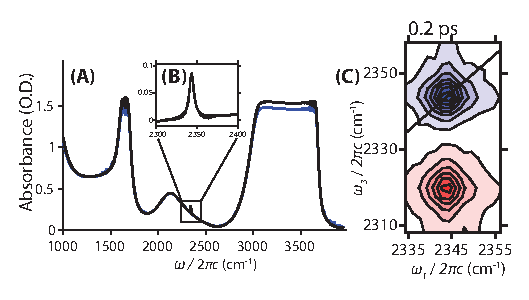
\includegraphics[scale=1.25]{./paper_01/fig1.eps}
  \caption[Linear and 2D-IR of \texorpdfstring{\ce{CO2} in \ce{H2O}}{carbon dioxide in water}]{\label{fig:CO2 in water}(A) FTIR spectrum of \ce{H2O} with (blue line) and without (black line) \ce{CO2} dissolved in it. \ce{CO2} \(\nu_3\) lies in the overtones and combinations bands from \ce{H2O} librational modes. (B) Inset of \(\nu_3\) with water background subtracted shows the Lorentzian character of the peak. (C) Purely absorptive 2D-IR spectrum of \(\nu_3\) in \ce{H2O} with \(t_2 = \SI{0.2}{\ps}\) shows that, in water, the line is nearly completely in the limit of homogeneous dynamics.}
\end{figure}

The other vibrational modes of \ce{CO2}, the symmetric stretch, \(\nu_1\), and the doubly degenerate bend, \(\nu_2\) and \(\bar{\nu}_2\), present distinct challenges for vibrational spectroscopy. The \(\nu_2\) modes are sensitive to the chemical environment of the \ce{CO2},\cite{Meredith1996,Kazarian2000} but are located in the crowded fingerprint region. The Raman active \(\nu_1\) is readily measured, but the lineshape is dominated by the Fermi resonance with the overtone of the \(\nu_2\);\cite{Cabaco2011} furthermore, it is a dark mode for IR.

Here, we demonstrate that the \ce{CO2} \(\nu_3\) mode reports on its local solvent environment by showing the sensitivity of the \(\nu_3\) frequency and dynamics to variation in solvent anion in a series of imidazolium ionic liquids; furthermore, we show that \(\nu_3\) reports a broad range of solvation timescales in these ionic liquids. We employ electronic structure calculations to investigate the mapping of vibrational frequencies onto structures of \ce{CO2}-anion-cation clusters. We show that, despite apparent complexity, the \ce{CO2} linear and 2D-IR lineshapes can be interpreted using simple and accurate physical models. Finally, we establish correlations between the measured dynamics of \ce{CO2} and the macroscopic properties of its ionic liquid solvent.

The paper is organized as follows. Initially, we present the analysis and interpretation of the linear \ce{CO2} spectrum (Section~\ref{sec:anions_linear}), including a discussion of its temperature dependence. Next, we describe the our results from electronic structure calculations on \ce{CO2}-anion-cation clusters and its relationship to our experimental data (Section~\ref{sec:vib_calcs}), followed by a simple model of \ce{CO2} that is able to reproduce the observed trends (Section~\ref{sec:freq-geom_disc}). We then present an overview of the 2D-IR spectra (Section~\ref{sec:anions_2DIR}), including a kinetic analysis of the observed shoulders and cross-peaks (Section~{\ref{sec:shoulders}), assignments of the spectral features (Section~\ref{sec:nu3_assignment}), and modelling of the main \(\nu_3\) peak (Section~\ref{sec:anions_2DIR_analysis}) and shoulders and cross-peaks (Section~\ref{sec:shoulders_modeling}). Finally, we present a discussion of the physical interpretation of our results (Section~\ref{sec:anions_interpretation}), conclusions (Section~\ref{sec:anions_conclusions}) and methods (Section~\ref{sec:anions_methods}).

\section{\texorpdfstring{\caps{Methods}}{Methods}}
\label{sec:anions_methods}

\subsection{Materials}
\label{sec:anions_methods_materials}

Ionic liquids were obtained from Ionic Liquids Technologies, Inc (IoLiTec), and used without further purification (except for \ce{[Im_{4,1}][BF4]}, which was purified prior to experiments using the procedure described by Giernoth and Bankmann.\cite{Giernoth2008}) Ionic liquid samples were stored in ambient conditions; however, prior to experiments, samples dried under vacuum at \SI{50}{\milli\torr}.

\subsection{FTIR}
\label{sec:anions_methods_ftir}

FTIR spectra were measured using a \ce{N2_{(g)}}-purged Nicolet 6700 FTIR instrument (ThermoFisher Scientific). Ionic liquid samples were loaded with \ce{CO2} (99.8\% purity, Matheson TRIGAS) in an airtight custom glass vial, with a septum that allows access to the \ce{CO2}-loaded ionic liquid. An aliquot of the liquid sample was sandwiched between two 2~mm-thick \ce{CaF2} optical windows (Crystran Ltd, UK) separated by a \SI{25}{\micron} Teflon spacer, which were held in a brass sample cell. The cell was assembled in a glove bag to limit adsorption of atmospheric water. Spectra were obtained for both the neat ionic liquid and for the ionic liquid loaded with \ce{CO2}.

For temperature-dependent measurements, the sample was temperature-controlled by using a cooling/heating recirculating chiller (Fisher Isotemp) to control the temperature of the sample cell holder. The sample temperature was monitored by measuring the temperature at the optical window using a thermocouple (National Instruments USB-TC01 J-type).

\subsection{2D-IR}
\label{sec:anions_methods_tdir}

\subsubsection{Generation of femtosecond mid-IR pulses}
\label{sec:anions_methods_tdir_generation}

The experiments utilize a commercial Ti:Sapphire chirped pulse amplifier laser system (\(\lambda = \SI{805}{\nm}\), \SI{5}{\kilo\hertz} repetition rate, \SI{120}{\fs} pulse duration) (Coherent Vitesse / Coherent Legend Elite).

A home-built optical parametric amplifier (OPA) generates the mid-IR pulses (\(\lambda = \SIrange{12}{2}{\micron}\)), corresponding to around \SIrange{830}{5000}{\wavenumber}. The OPA design leads to noise suppression in the resulting mid-IR pulses.\cite{Hamm2000} The spectral bandwidth after the OPA is about \SI{200}{\wavenumber}. For these experiments, we tune the OPA wavelength to \SI{4.3}{\micron}. Mid-IR pulse energy entering the 2D spectrometer is approximately \SI{2.2}{\micro\joule} per pulse.

\subsubsection{2D Spectrometer}
\label{sec:anions_methods_tdir_spectrometer}

The 2D-IR spectrometer uses a pump-probe geometry,\cite{Helbing2010} in which the first two mid-IR pulses travel collinearly to the sample. A Mach-Zehnder interferometer controls the coherence time \(t_1\) between these pulses. A delay stage after the interferometer controls the population time \(t_2\) between the second and third pulses. The signal, which contains both rephasing and non-rephasing components, is emitted in the direction of the probe pulse (\(\vec{k}_3\)), which also serves as a local oscillator to heterodyne the signal.

A 150 line/mm grating in a single monochromator disperses the signal in \(\omega_3\) onto a liquid \ce{N2}-cooled \(2 \times 32\) channel mercury cadmium telluride (MCT) detector. The signal in \(\omega_1\) is indirectly acquired by scanning along \(t_1\) using the Mach-Zehnder interferometer, and then applying a numerical Fourier transform to the resulting \(t_1\)-dependent signal at each data point in \(\omega_3\) (which also removes the transient absorption signal). The delay changes as the interferometer scans along \(t_1\) are acquired by comparing the interference pattern generated by a He:Ne beam which travels a parallel path through the interferometer.

A series of spectra in \(t_2\) are then acquired by varying the population time between the second and third laser pulses, and then obtaining a spectrum in \(\omega_1\) and \(\omega_3\) at each population time.

\subsection{Global Fitting and Bootstrapping}
\label{sec:anions_methods_fitting}

Global fitting of spectra utilizes a third-order response function formalism in the semi-impulsive limit, including the Condon approximation and also the approximation of the cumulant expansion truncated after second order. A constrained nonlinear optimization algorithm (\verb!fmincon! MATLAB) is used to minimize the magnitude of the sum of squared error between each data point in the set of spectra and a corresponding data point in a calculated spectrum. A bootstrapping algorithm \cite{numericalrecipes-92} establishes the error of the global fitting result. The global fitting algorithm was run using synthetic data sets composed of a random selection of the original data points taken with replacement. The distribution of the fitting parameters after 100 iterations provided the error estimate.

\subsection{Computational Details}
\label{sec:anions_methods_computational}

All calculations were performed with a development version of the Q-Chem program package\cite{Shao2015}, employing the B3LYP density functional, the 6-31G(d,p) basis set, and a (100,302) grid for the numerical quadrature. All SCF calculations were tightly converged to below \num{e-9}~a.u.\ for the DIIS error. Gas-phase geometry optimizations of free \ce{CO2} and the \ce{CO2}--ionic liquid clusters were converged to changes of \num{1d-8}~a.u.\ in the energy, \num{1d-6}~a.u.\ in the nuclear displacement, and \num{1d-6}~a.u.\ in the gradient. Optimized structures were confirmed as minima via harmonic frequency calculations using analytic Hessians. Frequencies were scaled by a factor of \num{0.9627} (Table 6 Merrick et al.)\cite{Merrick2007}.

For the calculations including the electrostatic and polarization effects of the ionic liquid with charge transfer disabled (``\(+ \Delta \omega_\mathrm{FRZ} + \Delta \omega_\mathrm{POL}\)'' in Figure~\ref{fig:decomposition}), absolutely localized molecular orbitals (ALMOs)\cite{Khaliullin2006} were employed, with the ionic liquid constituents as one combined fragment and the \ce{CO2} as another fragment. Solution of the ALMO equations is requested by setting \verb!frgm_method = gia!. Charge transfer between fragments is disabled by setting \verb!frgm_lpcorr = 0!. For the calculation of complementary occupied-virtual pairs (COVPs), an energy decomposition analysis (ALMO-EDA) calculation is performed where charge transfer is allowed (\verb!frgm_lpcorr = rs_exact_scf!).

\section{\texorpdfstring{\caps{Results and Discussion}}{Results and Discussion}}

\subsection{Linear IR Spectroscopy Results}
\label{sec:anions_linear}

The linear spectra of \ce{CO2} establish that the \(\nu_3\) mode is sensitive to the anion, and set the stage for discussing the spectroscopic features present in the 2D-IR spectra.

The \(\nu_3\) vibration absorbs strongly around \SI{2340}{\wavenumber} in a spectral region with no strong solvent absorbances (Figure~\ref{fig:FTIR}A). The lineshape of the \(\nu_3\) band (Figure~\ref{fig:FTIR}B) appears mostly Lorentzian, with a low frequency shoulder.
\begin{figure}
  \centering
  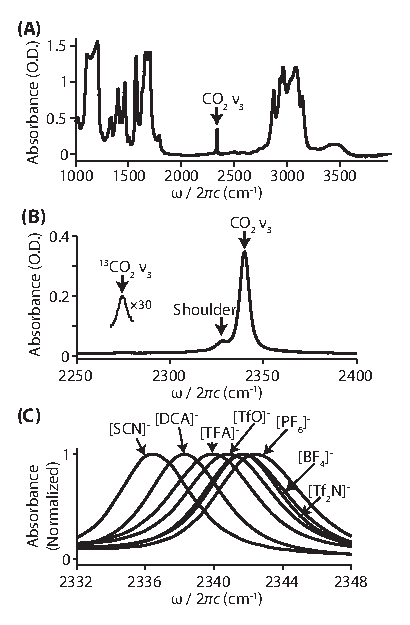
\includegraphics[scale=1.40]{./paper_01/fig2.eps}
  \caption[FTIR of \texorpdfstring{\ce{CO2}}{carbon dioxide} in ionic liquids]{\label{fig:FTIR} a) Absorption spectrum of \ce{CO2} in \ce{[Im_{4,1}]}[TFA] shows the intense antisymmetric stretch absorption at \SI{2340}{\wavenumber}; b) the background subtracted spectrum is Lorentzian with a shoulder at \SI{2328}{\wavenumber}, the \(\nu_3\) band of the \ce{^{13}C} isotopomer is located at \SI{2280}{\wavenumber}; c) The average vibrational frequency of the \(\nu_3\) absorption of \ce{CO2} shifts for different anions and the same \ce{[Im_{4,1}^+]} cation (background subtracted).}
\end{figure}

Changing the anion causes both the full-width at half-maximum (FWHM) and center frequency of \(\nu_3\) to change (Figure~\ref{fig:FTIR}C). We varied the anion, rather than the cation, because the anion dominates \ce{CO2} solubility in ionic liquids.\cite{anthonyJPCB-05,Cadena2004,Bhargava2007} Anions studied were hexafluorophosphate (\ce{PF6-}), tetrafluoroborate (\ce{BF4-}), bis-(trifluoromethyl\-sulfonyl)imide (\ce{Tf2N-}), triflate (\ce{TfO-}), trifluoroacetate (\ce{TFA-}), dicyanamide (\ce{DCA-}), and thiocyanate (\ce{SCN-}). The cation in all experiments was 1-butyl-3-methylimidazolium (\ce{[Im_{4,1}]}).

The \(\nu_3\) center frequency progressively redshifts from a maximum of \SI{2342.5}{\wavenumber} (\ce{[PF6-]}) to a minimum of \SI{2336}{\wavenumber} (\ce{[SCN]-}). The shoulder moves with the main absorption band and stays \(\sim\SI{12}{\wavenumber}\) lower in frequency.  Qualitatively, smaller, harder anions like \ce{[SCN]-} and \ce{[DCA]-} create a larger redshift than bulkier, softer anions like \ce{[Tf2N]-} and \ce{[TfO]-}, which is most likely a function of increased anionic charge density. The increased charge density could red-shift the \ce{CO2} center frequency though an increased local electric field (Stark effect), through charge transfer, or through inductive effects. Quantum chemistry calculations (Section~\ref{sec:vib_calcs}) help to disentangle the driving forces behind this qualitative trend.

The shoulder on the low frequency side of the main \(\nu_3\) transition could arise from several possible mechanisms, a ``hot-band'', a multiple-quantum transition, or different chemical environments. The temperature dependence of this feature is important in discriminating among these possibilities.

Temperature-dependent FTIR demonstrates that the shoulder on the low frequency side of the main \(\nu_3\) transition  is a hot band of the \(\nu_3\) mode (Figure~\ref{fig:hot band}A). Increasing temperature causes a decrease in intensity of the main peak and an increase in intensity of the shoulder, while conserving oscillator strength. The relative magnitude of the shoulder (\(\sim 10\%\) of the main band at room temperature) is similar to the expected relative excited state bending mode (\(\nu_2\)) population predicted by a Boltzmann distribution.

\begin{figure}
  \centering
  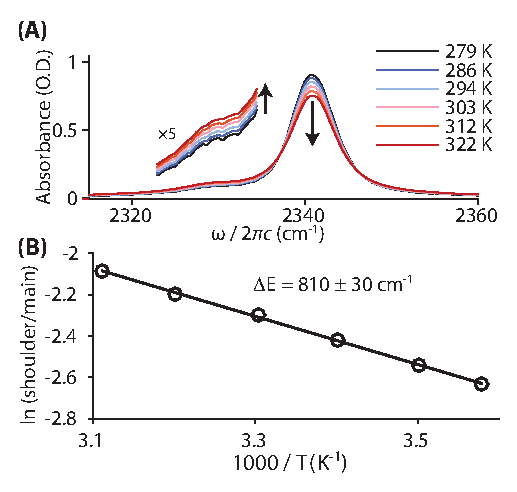
\includegraphics[scale=1.40]{./paper_01/fig3.eps}
  \caption[T-dependent FTIR of \texorpdfstring{\ce{CO2}}{carbon dioxide} in 1-butyl-3-methylimidazolium triflate]{\label{fig:hot band}(A) Temperature dependence of the \(\nu_3\) spectrum in \ce{[Im_{4,1}]}[TfO] shows transition of intensity from the main peak to the shoulder with increasing temperature, indicating a temperature-dependent two-state transition. (B) Relative intensity of shoulder to the main band (based on fitting to Voigt profiles) follows a van't Hoff temperature dependence, indicating an energy barrier of around \SI{800}{\wavenumber}, which closely follows the prediction from the temperature dependence of bending mode population.}
\end{figure}

We fit the spectra in Figure~\ref{fig:hot band}A to two Voigt profiles (one for the main peak, and one for the first shoulder seen on the 2D-IR).

A van't Hoff analysis of the logarithm of the relative peak heights against \(1/T\) gives an activation energy of \SI{810(30)}{\wavenumber}. This value is near the energy of the \(\nu_2\) bending vibration (\SI{667}{\wavenumber}). Residual gas lines and nonlinearity of the detector contribute to the systematic error of this measurement. Nevertheless, the temperature dependence strongly suggests that the first shoulder is due to one quantum of the bending mode which is excited thermally and is anharmonically coupled to the \(\nu_3\) mode.

The temperature dependence and hot-band assignment are important components of our interpretation of the shape of the 2D-IR spectra (Section~\ref{sec:shoulders}) and their time-dependence (Section~\ref{sec:shoulders_modeling}).

\subsection{Vibrational Frequency Calculations}
\label{sec:vib_calcs}

Electronic structure calculations provide a rationale for the observed trend in vibrational frequencies.

Harmonic frequency calculations reproduce the general trend that \(\nu_3\) progressively redshifts with decreasing anion size (Table \ref{tab:1}).  We simplify the solvated \ce{CO2} structure to a gas-phase cluster consisting of one \ce{CO2} with one cation-anion pair, with 1,3-dimethylimidazolium (\ce{Im_{1,1}}) as the cation. When scaled with the appropriate factor\cite{Merrick2007}, the simulations calculate vibrational frequencies within a few wavenumbers of the experimental value. The ordering of anions mostly agrees with experiment as well, the only outliers being \ce{[TFA]-} and \ce{[SCN]-}, which are located only \SI{2.3}{\wavenumber} apart.

The level of agreement between experiment and theory is good, given that the condensed phase environment is neglected. That such a simple representation reproduces the general trends so well suggests that the interactions of \ce{CO2} are dominated by local effects in its immediate surroundings. Future work will address the condensed phase effects by sampling representative structures from molecular dynamics simulations and repeating the analysis in the context of larger solvation shells.

Encouraged by the fact that the electronic structure calculations reproduce the experimental trends in \(\nu_3\) frequencies, we decompose the calculated vibrational frequencies into different components using absolutely localized molecular orbitals (ALMO), in analogy to ALMO energy decomposition analysis (ALMO-EDA).\cite{Khaliullin2006,Khaliullin2007,Khaliullin2008}

Unlike standard quantum chemical calculations, where individual molecular orbitals may delocalize over more than a single fragment, each ALMO is composed of atomic orbitals from a single fragment. This constraint allows us to control charge transfer between fragments and to quantify the interaction between fragments in physically intuitive terms.

The total vibrational frequencies \(\omega_{\mathrm{tot}}\) and vibrational shifts \(\Delta \omega_\mathrm{int}\) from gas phase (``free'') \ce{CO2} for each mode \(\nu\) may be written as:
\begin{equation}
  \omega_\mathrm{tot} = \omega_\mathrm{free} + \Delta \omega_\mathrm{int}
\end{equation}
where
\begin{equation}
  \Delta \omega_\mathrm{int} = \Delta \omega_\mathrm{GEOM} + \Delta \omega_\mathrm{FRZ} + \Delta \omega_\mathrm{POL} + \Delta \omega_\mathrm{CT}
\end{equation}
where \(\Delta \omega_\mathrm{GEOM}\) (geometric distortion) corresponds to the change in frequency caused by distortion of fragments from their free geometries to their cluster geometries, \(\Delta \omega_\mathrm{FRZ}\) (the frozen orbital interaction) results from the combined electrostatic interaction and Pauli repulsion between the filled, unrelaxed orbitals of each fragment, \(\Delta \omega_\mathrm{POL}\) (polarization) is due to the relaxation of a fragment's orbitals in the field of the other fragments, and \(\Delta \omega_\mathrm{CT}\) (charge transfer) is from occupied-virtual orbital donation between orbitals of different fragments.\cite{Ramos-Cordoba2011}

The cluster environment can affect the vibrational frequency of \ce{CO2} in two different ways. The first depends on the anharmonic potential surface of a free \ce{CO2} molecule. In a harmonic system, the spring constant, \(k\), uniquely determines the vibrational frequency for all nuclear positions (i.e., the curvature of a quadratic potential is constant). \ce{CO2}'s potential energy surface, however, is inherently anharmonic. Any change in geometry will thus cause a change in the \(\nu_3\) vibrational frequency. In other words, the cluster can change the \(\nu_3\) frequency just by shifting the location of minimum of the \ce{CO2} potential (\(\Delta \omega_\mathrm{GEOM}\)). The second results from changes in the local curvature of \ce{CO2}'s potential energy surface due to interactions with the surrounding cluster (\(\Delta \omega_\mathrm{FRZ} + \Delta\omega_\mathrm{POL} + \Delta \omega_\mathrm{CT}\)).

We focus on the following grouping of terms: (1) distortion of isolated \ce{CO2} to its cluster geometry (\(\Delta \omega_\mathrm{GEOM}\)), (2) the combined frozen orbital and polarization contributions through use of ALMOs (\(\Delta \omega_\mathrm{FRZ} + \Delta \omega_\mathrm{POL}\)), and (3) charge transfer between the fragments in the cluster (\(\Delta \omega_\mathrm{CT}\)).

The final frequency, \(\omega_\mathrm{tot}\), correlates most strongly with \(\Delta \omega_\mathrm{GEOM}\) (\(R^2 = 0.96\)), indicating that geometrical distortion of \ce{CO2} dominates the frequency shift. Depending on the particular geometry that \ce{CO2} adopts in the cluster, \(\Delta \omega_\mathrm{GEOM}\) can vary by \SI{\pm 6}{\wavenumber} (Figure~\ref{fig:decomposition}).\footnote{Since \(\omega\) normally refers to an angular frequency, this quantity might more rigorously be be called \(\Delta \omega_\mathrm{GEOM} / 2 \pi c\); however, for convenience of notation, we chose to use spectroscopic units uniformly in this section. That is, all frequencies are given in wavenumbers, rather than \si{\radian\per\second}.} Electrostatics and charge transfer both change the local curvature of the potential energy surface; however, their effects are mostly uniform across the ionic liquids studied. When we turn off charge transfer between fragments, \(\nu_3\) blue-shifts on average by \(\braket{\Delta \omega_\mathrm{FRZ} + \Delta \omega_\mathrm{POL}} =\) +\SI{2.8(6)}{\wavenumber}. Modelling the cluster geometry as a field of point charges increases this blue shift to +\SI{4.4(6)}{\wavenumber} (Supplementary Information), which may indicate that a point-charge representation of the cluster over-polarizes the QM region~\cite{Bakowies1996,Hu2011} Allowing charge transfer red-shifts the frequencies by $\braket{\Delta \omega_\mathrm{CT}} =$~-\SI{3.5(8)}{\wavenumber}.  Thus, both electrostatics and charge transfer change the local curvature of the \(\nu_3\) potential energy surface. The effects, however, are uniform and nearly cancel. The net result is that the inherent anharmonicity of the \ce{CO2} potential energy surface ultimately dominates the \(\nu_3\) frequency.

The geometrical distortion of the \ce{CO2} is driven by charge transfer. Using ALMOs and forbidding charge transfer during relaxation of the cluster removes the variance in \(\Delta \omega_\mathrm{GEOM}\) (Figure~\ref{fig:decomposition}B). Once again, both electrostatic and charge transfer interactions act uniformly on the frequency, leading to a negligible variance in \(\omega_\mathrm{tot}\). Without the geometrical distortion due to charge transfer, the vibrational frequencies for all clusters remain within $\pm2$~\si{\wavenumber} and no longer follow the experimental trend.

The essential point is that charge transfer and electrostatics only affect the vibrational frequency indirectly, through their coupling into the equilibrium \ce{CO2} nuclear geometry. The direct effects of electrostatics and charge transfer on the potential energy surface (and thus the effective spring constant) of \(\nu_3\) are uniform across ionic liquids studied and counteract each other.

This DFT-based analysis may over-emphasize charge transfer to some extent. It is well known that DFT over-delocalizes electrons due to self-interaction error, which might exaggerate the amount of charge transfer. In the context of gas-phase anion clusters, both DFT\cite{breen-JPCA12} and post-Hartree-Fock methods\cite{Muraoka2009} have also identified charge transfer as a driver of geometrical distortion of \ce{CO2}, so we expect that our qualitative picture will be robust with respect to the theoretical method. Future work will explore the quantitative differences between the different methods. Furthermore, although our cluster results agree well with experiment, we expect that the extended solvation environment neglected here may introduce screening effects not captured at the cluster level.\cite{Lee2011a}  A more sophisticated study of solvation effects could determine whether our finding, that charge transfer dominates the geometric effects which differentiate \ce{CO2} vibrational frequency shifts, is transferable to bulk ionic liquids.

These calculations demonstrate that the \(\nu_3\) frequency shift reflects a complex interplay between geometry, electrostatics, and charge transfer. The geometrical distortion is the most important factor in determining the final variation in vibrational frequency with anion identity; however, the equilibrium geometry of the \ce{CO2} itself ultimately depends on inductive effects, such as charge transfer.

\begin{table}
  \centering
  \caption[Experimental and calculated \texorpdfstring{\ce{CO2} \(\nu_3\)}{carbon dioxide antisymmetric stretch} vibrational frequencies]{\label{tab:1}Experimental and calculated \(\nu_3\) vibrational frequencies for \ce{CO2} in various imidazolium (experimental \ce{[Im_{4,1}]}, calculations [\ce{Im_{1,1}}]) ionic liquids. Calculations are carried out using a gas phase anion-cation-\ce{CO2} cluster at 0 K. The level of agreement between calculations and experimental results indicates that interactions of \ce{CO2} are dominated by local effects in its immediate surroundings.}
  \begin{tabular}{cccc}
    \toprule
    Anion & Expt. Freq. & Calc.\ Freq. & Calc.\ Freq. (scaled) \\
          & (\si{\wavenumber}) & (\si{\wavenumber}) & (\si{\wavenumber}) \\
    \midrule
    \ce{[PF6]-} & 2342.5 & 2437.7 & 2346.8 \\
    \ce{[Tf2N]-} & 2341.7 & 2435.8 &2344.9 \\
    \ce{[BF4]-} & 2341.7 & 2434.7 & 2343.9 \\
    \ce{[TfO]-} & 2340.9 & 2431.9 & 2341.2 \\
    \ce{[TFA]-} & 2339.9 & 2429.3 & 2338.7 \\
    \ce{[DCA]-} & 2338.4 & 2430.5 & 2339.8 \\
    \ce{[SCN]-} & 2336.5 & 2430.0 & 2339.4 \\
    \bottomrule
  \end{tabular}
\end{table}

\begin{figure}
  \centering
  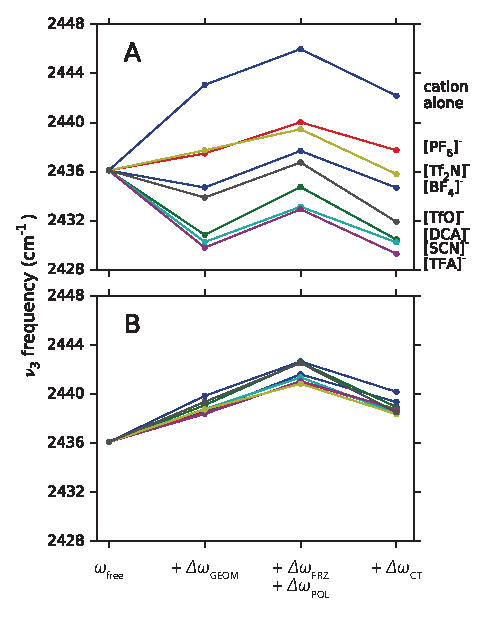
\includegraphics[scale=1.50]{./paper_01/fig4.eps}
  \caption[ALMO decomposition of \texorpdfstring{\ce{CO2} \(\nu_3\)}{carbon dioxide asymmetric stretch} frequency]{\label{fig:decomposition}Decomposition of the geometric, electrostatic, and charge transfer contributions to \ce{CO2} \(\nu_3\) vibrational frequency shifts. (A) The cluster geometry (including \ce{CO2}) was optimized while allowing charge transfer. (B) The cluster geometry was optimized using ALMOs to forbid charge transfer between fragments. The final frequency (\(\omega_\mathrm{tot} = \omega_\mathrm{free} + \Delta \omega_\mathrm{GEOM} + \Delta \omega_\mathrm{FRZ} + \Delta \omega_\mathrm{POL} + \Delta \omega_\mathrm{CT}\)) correlates most strongly with the change in frequency from geometric distortion (\(\Delta \omega_\mathrm{GEOM}\)).}
\end{figure}

\subsection{Frequency, Geometry, and  Charge Transfer Discussion}
\label{sec:freq-geom_disc}

To gain chemical insight into the charge transfer process, one can analyze the donor and acceptor orbitals of \ce{CO2} and the ionic liquid. This analysis sheds light on the nature of the geometrical distortion, which, in turn, leads to a simple model for the vibrational frequencies in terms of a few geometrical parameters.

We employ a complementary occupied-virtual orbital pair (COVP) analysis\cite{Khaliullin2008} to gain insight into the electronic structure effects underlying the charge transfer between \ce{CO2} and the solvent. COVPs provide a way to visualize charge transfer effects, where ``each COVP corresponds to an occupied orbital on one molecule donating charge to one specific (complementary) virtual orbital on the other molecule.''\cite{Khaliullin2009} These orbital pairs are constructed from a singular value decomposition of the occupied-virtual mixing matrix \(\mathbf{X}\) that describes charge transfer between the (polarized) fragments upon removing the ALMO fragment localization constraint. While \(\mathbf{X}\) contains, in general, excitations between all possible occupied-virtual pairs, the COVP representation of \(\mathbf{X}\) is diagonal and thus provides the most compact possible basis for describing charge transfer.  The associated singular values allow one to assess the contribution of a particular COVP to charge transfer, and typically one finds that only one or a few orbital pairs dominate the effect (as shown below in this study). The COVP analysis thus allows to conveniently identify and visualize the electron donor/acceptor orbitals pair(s) that significantly contribute to charge transfer.

Charge transfer to the \ce{CO2} originates from occupied orbitals on the anions. The charge is accepted by virtual orbitals on the \ce{CO2}. The virtual orbitals are a linear combination of the LUMO and LUMO+1 orbitals, which have \(\sigma^{*}\) and \(\pi^{*}\) character, respectively. Charge transfer from the anion has a strong linear correlation to the bend angle (\(R^2=0.84\)). Mechanistically, bending the \ce{CO2} allows \(\sigma^{*}\) and \(\pi^{*}\) to mix, lowers the energy of the acceptor orbital, and also maximizes the spatial overlap with the donor orbital. The amount of charge transferred (\SIrange{3}{5}{\milli\electron}) is small, but the resulting bend angle (\SIrange{3}{5}{\angstrom}) can be substantial (Table~\ref{tab:ct}).
\begin{table}
  \centering
  \caption[\texorpdfstring{\ce{CO2}}{Carbon dioxide} geometry dependence on charge transfer]{\label{tab:ct}Charge transfer from the anion to \ce{CO2} and from \ce{CO2} to the cation both contribute to the geometrical distortion of the \ce{CO2}. The most important geometrical degrees of freedom are the bend angle, \(\theta\) and the sum of the two carbonyl bond lengths, \(L\).}
  \begin{tabular}{ccccc}
    \toprule
    cluster & CT to \ce{CO2} (\si{\milli\electron}) & CT from \ce{CO2} (\si{\milli\electron}) & \(\theta\) (\si{\degree}) & \(L\) (\si{\angstrom}) \\
    \midrule
    \ce{[Im_{1,1}]+} & 0.079 & 2.251 & 0.07 & 2.3374 \\
    \ce{[PF6]-} & 3.336 & 1.012 & 3.79 & 2.3379 \\
    \ce{[Tf2N]-} & 2.493 & 1.603 & 2.64 & 2.3380 \\
    \ce{[BF4]-} & 4.558 & 1.264 & 4.51 & 2.3385 \\
    \ce{[TfO]-} & 3.009 & 2.339 & 4.01 & 2.3389 \\
    \ce{[TFA]-} & 5.131 & 1.618 & 5.22 & 2.3394 \\
    \ce{[DCA]-} & 3.376 & 2.259 & 4.99 & 2.3394 \\
    \ce{[SCN]-} & 3.317 & 1.323 & 4.35 & 2.3395 \\
    \bottomrule
  \end{tabular}
\end{table}

\ce{CO2} also donates charge back to the ionic liquid cluster, primarily to the cation. The amount of charge donated by the \ce{CO2} to the cation (\SIrange{-1}{-2}{\milli\elementarycharge}) is typically less than the charge donated from the anion, but nevertheless has specific consequences for the resulting geometry. The donor orbital from the \ce{CO2} is a mixture of \(\sigma\)-bonding and \(\pi\)-nonbonding character. The charge donation from the \ce{CO2} is linearly correlated to the carbonyl bond length differences (\(R^2 = 0.85\)). For the \ce{[Im_{1,1}][TfO]} cluster, which has the highest charge transfer from \ce{CO2} to the cation (\SI{2.32}{\milli\electron}), the \(\sigma\) character of the donating orbital causes the carbonyl nearest the cation to lengthen from the gas-phase \SI{1.169}{\angstrom} to \SI{1.175}{\angstrom} while the distal carbonyl contracts to \SI{1.163}{\angstrom}.

The effects of charge transfer to and from the \ce{CO2} can be incorporated into a simple model of the vibrational frequencies. The model is constructed in a vibrational local-mode basis. The effective one exciton vibrational Hamiltonian is

\begin{equation}
  H^{(1)} =
  \begin{pmatrix}
    \hbar\omega_1 & \beta\\
    \beta & \hbar\omega_2
  \end{pmatrix}
\end{equation}
where \(\omega_i\) is the local mode frequency of carbonyl \(i\) and \(\beta\) is the coupling between the two local modes. The diagonalized hamiltonian gives symmetric and antisymmetric linear combinations of the local modes as the vibrational eigenstates with energies \(\hbar\omega_s\) and \(\hbar\omega_a\). The splitting between symmetric and antisymmetric vibrations is twice the coupling constant, \(\hbar(\omega_s - \omega_a) = 2\beta\), and the average frequencies in local and normal modes are also equal \(\hbar(\omega_a + \omega_s)/2 = \hbar(\omega_1 + \omega_2)/2 = \alpha\).

The bend in the \ce{CO2} determines the change in the coupling constant between the local modes, \(\beta\) (\(R^2 = 0.94\)). The motion of the central carbon atom is the primary motion that couples the two carbonyls. When they are collinear, the motion of one carbonyl directly influences the other. Bending the \ce{CO2} means the carbonyls are no longer collinear, which means that the projection of one local vibration on the other decreases. This decrease, in turn, decreases the effective coupling constant.

The sum of the \ce{CO2} bond lengths \(L\), is correlated to the \(\alpha\) (\(R^2 = 0.998\)). The dependence of \(\alpha\) on the geometry of the molecule is not as straightforward than that of \(\beta\). In the strong coupling limit, \(\beta \gg |\hbar\omega_2-\hbar\omega_1|\), the symmetric and antisymmetric stretching frequencies only depend on the average frequencies, \((\hbar\omega_1 + \hbar\omega_2)/2\). As such, the geometrical asymmetry induced by charge transfer from the \ce{CO2}, which weakens one bond and strengthens the other, is largely averaged out. Only a weak correlation between the charge donated from the \ce{CO2} and the \(\alpha\) remains. The sum of the bond lengths, \(L\), however, reports exactly this difference in total bonding strength. Though the changes in \(L\) are minute (\(\sim \SI{0.001}{\angstrom}\)), the effect on the vibrational frequencies is not.

Because of the strong linear correlation with these two geometrical variables, we propose that the simplest model of the scaled vibrational frequencies is \(\alpha(L)\) and \(\beta(\theta)\), where
\begin{equation}
  \alpha(L) = \SI{9523.8}{\wavenumber} - \left(3415.3~\mathrm{cm}^{-1} \mathrm{\AA}^{-1}\right) L %scaled 0.9627
\end{equation}
and
\begin{equation}
  \beta(\theta) = \SI{-515.7}{\wavenumber} + \left(1.12~\mathrm{cm}^{-1} \mathrm{deg}^{-1}\right)\, \theta, %scaled 0.9627
\end{equation}
where \(\alpha\) and \(\beta\) are in units of \si{\wavenumber}, \(L\) is in \si{\angstrom}, and \(\theta\) is in degrees. The one exciton Hamiltonian
\begin{equation}
  H^{(1)} =
  \begin{pmatrix}
    \alpha(L) & \beta(\theta)\\
    \beta(\theta) & \alpha(L)
  \end{pmatrix},
\end{equation}
% TODO SI
reproduces the scaled harmonic frequencies with an RMS error of \SI{1.2}{\wavenumber} and the experimental frequencies with an RMS error of \SI{4}{\wavenumber}.\footnote{See section~\ref{paper_01:sec:SI} for 2D-IR spectra of \ce{CO2} in each ionic liquid, as well as a comparison of center line slope and global fitting results for correlation times, and more detailed computational results. Additionally, there is information on fitting of the one exciton Hamiltonian model for unscaled frequencies, and vibrational frequency calculations of \ce{CO2} in a field of point-charges that approximates the cluster geometry.}

Following a detailed investigation of the charge transfer, the participating orbitals, and the effects of charge transfer on the \ce{CO2} geometry, we have put forward a simple model that successfully reproduces the calculated vibrational frequencies and, to a reasonable extent, the experimental frequencies, with no free parameters.

\subsection{2D-IR Spectroscopy Overview}
\label{sec:anions_2DIR}

While linear spectroscopy shows the sensitivity of \ce{CO2} to its local environment, it cannot address the ultrafast dynamics of the chromophore. 2D-IR, however, directly reports on the dynamic structural relaxation around \ce{CO2}. 2D-IR of \ce{CO2} in \ce{[Im_{4,1}]}[TFA] introduces many of the features that are general across all of the ionic liquids studied.

The 2D spectra of the \(\nu_3\) mode of \ce{CO2} in \ce{[Im_{4,1}]}[TFA] (Figure~\ref{fig:example 2D}A and B) show the main \(\nu_3\) band, two diagonal shoulders, and cross-peaks between them. The observed peaks cannot be explained without also keeping track of the states of the \ce{CO2} symmetric stretch and bending modes in the vibrational state. The total vibrational wavefunction is specified by $|\nu_1 \nu_2^l \nu_3 \rangle$, where \(\nu_1\) is the number of quanta in the symmetric stretch, \(\nu_2\) is the number of quanta in the bending mode, $l$ is the vibrational angular momentum quantum number of the bending mode, and \(\nu_3\) is the number of quanta in the antisymmetric stretch.

The main band consists of a pair of intense peaks corresponding to the $|00^00\rangle\rightarrow|00^01\rangle$  and $|00^01\rangle\rightarrow|00^02\rangle$ (1a and 1b) transitions, separated by the anharmonicity of \(\nu_3\) (\(\sim \SI{24}{\wavenumber}\)). Due to ground state bleach, 1a appears as a negative (blue) feature, while 1b, from excited state absorption, is a positive (red) feature. The \(\nu_3\) shoulder appears as a pair of small peaks (2a and b), shifted along the diagonal by \SI{-12}{\wavenumber} in \(\omega_1\) and \(\omega_3\). A second apparent shoulder, not seen on FTIR, presents as a pair of smaller peaks (1e and 1f), shifted along the diagonal from the main band by \SI{-24}{\wavenumber} in \(\omega_1\) and \(\omega_3\). At early population times, there is an apparent cross-peak between the main peak and second shoulder (1c). Cross-peaks grow in between the first shoulder and main peak (2-1a and b, 1-2b) over \(t_2\). The expected cross-peak 1-2a cannot be seen due to cancellation with the overwhelming opposite signal from the 1b.

The combination of \ce{CO2}'s high molar absorptivity (\(\sim \SI{1000}{\per\Molar\wavenumber}\)) and the \(\varepsilon^2\) dependence of the third-order signal causes the 2D signal from \ce{CO2} to dominate the spectrum in intensity. Contributions from solvent overtones in the background are smaller than the level of noise in the spectrum. Thus, the 2D signal reflects the vibrational modes of \ce{CO2}, rather than solvent background, and the solvent can only affect the 2D spectrum through intermolecular couplings with \ce{CO2} vibrational modes.

\begin{figure}
  \centering
  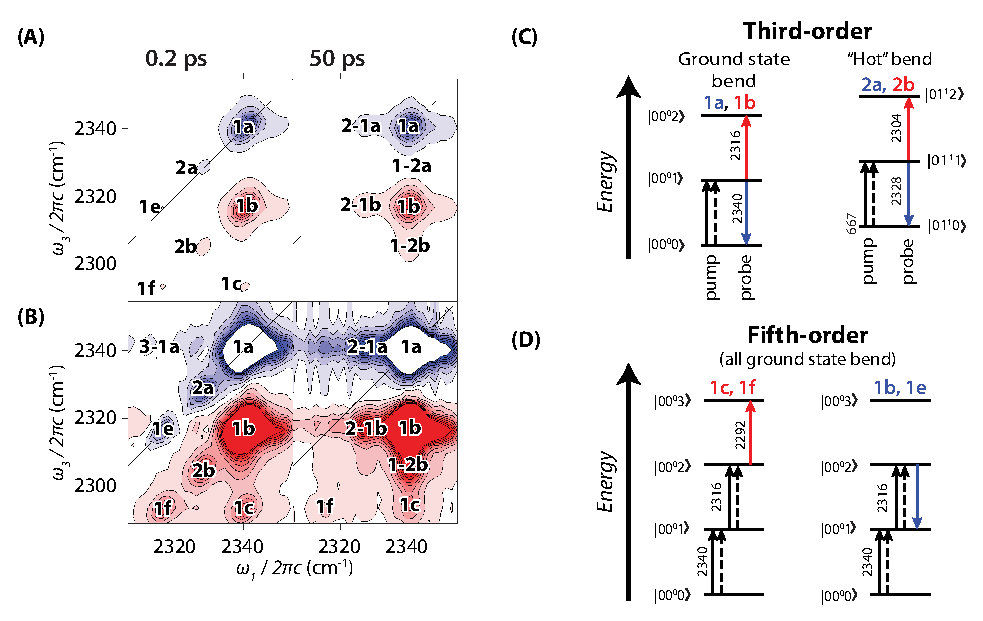
\includegraphics[scale=1]{./paper_01/fig5_update4.eps}
  \caption[2D-IR spectra of \texorpdfstring{\ce{CO2}}{carbon dioxide} in ionic liquids]{\label{fig:example 2D}\textbf{(A)} 2D-IR spectrum of \ce{CO2} in \ce{[Im_{4,1}][TFA]} at \(t_2\) = \SIlist[list-units = single]{0.2;50}{\ps}. The peak labels correspond to transitions in (C) and (D). \textbf{(B)} The same spectrum as (A) with contours limited to 10\% of the maximum in the $z$-direction. Structure of the diagonal shoulders and cross-peaks can be seen much more readily. \textbf{(C) and (D)} Vibrational energy level diagrams for observed third-order (C) and fifth-order (D) bands of \ce{CO2} in \ce{[Im_{4,1}][TFA]}. Quantum numbers correspond to $|\nu_1 \nu_2^l \nu_3\rangle$. Transition frequencies are labeled in wavenumbers (\si{\wavenumber}), and a label corresponding to the peaks in A and B. The color of the label indicates whether the expected peak is negative (blue) or positive (red).}
\end{figure}

The unambiguous spectral diffusion of 1a and 1b over the \SI{50}{\ps} population time demonstrates that the line is not entirely in the motional narrowing (homogeneous) limit. That is, \(\nu_3\) will allow us to resolve the dynamics of structural relaxation around \ce{CO2}.

The observations of a complex pattern of peaks and of spectral diffusion on a tens of picoseconds timescale for \ce{CO2} in \ce{[Im_{4,1}]}[TFA]  are general features of the spectra in all of the tested ionic liquids and are described in detail in the next two sections.

\subsection{2D-IR Shoulders and Cross-Peaks}
\label{sec:shoulders}

\begin{figure}
  \centering
  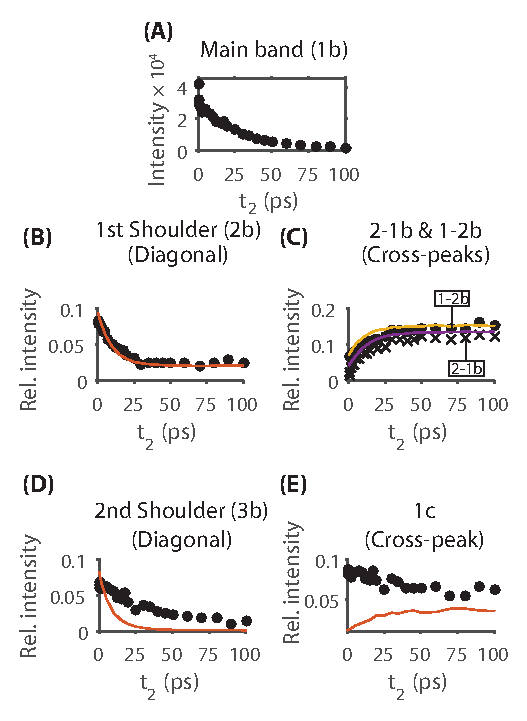
\includegraphics[scale=1]{./paper_01/fig6.eps}
  \caption[\texorpdfstring{\ce{CO2}}{Carbon dioxide} in IL bending mode kinetics]{\label{fig:shoulder kinetics}Kinetic analysis of \ce{[Im_{4,1}]}[TFA]. (A) Absolute intensity of the main peak (1b) with increasing \(t_2\). Decreased intensity results from both orientational and population relaxation. (B)-(E) show intensities relative to A. Discrete data points represent experimental data, while lines show data from stochastic simulations (Section~\ref{sec:shoulders_modeling}). (B) and (C), which result from the first diagonal shoulder (2b) and its cross-peaks with the main band (1-2b / 2-1b) show good agreement between experimental and simulated kinetics. (D) and (E), which result from the second diagonal shoulder (3b) and the apparent cross-peak (1c) show distinct kinetics, which cannot result from the same stochastic bending mode fluctuations, and point to a direct transition.}
\end{figure}

Careful analysis of the relative kinetics of the diagonal peaks and cross-peaks (Figure~\ref{fig:shoulder kinetics}) provides insight into how the coupling of \ce{CO2} vibrational modes and their stochastic dynamics create the observed spectrum.

Orientational and vibrational relaxation of \ce{CO2} cause a decrease in spectral intensity over \(t_2\). The main peak (1b) shows an initial rapid decrease in intensity from orientation relaxation, followed by a slower decay over \(\sim \SI{100}{\ps}\), from vibrational relaxation processes. Polarization-controlled studies can remove the contribution from orientational relaxation, and provide an explicit assessment of vibrational relaxation rate.\cite{hamm_concepts_2011,Hochstrasser2001}

The shoulders and cross-peaks are significantly weaker than the main peak, and also relax over \(t_2\); however, analysis of their kinetics relative to the main band reveals the underlying stochastic dynamics of \ce{CO2} vibrational modes.

The first diagonal shoulder (2b) decays more quickly than the main band, decreasing to a minimum intensity at \(\sim \SI{25}{\ps}\) followed by a (relative) steady state (Figure~\ref{fig:shoulder kinetics}). Cross-peaks between the first shoulder and the main band (2-1b and 1-2b) start at a minimum intensity, and then increase, before reaching a relative steady state by 25 ps. This behavior points to dynamic exchange between \(|00^01\rangle\) and \(|01^11\rangle\), which give rise to the diagonal peaks (Section~\ref{sec:shoulders_modeling}).

The second diagonal shoulder (3b) decreases in intensity relative to the main band, but more slowly than the first shoulder. The apparent cross-peak 1c decreases in relative intensity over \(t_2\) with slower kinetics than the second shoulder. This behavior contrasts with that of the cross-peaks 1-2b and 2-1b, and indicates that 1c arises from a direct vibrational transition, rather than dynamic exchange.

\subsection{Peak Assignment}
\label{sec:nu3_assignment}
The Dunham expansion for anharmonically coupled vibrational modes provides a theoretical framework for building an analysis of coupled vibrational modes:
\begin{equation}
  \label{eq:Dunham expansion}
  E = \sum_{i} \hbar \omega_i \left( n_i + \frac{1}{2} \right) + \sum_{ij} x_{ij} \left( n_i + \frac{1}{2} \right) \left( n_j + \frac{1}{2} \right)
\end{equation}
where $\omega_i$ is the frequency of the mode, $n_i$ is the number of quanta in the mode, and $x_{ij}$ are anharmonic coupling constants. It directly follows that the energy of a particular mode is given by:
\begin{equation}
  \label{eq:anh_coupled_energy}
  \nu_{n_k \rightarrow n_k + 1} = \nu_k + 2n_{k}x_{kk} + \sum_{i \neq k} x_{ij}n_{i},
\end{equation}
which implies that transition energy will decrease by \(x_{ij}\) for every quantum of energy in an anharmonically coupled mode.\cite{Botan2008} Gas phase vibrational calculations predict \(x_{23} \approx \SI{-12}{\wavenumber}\) per quantum in \(\nu_2\).\cite{Taylor1993,Dressier1997}

The first shoulder can then be explained by anharmonic coupling of excited state bending modes with the asymmetric stretching mode. This coupling causes a frequency shift of \SI{-12}{\wavenumber}, and creates a shoulder on the linear and the 2D spectra (peaks 2a/2b on 2D-IR). Stochastic fluctuations in thermally populated bending modes cause dynamic 2D-IR cross-peaks.

This mechanism for dynamic cross-peaks is not unique to \ce{CO2} in ionic liquids; however, it is a nearly ideal system in which to observe and analyze it. The narrow total linewidth (\(\sim \SI{6}{\wavenumber}\)), combined with a large anharmonic coupling constant (\(x_{23} = \SI{-12}{\wavenumber}\)), leads to clear segregation of the resulting frequencies into distinct peaks. The difference in energy between the ground and first excited state \(\nu_2\) modes is only around \(3k_{\textrm{B}}T\), which is low enough to be thermally accessible, but high enough to be quantized. Finally, the rate of stochastic fluctuations in bending mode states is slow enough to preserve distinct diagonal bands at short population times, but fast enough to allow dynamic cross-peaks over the timescale of the experiment (\(\sim \SI{100}{\ps}\)).

Alternative hypotheses can be ruled out. There are two possibilities that need to be addressed. First, the shoulder is often assigned to a multiquantum transition. Second, the shoulder and cross-peaks could be due to chemical exchange.

The first \(\nu_3\) shoulder in our spectra is also present in the FTIR of \ce{CO2} dissolved in organic liquids and many polymers, and is often attributed to a multiquantum transition $\nu_3 + \nu_2 - \nu_2$,\cite{Culp2010,Cunliffe-Jones1969,Kazarian1996,Meredith1996,Dobrowolski1992}  where the difference in energy is attributed to splitting of normally degenerate \ce{CO2} \(\nu_2\) and $\bar{\nu}_2$ bending modes. (This combination should perhaps be written as $\nu_3 + \nu_2 - \bar{\nu}_2$ or $\nu_3 + \bar{\nu}_2 - \nu_2$, but is typically presented without distinguishing between the two bending modes.) This hypothesis fails on several accounts. First, such a multiquantum transition is harmonically forbidden, so the transition dipole moment should be significantly lower than for the one quantum \(\nu_3\) transition. The intensity of the shoulder, however, directly follows a Boltzmann distribution for the \(\nu_2\) bending modes, which implies that the magnitude of the transition dipole moment is roughly equal for both the fundamental and this multiquantum transition.

Second, with this mechanism, a shoulder on the high frequency side of the fundamental should accompany the observed shoulder on the low frequency side. That is, there is no clear reason why the transition $\nu_3 + \nu_2 - \bar{\nu}_2$, would be strongly allowed, but $\nu_3 + \bar{\nu}_2 - \nu_2$ would not. Third, this hypothesis assumes that the splitting of the bending modes is an identical \SI{12}{\wavenumber}, but this is not the case.\cite{Kazarian2000}
Finally, in the 2D spectrum, this combination band would give rise to cross-peaks between the first shoulder and the main band (since each a \ce{CO2} molecule could undergo either transition with excitation), which would be present at the earliest population times, and would only relatively decay (rather than relatively increase) with \(t_2\). This behavior contradicts the observed spectral kinetics.

The temperature dependence of the shoulder (Figure~\ref{fig:hot band}) also excludes different chemical environments (such as multiple equilibrium geometries of a \ce{CO2}-anion interaction) undergoing chemical exchange. In this hypothesis, the most intense feature would be due to free \ce{CO2} and the shoulder to \ce{CO2} with a stronger chemical interaction. The growth of the cross-peaks would correspond to the exchange of these populations. However, the free \ce{CO2} band should be entropically favored and increase with increasing temperature while the shoulder should be enthalpically favored and decrease with increasing temperature. The opposite is observed, so this hypothesis can be ruled out. Additionally, the equal relative energy spacing of the diagonal shoulders from the main band for \ce{CO2} in every ionic liquid studied strongly suggests that the additional peaks arise from the \ce{CO2} itself, rather than from distinct chemical environments.

In contrast, the explanation of anharmonic coupling between \(\nu_2\) and \(\nu_3\) fits the temperature dependence, the transition dipole scaling, and accounts for the cross-peak kinetics. In our picture, each step requires only a one quantum transition for each peak, explains the presence of a shoulder on only one side of the fundamental, and correctly reproduces the cross-peak kinetics (over \(t_2\)) between the first shoulder and main band due to thermal excitation and de-excitation of the bend.

The apparent cross-peak 1c, as well as the second apparent shoulder (1e and 1f) are fifth-order signals, as can be shown by pump power-dependence, frequencies, and sign show that it is a fifth-order signal, as are several other features. Assignments of the \(\nu_3\) 2D-IR spectrum of carbon dioxide in 1-butyl-3-methylimidazolium trifluoroacetate \ce{[Im_{4,1}][TFA]}, are given in  Figure~\ref{fig:example 2D} and Table \ref{tab:fifth_order}).

The magnitude of third-order signal is linear in pump light intensity, since there are two pump electric field interactions, while that of fifth-order signal (with four electric field interactions) is quadratic. We assessed the magnitude of each peak when the pump power was changed by a factor of two (Table \ref{tab:fifth_order}). There is a clear distinction between the pump power dependence of the third order signals (1a, 1b, 2a, 2b, and their population exchange cross-peaks) and the fifth order signal (1c, 1e, 1f, and 31a). The reported intensity ratio is the ratio of volumes of a single peak when the pump power doubles. Thus, for the main `red' peak (1b: \(\nu_3\) excited state absorption with ground state \(\nu_2\)), peak volume goes up by a factor of \num{2.2 +- 0.1} when pump power doubles. Peak 1c's volume, however, increases by a factor of \num{3.3 +- 0.2}.
% TODO this bit here must come from the comment/erratum?
\begin{figure}
  \centering
  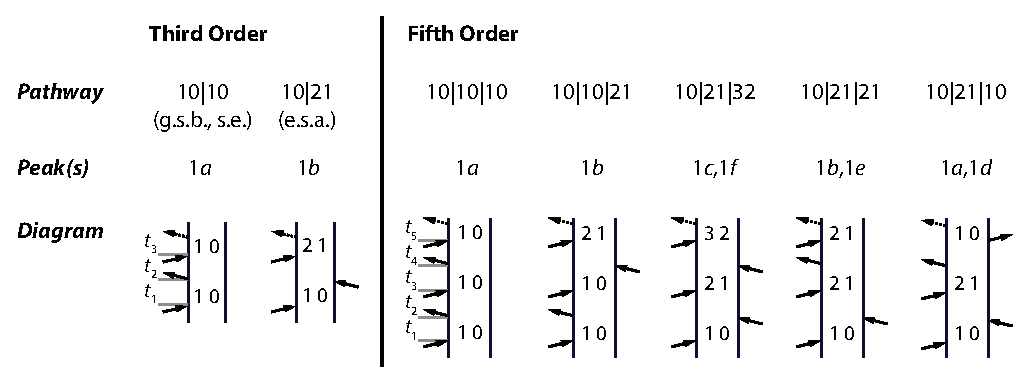
\includegraphics[scale=0.85]{./paper_01/sgr_pathways_02.eps}
  \caption[Double-sided Feynman diagrams for 3rd and 5th order signals]{\label{fig:Feynman}Double-sided Feynman diagrams, pathway labels, and peaks for third- and fifth-order peaks in the \ce{CO2} 2D-IR spectrum (non-rephasing pathways shown). Labels for pathways correspond to those used by Garrett-Roe and Hamm in their description of purely absorptive 3D-IR spectra.\cite{Garrett-Roe2009b} In a three optical pulse experiment (like 2D-IR), only two of the three coherences of a fifth-order signal can be resolved. Thus, depending on whether up-pumping occurs during the first or second pump pulse, either \(t_1\) or \(t_3\) will be unresolved in the fifth-order pathways. This effect can lead to multiple peaks on the 2D-IR spectrum from a single fifth-order pathway.}
\end{figure}

The fifth-order perturbative pathways have previously been described by Garrett-Roe and Hamm for 3D-IR (five IR pulse) spectroscopy.\cite{Garrett-Roe2009b} The assignment of a ``name'' for each fifth-order pathway (Table~\ref{tab:1} \& Figure~\ref{fig:Feynman}) follows the scheme used by Garrett-Roe and Hamm, where pathways are described by listing the vibrational quantum numbers of the three coherent states that contribute to them. Non-rephasing diagrams are shown for all pathways.

Since a 2D-IR experiment only has two coherence times (which give two frequency axes), we can only resolve two of the three coherences in the fifth-order pathway. When up-pumping occurs during the first two (``pump'') pulses, either \(t_1\) or \(t_3\) will be unresolved. Thus, each pathway can give two spectral peaks on a 2D-IR spectrum, if the coherent frequencies in \(t_1\) and \(t_3\) differ.  For fifth-order pathways in Table \ref{tab:1}, the coherence noted in parenthesis does not contribute to the observed peak, since oscillation of the first coherence will not be observed when there are multiple electric field interactions during a single 100 fs pulse. That is, the pathway \(10|21|32\) contributes to peaks 1c and 1f. Peak 1f results from up-pumping during the first pump pulse, $\left(10\right)|21|32$, and thus only the $|2\rangle\langle1|$ and $|3\rangle\langle2|$ coherences are observed. Peak 1c results from up-pumping during the second pulse, $10|\left(21\right)|32$, and thus only the $|1\rangle\langle0|$ and $|3\rangle\langle2|$ coherences are observed. The center frequency and sign of the peak amplitude for each observed fifth order peak matches that predicted by the corresponding fifth-order pathway (Table \ref{tab:1}).

The peaks 1c, 1e, 1f, and 3-1a are fifth-order signals, not cascading third-order signals. Two of the peaks, 1c and 1f, cannot be generated by a cascade, because they involve walking up the vibrational ladder to a $|3\rangle\langle2|$ coherence. Given the presence of these unambiguously direct fifth-order signals, we would expect to to find spectra contributions from other fifth-order pathways. Peaks 1e and 3-1a are located where we would predict additional fifth-order signal. The correspondence of the sign of the signal to those predicted by a direct fifth-order pathway is also important, because the relative signs of cascading third-order signals and fifth-order signals are opposite (due to the difference of $i^2$ in the pre-factor in the infrared). Furthermore, the relative magnitudes follow the predictions based on the various pathways through population states and harmonic transition dipole moment scaling.\cite{Garrett-Roe2009b} Finally, the relative peak intensities, including those of direct third-order signals, do not substantially vary with the concentration of the chromophore. Cascaded signals scale proportionally to $c^2$, and thus would not scale with the other peaks on the spectrum.

\setlength{\tabcolsep}{0.4em}
\begin{table}
  \centering
  \caption[Assignment of \texorpdfstring{\ce{CO2}}{carbon dioxide} features to 3rd or 5th order]{\label{tab:fifth_order}Peak parameters related to the assignment of peaks in the 2D-IR spectrum of \ce{CO2} in \ce{[Im_{4,1}][TFA]} to third-order or fifth-order signal. Pathways are labeled with the non-rephasing coherences they exhibit. Parenthetical coherences are not observed due to the timing of up-pumping (thus, 10|(21)|32 indicates a pathway with observed 2D-IR frequencies of $(\omega_1,\omega_3 = \omega_{01},\omega_{23})$.}
  \begin{tabular}{c c c c c c}%{ p{1.5cm} p{2.5 cm} p{1.75cm} p{1.5cm} p{2.5cm} } %
    \toprule % TODO clean up
    Peak Label & Center (\(\omega_{1}, \omega_{3}\)) & Peak Vol. Ratio\footnote{Factor by which the volume of the indicated peak increased when pump power was doubled.}  & Sign & Order & Pathway\footnote{g.s.b./s.e.: Ground state bleach / stimulated emission. e.s.a.: Excited state absorption. `Hot' peaks refer to peaks resulting from thermal excitation of the \(\nu_2\) bending mode. Numerals for Feynman pathways of fifth-order peaks from Garrett-Roe and Hamm.\cite{Garrett-Roe2009b} Subscripted `a' and `b' indicate whether up-pumping occurred on the first or second pulse.} \\
    \midrule
    1a & (2341.5, 2341.5) &$2.2 \pm 0.01$ & -- & 3 & $10|10$ (g.s.b./s.e.)  \\
    1b & (2341.5, 2317.5)&$2.2 \pm 0.02$ & + & 3 & $10|21$ (e.s.a.)   \\
    2a & (2329.5, 2329.5) &$1.9 \pm 0.03$ & -- & 3  & `hot' g.s.b./s.e. \\
    2b & (2329.5, 2305.5) &$2.5 \pm 0.1$ & + & 3  & `hot' e.s.a.  \\
    21a & (2329.5, 2341.5) & $1.7 \pm 0.2$ & --& 3  & pop. exch. \\
    21b & (2329.5, 2317.5) & $2.4 \pm 0.04$ & + & 3 & pop. exch. \\
    1e & (2317.5, 2317.5) & $3.8 \pm 0.2$ & -- & 5 & $\left(10\right)|21|21$ \\
    1f & (2317.5, 2293.5) & $3.5 \pm 0.1$ & + & 5  & $\left(10\right)|21|32$ \\
    1c & (2341.5, 2293.5) & $3.3 \pm 0.2$ & + &5 & $10|\left(21\right)|32$  \\
    31a & (2317.5, 2341.5) &$3.4 \pm 0.4$ & + & 5 & $\left(10\right)|21|10$ \\
    \bottomrule
  \end{tabular}
\end{table}

\subsection{Modelling of Main Band}
\label{sec:anions_2DIR_analysis}

The 2D peak of a specific vibrational mode encodes the frequency-fluctuation correlation function (Equation \ref{eq:FFCF}) in its lineshape. Lineshape analysis can extract the timescale of structure relaxation around that mode, by quantifying spectral diffusion, or change in diagonal character (or ellipticity), of a peak over \(t_2\).

The intense \(\nu_3\) peak clearly exhibits spectral diffusion in each ionic liquid studied (Figure~\ref{fig:all 2D}). Qualitatively, at early population times, the main \(\nu_3\) peaks have diagonal character. As a function of the population time, \(t_2\), the peaks become rounder. The rate of \(\nu_3\) spectral diffusion varies in the ionic liquids tested, indicating a broad range of timescales for structural relaxation in the different solvents. The rate is slowest in \ce{[Im_{4,1}]}[\ce{PF6}] (Figure~\ref{fig:all 2D}A) and fastest in \ce{[Im_{4,1}]}[DCA] (Figure~\ref{fig:all 2D}C). The vibrational relaxation time slow enough to allow us to measure over \SI{100}{\ps} of dynamics.

\begin{figure}
  \centering
  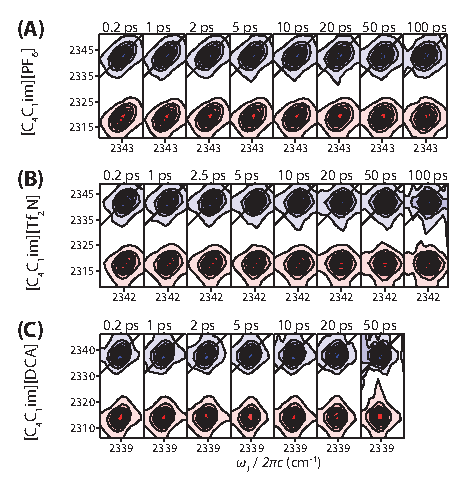
\includegraphics[scale=1.40]{./paper_01/fig7.eps}
  \caption[Experimental 2D-IR spectra of \texorpdfstring{\ce{CO2}}{carbon dioxide} in \ce{[Im_{4,1}][X]}]{Experimental 2D-IR spectra of \ce{CO2} in \ce{[Im_{4,1}]} (A) \ce{[PF6]}, (B) \ce{[Tf2N]}, and (C) [DCA] show the range of timescales for spectral diffusion in \(\nu_3\). Spectral diffusion results from local structural relaxation around \ce{CO2}. Spectral modelling quantifies the timescale of this structural relaxation, and indicates that the timescale varies by up to an order of magnitude between ionic liquid solvents, and that \ce{CO2} dynamics are likely gated by anion dynamics in these ionic liquids. Spectra for \ce{CO2} in other ionic liquids tested can be found in figure~\ref{paper_01:fig:SI_all_2D}.}
  \label{fig:all 2D}
\end{figure}

We used a global fitting algorithm to quantify the rate of spectral diffusion for \(\nu_3\) in each ionic liquid (Figure~\ref{fig:all 2D}). The main peak in the 2D spectrum is sufficiently separated from the shoulders that it can be treated independently. Simulated spectra were calculated using a third-order response function formalism in the semi-impulsive limit. The frequency-fluctuation correlation function
\begin{equation}
  \label{eq:c2}
  c_{2}(t) = \frac{\delta(t)}{T_2} + \Delta^2 \exp \left( -\frac{t}{\tau_c} \right),
\end{equation}
corresponds to a physical system in which \ce{CO2} senses two distinct timescales of motion. Fast motions, in the homogeneous limit, are modeled by first term, which describes a loss of correlation that is too fast to be quantified. In the time domain lineshape function, this leading term describes exponential decay in the ensemble response from dephasing, (with time constant \(T_2\)); the resulting lineshape in frequency space is a Lorentzian with FWHM of \(\left( \pi T_{2} \right)^{-1}\).

The second term corresponds to processes in the spectral diffusion regime, which create a Kubo lineshape. In the slow modulation limit (where \(\tau_c \Delta \gg 1\)), correlations do not change over the timescale of the molecular response. The resulting lineshape function describes a time-domain Gaussian with a variance of \(\Delta^{-2}\); the corresponding lineshape in frequency space is a Gaussian with FWHM of \(2.355\Delta\).

The analytical lineshape function:
\begin{equation}
  \label{eq:g(t)}
  g(t) = \frac{t}{T_2} + \Delta^2\tau_c^2 \left[ \exp{\left( -\frac{t}{\tau_c} \right)}
	+ \frac{t}{\tau_c} - 1 \right],
\end{equation}
can be used to calculate 2D spectra. Normalization of spectra before fitting removes any contribution from vibrational or orientational relaxation, which we do not model. A constrained nonlinear optimization algorithm globally fits the calculated spectra to experimental spectra by minimizing the sum of squares difference between the data and calculation. The algorithm optimizes \(T_2\), \(\tau_c\), and \(\Delta\), in addition to the central frequency, anharmonicity, the $|00^01{\rangle} \rightarrow |00^02{\rangle}$ transition dipole moment, and the phase. The resulting spectral diffusion time, \(\tau_c\), shows good agreement with that obtained by center line slope (CLS) analysis\ref{anionSI_CLS}.

Experimental and optimized calculated spectra agree in terms of overall lineshape and rate of spectral diffusion (Figure~\ref{fig:TFA 2D fit}). The resulting lineshape parameters can then be used as input for spectral modelling that treats the shoulders and cross-peaks of the spectrum (Section~\ref{sec:shoulders_modeling}).

\begin{figure}
  \centering
  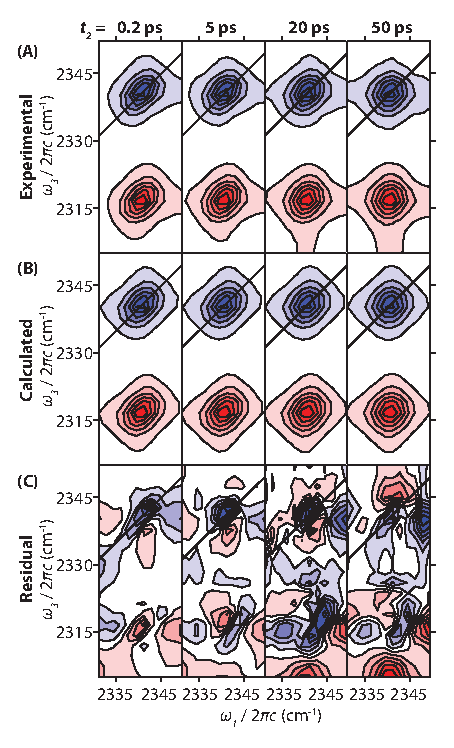
\includegraphics[scale=1.25]{./paper_01/fig8.eps}
  \caption[Example of global fitting of 2D-IR spectra]{\label{fig:TFA 2D fit}Example of global fitting of spectra. (A) Experimental 2D-IR spectra of \ce{CO2} in \ce{[Im_{4,1}]}[TFA]. (B) Calculated 2D-IR for \(\nu_3\) based on a third-order response function, which is fitted to A by optimizing the correlation time \(\tau_c\), frequency range \(\Delta\), and dephasing time \(T_2\), in addition to several other parameters (see text). (C) Residual between the experimental and calculated spectra.}
\end{figure}

\begin{table}
  \centering
  \caption[Best fit correlation function parameters, by ionic liquid]{\label{tab:2}Best fit correlation function parameters, by ionic liquid. \(\tau_c\) indicates the timescale of structural relaxation around \ce{CO2}, the inhomogeneous linewidth \(\Delta\) reflects the range of frequencies experienced by \ce{CO2} in different local environments of each ionic liquid, and the homogeneous dephasing time \(T_2\) arises from fast motions, such as librations, of \ce{CO2}.}
  \begin{tabular}{ccccc}
	\toprule
    Anion & \(\Delta\) (\si{\wavenumber}) & \(\tau_c\) (\si{\ps}) & \(T_2\) (\si{\ps}) \\
    \midrule %TODO fix math
    \ce{[PF6]-} & $2.0 \pm 0.1$ &  $104 \pm 10$ & $3.3 \pm 0.1$ \\
    \ce{[Tf2N]-} & $1.6 \pm 0.1$ &  $26 \pm 5$ & $2.8 \pm 0.1$ \\
    \ce{[TfO]-} & $1.7 \pm 0.1$ & $25 \pm 5$  &  $2.7 \pm 0.1$ \\
    \ce{[TFA]-} & $1.8 \pm 0.1$ & $40 \pm 5$ & $2.6 \pm 0.1$ \\
    \ce{[DCA]-} & $1.6 \pm 0.1$ & $13 \pm 3$ & $3.2 \pm 0.2$ \\
    \ce{[SCN]-} & $1.8 \pm 0.1$ & $16 \pm 3$ & $3.4\pm 0.1$ \\
    \bottomrule
  \end{tabular}
\end{table}

The lineshape parameters (Table~\ref{tab:2}) for \(\nu_3\), combined with insights from computational modeling of \ce{CO2}-anion-cation clusters, help to refine a physical picture of the solvation environment of \ce{CO2} in ionic liquids. The timescale of frequency fluctuation correlations (\(\tau_c\)) for \ce{CO2} varies by up to an order of magnitude between the solvents, from \SI{13(3)}{\ps} in \ce{[Im_{4,1}]}[DCA] to \SI{104(10)}{\ps} in \ce{[Im_{4,1}]}[\ce{PF6}]. The inhomogeneous width (\(\Delta\)) which is largest in \ce{PF6-} and smallest in \ce{DCA-} reflects the diversity of local environments reported by \ce{CO2} in an ionic liquid. The dephasing time (\(T_2\)), which varies from \SIrange{2.6}{3.4}{\ps}, is longer than typical dephasing times in molecular solvents.

A quantitative analysis based on lineshape theory has allowed us to determine the dynamical timescales, dephasing times, and inhomogeneous linewidths for \(\nu_3\) in the six ionic liquids studied.

\subsection{Modelling of Shoulders and Cross-Peaks}
\label{sec:shoulders_modeling}

Having quantified the change in shape of the main 2D \(\nu_3\) band, we now turn to modelling of the dynamics encoded in the diagonal shoulders and cross-peaks.

Fluctuations in the \ce{CO2} \(\nu_2\) population can be described by a thermal equilibrium between \(n\) bending modes:

\begin{equation}
  \label{eq:kinetic}
  |00^00 \rangle \overset{k_{f}}{\underset{k_{r}}\rightleftharpoons} |01^10 \rangle \cdots \overset{k''_{f}}{\underset{k''_{r}}\rightleftharpoons} |0n^l0 \rangle
\end{equation}
The rate of transition between the ground and first excited state, \(k_f\), combined with the Boltzmann distribution of states, determines the remaining rates. \(k_f\) is ultimately determined by the probability of stochastically gain a quantum of energy in a \ce{CO2} bending mode, most likely through collisions in the local environment. The first backwards rate, $k_r$, is directly analogous to the off-equilibrium vibrational energy relaxation rate.

A model that combines probabilistic fluctuations in bending mode population based on Equation \ref{eq:kinetic} with standard response function treatment is able to capture the essential physics required for such stochastic hot bands and their cross-peaks. The frequency of the \(\nu_3\) mode has two sources of variation: (1) the classical bath of intermolecular modes usually encountered in solvation dynamics and (2) the quantum bath of intramolecular vibrations to which the \(\nu_3\) band is coupled. The frequency of the \(\nu_3\) mode, $\omega(t)$ fluctuates as
\begin{equation}
  \label{eq:stochastic_frequency}
  \omega(t) = \braket{\omega} + \delta\omega_\mathrm{inter}(t) + \delta\omega_\mathrm{intra}(t).
\end{equation}
This stochastic frequency can be used as an input to standard nonlinear response function formalism. For example, the first order response function
\begin{equation}
  \label{eq:R1_1}
  R^{(1)}(t) \propto \exp{\left( -i\braket{\omega} t \right)} \times \Braket{ \exp{\left(-i\int_0^t \mathrm{d}t' \delta\omega_\mathrm{inter}(t') + \delta\omega_\mathrm{intra}(t')\right)} },
\end{equation}
can be separated into the two parts, assuming the intra- and inter-molecular modes are uncorrelated,
\begin{equation}\label{eq:R1_2}
  R^{(1)}(t) \propto \exp{\left( -i \braket{\omega} t \right)} \times \Braket{ \exp{\left( -i\int_0^t \mathrm{d}t' \delta\omega_\mathrm{inter}(t') \right)} } \times \Braket{  \exp{\left( -i\int_0^t \mathrm{d}t''\delta\omega_\mathrm{intra}(t'') \right)} }.
\end{equation}
The intermolecular component can be treated with the cumulant expansion truncated at second order
\begin{equation}
  \label{eq:R1_2b}
  R^{(1)}(t) \propto \exp{\left( -i \Braket{\omega} {t} - g(t) \right) } \times \Braket{ \exp{ \left( -i\int_0^t \mathrm{d}t''\delta\omega_\mathrm{intra}(t'') \right)} }.
\end{equation}
where \(g(t)\) is the lineshape function. The extension to third-order response functions is straightforward.

We performed a stochastic simulation in which an ensemble of trajectories was generated by allowing probabilistic instantaneous transitions between the ground and excited states of the \(\nu_2\), with upward and downward rates consistent with the equilibrium populations. These transitions were allowed to happen at any point in the simulation, including during the coherence times.

The simulated lineshape is sensitive to the rate of thermal fluctuations in \(\nu_2\). By tuning the rate constant \(k_f\) of stochastic fluctuation from the ground state into the first excited state and enforcing detailed balance to preserve equilibrium, we can control (1) whether or not diagonal shoulders will appear, and (2) the kinetics of cross-peak formation. In the limit of fast fluctuations, there are no clearly observed shoulders or cross-peaks, as all three peaks coalesce into a single band. In the limit of slow fluctuations, there are clearly defined shoulders, which persist throughout the experimental timescale, and cross-peaks do not grow into the spectrum. In an intermediate regime, we are able to reproduce both the lineshape and kinetics (Figures~\ref{fig:sim spect} and \ref{fig:shoulder kinetics}) seen in the relative intensities of the first shoulder and the cross-peaks between it and the main peak  as functions of population time.

\begin{figure}
  \centering
  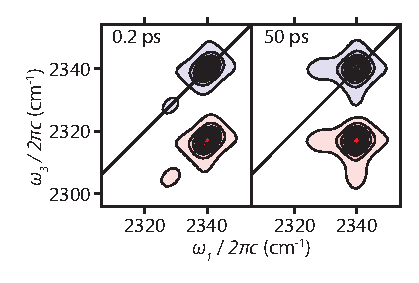
\includegraphics[scale=1.10]{./paper_01/fig9.eps}
  \caption[Stochastic simulation spectrum]{\label{fig:sim spect}Calculated spectrum of \ce{CO2} in \ce{[Im_{4,1}]}[TFA] at $t_2 =$ \SIlist[list-units = single]{0.2;50}{\ps}. Spectra are based on a stochastic simulation that allows the bending mode of a particular oscillator to fluctuate over the course of the experiment (while preserving a Boltzmann distribution). The lineshape as a function of \(t_2\) closely approximates the lineshape of the main peak (1a and 2a), first diagonal shoulder (1b and 2b), and cross-peaks (1b,a; 2a,b and 2b,a) in the experimental spectra (Figure~{\ref{fig:example 2D}}).}
\end{figure}

The microscopic rate constant ($k_{\mathrm{up}}$) for \ce{CO2} bending mode fluctuations in \ce{[Im_{4,1}][TfO]}, from the Monte Carlo simulations is estimated to be $k_{\mathrm{up}} =$ \SI{2.5(1)}{\per\ns}. The corresponding down rate, which is analogous to the vibrational relaxation rate in off-equilibrium pump-probe experiments, is estimated to be $k_{\mathrm{down}} =$\SI{30(12)}{\per\ns}. The kinetic Monte Carlo simulations include the non-equilibrium pumping that was explained by Fayer et al. \cite{Giammanco2016}. Their pump-probe measurements showed an increase in the ground state bleach band due to differences in transition dipole moment between the ground state $|000\rangle$ and the `hot' band $|01^10\rangle$ transition dipole moments. The 2D measurement resolves the excitation frequency, so those dynamics are visible as a separate cross-peaks, where the pump-probe measurement observes the sum of the two peaks (the projection of the spectrum onto the \(\omega_3\)-axis). The main ground state bleach decays with bending mode exchange and the cross-peak grows. If the dipoles of the two states are the same these two terms cancel in the pump-probe measurement; however, the differences in dipole lead to effective rises in the pump-probe ground state bleach signal.

\section{\texorpdfstring{\caps{Molecular Interpretation}}{Molecular Interpretation}}
\label{sec:anions_interpretation}

The resulting molecular picture is that the slower dynamics of the ionic liquid solvent \textit{gate} \ce{CO2}'s dynamics in solution. The slow timescale (\(\tau_c\)) arises from structural relaxation of the solvent around \ce{CO2}, and corresponds to the breakup of local ion shells. Until this liberating event, \ce{CO2} is caged in a relatively well-ordered local environment. Librational and other fast motions only sample a narrow range of instantaneous frequencies, but the variation in instantaneous frequency between different local environments gives rise to the inhomogeneous linewidth.

We assign the inhomogeneous width, \(\Delta\), to the interactions of the \ce{CO2} with its local ion cage. Because charge transfer drives the distortion of the \ce{CO2} geometry, and the geometry determines the \(\nu_3\) frequency, \(\Delta\) reports the range of local structural motifs that the \ce{CO2} can sample.
This range varies from \SI{2}{\wavenumber} in \ce{[PF6]} to \SI{1.6}{\wavenumber} in [DCA]  (a 20\% decrease). \(\Delta\) is also not strongly correlated to the average frequency shift or other structural parameters, and so we attribute it to the range of structures in the condensed phase.

The inhomogeneous linewidth of \ce{CO2} is the narrowest of the IR probes in recent 2D-IR experiments. Thiocyanate, \ce{SCN-}, has a total inhomogeneous linewidth \(\Delta_\mathrm{total} \sim \SI{8}{\wavenumber}\);\cite{Ren2014} heavy water, HOD, \(\Delta_\mathrm{total} \sim \SI{5}{\wavenumber}\);~\cite{wongJPCB-13} and \ce{CO2} \(\Delta_\mathrm{total} \sim \SI{2}{\wavenumber}\). This trend reflects the strength of the coupling of the vibrational chromophore to its environment. The \ce{SCN-} anion is directly integrated into the ion network and hydrogen-bonded to the imidazolium cation through the 2-position. HOD interacts more weakly with the ionic liquid. It associates primarily with the anion, but it is sensitive to the electric field projected on the OH (or OD) bond axis. Because HOD is dipolar, it still experiences relatively large frequency fluctuations. \ce{CO2} is even more weakly still coupled to its environment. \ce{CO2}, which has a quadrupole moment and no dipole moment, is even less influenced by the local electric fields and is sensitive to the more chemical nature of the \ce{CO2}-anion-cation interaction.

Similarly, we assign the spectral diffusion time, \(\tau_c\), to a local ion cage's lifetime around \ce{CO2}. The observed timescale reflects the time for the ion cage around \ce{CO2} to break up and permit \ce{CO2} to move to a novel local environment. This interpretation is consistent with previous computational work which indicate that the ionic liquid solvent reorients spontaneously to accommodate \ce{CO2} in well-defined locations in the ionic liquid,~\cite{Huang2005} and with NMR studies showing a well-defined angular distribution of \ce{CO2} around the cation.~\cite{Corvo2013}

The bulk viscosity, \(\eta\), serves as a proxy for this rate of diffusion which we can compare across the anions. Of course, small, neutral molecules like \ce{CO2} experience less friction from the solvent than the viscosity implies.\cite{Kaintz2013,Kaintz2014-corr} Nevertheless, the linear correlation of bulk viscosity and \(\tau_c\) (\(R^2 = 0.82\))  supports our assignment (Figure~\ref{fig:visc correlation}). This correlation further suggests that the motion of the smaller, more mobile \ce{CO2} through the ionic liquid is gated by the motion of the solvent ions.

\begin{figure}
  \centering
  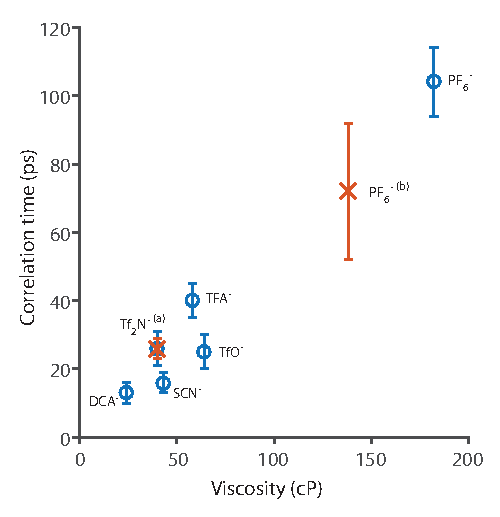
\includegraphics[scale=1.25]{./paper_01/fig10.eps}
  \caption[\texorpdfstring{\(\tau_c\)}{tau(c)}-viscosity correlation with differing ionic liquid anion]{\label{fig:visc correlation}Correlation time, \(\tau_c\), compared with viscosity for the 1-butyl-3-methylimidazolium ionic liquid solvent. Data points marked with an `O' are from \ce{CO2} in this work, while those marked `X' are correlation times from other works (a) \ce{SCN-} in \ce{[Im_{4,1}][Tf2N]},\cite{Ren2014} (b) HOD in \ce{[Im_{4,1}][PF6]},\cite{wongJPCB-13} with ionic liquid viscosity scaled to account for water content.\cite{Li2007}  Literature values for viscosity were used for all ionic liquids.\cite{Tokuda2006a,Domanska2012,Sanchez2009}}
\end{figure}

\ce{CO2} has a Lewis acid-base interaction with the anion of the ionic liquid. Isolated water has possible hydrogen bonds with both the anion and the cation. \ce{SCN-} has a strong electrostatic attraction to the cation. Thus, all three chromophores have different specific interactions with their ionic liquid solvent. Nevertheless, the correlation times seen in 2D-IR studies of \ce{[SCN]-} in \ce{[Im_{4,1}][Tf2N]}\cite{Ren2014} and \ce{D2O}/\ce{HOD} in \ce{[Im_{4,1}][PF6]}\cite{wongJPCB-13} follow the same viscosity trend, when you account for the expected \(\sim 25\)\% decrease in the viscosity of \ce{[Im_{4,1}][PF6]} with \(\chi_{\ce{H2O}} \approx 0.04\).\cite{Li2007} This fact suggests that each of these chromophores is reporting on the local diffusive motion of the surrounding solvent, despite the fact that \ce{SCN-}, water, and \ce{CO2} have different specific interactions with the ions in their solvation shells.

Furthermore, recent MD simulations suggest a direct relationship between ion cage lifetime and bulk transport properties such as self-diffusivity and conductivity.\cite{Zhang2015b} While diffusivity of \ce{CO2} and self-diffusivity of an ionic liquid are not identical parameters, the dynamics reported by \ce{CO2} and \ce{[SCN]-}\cite{Ren2014} in \ce{[Im_{4,1}][Tf2N]} are nearly identical, and both have been related to ion cage lifetime. Thus, it is reasonable to speculate that \ce{CO2} mass transport in these ionic liquids may depend also depend on ion cage lifetime. In this case, the correlation times reported could provide an avenue to directly address the molecular mechanism of \ce{CO2} mass transport in ionic liquids, and might even give insight into other transport properties such as self-diffusivity and conductivity.

The homogeneous dephasing time, \(T_2\), depends on both the timescale of fast motions for \ce{CO2}, $\tau_H$, and on the frequency range experienced during those motions, \(\Delta_H\) ($T_{2} = \left( {\Delta}_H^{2}\tau_H \right)^{-1}$). Experimentally, it is impossible to disentangle these two contributions, but the dephasing time (\(\sim \SI{3}{\ps}\)) is significantly longer than that seen for either HOD (\(\sim \SI{1}{\ps}\)) or \ce{SCN-} (\(\sim \SI{1.4}{\ps}\)) in ionic liquids. Thus, either \ce{CO2} samples a relatively narrow frequency range during its homogeneous motions, or the those motions are particularly fast. Based on the small inhomogeneous linewidth, \(\Delta\), and the fact that \ce{CO2} is a small molecule whose moment of inertia (and consequently, the timescale for fast motions such as librations) is unchanged between ionic liquids and molecular solvents, it seems reasonable that the long dephasing time results from a narrow frequency range in a well-defined local environment, rather than a decrease in solvent interactions that slow the molecule.

Furthermore, the computational results show that, in gas phase clusters, \ce{CO2} bends and adopts a distorted equilibrium geometry. In condensed phase dynamics, transitioning from a linear to a bent geometry could be one method of populating an excited state bending mode, and could have a direct impact on \(k_f\), the rate of bending mode transitions. In principle, the spectral diffusion rate should influence the rate of transition between equilibrium geometries, and thus drive excitation and de-excitation of bending modes. Since we are able to model \(k_f\) based on equilibrium measurements, a systematic study of ionic liquids with different spectral diffusion rates could experimentally elucidate to how the motions of the solvent around a small molecule influence stochastic fluctuations in bending mode population.

These molecular mechanisms can be both tested and clarified by the comparison of these results to simulation. Frequency mapping techniques, combined with classical molecular dynamics simulations can be used to calculate the IR absorption spectrum and the spectral diffusion of modes of interest for small molecules such as water,\cite{steinelCPL-04,Asbury2004,Corcelli2004} nitriles and thiocyanate,\cite{Choi2008,Lindquist2008} and azides\cite{liJPC-06,Li2006} in molecular solvents. More recently these methods have been expanded to explore isolated water in imidazolium ionic liquid solvents\cite{Terranova2014}, with good agreement with experiment.\cite{wongJPCB-13} Similar approaches for \ce{CO2} could verify the molecular mechanism of \ce{CO2} solvation in ionic liquids. It is likely, given the calculated dependence of \(\nu_3\) on \ce{CO2} geometry, that any molecular dynamics simulation would need to account for the geometrical distortion of the \ce{CO2} due to charge transfer, either directly via on-the-fly QM calculations, or with a classical proxy that indirectly accounts for these effects.

These initial studies utilized imidazolium-based ionic liquids because they are commercially available, are ``archetypal,'' and are relatively well-characterized; thus, they provide a good initial platform on which to develop spectroscopic methods. Many ionic liquids of interest, however, involve either novel classes of anions and cations or chemical modification of existing ionic liquids. The changes in solvent structure and dynamics that result from such modifications are generally \textit{not} well-understood. This type of spectroscopy can provide valuable molecular insights into how and why chemical modification of ionic liquids determines bulk properties of interest, especially \ce{CO2} uptake and local ion mobility (which is related to viscosity and conductivity). Chemisorbing ionic liquids are also of interest, especially for carbon capture applications, and many (1) have an initial physisorption step, and (2) have an equilibrium between physisorbed and chemisorbed (reacted) \ce{CO2}. These types of studies could help to elucidate the molecular mechanisms of the equilibrium between \ce{CO2} in its free and bound forms.

\section{\texorpdfstring{\caps{Conclusions}}{Conclusions}}
\label{sec:anions_conclusions}

We have demonstrated that the \ce{CO2} \(\nu_3\) mode can act as a probe of local structure and dynamics in imidazolium ionic liquids. This method has potential application to the analysis of structure and dynamics in ionic liquids being developed for \ce{CO2} capture.

The \(\nu_3\) frequency is sensitive to the timescale of local structural relaxation in ionic liquids. The timescale of this relaxation, \(\tau_c\) is determined by spectral modelling using a third-order response function formalism, with a Bloch-Kubo lineshape. For the imidazolium ionic liquids studied, \(\tau_c\) varies by as much as an order of magnitude between solvents, and correlates with the viscosity of the ionic liquids. The molecular mechanism posited for this timescale is the breakup of local ion cages around the \ce{CO2}.

Computational studies aid understanding the origin of the \(\nu_3\) center frequency shifts in different imidazolium ionic liquids and suggest that geometrical distortion of the \ce{CO2}, driven by charge transfer from the anion into virtual orbitals of \ce{CO2} and from occupied orbitals of \ce{CO2} into virtual orbitals of the cation. A simple one exciton Hamiltonian is able to reproduce the scaled harmonic frequencies with an RMS error of \SI{1.2}{\wavenumber} by accounting for dependence of average frequency, \(\alpha\), on total bond length, \(L\), and the coupling constant, \(\beta\), on magnitude of the angular distortion of \ce{CO2}, \(\theta\).

Anharmonic coupling of \(\nu_2\) and \(\nu_3\) allows thermal fluctuations of \(\nu_2\) population to stochastically shift the \ce{CO2} \(\nu_3\) by units of \SI{-12}{\wavenumber} (the coupling constant), and cause the appearance of a shoulder and dynamic cross-peaks on the 2D spectrum. Modelling of the stochastic bending mode population over the timescale of the experiment gives an estimate of the rate of excitation and de-excitation of bending mode population in the condensed phase at thermal equilibrium, estimated to be \(k_{f} = \SI{2.5 \pm 1}{\per\ns}\) and $k_r = 30\pm12$~\si{\per\ns}. Additional spectral features (the ``second shoulder'' and apparent ``cross-peak'' 1c) arise from fifth-order signal.

The molecular picture that arises from this work is one in which imidazolium ionic liquids solvate \ce{CO2} in well-defined local environments. The interactions of \ce{CO2} with its solvent are dominated by local interactions with its nearest neighbor anion and cation. The picosecond dynamics of \ce{CO2} are gated by the slower local diffusive motions of the anion and cation, whose translations and rotations are hindered due to electrostatic friction from surrounding ions, and potentially due to dispersive interactions between nanosegregated alkyl chains.

The methods and analysis developed in this work describe \ce{CO2} in imidazolium ionic liquids. We expect that they will be transferable, however, to broad classes of materials, such as polymers or metal-organic frameworks, as well as to other ionic liquids.

\section{\texorpdfstring{\caps{Supporting Information}}{Supporting Information}}
\label{paper_01:sec:SI}

\subsection{Comparison of Global Fitting with Center Line Slope}
\label{anionSI_CLS}

For the center line slope method, we fit the signal size as a function of final frequency (\(\omega_3\)) with two Gaussians with opposite signs for each initial frequency (\(\omega_1\)) data point. The resolved positions of the Gaussians of the 0 to 1 transition peak are considered the center points. The center line slope is determined by  fitting the center points linearly as a function of \(\omega_1\). Estimated errors are propagated accordingly.

The resulting center line slope is fitted to a biexponential decay as a function of \(t_2\)
\begin{equation}
c_2 = \sum_{i=1}^2 a_i \exp{\left( -t_2/\tau_i \right)}
\end{equation}
with the resulting parameters for \ce{CO2} \(\nu_3\) in \ce{[Im_{4,1}][TFA]}: \(a = 0.09 \pm 0.04, \tau_1 = 2.1 \pm 2.1 \si{\ps}, b = 0.35 \pm 0.04, \tau_2 = 35 \pm 5 \si{\ps}\).

\begin{figure}[h]
  \centering
  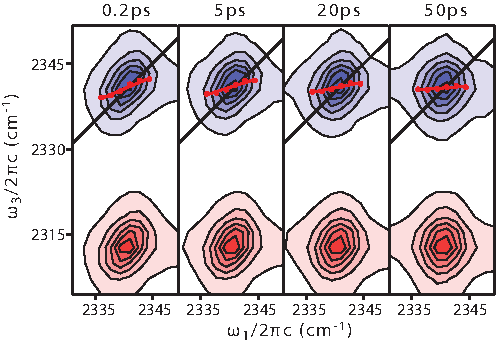
\includegraphics[scale=0.8]{./paper_01/CLS_BMIMTFA.pdf}
  \caption[CLS overlaid on 2D-IR spectrum]{CLS overlaid on the 2D spectrum of \ce{CO2} in \ce{[Im_{4,1}][TFA]}}
\end{figure}

\begin{figure}[h]
  \centering
  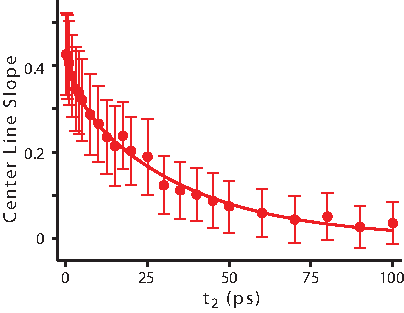
\includegraphics[scale=1]{./paper_01/CLS_fit_BMIMTFA.pdf}
  \caption[CLS fitting of 2D-IR spectrum]{CLS fitting of \ce{CO2} \(\nu_3\) 2D spectrum from \ce{[Im_{4,1}][TFA]}}
\end{figure}

\subsection{2D IR Spectra}
\label{anionSI_2D}

\begin{figure}[h]
  \centering
  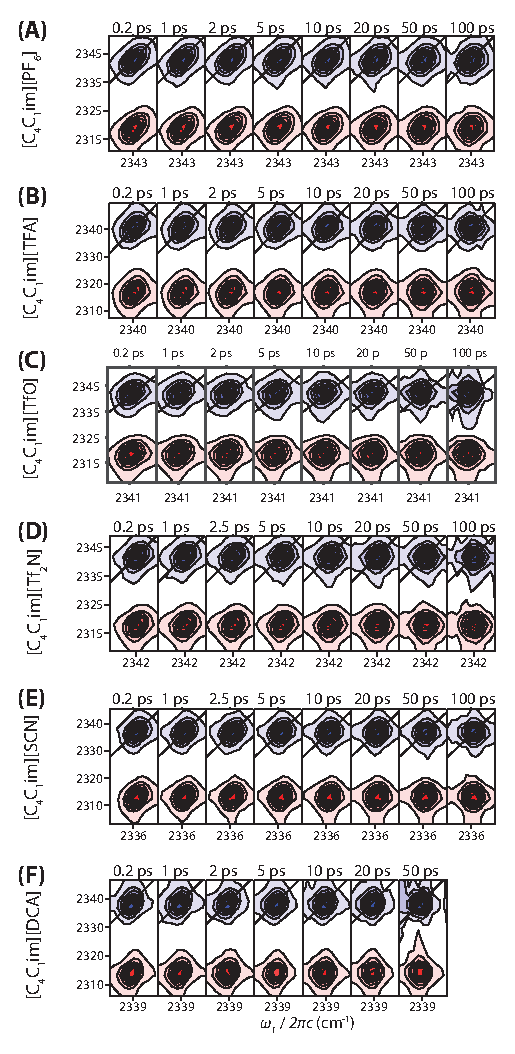
\includegraphics[scale=1.0]{./paper_01/all_2d.eps}
  \caption{2D-IR spectra of \ce{CO2} \(\nu_3\) in \ce{[Im_{4,1}+]} (A) \ce{[PF6]-}, (B) \ce{[TFA]-}, (C) \ce{[TfO]-}, (D) \ce{[Tf2N]-}, (E) \ce{[SCN]-}, and (F) \ce{[DCA]-}, showing the range of timescales for spectral diffusion in \(\nu_3\).}
  \label{paper_01:fig:SI_all_2D}
\end{figure}

\subsection{Computational Results}
\label{anionSI_comp}
%Geometries optimized disallowing charge transfer.
In tables~\ref{paper_01:tab:S1}~and~\ref{paper_01:tab:S2}, `\(\nu_1\)' is the frequency of the symmetric stretching mode of \ce{CO2}, and `\(\nu_3\)' is the frequency of the antisymmetric stretching mode of \ce{CO2}. \(\alpha\) is the average of the two normal mode frequencies, \(\alpha = (\omega_\mathrm{s} + \omega_\mathrm{a})/2\). \(\beta\) is the coupling constant, or the difference of the two local mode frequencies, \(\beta = (\omega_\mathrm{s} - \omega_\mathrm{a})/2\).

`CT: \ce{CO2} to IL` is the amount of charge transferred from the \ce{CO2} into the ionic liquid components, `CT: IL to \ce{CO2}` is the amount of charge transferred from the ionic liquid components into the \ce{CO2}, and `CT: net` is the net charge transferred into the \ce{CO2}.

`geom: angle' is the \ce{CO2} \ce{O--C--O} angle, and `geom: \(\theta\)' is the deviation of the angle from \ang{180}. `geom: \(l_1\)' and `geom: \(l_2\)' are the bond lengths of the two \ce{C-O} bonds, `geom: \(l_2 - l_1\)' is the difference between the two bonds lengths, and `geom: \(L\)` is the sum of the two bond lengths. `geom: \ce{O_{12}}' is the through-space oxygen-oxygen distance in \ce{CO2}.

\begin{landscape}
  \begin{table}
    \centering
    % \resizebox{1\textwidth}{!}{
    \caption{\texorpdfstring{\cotil}{Carbon dioxide-IL} geometries optimized allowing charge transfer}
    \label{paper_01:tab:S1}
    \small
    \tabcolsep=0.11cm
    \begin{tabular}{rcccccccccc}
      \hline
      & Free \ce{CO2} & Cation & \ce{BF4} & \ce{DCA} & \ce{PF6} & \ce{SCN} & \ce{TFA} & \ce{Tf2N} & \ce{TfO} \\
      \hline
      \(\nu_1\) (\si{\wavenumber}) & 1371.93 & 1372.12 & 1372.96 & 1370.71 & 1373.95 & 1370.35 & 1371.68 & 1372.88 & 1371.14 \\
      \(\nu_3\) (\si{\wavenumber}) & 2436.1 & 2443.07 & 2434.71 & 2430.85 & 2437.48 & 2430.27 & 2429.81 & 2437.74 & 2433.89 \\
      \(\beta\) (\si{\wavenumber}) & -532.085 & -535.475 & -530.875 & -530.07 & -531.765 & -529.96 & -529.065 & -532.43 & -531.375 \\
      \(\alpha\) (\si{\wavenumber}) & 1904.015 & 1907.595 & 1903.835 & 1900.7 & 1905.715 & 1900.31 & 1900.745 & 1905.31 & 1902.515 \\
      \hline
      CT: \ce{CO2} to IL (\si{\milli\elementarycharge}) & 0 & 2.251 & 1.264 & 2.259 & 1.012 & 1.323 & 1.618 & 1.603 & 2.339 \\
      CT: IL to \ce{CO2} (\si{\milli\elementarycharge}) & 0 & 0.079 & 4.558 & 3.376 & 3.336 & 3.317 & 5.131 & 2.493 & 3.009 \\
      CT: net (\si{\milli\elementarycharge}) & 0 & -2.172 & 3.294 & 1.117 & 2.324 & 1.994 & 3.513 & 0.89 & 0.67 \\
      \hline
      geom: angle (\si{\degree}) & 179.96 & 179.93 & 175.49 & 175.01 & 176.21 & 175.65 & 174.78 & 177.36 & 175.99 \\
      geom: \(\theta\) (\si{\degree}) & 0.042 & 0.07 & 4.51 & 4.99 & 3.79 & 4.35 & 5.22 & 2.64 & 4.01 \\
      geom: \(l_2 - l_1\) (\si{\angstrom}) & \num{1.9e-7} & 0.015 & 0.0087 & 0.011 & 0.0071 & 0.0089 & 0.0076 & 0.0076 & 0.011 \\
      geom: \(l_1\) (\si{\angstrom}) & 1.169 & 1.176 & 1.174 & 1.175 & 1.173 & 1.165 & 1.173 & 1.165 & 1.175 \\
      geom: \(l_2\) (\si{\angstrom}) & 1.169 & 1.161 & 1.165 & 1.164 & 1.165 & 1.174 & 1.166 & 1.173 & 1.164 \\
      geom: \ce{O_{12}}  (\si{\angstrom}) & 2.338 & 2.337 & 2.337 & 2.337 & 2.337 & 2.338 & 2.337 & 2.337 & 2.337 \\
      geom: \(L\) (\si{\angstrom}) & 2.338 & 2.337 & 2.338 & 2.339 & 2.338 & 2.339 & 2.339 & 2.338 & 2.339 \\
    \end{tabular}%}
    \normalsize
  \end{table}


  \begin{table}
    \centering
    % \resizebox{1\textwidth}{!}{
    \caption{\texorpdfstring{\cotil}{Carbon dioxide-IL} geometries optimized without allowing charge transfer}
    \label{paper_01:tab:S2}
    \small
    \tabcolsep=0.11cm
    \begin{tabular}{rcccccccccc}
      \hline
      & Free \ce{CO2} & Cation & \ce{BF4} & \ce{DCA} & \ce{PF6} & \ce{SCN} & \ce{TFA} & \ce{Tf2N} & \ce{TfO} \\
      \hline
      \(\nu_1\) (\si{\wavenumber}) & 1371.93 & 1371.47 & 1373.31 & 1373.44 & 1373.33 & 1373.14 & 1373.65 & 1373.06 & 1373.45 \\
      \(\nu_3\) (\si{\wavenumber}) & 2436.1 & 2439.86 & 2438.56 & 2439.1 & 2438.47 & 2438.78 & 2438.39 & 2438.767 & 2439.37 \\
      \(\beta\) (\si{\wavenumber}) & -532.085 & -534.195 & -532.625 & -532.83 & -532.57 & -532.82 & -532.37 & -532.85 & -532.96 \\
      \(\alpha\) (\si{\wavenumber}) & 1904.015 & 1905.665 & 1905.935 & 1906.27 & 1905.9 & 1905.96 & 1906.0271905.91 & 1906.41 \\
      \hline
      CT: \ce{CO2} to IL (\si{\milli\elementarycharge}) & 0 & 1.743 & 1.038 & 1.836 & 1.154 & 1.302 & 1.023 & 1.246 & 1.941 \\
      CT: IL to \ce{CO2} (\si{\milli\elementarycharge}) & 0 & 0.039 & 3.053 & 2.266 & 2.221 & 1.64 & 2.916 & 1.274 & 2.048 \\
      CT: net (\si{\milli\elementarycharge}) & 0 & -1.704 & 2.015 & 0.43 & 1.067 & 0.338 & 1.893 & 0.028 & 0.107 \\
      \hline
      geom: angle (\si{\degree}) & 179.96 & 179.97 & 177.30 & 177.29 & 177.58 & 177.78 & 178.30 & 177.19 & 177.39 \\
      geom: \(\theta\) (\si{\degree}) & 0.04 & 0.03 & 2.70 & 2.70 & 2.42 & 2.22 & 1.70 & 2.81 & 2.61 \\
      geom: \(l_2 - l_1\) (\si{\angstrom}) & $1.9\times 10^{-7}$ & 0.012 & 0.008 & 0.008 & 0.007 & 0.008 & 0.007 & 0.007 & 0.009 \\
      geom: \(l_1\) (\si{\angstrom}) & 1.169 & 1.175 & 1.173 & 1.173 & 1.172 & 1.165 & 1.166 & 1.172 & 1.173 \\
      geom: \(l_2\) (\si{\angstrom}) & 1.169 & 1.163 & 1.165 & 1.165 & 1.166 & 1.173 & 1.172 & 1.166 & 1.165 \\
      geom: \ce{O_{12}} (\si{\angstrom}) & 2.338 & 2.338 & 2.337 & 2.337 & 2.337 & 2.337 & 2.338 & 2.337 & 2.337 \\
      geom: \(L\) (\si{\angstrom}) & 2.338 & 2.338 & 2.338 & 2.338 & 2.338 & 2.338 & 2.338 & 2.338 & 2.338 \\
    \end{tabular}%}
    \normalsize
  \end{table}
\end{landscape}

\chapter[\ce{CO2}-IL Cluster Model Validation]{Modeling Carbon Dioxide Vibrational Frequencies in Ionic Liquids: I. \textit{Ab Initio} Calculations}
\label{ch:paper_02}

The text in this chapter has been adapted from \fullcite{Berquist2017}. The author's contribution to the work included performing all quantum chemical calculations and analyses (excepting those for DVR), designing the charge transfer mechanism and counterpoise correction analyses, writing those respective parts of the manuscript, and editing/revising the remainder.

\section{\texorpdfstring{\caps{Summary}}{Summary}}
\label{paper_02:sec:summary}

This work elucidates the molecular binding mechanism of \ce{CO2} in \ce{[C4C1im][PF6]} ionic liquid (IL) and its interplay with the \ce{CO2} asymmetric stretch frequency \(\nu_{3}\), and establishes computational protocols for the reliable construction of spectroscopic maps for simulating ultrafast 2D-IR data of \ce{CO2} solvated in ILs. While charge transfer drives the static frequency shift between \emph{different} ionic liquids [\emph{J. Chem. Phys.} \textbf{142}, 212425 (2015)], we find here that electrostatic and Pauli repulsion effects dominate the dynamical frequency shift between different geometries sampled from the finite-temperature dynamics within a single ionic liquid. This finding is also surprising because dispersion interactions dominate the \cotil interaction energies, but are comparably constant across different geometries. An important practical consequence of this finding is that density functional theory is expected to be sufficiently accurate for constructing potential energy surfaces for \ce{CO2} in \ce{[C4C1im][PF6]}, as needed for accurate anharmonic calculations to construct a reliable spectroscopic map. Similarly, we established appropriate computational and chemical models for treating the extended solvent environment. We found that a QM/MM treatment including at least \num{2} cation-ion pairs at the QM level and at least \num{32} pairs at the MM level is necessary to converge vibrational frequencies to within \SI{1}{\wavenumber}. Using these insights, this work identifies a computational protocol as well as a chemical model necessary to construct accurate spectroscopic maps from first principles.

\section{\texorpdfstring{\caps{Introduction}}{Introduction}}
\label{paper_02:sec:I}

Capturing anthropogenic \ce{CO2} before its release into the atmosphere is a pressing need, and most methods will require the development of novel materials, such as metal-organic frameworks, polymers, or ionic liquids (ILs).\cite{sumidaCR-12,Du2011,Dawson2011,baraACR-10,seoJPCB-14,DAlessandro2010} Understanding how to control the interactions between \ce{CO2} and its condensed-phase environment is a key to achieving efficient carbon capture and sequestration\cite{Corvo2015,Hayes2015,seoJPCB-14,gurkanJPCL-10} and to developing routes toward potentially transforming \ce{CO2} into value-added chemicals including fuels.\cite{Grice2015,Rosen2011,Kumar2012} To rationally develop such technologies, a molecular level understanding of the \ce{CO2}-sorbent interactions, structures and dynamics is necessary.

In a previous paper\cite{Brinzer2015}, some of us established that \ce{CO2}'s asymmetric vibrational stretch mode (\(\nu_{3}\)) can be used to effectively probe the structure and dynamics of \ce{CO2} dissolved in ILs. Using a combination of ultrafast two-dimensional infrared (2D-IR) spectroscopy and computational modeling, we determined structural candidates for the immediate \ce{CO2} solvent environments whose vibrational solvation shifts were consistent between experiment and theory. Experimentally, the timescales of structural reorganization relative to the \ce{CO2} molecule were correlated to the bulk viscosity. This experimental correlation between molecular property (solvation timescales) and bulk property (viscosity) suggests that \ce{CO2} motions are gated by the same motions that lead to bulk diffusion. Molecular models are needed, however, to establish physical explanations for the correlation.

\ce{CO2} solvation in ionic liquids gives rise to several interesting and challenging effects that are worth exploring thoroughly, taking both computational methodology and the chemical picture into account. Our previous work suggested that charge transfer (CT) between \ce{CO2} and the IL dominates the differentiation of the calculated vibrational signatures between different ionic liquids. Understanding the strength and nature of intermolecular interactions between \ce{CO2} and its IL solvent fundamentally shapes our model of the \cotil interaction. Investigating \cotil interactions will thus deepen our understanding of the mechanism of \ce{CO2} solubility in ionic liquids, and even of (de)activation of \ce{CO2} for catalytic reductions. Interestingly, the asymmetric stretch frequency of \ce{CO2} encodes the strength of intermolecular interactions as they are manifested in the molecular geometry of \ce{CO2} interacting with the surrounding IL. In other words, one can determine the correct vibrational frequency shift for \ce{CO2} from the distortion of the \ce{CO2} geometry, but correctly determining the \ce{CO2} geometry requires an understanding of intermolecular interactions between \ce{CO2} and the IL solvent. These effects must be considered in the development of more reliable force fields that describe \cotil solvation, and of empirical structure-spectra maps used for comparing MD results with results from ultrafast spectroscopies.

This publication is first in a series aiming to unravel the physics underlying \cotil interactions as probed via vibrational spectroscopy and to develop a spectroscopic map to facilitate simulation of these spectra. \emph{The central point of the present publication is to establish a more refined picture of intermolecular interactions and their correlations with vibrational shifts by improving both the computational approach and the chemical model as described below.} Some of the results from this publication inform the method choices for the subsequent paper in the series, where we develop and validate a spectroscopic map enabling one to reliably predict both the position and the width of the \ce{CO2} asymmetric vibrational peak within classical MD simulations.\cite{Daly2016}

In this manuscript, we address the critical challenges needed to generalize our previous work. The key issues are: treating the condensed phase environment, testing the dependence on the electronic structure theory method and basis set, and addressing anharmonic effects.

First, we extend our previous results by analyzing both the convergence and stability of the calculations with respect to the computational approach. Our absolutely localized molecular orbital (ALMO) calculations\cite{Khaliullin2006,Khaliullin2007,Khaliullin2008} evaluated the impact of CT and other chemically intuitive components in the calculation of spectral signatures by using the modest B3LYP/6-31G(d,p) level of theory. Like most decomposition approaches, the ALMO results are expected to show some dependence on the underlying density functional approximation; in particular, it is known that the predicted amount of charge transfer depends on the amount of self-interaction error (SIE) present and the resulting (spurious) delocalization\cite{Ramos-Cordoba2011}. As a result, non-SIE corrected functionals are expected to overestimate the amount of CT, whereas the SIE-free Hartree\textendash{}Fock approach can be used to estimate a lower bound for CT effects. Likewise, one can expect the CT contribution to depend on the basis set diffuseness, since the ALMO definition of CT is closely linked to the penetration of basis functions between different fragments. Thus, one goal of the present study is to quantify the method and basis set dependence of the calculated vibrational shifts and their effect on CT.

Although our previous density functional theory (DFT) calculations provided excellent agreement of predicted vibrational solvation shifts compared to experiment, these employed a minimalistic gas-phase cluster model consisting of only one \ce{CO2} molecule together with a single cation/anion pair. Here we investigate the convergence of results with the size of the surrounding solvent shell both using a hybrid quantum mechanics molecular mechanics (QM/MM) approach with up to \num{195} atoms (\num{6} molecular ion pairs) in the QM region and up to \num{8192} solvent atoms (\num{256} molecular ion pairs) using classical point charges. In addition, we aim to assess the impact of solvent disorder by investigating different solvent geometries based on \num{85} statistically uncorrelated (\(R^2 = 0.0004\) for DVR-based vibrational frequency of snapshot \(N\) to vibrational frequency of snapshot \(N+1\)) snapshots sampled from a classical MD simulation (see paper II\cite{Daly2016} for details). We use 1-butyl-3-methylimidazolium hexafluorophosphate (\ce{[C4C1im][PF6]}) as a model IL in our calculations.

We will further analyze the impact of anharmonic effects, which we neglected in our previous (harmonic) calculations and which are necessary for a fair comparison to experiment. Here, anharmonic vibrational frequencies are obtained using the discrete variable representation (DVR) approach. The DVR method numerically solves the vibrational Schr\"{}odinger equation using a calculation of the \ce{CO2} stretch potential energy surface, resulting in vibrational frequencies that include anharmonicity to all orders. An additional advantage of DVR is that it can be applied rigorously to systems at non-equilibrium geometries, which allows us to include the disorder introduced by temperature for comparison with experiments carried out at temperatures above absolute zero.

The energy decomposition approaches we use add new and valuable physical insight into the origin of the vibrational frequency shifts. Many groups have used QM/MM approaches to estimate the condensed phase effects of a solvent on the transition energies of a chromophore, which provide a rich interpretation of the experiments\cite{choiJCP-08,Lindquist2008,Terranova2014,liJPC-06,Schmidt2008}. Nevertheless, the interpretation for why the environment shifts the transition frequencies is difficult because many effects simultaneously determine the transition frequencies. The ALMO and symmetry-adapted perturbation theory (SAPT) energy decomposition approaches can separate the interactions of the vibrational chromophore with its environments into meaningful components allowing us to develop an empirical spectroscopic map and also understand its physical origins.

The paper is organized as follows. In section~\ref{paper_02:sec:II}, we give a detailed account of the computational approaches used, including DFT calculations and DVR vibrational frequency calculations. In section~\ref{paper_02:sec:III}, we analyze the dependence of the calculated \ce{CO2} vibrational frequencies on the computational approach and the chemical model. For the computational approach, we quantify both the impacts of the electronic structure method (density functional and basis set) as well as the inclusion of anharmonic effects via the DVR approach. We analyze the dependence on the chemical model by comparing our previous gas-phase cluster calculations with results obtained for extended solvent boxes both at the classical point charge and the hybrid quantum mechanics/molecular mechanics (QM/MM) level, where structures are sampled from extensive molecular dynamics (MD) simulations (details of the MD simulations will be discussed in a follow-up paper\cite{Daly2016}). This way, we aim to include the most important effects of solvent electrostatics, exchange-repulsion, and solvent disorder. In section~\ref{paper_02:sec:IV} we present concluding remarks and an outlook for future research.

\section{\texorpdfstring{\caps{Computational Methods}}{Computational Methods}}
\label{paper_02:sec:II}

\subsection{Methods and Basis Sets}
\label{paper_02:ssec:IIA}

Similar to our previous work\cite{Brinzer2015}, we choose gas-phase clusters consisting of one \ce{[C4C1im][PF6]} ion pair with \ce{CO2} to quantify the effects of quantum chemical method and basis set on the quantum mechanically calculated harmonic frequencies. For methods, we employ the BLYP\cite{Becke1988,Lee1988} generalized gradient approximation (GGA) and B3LYP\cite{Becke1993,Stephens1994} hybrid GGA density functionals, along with Hartree\textendash{}Fock (HF) theory. This choice of methods allows us to test the dependence of the results on the percentage of exact (HF) exchange, as these methods have 0\%, 20\%, and 100\% HF exchange, respectively. For basis sets, we choose 6-31G(d,p)\cite{Hehre1972,Francl1982} and 6-311++G(d,p)\cite{Krishnan1980,McLean1980,Clark1983} to represent the commonly-used Pople-style basis sets (abbreviated as ``small Pople'' [SP] and ``large Pople'' [LP] in the following), along with Dunning's correlation-consistent basis sets from double- to quadruple-\(\zeta\) quality (cc-pVXZ, where X = D,T,Q, abbreviated as VXZ)\cite{Dunning1989,Dunning1993}. Initial geometries were constructed using Avogadro\cite{Hanwell2012,Avogadro} before optimization to local minima with or without charge transfer allowed between molecules (\latin{vide infra}), followed by harmonic frequency calculations.

To examine solvent effects, we investigate the converge of QM-calculated harmonic frequencies as a function of the solvent box size, where we vary both the number of ionic liquid pairs treated explicitly (``QM pairs'') and treated as point charges (``MM pairs''). A given combination is abbreviated as (\(n\) QM/\(m\) MM), where \(n\) and \(m\) are the number of QM and MM pairs, respectively. An ionic liquid pair, or briefly ``ion pair'', is defined as one cation (\ce{[C4C1im]+}) plus one anion (\ce{[PF6]-}). Ion pairs are included in the QM region based on the closest atom distance between individual cations and anions and the \ce{CO2}. The geometries for these calculations are taken from MD snapshots (see paper II\cite{Daly2016} for details). Point charges for MM pairs are also extracted from the MD simulations.

To identify the effects of intermolecular interactions such as charge transfer (CT), we employ two types of calculations: 1. standard self-consistent field (SCF) calculations, and 2. ``molecular interaction'' calculations (SCF-MI) within the absolutely localized orbital (ALMO) framework \cite{Khaliullin2006,Khaliullin2007,Khaliullin2008}. ALMOs are constructed to utilize only atomic orbitals localized to individual fragments. This approach is in contrast to canonical molecular orbitals, which may be significantly delocalized over different fragments. One can therefore employ the ALMO results to define intermolecular charge transfer contributions and in the following we will denote ALMO/SCF-MI results with ``CT off'' and conventional SCF results with ``CT on''. We note that this definition of charge transfer is by no means unique, and it has been pointed out recently that constrained density functional theory (cDFT) predicts more reliable numbers for CT.\cite{Lao2016a} However, if applied consistently, we expect ALMO to provide qualitatively consistent trends across different systems, and in the present case it is beneficial to employ ALMO to allow comparison with our previous results. The decomposition results depend on the choice of interacting fragments. For ALMO-based calculations on the above gas-phase clusters, each individual molecule is chosen to be a separate fragment, whereas for all other calculations we chose two fragments \textemdash{} \ce{CO2} as the first and all IL molecules as the second. These choices were made on the one hand to allow comparability with our previous results, and on the other hand to allow comparison with SAPT.

For further decomposition of interaction energies between fragments, in particular to identify the dispersion contribution (\(E_{\text{disp}}\)), we use symmetry-adapted perturbation theory\cite{Jeziorski1994} (SAPT0\cite{Hohenstein2010,Hohenstein2011}) as implemented in Psi4.\cite{Turney2012} We employ the 6-31G(d,p) basis set to allow comparison to our DFT results within the same basis set, as well as jun-cc-pVTZ\cite{Papajak2011} for a more accurate comparison. Both primary basis sets use the jun-cc-pVTZ density fitting basis set during the SCF and SAPT iterations. \ce{CO2} is treated as the first fragment, and two ionic liquid pairs are treated together as the second fragment, with no point charges included.

All other calculations employ a development version of the Q-Chem quantum chemistry program package\cite{Shao2015}. Our DFT calculations use a numerical integration grid of (99,302) quality or higher throughout. Numerical tests suggest that vibrational frequencies are converged to within \SI{0.2}{\wavenumber} with this grid. All ALMO calculations use the Gianinetti projector to ensure suppression of charge transfer. Harmonic frequencies with CT turned off calculate the Hessian by numerical differentiation of analytical gradients to avoid solving the coupled perturbed self-consistent field equations within the ALMO formalism. Calculations in the VQZ basis set also employ numerical Hessians due to restrictions in the high-angular momentum derivative code. The reported harmonic frequencies are unscaled.

In order to reduce the number of the costliest calculations (harmonic frequencies and SAPT0 energies), we use a sampling and weighting scheme as follows. From the \num{1000} statistically independent MD snapshots, a distribution of B3LYP/6-31G(d,p) harmonic frequencies is calculated on the 0 QM/0 MM substructures. The snapshots are placed into five bins centered around the mean harmonic \(\nu_{3}\) frequencies, each with a width corresponding to the standard deviation of the population of harmonic \(\nu_{3}\) frequencies. The weight for each bin is calculated by dividing the count for each bin by the total number of values in the histogram so the weights sum to \num{1}. Five snapshots are chosen randomly from each of the five bins, giving the \num{25} snapshots used for calculating the dependence of harmonic frequencies on MD box size. From this subset, the first three snapshots are chosen for the interaction energy breakdown using ALMO-EDA and SAPT. The reported harmonic frequencies are unweighted unless explicitly stated.

\subsection{Anharmonic Vibrational Frequency Calculations}
\label{paper_02:ssec:IIB}

We calculated anharmonic vibrational frequencies for the asymmetric stretch of \ce{CO2} in each of \num{1000} statistically independent snapshots sampled from the dilute \ce{CO2}/\ce{[C4C1im][PF6]} MD simulations using an approach developed previously for \ce{CD2} and \ce{PO2} groups.\cite{levinson_phosphate_2011,Kinnaman2006} In this procedure, one numerically solves for the eigenvalues of the two-dimensional Schr{\"{o}}dinger equation with the Hamiltonian,
\begin{equation}
  \label{paper_02:eq:1}
H = \frac{p_{1}^{2}}{2\mu} + \frac{p_{2}^{2}}{2\mu} + \frac{p_{1}p_{2}\cos{(\theta)}}{m_{C}} + V\left( r_{1},r_{2} \right),
\end{equation}
using the DVR method.\cite{colbert_novel_1992,seideman_quantum_1992} In Eq.~(\ref{paper_02:eq:1}), \(r_{1}\) and \(r_{2}\) are the \ce{CO} bond lengths, \(p_{1}\)and \(p_{2}\) are their conjugate momenta, \(\mu\) is the reduced mass of the \ce{CO} bond, \(\theta\) is the \ce{OCO} bond angle, and \(m_C\) is the mass of the carbon atom.

Our DVR analysis does not mix the stretching and bending vibrations. The anharmonic coupling between the stretches and bend is included classically; the quantum mechanically calculated stretch frequencies depend parametrically on the classical \(\theta\) coordinate. This is a reasonable approach to model infrared absorption experiments because the asymmetric stretch is far from the overtones of the bending mode. Our approach would not be appropriate to simulate Raman spectra of \ce{CO2}, where there is a Fermi resonance between the \emph{symmetric} stretch and bend overtone. The separation of the stretch and bend could, in principle, be generalized by extending the dimensionality of the DVR potential energy surface to include the bend coordinates. Because the bend is doubly degenerate, the potential would become four-dimensional, however, and the computational cost to generate the potential would be infeasible.

The two-dimensional potential energy surface, \(V\left(r_1,r_2\right)\), was obtained from density functional theory calculations performed as \(r_1\) and \(r_2\) were incremented from \SIrange{0.955}{1.45}{\angstrom} in \SI{0.045}{\angstrom} steps, which corresponds to a \(12 \times 12\) grid (Figure~\ref{paper_02:fig:1}). All production calculations were performed at the B3LYP/LP level of theory. The DVR calculation provides the vibrational energy levels, \(\{\varepsilon_{n}\}\). The ground state has energy \(\varepsilon_{0}\), the first excited state (the symmetric stretch) has energy \(\varepsilon_{1}\), and the second excited state (the asymmetric stretch) has energy \(\varepsilon_{2}\). The transition frequency for the asymmetric stretch frequency is then
\begin{equation}
  \label{paper_02:eq:2}
  \widetilde{\nu}_{AS} = \frac{\varepsilon_{2} - \varepsilon_{0}}{hc}.
\end{equation}

For \ce{CO2} isolated in the gas-phase the anharmonic asymmetric stretch vibrational frequency was calculated to be \SI{2383.7}{\wavenumber}. The experimental gas-phase frequency is \SI{2349.1}{\wavenumber}. The ratio of the calculated frequency to the experimental frequency was \num{0.9855}, which was used as a scaling factor to correct the vibrational frequencies for these calculations where noted below.

The DVR calculation also returns vibrational wave functions calculated on the same grid of points as the potential energy surface. This information was used to find the expectation value of the bond lengths with respect to the ground-state vibrational wave function,
\begin{equation}
  \label{paper_02:eq:3}
  \Braket{ r_{1,2} } = \sum_{i = 1}^{N} \sum_{j = 1}^{N} r_{1,2}^{ij}\left| \psi_{ij} \right|^{2}
\end{equation}
where \(r_{1}^{ij}\) or \(r_{2}^{ij}\) is the bond length at grid point \((i,j)\), \(N = 12\) is the number of grid points along each coordinate, and \(\psi_{ij}\) is the value of the ground-state wave function at grid point \((i,j)\). Due to the anharmonicity of the potential energy surface, the expectation value of the bond lengths is longer than the bond length obtained from geometry optimizations. For instance, the optimized gas-phase bond length is \SI{1.1608}{\angstrom}, and the gas-phase DVR expectation value is \SI{1.1647}{\angstrom}. In the IL environment the vibrationally averaged \ce{CO2} bond lengths vary from snapshot to snapshot. On average, the vibrationally averaged \ce{CO2} bond length is \SI{1.1648}{\angstrom} in the IL. The average bond length from the classical MD simulation snapshots is \SI{1.1610}{\angstrom}, which is almost identical to the harmonic equilibrium bond length in the force field (\SI{1.1600}{\angstrom}).

\begin{figure}
  \centering
  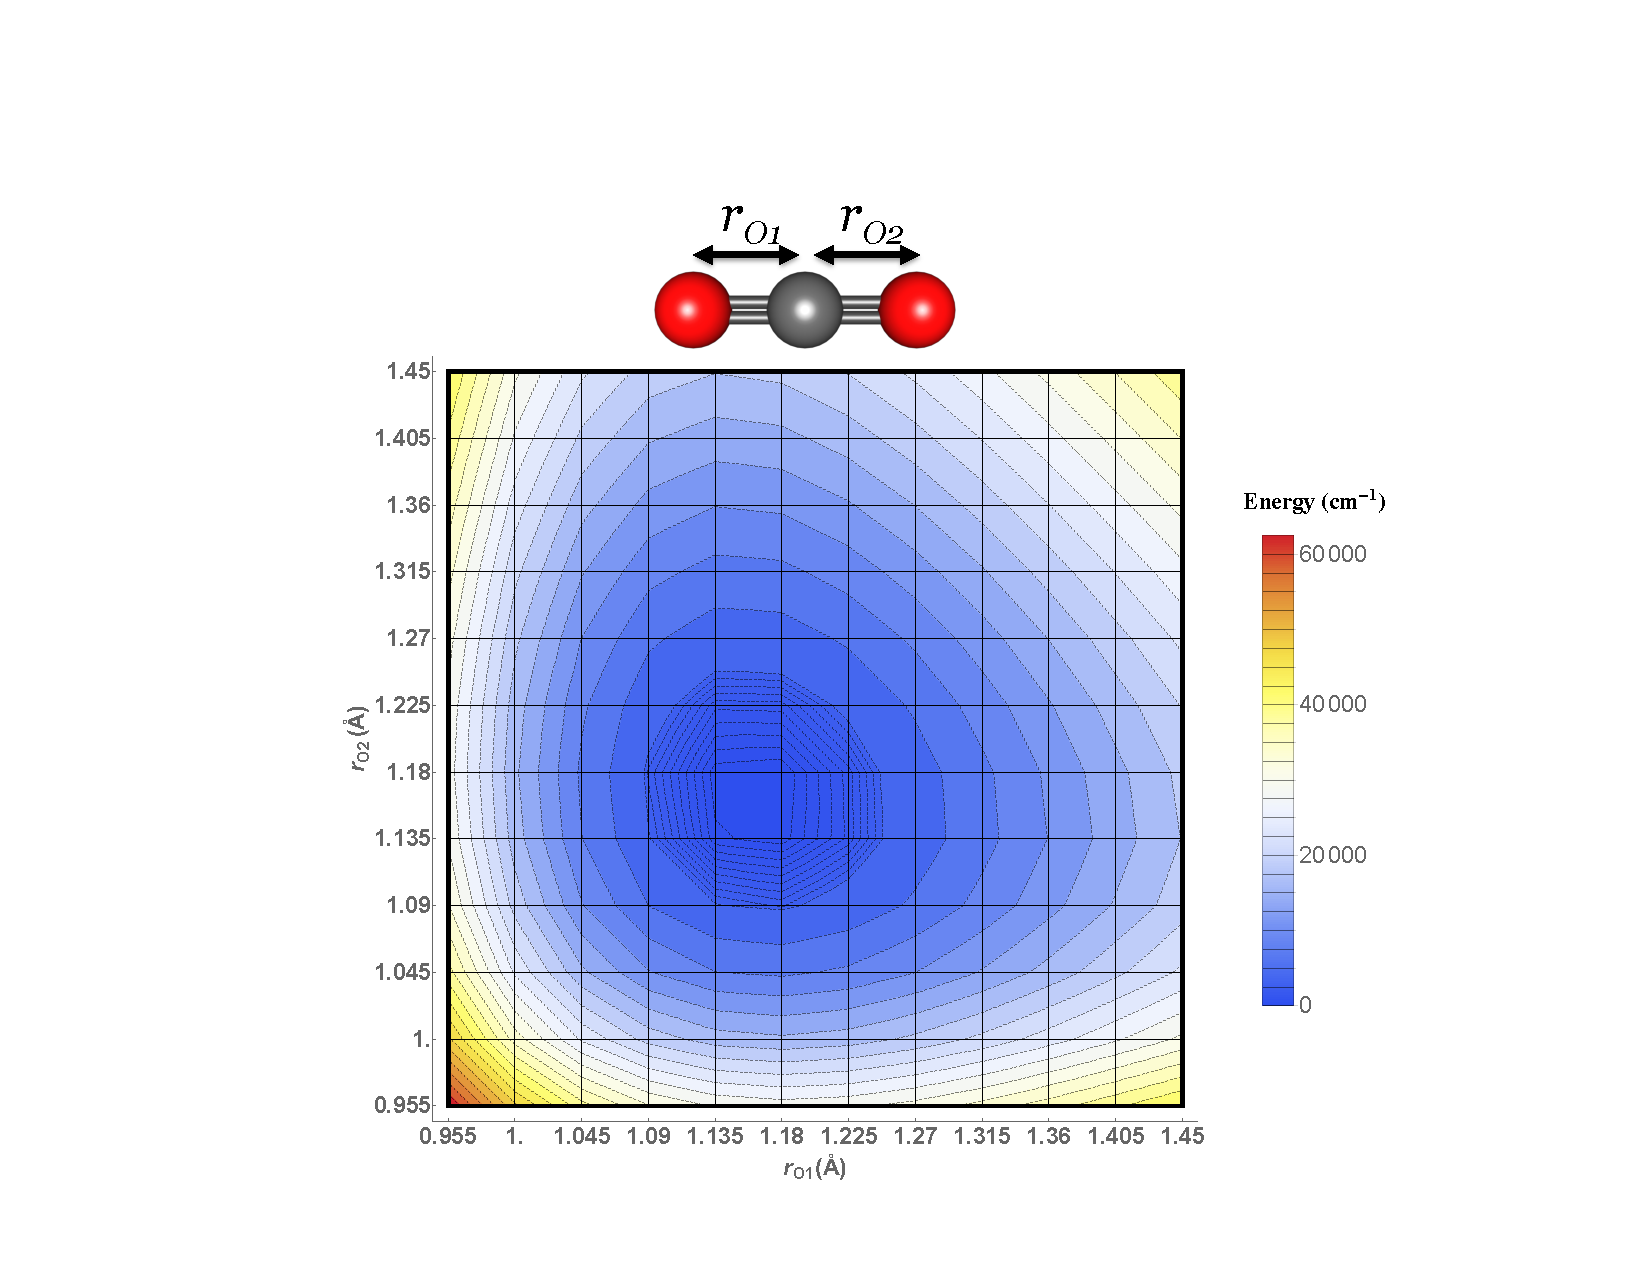
\includegraphics[scale=0.75]{paper_02/Fig1.pdf}
  \caption[DVR contour plot]{Contour plot of a discrete variable representation (DVR) of the Born\textendash{}Oppenheimer potential energy surface of gas phase \ce{CO2}. Density functional theory single point energy calculations with the B3LYP functional and the 6-311++G(d,p) basis set were performed on carbon dioxide, incrementing each CO bond's length in steps of \SI{0.045}{\angstrom}, from \SIrange{0.955}{1.45}{\angstrom}. Below a relative energy of \SI{2500}{\wavenumber}, contour lines are spaced by \SI{100}{\wavenumber}, above they are spaced by \SI{2500}{\wavenumber}. Mesh intersections indicate individual single point energy calculations. In order to calculate vibrational frequencies, this potential energy surface is incorporated into a discretized version of the Hamiltonian for the stretching modes of \ce{CO2} (Eq.~\ref{paper_02:eq:1}), which is then numerically diagonalized. The asymmetric stretch frequency is obtained from the differences between the energy levels (Eq.~\ref{paper_02:eq:2}).}
  \label{paper_02:fig:1}
\end{figure}

\section{\texorpdfstring{\caps{Sensitivity of the Calculated Vibrational Signatures to the Underlying Computational and Chemical Model}}{Sensitivity of the Calculated Vibrational Signatures to the Underlying Computational and Chemical Model}}
\label{paper_02:sec:III}

In a previous publication\cite{Brinzer2015} we identified the predominant role of CT for the asymmetric stretch frequency of \ce{CO2} in different ionic liquids. Here we aim to analyze whether our previous findings also hold when more sophisticated computational and chemical models are used. To this end, we investigate the impact of method, basis set, anharmonicity, electrostatics of the surrounding condensed phase, and solvent disorder on absolute and relative trends in the \ce{CO2} asymmetric stretch frequency.

\subsection{Method and Basis Set Dependence}
\label{paper_02:ssec:IIIA}

\begin{table}
  \centering
  \caption[Functional and basis set dependence of \texorpdfstring{\ce{CO2}}{carbon dioxide} bond lengths]{Dependence of \(r_{\ce{O}1}\) and \(r_{\ce{O}1} + r_{\ce{O}2}\) bond lengths on functional (BLYP, B3LYP, and HF) and basis set (SP, LP, VDZ, VTZ, and VQZ) for a gas-phase cluster consisting of \ce{CO2} with a cation/anion pair. All values are in \si{\angstrom}.}
  \label{paper_02:tab:1}
  \begin{tabular}{ccccccc}
    \toprule
    & \multicolumn{3}{c}{\(r_{\ce{O}1}\)} & \multicolumn{3}{c}{\(r_{\ce{O}1} + r_{\ce{O}2}\)} \\
    \midrule
    \ce{CO2} (free) & BLYP & B3LYP & HF & BLYP & B3LYP & HF \\
    SP & 1.1828 & 1.1692 & 1.1433 & 2.3656 & 2.3383 & 2.2865 \\
    LP & 1.1744 & 1.1608 & 1.1357 & 2.3487 & 2.3216 & 2.2715 \\
    VDZ & 1.1815 & 1.1674 & 1.1406 & 2.3630 & 2.3348 & 2.2811 \\
    VTZ & 1.1736 & 1.1604 & 1.1362 & 2.3472 & 2.3208 & 2.2724 \\
    VQZ & 1.1720 & 1.1588 & 1.1345 & 2.3441 & 2.3176 & 2.2690 \\
    \midrule
    & \multicolumn{3}{c}{\(r_{\ce{O}1}\)} & \multicolumn{3}{c}{\(r_{\ce{O}1} + r_{\ce{O}2}\)} \\
    \midrule
    \ce{CO2}/\ce{[BMIM][PF6]} & BLYP & B3LYP & HF & BLYP & B3LYP & HF \\
    SP & 1.1854 & 1.1723 & 1.1473 & 2.3649 & 2.3380 & 2.2871 \\
    LP & 1.1775 & 1.1646 & 1.1402 & 2.3485 & 2.3217 & 2.2725 \\
    VDZ & 1.1845 & 1.1710 & 1.1450 & 2.3622 & 2.3345 & 2.2819 \\
    VTZ & 1.1766 & 1.1639 & 1.1402 & 2.3464 & 2.3204 & 2.2727 \\
    VQZ & 1.1749 & 1.1622 & 1.1385 & 2.3434 & 2.3173 & 2.2694 \\
    \bottomrule
  \end{tabular}
\end{table}

The simplest system for examining the quantum chemical method and basis set dependence of geometries is \ce{CO2} in the gas phase. We first examine the sensitivity of the optimized geometry (Tab.~\ref{paper_02:tab:1}). Increasing the fraction of HF exchange present in a given density functional leads to a decrease in bond lengths. This bond shortening can be attributed to the lack of dynamic correlation in HF, which leads to a tendency to underestimate bond lengths. An increase in basis set size also results in decreased bond lengths, with SP bond lengths slightly longer than those calculated using VDZ, and LP bond lengths similar to those calculated using VTZ.

Bond lengths for \ce{CO2} combined with a single ion pair are shown in the lower half of Table~\ref{paper_02:tab:1}. Adding the ion pair leads to coordination of the \ce{CO2} to both the cation and anion, leading to asymmetry in the \ce{CO2} bond lengths. The effect is small, ranging from \SI{0.006}{\angstrom} at the BLYP/SP level to \SI{0.008}{\angstrom} at the HF/VDZ level. Trends in individual \ce{CO2} bond lengths with varying method and basis set agree for both ion pair-coordinated \ce{CO2} and free \ce{CO2}, even with the asymmetry. Based on these results, we estimate that the CO bond lengths presented here are converged to within \SI{0.01}{\angstrom} regarding basis set effects.

\begin{table}
  \centering
  \caption[Functional and basis set dependence of \texorpdfstring{\ce{CO2} \(\nu_3\)}{carbon dioxide asymmetric stretch} frequencies]{Dependence of \(\nu_3\) harmonic frequencies on functional (BLYP, B3LYP, and HF) and basis set (SP, LP, VDZ, VTZ, and VQZ) for an optimized gas-phase cluster consisting of \ce{CO2} and one cation/anion pair. All frequencies reported in \si{\wavenumber}. Reported frequencies are unscaled.}
  \label{paper_02:tab:2}
  \begin{tabular}{cccc}
    \toprule
    & \multicolumn{3}{c}{Method} \\
    Basis & BLYP & B3LYP & HF \\
    \midrule
    SP & 2348.88 & 2437.23 & 2582.87 \\
    LP & 2329.31 & 2419.80 & 2571.33 \\
    VDZ & 2332.11 & 2422.71 & 2577.29 \\
    VTZ & 2330.23 & 2417.28 & 2562.28 \\
    VQZ & 2322.26 & 2409.34 & 2553.85 \\
    \bottomrule
  \end{tabular}
\end{table}

Next we investigate the impact of method and basis set on the harmonic vibrational frequencies for the \(\nu_{3}\) mode in a \cotil complex (Tab.~\ref{paper_02:tab:2}). As expected, the absolute values of harmonic frequencies depend significantly on the method, overall the frequency can vary by more than \SI{200}{\wavenumber} depending on the choice of HF exchange percentage. We find a linear and positive correlation (\(R^{2} = 0.96\)) with the fraction of HF exchange present in the method for all basis sets (\hyperref[paper_02:sec:SI]{SI}). This correlation is consistent with the tendency of HF theory to overbind. Increasing the basis set size, on the other hand, results in decreasing the harmonic \ce{CO2} \(\nu_{3}\) frequency. The convergence of frequencies with basis size is rather slow, and even from VTZ to VQZ we still observe a change by \num{8}-\SI{9}{\wavenumber}. Overall, the sensitivity of the absolute vibrational frequencies to the method and basis set choice is large compared to the accuracy required to quantitatively describe the frequency shifts for \ce{CO2} solvated in different ionic liquids, which is on the order of \SI{10}{\wavenumber}.

It is therefore imperative to investigate how sensitive the prediction of relative trends is with respect to the computational approach. To this end, we consider snapshots from MD simulations (see Ref. \citep{Daly2016} for details), which allows us to test how well different computational approaches can predict \emph{trends} in dependence of the local coordination environment around the \ce{CO2} and the bulk solvent structure. Fig.~\ref{paper_02:fig:S3} shows the \ce{CO2} \(\nu_{3}\) harmonic frequencies calculated for \num{1000} statistically uncorrelated MD snapshots (0 QM/256 MM) using various SCF-type approaches, as compared to M\o{}ller\textendash{}Plesset perturbation theory to second order (MP2) as the least expensive wave function-based method that incorporates dispersion effects.\cite{WCMS:WCMS58} The predicted harmonic frequencies in Fig.~\ref{paper_02:fig:S3} are parallel to each other for most of the frequency range, independent of method and basis set choice. These results for relative trends in vibrational frequencies are highly encouraging. Aside from a multiplicative scaling factor, any of the common quantum chemical methods investigated here can qualitatively reproduce the distribution of harmonic frequencies.

Identifying the role of different intermolecular interactions in determining the vibrational signature of solvated \ce{CO2} is an important aspect of our previous and ongoing work.\cite{Brinzer2015,Ramos-Cordoba2011,Lambrecht2011c} In our previous publication,\cite{Brinzer2015} we found that the CT contribution is decisive for discriminating between the vibrational signatures of \ce{CO2} solvated in different ionic liquids. We therefore end this section by investigating the method and basis set dependence of the CT contributions to relative shifts in the \ce{CO2} asymmetric stretch frequency due to solvation. As discussed in our previous publication,\cite{Brinzer2015} CT can enter the frequency shift at two stages: (i) during the geometry optimization (i.e., influencing the geometries sampled by the solvated \ce{CO2}), and (ii) during the frequency calculation (i.e., by modifying the curvature of the potential energy surface at the point where the frequency is calculated).

To quantify the sensitivity of both mechanisms to the computational approach, we investigated the CT contributions to the calculated frequencies for both mechanisms (Table~\ref{paper_02:tab:3}). To assess the ``geometry mechanism'' (i), we calculated the frequency shift between geometries optimized using standard ``CT on'' and ALMO/SCF-MI ``CT off'' calculations, respectively. During the frequency calculation, we used the default ``CT on'' potential energy surface.

\begin{table}
  \centering
  \caption[Charge transfer dependence of \texorpdfstring{\ce{CO2} \(\nu_3\)}{carbon dioxide asymmetric stretch} frequencies]{Dependence of CT contributions to the \(\nu_3\) frequency based on functional (BLYP, B3LYP, and HF) and basis set (SP, LP, VDZ, VTZ, and VQZ). Calculations are on an optimized gas-phase cluster of \ce{CO2} with a single cation/anion pair. All frequencies reported in \si{\wavenumber}. We distinguish two mechanisms by which CT can enter the frequency: (i) a ``geometry mechanism'' where CT determines the optimized geometry of the cluster, calculated as the difference between standard harmonic frequency results at the optimized standard (``CT on'') and ALMO (``CT off'') geometries. (ii) a ``curvature mechanism'' where CT enters by modifying the force constant at the optimized geometry, calculated as the difference between the ``CT on'' and ``CT off'' frequencies at the optimized standard (``CT on'') geometry.}
  \label{paper_02:tab:3}
  \begin{tabular}{cccc}
    (i) ``Geometry Mechanism'' & \multicolumn{3}{c}{Method} \\
    \hline
    Basis & BLYP & B3LYP & HF \\
    \hline
    SP & -3.16 & -3.50 & -3.33 \\
    LP & -2.80 & -3.38 & -3.72 \\
    VDZ & -2.46 & -3.11 & -2.93 \\
    VTZ & -1.90 & -2.35 & -1.19 \\
    VQZ & -2.44 & N/A & N/A
  \end{tabular}
  \begin{tabular}{cccc}
    (ii) ``Curvature Mechanism'' & \multicolumn{3}{c}{Method} \\
    \hline
    Basis & BLYP & B3LYP & HF \\
    \hline
    SP & -2.72 & -2.86 & -2.80 \\
    LP & -1.31 & -1.25 & -1.55 \\
    VDZ & -2.92 & -2.97 & -2.53 \\
    VTZ & -1.43 & -1.33 & -0.94 \\
    VQZ & -1.18 & N/A & N/A
  \end{tabular}
\end{table}

Our results show that the frequency shift varies by up to \SI{0.9}{\wavenumber} depending on the method and by up to \SI{1.53}{\wavenumber} depending on the basis set (Tab.~\ref{paper_02:tab:3}, top). For the ``curvature mechanism'' (ii), we calculated the shift between standard ``CT on'' and ``CT off'' frequency calculations at the same, conventionally (``CT on'') optimized geometries (Tab.~\ref{paper_02:tab:3}, bottom). Here we find variations with the method of up to \SI{0.49}{\wavenumber} and up to \SI{1.86}{\wavenumber} with the basis set. Compared to the magnitude of the total CT frequency shifts, the basis set dependence is not negligible.

This finding is not surprising, because the definition of CT used within the ALMO approach is intimately linked to the locality of the basis set. However, we note that \emph{all} methods and basis sets tested here provide qualitatively similar predictions, namely a negative frequency shift between \num{-1.19} and \SI{-3.50}{\wavenumber} for the ``geometry mechanism'' and between \num{-0.94} and \SI{-2.97}{\wavenumber} for the ``curvature mechanism''. For future work, it will be useful to consider alternative definitions of CT that are less dependent on basis set locality (see e.g. Ref.~\citep{Lao2016a}).

The relative magnitudes of the ``geometry'' versus ``curvature'' mechanism results warrant some discussion, given that we found previously that the geometry contribution dominates the differentiation between different ionic liquids. According to the present results, the impact of CT via the geometry is typically bigger than the curvature effect by \SIrange{\sim 15}{35}{\percent} (with exception of the LP results, where the geometry effect is smaller than the curvature effect), but on the other hand this means the curvature effect still makes up a signification portion of the CT frequency shift. This finding may be surprising at first, but it is important to note that our previous discussion was not about the absolute magnitude of the shifts, but about the differentiation between different ionic liquids. In fact, the current results of \num{-3.50} and \SI{-2.86}{\wavenumber} are in good agreement with those from our previous publication, \SI{-3.29}{\wavenumber} and \SI{-2.29}{\wavenumber}, respectively. While the absolute values of the CT shifts are largely caused by the impact of CT on the force constants during the frequency calculation, the modification of the geometry determines the \emph{differentiation} between different ILs.

\subsection{Anharmonicity}
\label{paper_02:ssec:IIIB}

We employed a grid-based anharmonic (DVR) method to assess the effects of anharmonicity on the \ce{CO2} \(\nu_{3}\) frequency. That is, we numerically solved for the vibrational wave function on the discretized potential energy surface spanned by two degrees of freedom for the \ce{CO2} molecule (along the \ce{OCO} axis), constraining the degrees of freedom involved in \ce{CO2} bending modes, as discussed earlier. Solving for the fully anharmonic vibrational wave function is important for connecting to experiment for the following reasons. First, an accurate comparison to experiment is only possible via anharmonic calculations because experiment probes vibrational transitions that take place on the full (anharmonic) potential energy surface. Second, harmonic frequencies change their physical interpretation as vibrational energy levels when calculated away from the minimum where they pick up contributions from non-zero forces and from higher-order derivatives. For these reasons, DVR calculations are essential for being able to calculate vibrational frequencies for different geometries (MD snapshots) that are consistent with experimental conditions sampling dynamical structures away from the equilibrium geometries. Consequently, the DVR approach is instrumental for the construction of a spectroscopic map as presented in Ref. \cite{Daly2016}, as it requires sampling various (non-equilibrium) geometries from MD simulations. In this section, we investigate the impact of anharmonicity on the frequency and geometry (i.e., position expectation values) of gas-phase \ce{CO2}.

Our goal is to separate the impact of anharmonicity from the numerical errors arising from using a discretized and reduced-dimensional (2D) potential energy surface. To this end, we performed standard harmonic calculations (using analytical derivatives on the fully-dimensional surface), harmonic calculations on the discretized reduced-dimensional grid, and DVR calculations on the same grid (Tab.~\ref{paper_02:tab:4}). All potential energy surfaces were calculated at the B3LYP/LP level. The standard (analytical) harmonic calculation yielded a vibrational frequency of \SI{2420}{\wavenumber} and an equilibrium bond length of \SI{1.161}{\angstrom}.

\begin{table}
  \centering
  \caption[PES error in \texorpdfstring{\ce{CO2} \(\nu_3\)}{carbon dioxide asymmetric stretch}]{Comparison of analytical harmonic (AH), grid-based harmonic (GH), and grid-based anharmonic (DVR) absolute \(\nu_3\) frequencies for \ce{CO2} in the gas phase (B3LYP/6-311++G(d,p) potential energy surface). Reported frequencies are unscaled.}
  \label{paper_02:tab:4}
  \begin{tabular}{lcc}
    \toprule
    & \(\nu_{3}\) (\si{\wavenumber}) & \(r_{\ce{OC}}\) (\si{\angstrom}) \\
    \midrule
    analytical harmonic (AH) & 2420 & 1.161 \\
    grid-based harmonic (GH) & 2414 & 1.159 \\
    grid-based anharmonic (DVR) & 2384 & 1.165 \\
    \bottomrule
  \end{tabular}
\end{table}

For the harmonic grid-based calculations, we fit an accurate analytical potential to the grid-based potential and calculated analytical second (harmonic) derivatives. The analytical potential used an expansion in a local mode basis and included quadratic, cubic, and quartic diagonal terms, but not quartic terms in the off-diagonal (see the \hyperref[paper_02:ssec:SI5]{Supporting Information}). This approach resulted in an excellent agreement with the discrete surface (\(R^2 = 0.9997\)) and yielded a harmonic frequency of \SI{2414}{\wavenumber} and an equilibrium \ce{CO} bond length of \SI{1.159}{\angstrom}. This data suggests that the errors due to discretization and reduction of dimensionality are on the order of \SI{6}{\wavenumber} and \SI{0.002}{\angstrom}, respectively. These results support that the grid-based approach largely captures the correct physics. In comparison, the effects of anharmonicity are much larger than the discretization errors: DVR predicts a vibrational frequency of \SI{2384}{\wavenumber} (a \SI{36}{\wavenumber} red shift) and an equilibrium bond length of \SI{1.165}{\angstrom} (a \SI{0.004}{\angstrom} bond lengthening). The red shift due to anharmonicity is significantly larger than the solvation shifts observed in our previous publication.\cite{Brinzer2015}

As another point supporting the necessity for DVR calculations, we observe that the standard deviation of the calculated harmonic vibrational frequency distribution of \SI{\sim 100}{\wavenumber} (Tab.~\ref{paper_02:tab:S1}) is about an order of magnitude larger than the experimental distribution of \SIrange{\sim 6}{10}{\wavenumber}. This large error arises from the fact that harmonic calculations pick up contaminations in the frequency that grow with the displacement from the minima. As we will show in the follow-up paper,\cite{Daly2016} the anharmonic DVR calculations result in frequency distributions that are consistent with experiment. In summary, we conclude that the inclusion of anharmonic effects is imperative for constructing a spectroscopic map that allows meaningful comparison to experiment.

Since our previous results emphasized that CT is a decisive factor for the \ce{CO2} solvation shift between different ionic liquids, it is important to investigate the significance of CT in the context of anharmonic calculations. The fact that DVR calculations are agnostic toward the level of theory used to generate the discretized potential energy surface allows us to perform DVR calculations on standard (``CT on'') and ALMO/SCF-MI (``CT off'') surfaces (Tab.~\ref{paper_02:tab:5}). Excluding CT, we obtain a frequency of \SI{2399.4}{\wavenumber} and bond lengths of \SI{1.172}{\angstrom} and \SI{1.173}{\angstrom}, respectively. The slight bond length asymmetry arises from the fact that we averaged over \num{85} snapshots taken from classical MD simulations, resulting in slightly non-symmetric solvation environments (see Ref.~\citep{Daly2016} for details). Upon turning CT on, the vibrational frequency decreases to \SI{2389.5}{\wavenumber}, whereas bond lengths remain almost unchanged at \num{1.173} and \SI{1.173}{\angstrom}, respectively. This \SI{9.9}{\wavenumber} red-shift is comparable in size to experimentally observed solvation shifts for \ce{CO2} in ionic liquids,\cite{Brinzer2015,choi_vibrational_2011} which means that the anharmonic results are consistent with our earlier conclusion that CT is important to understand the vibrational signature of solvated \ce{CO2}. We plan to quantify the \emph{relative} effects of CT when studying ILs other than \ce{[C4C1im][PF6]} in future work.

\begin{table}
  \centering
  \caption[Summary of DVR data from MD snapshots]{Summary of DVR data averaged from \num{85} MD snapshots (SP = small Pople = 6-31G(d,p), LP = large Pople = 6-311++G(d,p)) at the QM/MM level, treating \ce{CO2} plus \num{2} ion pairs quantum mechanically. Reported frequencies are unscaled.}
  \label{paper_02:tab:5}
  \begin{tabular}{ccccc}
    \toprule
    PES & \(\nu_3\) (\si{\wavenumber}) & \(r_{\ce{O}1}\) (\si{\angstrom}) & \(r_{\ce{O}2}\) (\si{\angstrom}) & \(r_{\ce{O}1} + r_{\ce{O}2}\) (\si{\angstrom}) \\
    \midrule
    B3LYP/SP, CT off & 2399.4 & 1.1724 & 1.1729 & 2.3454 \\
    B3LYP/SP, CT on & 2389.5 & 1.1728 & 1.1734 & 2.3462 \\
    B3LYP/LP, CT on & 2373.9 & 1.1645 & 1.1650 & 2.3295 \\
    \bottomrule
  \end{tabular}
\end{table}

\subsection{\texorpdfstring{Molecular Mechanism of \cotil Interactions}{Molecular Mechanism of CO2-IL Interactions}}
\label{paper_02:ssec:IIIC}

We also studied the interplay between intermolecular interaction energies and the \ce{CO2} \(\nu_{3}\) frequency in order to (1) further elucidate the molecular mechanism governing \ce{CO2} solvation in ILs and to (2) inform the selection of computational approaches used to construct the \cotil spectroscopic map.\cite{Daly2016}

\subsubsection{Role of Charge Transfer and Basis Set Superposition Error}
\label{paper_02:sssec:IIIC1}

We previously concluded\cite{Brinzer2015} that the CT term, as defined in the ALMO approach, plays an important role in determining the relative frequency shifts of \(\nu_{3}\) in different ILs, primarily by modifying the \cotil cluster optimized geometry rather than by modifying the frequency calculated at a given geometry. To quantitatively analyze this conclusion, we compared predicted frequencies calculated with and without the ALMO approach (i.e., with CT on and off, respectively), at geometries again calculated with ALMO turned off and on, respectively (Fig.~\ref{paper_02:fig:2}). At the SCF geometry (i.e., geometry optimized with CT on, Fig.~\ref{paper_02:fig:2}a), the predicted frequencies for both ALMO (CT off) and standard DFT (CT on) are linearly correlated (\(R^2 = 0.978\)). At the ALMO geometry (i.e., geometry optimized with CT off, Fig.~\ref{paper_02:fig:2}b), however, neither standard DFT nor ALMO (CT off) frequency calculations correlate with the standard frequency/geometry result (\(R^2 = 0.116\) and \num{0.011} respectively).

\begin{figure}
  \centering
  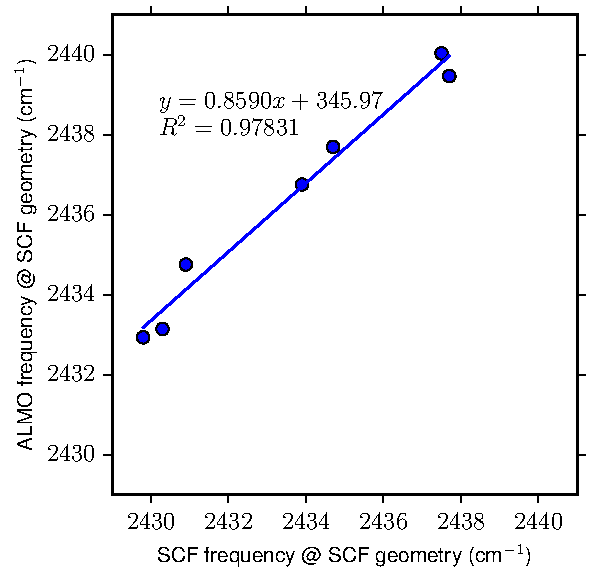
\includegraphics[scale=0.91]{paper_02/Fig2a.pdf}
  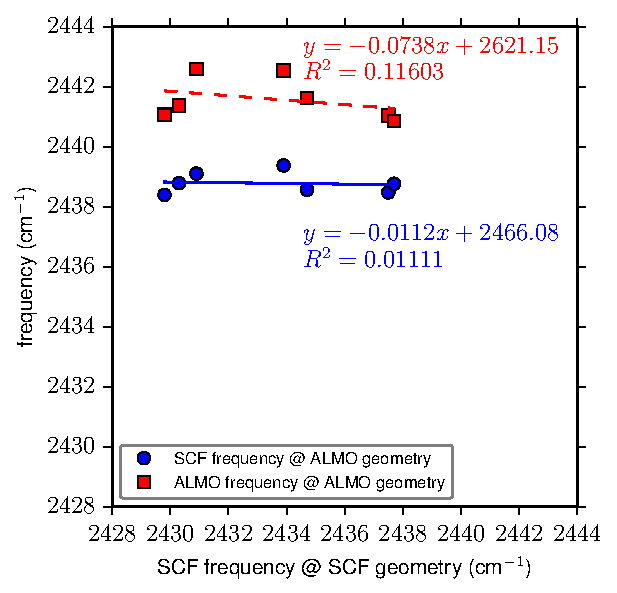
\includegraphics[scale=0.91]{paper_02/Fig2b.pdf}
  \caption[Correlation of \texorpdfstring{\ce{CO2} \(\nu_3\)}{carbon dioxide asymmetric stretch} frequencies with CT mechanisms]{Comparison of B3LYP/SP frequencies calculated (a, top) within the ALMO (CT off) approach versus standard SCF (CT on) at the standard SCF-optimized geometry and (b, bottom) at the ALMO-optimized geometry versus standard SCF-optimized geometry with Hessian within the ALMO approach (red squares) versus Hessian using standard DFT (blue triangles). The frequencies are unscaled.}
  \label{paper_02:fig:2}
\end{figure}

These findings quantitatively support our earlier conclusions that (a) CT during the frequency calculation is not significant for differentiating \(\nu_{3}\) experiencing different IL solvation environments and that (b) CT is crucial for determining the correct geometry, because removing CT during the geometry optimization eliminates this frequency differentiation.

However, ALMO simultaneously corrects for CT as well as the basis set superposition error (BSSE). We therefore performed counterpoise (CP) corrected geometry optimizations and frequency calculations to isolate artificial BSSE from physical CT effects (Fig.~\ref{paper_02:fig:3}).\cite{JCC:JCC24312,Rezac} The frequencies calculated at CP-corrected geometries and CP-\emph{un}corrected geometries correlate well (\(R^2 = 0.888\), Fig.~\ref{paper_02:fig:3}a). This finding suggests that the impact of BSSE on the geometry is small, at least as far as it is probed by the vibrational frequency. Consequently, we infer that indeed CT causes the geometry change leading to differentiation of \(\nu_{3}\) between different IL solvation environments (and not a BSSE artifact).

\begin{figure}
  \centering
  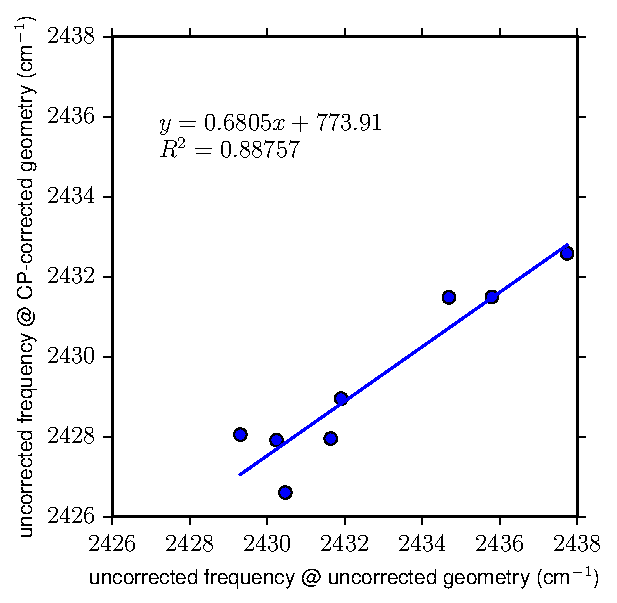
\includegraphics[scale=0.91]{paper_02/Fig3a.pdf}
  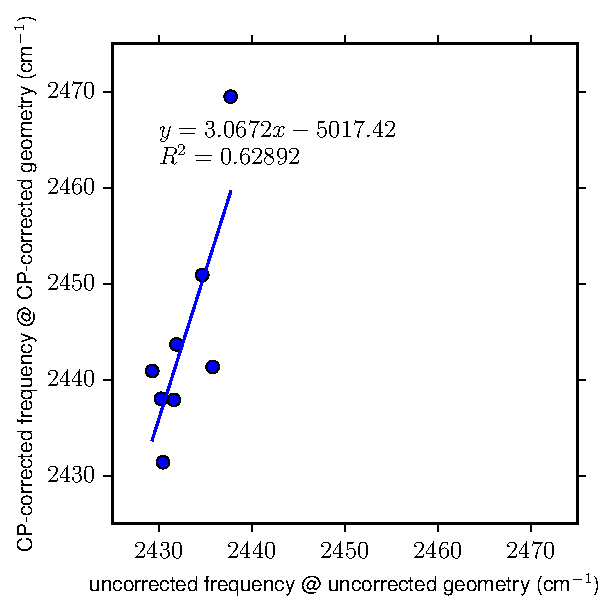
\includegraphics[scale=0.91]{paper_02/Fig3b.pdf}
  \caption[Correlation of \texorpdfstring{\ce{CO2} \(\nu_3\)}{carbon dioxide asymmetric stretch} frequencies with CP corrections]{Comparison of B3LYP/SP frequencies (a, top) calculated at counterpoise (CP) corrected geometries versus uncorrected geometries and (b, bottom) calculated using CP-corrected Hessians at CP-corrected geometries versus uncorrected Hessians at uncorrected geometries. The frequencies are unscaled.}
  \label{paper_02:fig:3}
\end{figure}

The CP-corrected frequency calculations show a somewhat smaller correlation with the CP-uncorrected frequencies (\(R^2 = 0.629\), Fig.~\ref{paper_02:fig:3}b). We believe that, for the given combination of systems and computational methodologies, the CP-\emph{un}corrected frequencies are actually more accurate than the CP-corrected frequencies for a number of reasons: (1) The trends in CP-corrected frequencies contradict our ALMO-frequency results, where ALMO predicts a \emph{negligible} impact of CT+BSSE in the frequency calculation step, whereas the CP-corrected frequency calculations suggest a significant impact of BSSE on the relative frequencies. DFT integration grid superposition errors can be excluded here because we did not find significant dependence on the grid size. (2) We suspect that the CP-correction overestimates the impact of BSSE for the given systems and computational approaches, because a detailed analysis of intermolecular interaction energies shows that, with the CP correction applied, one obtains unphysical, repulsive CT energies (see the \hyperref[SI]{SI}): ALMO-CT should always be non-repulsive, because a system would not undergo CT if it were energetically unfavorable. However, after applying a CP correction to the ALMO delocalization energy, one obtains repulsive CT energies for several MD snapshots. We conclude that the CP correction overestimates the amount of BSSE for the given system. Similar conclusions have been drawn before, for example arguing\cite{Collins1986} that the CP overcorrects for BSSE, or that BSSE is actually beneficial because it reduces basis set incompleteness.\cite{Mentel2014}

These fundamental problems in the CP-corrected frequencies manifest themselves in two findings (Tab.~\ref{paper_02:tab:S4}): (1) overestimation of the solvatochromic shifts for \(\nu_{3}\) in different ILs, and (2) incorrect ordering of the CP-corrected frequencies compared with experiment. The CP-corrected frequencies overestimate the range of solvatochromic shifts for \(\nu_{3}\) by a factor of \(5.9 \times\) when compared with experiment (\SI{38.1}{\wavenumber} versus \SI{6.5}{\wavenumber}), whereas the CP-uncorrected shifts give agree much more closely (\SI{8.4}{\wavenumber}). Furthermore, the ordering of the CP-corrected frequencies is incorrect. For example, the lowest experimental \(\nu_{3}\) frequency is found in \ce{[C4C1im][SCN]} (\SI{2336}{\wavenumber}), while the CP-corrected frequencies predict the lowest result in \ce{[C4C1im][DCA]}. The CP-uncorrected frequencies correctly predict \ce{[SCN]-} as causing the largest shift. Furthermore, anions that cause identical experimental frequencies (\ce{[Tf2N]-} and \ce{[BF4]-}: \SI{2341.7}{\wavenumber}) differ by \SI{9.6}{\wavenumber} in the CP-corrected prediction (and only by \SI{1.1}{\wavenumber} in the uncorrected calculation).

\subsection{\texorpdfstring{Energetics of \cotil Interactions and Dependence on Decomposition Approach}{Energetics of CO2-IL Interactions and Dependence on Decomposition Approach}}
\label{paper_02:sssec:IIIC2}

To understand how the choice of decomposition method affects the predicted solute\textendash{}solvent interactions, we decomposed the \cotil interaction energies of \num{15} representative MD snapshots using both ALMO and symmetry adapted perturbation theory (SAPT) calculations (Tab.~\ref{paper_02:tab:6}). Because of computational cost, the SAPT calculations were performed within the uncorrelated monomer approximation (SAPT0). While individual terms in the ALMO and SAPT0 energies do not have direct correspondence, we combined contributions into roughly comparable terms describing (a) frozen-fragment interactions (electrostatics plus Pauli repulsion, \(E_{\text{frz}}\)), (b) polarization plus Pauli repulsion (\(E_{\text{pol}}\)), (c) charge transfer plus Pauli repulsion (\(E_{\text{CT}}\)), (d) dispersion plus Pauli repulsion (\(E_{\text{disp}}\)), and (e) the total interaction energy (\(E_{\text{int}}\)).

\begin{table}
  \centering
  \caption[Comparison of ALMO and SAPT interaction energies for MD clusters]{Comparison of ALMO- versus SAPT0-decomposed interaction energies averaged over \num{15} representative molecular dynamics snapshots. ALMO calculations were performed within the SP basis to allow comparison to results from Ref. 14. For SAPT0, we report both monomer-centered basis set (MCBS) and dimer-centered basis set (DCBS) results. Energies are reported in \si{\kcal\per\mole}.}
  \label{paper_02:tab:6}
  \begin{tabular}{lcccccc}
    & & & \multicolumn{2}{c}{SAPT0 SP} & \multicolumn{2}{c}{SAPT0 jun-cc-pVTZ} \\
    component & ALMO-DFT SP & ALMO-HF SP & MCBS & DCBS & MCBS & DCBS \\
    \(E_{\text{el}}^{(10)}\) & \textemdash{} & \textemdash{} & -5.295 & -7.018 & -6.097 & -6.154 \\
    \(E_{\text{exch}}^{(10)}\) & \textemdash{} & \textemdash{} & 2.845 & 7.611 & 7.106 & 7.622 \\
    \(\mathbf{E_{\textbf{frz}}}\) & \textbf{0.500} & \textbf{0.082} & \textbf{-2.450} & \textbf{0.593} & \textbf{1.009} & \textbf{1.468} \\
    \(E_{\text{ind}}^{(20)}\) & \textemdash{} & \textemdash{} & -1.218 & -3.636 & -2.593 & -3.916 \\
    \(E_{\text{ind-exch}}^{(20)}\) & \textemdash{} & \textemdash{} & 0.009 & 2.147 & 0.921 & 2.041 \\
    \(\delta_{\text{HF}}\) & \textemdash{} & \textemdash{} & -0.839 & -0.421 & -0.801 & -0.507 \\
    \(\mathbf{E_{\textbf{pol}}}\) & \textbf{-1.241} & \textbf{-1.303} & \textbf{-2.049} & \textbf{-1.910} & \textbf{-2.473} & \textbf{-2.382} \\
    \(\mathbf{E_{\textbf{CT}}}\) & \textbf{-1.177} & \textbf{-0.102} & \multicolumn{2}{c}{\textbf{-0.280}} & \multicolumn{2}{c}{\textbf{-0.203}} \\
    \(E_{\text{disp}}^{(20)}\) & \textemdash{} & \textemdash{} & -4.193 & -5.197 & -7.323 & -8.084 \\
    \(E_{\text{disp-exch}}^{(20)}\) & \textemdash{} & \textemdash{} & 0.058 & 0.483 & 0.393 & 0.671 \\
    \(\mathbf{E_{\textbf{disp}}}\) & \textbf{\textemdash{}} & \textbf{\textemdash{}} & \textbf{-4.135} & \textbf{-4.714} & \textbf{-6.930} & \textbf{-7.413} \\
    \(\mathbf{E_{\textbf{int}}}\) & \textbf{-1.918} & \textbf{-1.323} & \textbf{-8.634} & \textbf{-6.031} & \textbf{-8.394} & \textbf{-8.326}
  \end{tabular}
\end{table}

Our results show that \(E_{\text{frz}}\) between \ce{CO2} and the IL is, on average, repulsive. ALMO predicts repulsion between \num{+0.08} and \SI{0.50}{\kcal\per\mole}, whereas SAPT0 predicts somewhat larger repulsion between \num{0.59} and \SI{1.47}{\kcal\per\mole}. The attractive interaction of \SI{-2.45}{\kcal\per\mole} at the SAPT0/SP MCBS level is likely due to an underestimation of inter-monomer overlap effects, which would result in a smaller contribution from Pauli repulsion that is recovered at the SAPT0/SP DCBS level. The finding of an overall repulsive \(E_{\text{frz}}\) is not surprising given that \ce{CO2} is a neutral, non-polar molecule, which should have little electrostatic attraction to the surrounding ions when polarization or charge delocalization are excluded.

The polarization energies contribute, as expected, to the binding. ALMO predicts polarization energies between \num{-1.24} and \SI{-1.30}{\kcal\per\mole}, whereas SAPT0 predicts somewhat more attractive energies between \num{-1.91} and \SI{-2.47}{\kcal\per\mole}.

The largest qualitative differences between predictions from ALMO and SAPT0 are found for charge transfer and dispersion energies. The ALMO-HF CT (\SI{-0.10}{\kcal\per\mole}) is comparable in magnitude to the SAPT0 CT (\SI{-0.28}{\kcal\per\mole}), whereas the ALMO-DFT CT is significantly larger (\SI{-1.18}{\kcal\per\mole}). Overestimation of CT effects is expected for DFT-based ALMO because of self-interaction error, leading to spurious delocalization of electrons. The dispersion component does not exist in the SCF-based ALMO approach used here and can therefore not be compared.

We note, importantly, that SAPT0 predicts the dispersion contribution of \num{-4.14} to \SI{-7.41}{\kcal\per\mole} to be the major binding contribution for the \cotil interactions. In contrast, ALMO-DFT predicts polarization and CT to be the dominant and equally important contributions to the overall binding, and ALMO-HF predicts polarization to be the largest contribution. Overall, the ALMO total binding energies range from \num{-1.32} to \SI{-1.92}{\kcal\per\mole}, whereas SAPT0 binding energies within the MCBS and DCBS are \num{-6.03} and \SI{-8.63}{\kcal\per\mole}, respectively. Given the magnitude of the dispersion interaction, it is not surprising that SAPT0 predicts a much more attractive total binding energy.

The three approaches used here disagree on the dominating mechanism of binding: ALMO-HF favors polarization, ALMO-DFT polarization in combination with CT, and SAPT0 predicts dispersion as the most important binding component. Interestingly, though, individual energy contributions that exist both in ALMO and SAPT0 agree qualitatively. We expect that the SAPT0/jun-cc-pVTZ DCBS numbers are the most accurate of the results reported here because these results are free of SIE (unlike ALMO-DFT) and explicitly account for inter-monomer correlation (dispersion) effects.

The conclusion changes when comparing \emph{relative trends} in binding energies between different MD snapshots. Comparing the correlation coefficients for linear regression analysis between individual energy components and the total energies (Tab.~\ref{paper_02:tab:7}a), \emph{all} of the methods predict that the frozen monomer electrostatics plus Pauli repulsion component (\(E_{\text{frz}}\)) is the single most important contribution to trends in the total energy (\(R^2 = \numrange[range-phrase = --]{0.870}{0.944}\)). This finding implies that, although ALMO and SAPT0 disagree on the identity of the largest absolute energy component, they agree that the \(E_{\text{frz}}\) is most important to capture differential effects between different MD snapshots. This finding is somewhat surprising, given that \(E_{\text{frz}}\) is a rather small energy contribution on an absolute scale, whereas dispersion makes up the largest contribution to the total binding energy. However, this trend shows that dispersion varies less than the frozen-fragment interaction across different points on the potential energy surface.

\begin{table}
  \centering
  \caption[Correlation between ALMO and SAPT terms]{Correlation coefficients (\(R^2\)) between different solute-solvent interaction energy components as calculated at the ALMO-DFT (B3LYP), ALMO-HF, and SAPT0 level within the SP basis. (a) Comparison between individual components and the total interaction energy (\(E_{\text{tot}}\)) calculated for each methodology. (b) Correlation coefficients between contributions to the \cotil interaction energy calculated via ALMO as compared to the corresponding SAPT0 energy terms. Reported SAPT0 results are within the dimer-centered basis set (DCBS), except for the charge transfer component, which is calculated as the difference between monomer- and dimer-centered basis set results for the induction energy.}
  \label{paper_02:tab:7}

  (a)

  \begin{tabular}{lccc}
    \toprule
    Component & ALMO-DFT & ALMO-HF & SAPT0 \\
    \midrule
    \(E_{\text{frz}}\) & 0.887 & 0.944 & 0.870 (\(E_{\text{el}}\): 0.602, \(E_{\text{exch}}\): 0.073) \\
    \(E_{\text{pol}}\) & 0.170 & 0.087 & 0.073 \\
    \(E_{\text{CT}}\) & 0.225 & 0.270 & 0.093 \\
    \(E_{\text{disp}}\) & \textemdash{} & \textemdash{} & 0.150 \\
    \bottomrule
  \end{tabular}

  (b)

  \begin{tabular}{lcc}
    \toprule
    Component (ALMO \textemdash{} SAPT0) & ALMO-DFT & ALMO-HF \\
    \midrule
    \(E_{\text{frz}}\) \textemdash{} \(E_{\text{el}} + E_{\text{exch}}\) & 0.989 & 0.993 \\
    \(E_{\text{pol}}\) \textemdash{} \(E_{\text{ind}} + E_{\text{ind-exch}} + \delta_{\text{HF}}\) & 0.887 & 0.927 \\
    \(E_{\text{CT}}\) \textemdash{} \(E_{\text{CT}}\) & 0.720 & 0.383 \\
    \(E_{\text{tot}}\) \textemdash{} \(E_{\text{tot}}\) & 0.913 & 0.927 \\
    \bottomrule
  \end{tabular}
\end{table}

These findings have at least two important implications. Since ALMO-DFT, ALMO-HF and SAPT0 qualitatively agreed on the \(E_{\text{frz}}\) component, all of these methods should correctly describe relative trends in the energetics across different MD snapshots. That is, despite self-interaction error and the lack of dispersion interactions, DFT is expected to correctly capture energetic trends across different snapshots along the potential energy surface. Furthermore, any spectroscopic map (\emph{i.e.} a map between \ce{CO2} geometry and vibrational frequency) \emph{must} contain an electrostatic term to capture these leading-order relative effects. ALMO and SAPT approaches predict the CT and dispersion terms to be the second most important for relative frequency trends, respectively (\(R^2 = 0.225 -- 0.270\) for ALMO-CT and \(R^2 = 0.150\) for SAPT-dispersion), which are expected to show a different geometry dependence. Consequently, adding a Lennard-Jones type potential to the spectroscopic map may allow implicit collection of these non-electrostatic terms.

The good correlation between ALMO and SAPT0 electrostatic plus Pauli repulsion terms is also demonstrated by a term-by-term comparison (Tab.~\ref{paper_02:tab:7}b): ALMO-DFT has a correlation coefficient of \num{0.989} with SAPT0, and ALMO-HF has one of \num{0.993}. Polarization energies also correlate well (\(R^2 = 0.887\) and \num{0.927}, respectively). The lowest agreement is found for the charge transfer term (\(R^2 = 0.720\) and \num{0.383}, respectively). This low degree of correlation is somewhat surprising, since the formal definitions of charge transfer are very similar between ALMO and SAPT0 \textemdash{} both involve the difference between energetics calculated for a monomer-centered and a dimer-centered basis set. Furthermore, the absolute magnitude of the ALMO-HF CT term agrees better with SAPT0, but it shows less correlation across different MD snapshots. The ALMO-DFT CT term, on the other hand, is much larger than in SAPT0, but seems to correlate better with trends across MD snapshots, although one would expect the ALMO-DFT results to be less reliable due to self-interaction error. This large difference between ALMO-DFT and SAPT0 CT energies remains even with the use of range-separated density functionals, but we note that adding a dispersion correction leads to a good agreement between DFT-D and SAPT0 (Table~\ref{paper_02:tab:S3}).

Interestingly, the ALMO total binding energies correlate well with SAPT0 binding energies (\(R^2 = 0.913\) and \num{0.927}, respectively), even though ALMO binding energies are generally much smaller than SAPT0 energies. This good correlation can be understood by considering that the major discrepancy between ALMO and SAPT0 binding energies comes from the dispersion term, which, despite its large magnitude, is relatively constant across MD snapshots and therefore does not correlate strongly with the total binding energy.

In summary, despite shortcomings in capturing the nuanced physics of intermolecular \cotil binding, DFT- and even HF-based approaches are expected to produce qualitatively correct trends, if the goal is to compare binding energies across different MD snapshots.  Consequently, we expect that DFT will capture qualitative trends in the potential energy landscape, and can be safely used to generate DVR potential energy surfaces for DVR used to construct and validate a spectroscopic map for \ce{CO2} in ionic liquids.

\subsection{Electrostatic Interactions with the Extended Solvent Phase}
\label{paper_02:ssec:IIID}

Our previous publication\cite{Brinzer2015} used a rather crude gas-phase cluster model for the solvated \ce{CO2}. Here we investigate the effect of adding a more extended solvation environment by varying the MM region (Fig.~\ref{paper_02:fig:4}). Calculations were performed at the B3LYP/SP level of theory, with the ionic liquid molecules represented as point charges. Each data point is an average from \num{25} snapshots, which were selected using the sampling scheme previously described.

\begin{figure}
  \centering
  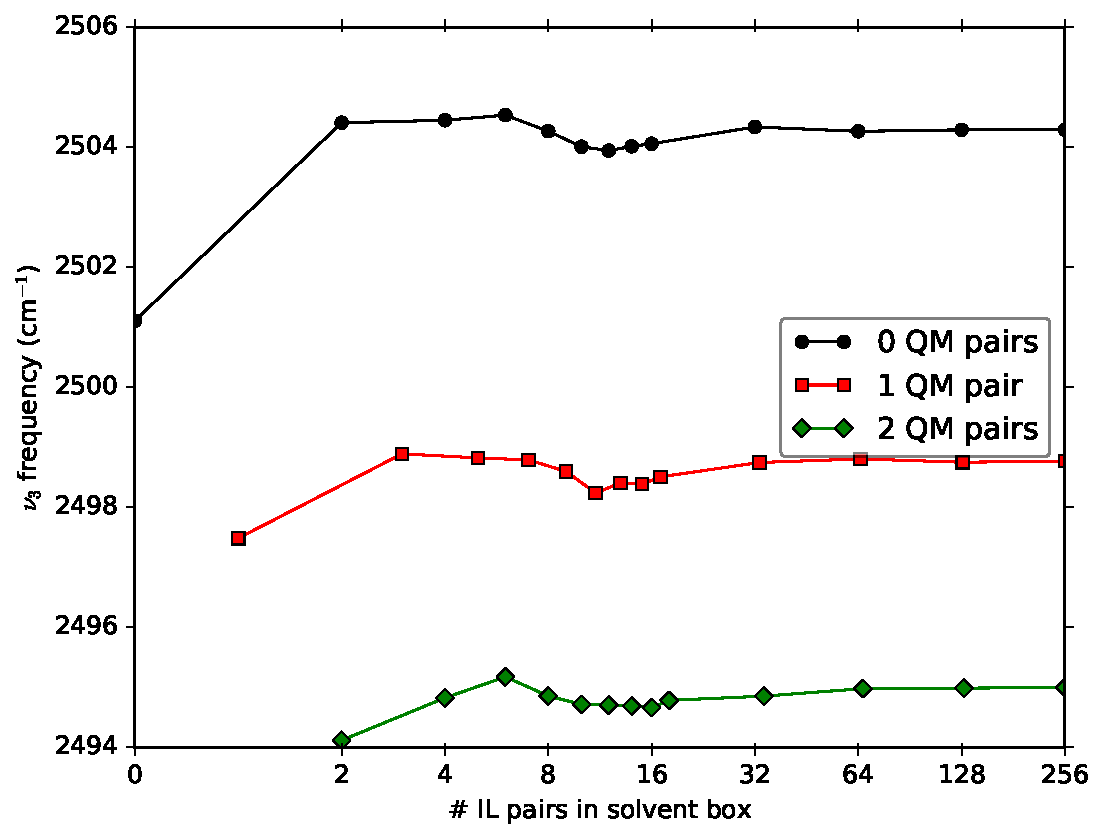
\includegraphics[width=\textwidth]{paper_02/frequency_same_set_2QM_convergence.pdf}
  \caption[Effect of QM and MM region size on \texorpdfstring{\ce{CO2} \(\nu_3\)}{carbon dioxide asymmetric stretch} QM/MM frequencies]{Dependence of harmonic \(\nu_3\) frequencies (unscaled) on the solvent box size (B3LYP/SP potential energy surface).}
  \label{paper_02:fig:4}
\end{figure}

As expected, the largest frequency shifts occur when the first few solvent ion pairs are added to the solvated \ce{CO2}. The frequency is converged to within \SI{1}{\wavenumber} at a solvent layer size of \num{\sim 32} ion pairs, which corresponds to a solvent droplet of radius \SI{\sim 14}{\angstrom}. This relatively fast convergence (from the perspective that the solvent molecules are charged) is attributed to electrostatic screening due to the solvent.

We observe qualitatively the same trends and convergence patterns independent of whether a pure point charge embedding is used or whether one or two ion pairs are included at the QM level. This finding indicates that solvation boxes including \num{\sim 32} or more ion pairs are sufficient to converge electrostatic effects on the vibrational frequency independent of how many solvent molecules are treated at the QM level. However, we notice that there is a significant shift in frequencies depending on the size of the QM region. The fact that increasing the solvent box (treated as classical point charges) does not cause the differently sized QM regions to reconcile indicates that the underlying effects are quantum mechanical (as opposed to purely electrostatic) in nature. It is therefore indicated to further investigate the dependence of the frequency on the size of the QM region.

\subsection{Quantum Mechanical Interactions with the Solvation Shell}
\label{paper_02:ssec:IIIE}

To test for convergence of the asymmetric frequency with respect to the size of the QM region, we selected a subset of \num{10} snapshots from the MD trajectories and carried out QM/MM harmonic frequency calculations with increasing numbers of anion\textendash{}cation pairs treated quantum mechanically (Fig.~\ref{paper_02:fig:5}). These snapshots were carefully selected to sample the entire range of local vibrational frequencies encountered in the MD trajectories and were averaged by weighting with the appropriate probabilities for each frequency bin. We therefore expect the following results to be representative of large parts of the entire potential energy surface sampled. We tested several functions to fit the mean frequency \(\overline{\nu}\) (i.e., the weighted average over all sampled frequencies) versus the QM region size, and found that an exponential decay function yields the best overall fit,
\begin{equation*}
  \overline{\nu}\left( n \right) = a\exp{\left( -kn \right)} + c
\end{equation*}
where \(n\) is the size of the QM region (measured in number of ion pairs) and \(a, k\), and \(c\) are constants. The quality of the resulting fit was excellent (\(R^2 = 0.99\)), which allowed us to extrapolate the average frequency to infinite QM region size with high confidence. This extrapolated frequency then allows us to assess the accuracy (convergence) of QM/MM calculations with differently sized QM regions.

\begin{figure}
  \centering
  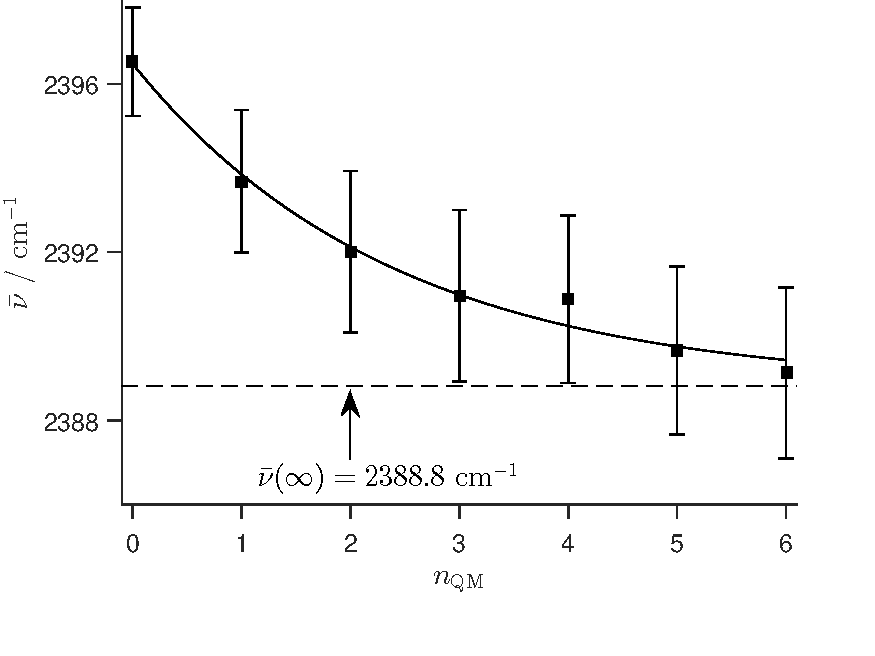
\includegraphics{paper_02/Fig5.pdf}
  \caption[DVR convergence with respect to number of QM ion pairs]{Dependence of DVR \(\nu_{3}\) mean frequency (\(\overline{\nu}\)) on the number of solvent ion pairs treated quantum mechanically (\(n_{QM}\)). Mean frequencies were calculated from \(N = 10\) representative MD snapshots using a B3LYP/SP potential energy surface. Error bars represent the standard deviation of the mean (\(SD_{\overline{x}} = \sigma_{x}/\sqrt{N}\)). The data were fitted to an exponential decay (\({\overline{\nu}}_{QM} = A\exp\left( - kn_{QM} \right) + {\overline{\nu}}_{converged}\)), with weights of \(1/SD_{\overline{x}}^{2}\) (\(R^2 = 0.99\)). The resulting estimate for the fully converged frequency at this level of theory is \(2388.8 \pm \SI{1.5}{\wavenumber}\).}
  \label{paper_02:fig:5}
\end{figure}

We determine the converged frequency to be \(c = 2388.8 \pm \SI{1.5}{\wavenumber}\) (Fig.~\ref{paper_02:fig:5}). This data indicates that the \num{6} QM calculations are nearly numerically converged (\(\overline{\nu}\left( 6 \right) - \overline{\nu}\left( \infty \right) = \SI{0.3}{\wavenumber}\)). To test the qualitative accuracy of the calculations using smaller QM regions, we examined the correlation between frequencies calculated with \(n = 0-5\) QM pairs and \num{6} QM pairs for each snapshot (for details, see Supporting Information). We find that the \(n = 0-1\) results do not correlate well with the \(n = 6\) benchmark (\(R^{2} = 0.41\) and \num{0.66}, respectively). The \(n = 2\) calculations yield an acceptable correlation coefficient of \(R^2 = 0.82\) at a \num{\sim 9}-fold reduced computational cost compared to \(n = 6\) (\num{\sim 0.8} versus \num{\sim 7} CPU hours for a single point calculation). The \(n = 3-4\) calculations show even better correlations with \(R^2 = 0.87 -- 0.96\), respectively, but the computational cost increase to \num{\sim 3} CPU hours does not appear justified. In summary, the \(n = 2\) calculations reproduce trends in the \ce{CO2} asymmetric stretch frequency reasonably well and offer a good balance between accuracy and cost for our DVR calculations.

\subsection{Predicted Solvation Shift}
\label{paper_02:ssec:IIIF}

A central objective of this publication is to establish a computational approach that will allow us to develop a reliable spectroscopic map for the prediction and interpretation of 2D-IR spectroscopic signatures for \ce{CO2} solvated in ionic liquids. While the spectroscopic map and its validation are the subject of the second publication in this series, we can use the predicted solvation shift (i.e., the frequency shift between gas-phase \ce{CO2} and dissolved in \ce{[C4C1im][PF6]}) as a first indicator for the quality of the computational and chemical model. We note that absolute frequencies are very hard to reproduce with all but the most sophisticated quantum chemical approaches, which are prohibitively expensive for the present application. We therefore scale the calculated frequencies by a factor of \num{0.9855} so the DVR/B3LYP/LP gas-phase result of \SI{2384}{\wavenumber} (Tab.~\ref{paper_02:tab:4}) agrees with the experiment (\SI{2349}{\wavenumber}). At the proposed DVR/B3LYP/LP level (within a QM/MM approach with \(n = 2\) ion pairs in the QM region and sampling from \num{85} MD snapshots for the solvated \ce{CO2}), the scaled frequency of the solvated \ce{CO2} is \SI{2339}{\wavenumber} (Tab.~\ref{paper_02:tab:5}). The predicted solvation frequency shift is then \SI{-10}{\wavenumber}, which is in good agreement with the experimental solvation shift of \SI{-6.8}{\wavenumber}. We note that these results were calculated from only \num{85} MD snapshots and are therefore probably not statistically converged. We will present an in-depth validation of convergence with respect to number of MD steps in the subsequent paper. The already rather nice agreement makes us optimistic that an accurate spectroscopic map can be developed using the computational approach proposed here.

\section{\texorpdfstring{\caps{Conclusions}}{Conclusions}}
\label{paper_02:sec:IV}

This work provides fundamental insights into the molecular origins of the vibrational frequency shifts of \ce{CO2} in ionic liquids. First, we validated the computational methodology used for predicting vibrational frequencies \textemdash{} as defined by basis set, wave function or density functional method, size of the QM region, and the role of anharmonicity. Second, we analyzed the physical origins of \cotil binding and its interplay with the vibrational frequency shifts using ALMO and SAPT energy decomposition schemes. Our calculations provide insights that are perhaps quite surprising, but definitely nuanced. In a previous publication we concluded that, unlike for other vibrational chromophores, electrostatics alone poorly predict the vibrational frequency shifts for \ce{CO2} in different ILs. From ALMO-EDA we concluded that this frequency shift between different ionic liquids is actually not driven by the electrostatics, but by charge transfer from the anion. This work confirms that our previous results are qualitatively independent from the choices of basis set, ab initio method, and treatment of anharmonicity, confirming the validity of our previous results within the ALMO framework. For different points on the potential energy surface of a \emph{single} ionic liquid (here: \ce{[C4C1im][PF6]}), however, the energetics are dominated by electrostatics plus Pauli repulsion. This frequency shift mechanism is surprising, firstly because it is fundamentally different from the mechanism that drives the \ce{CO2} frequency shift between different ILs, and secondly because electrostatics plus Pauli repulsion is a relatively small energetic contribution compared to, e.g., dispersion interactions, which one would therefore expect to dominate the frequency shifts. An important practical consequence of this finding is that density functional theory is expected to be sufficiently accurate for constructing potential energy surfaces for \ce{CO2} in \ce{[C4C1im][PF6]}, as needed for the DVR calculations to construct a reliable spectroscopic map.

Similarly, we established appropriate computational and chemical models for treating the extended solvent environment. Our calculations show that a QM/MM treatment with \ce{CO2} plus \num{2} cation\textendash{}anion pairs treated quantum mechanically yields vibrational frequencies that are sufficiently close to the converged QM results. Furthermore, adding around \num{32} ion pairs to the MM solvent box leads to vibrational frequencies converged to within \SI{1}{\wavenumber}.

In summary, this work elucidated the molecular binding mechanism of \ce{CO2} in the \ce{[C4C1im][PF6]} ionic liquid and its interplay with the \ce{CO2} asymmetric stretch frequency \(\nu_{3}\), and established computational protocols for the reliable construction of spectroscopic maps for simulating ultrafast 2D-IR data of \ce{CO2} solvated in ILs. For future publications, it will be interesting to employ similar energy decomposition schemes to analyze the energetics and spectral signatures of other chromophores such as \ce{SCN-}, \ce{N3-}, amides, and phosphates.

\section{\texorpdfstring{\caps{Acknowledgements}}{Acknowledgements}}

SAC is grateful for financial support from the National Science Foundation (CHE-1565471), the American Chemical Society Petroleum Research Fund (52648-ND6), and the Sustainable Energy Initiative at the University of Notre Dame. This material is based upon work supported by the National Science Foundation under Grant No. (CHE-1454105). TAB acknowledges support of the Pittsburgh Quantum Institute. DSL thanks the University of Pittsburgh for start-up funding. EJB thanks Dr. Mary Sherman for performing initial SAPT calculations and cclib\cite{OBoyle2008,Berquist2015} for the analysis framework. The authors thank Prof. Kenneth D. Jordan for helpful discussions. SAC and CAD are also thankful for high-performance computing resources and support from the Center for Research Computing at the University of Notre Dame.~EJB and DSL thank the Center for Simulation and Modeling at the University of Pittsburgh for providing computational resources.

\section{\texorpdfstring{\caps{Supporting Information}}{Supporting Information}}
\label{paper_02:sec:SI}

Statistics on calculated harmonic frequencies across different MD snapshots, bin sizes and weights for 15-25 representative structures sampled from MD snapshots, method and basis set dependence, QM/MM box size convergence, quartic fit of the DVR potential energy surface, and effects of BSSE and CP on harmonic frequencies of \ce{CO2} asymmetric stretch across different ionic liquids.

\begin{landscape}
  \begin{table}
    \centering
    \caption[Statistical distribution of harmonic frequencies for MD snapshots]{Statistics for dependence of \ce{CO2} asymmetric stretch frequencies on quantum chemical method and basis set dependence on \num{1000} MD snapshots, 0 QM/256 MM. All frequencies in \si{\wavenumber}.}
    \label{paper_02:tab:S1}
    \begin{tabular}{ccccccccc}
      \toprule
      method & basis set & min & max & range & mean & median & standard deviation (population) & standard deviation (sample) \\
      \midrule
      BLYP & 6-31G(d,p) & 2179.26 & 2915.23 & 735.97 & 2551.84 & 2552.16 & 112.92 & 112.86 \\
      TPSS & 6-31G(d,p) & 2247.16 & 2967.72 & 720.56 & 2611.68 & 2612.06 & 110.39 & 110.33 \\
      B3LYP & 6-31G(d,p) & 2141.31 & 2892.22 & 750.91 & 2522.55 & 2522.96 & 115.09 & 115.03 \\
      \(\omega\)B97X-D & 6-31G(d,p) & 2138.86 & 2894.15 & 755.29 & 2523.38 & 2523.93 & 114.14 & 114.08 \\
      HF & 6-31G(d,p) & 1990.89 & 2814.31 & 823.42 & 2415.50 & 2416.41 & 125.46 & 125.40 \\
      RI-MP2 & 6-31G(d,p) & 2264.73 & 2964.82 & 700.09 & 2615.07 & 2615.27 & 107.68 & 107.62 \\
      BLYP & cc-pVTZ & 2083.99 & 2802.55 & 718.56 & 2448.66 & 2449.17 & 110.15 & 110.10 \\
      TPSS & cc-pVTZ & 2164.75 & 2871.70 & 706.95 & 2523.22 & 2523.74 & 108.27 & 108.22 \\
      B3LYP & cc-pVTZ & 2047.30 & 2781.22 & 733.92 & 2420.89 & 2421.51 & 112.37 & 112.31 \\
      \(\omega\)B97X-D & cc-pVTZ & 2048.35 & 2787.24 & 738.89 & 2425.06 & 2425.52 & 111.67 & 111.61 \\
      HF & cc-pVTZ & 1908.93 & 2714.98 & 806.05 & 2325.54 & 2326.49 & 122.60 & 122.54 \\
      RI-MP2 & cc-pVTZ & 2165.68 & 2842.63 & 676.95 & 2504.51 & 2504.63 & 104.39 & 104.34 \\
      \bottomrule
    \end{tabular}
  \end{table}
\end{landscape}

\begin{landscape}
  \begin{table}
    \centering
    \caption[Histogram and weights of frequency distributions from MD snapshots]{Weights and bin counts for each quantum chemical method and basis set, 0 QM/256 MM. Weights from B3LYP/6-31(d,p) are used for selecting the structures for box size dependence and SAPT calculations.}
    \label{paper_02:tab:S2}
    \small
    \begin{tabular}{llllll}
      \toprule
      method & basis set & bin edges & histogram & weights & sum (histogram) \\
      \midrule
      BLYP & 6-31G(d,p) & [2269.54 2382.46 2495.38 2608.30 2721.23 2834.13] & [59 245 398 224 64] & [0.05959596 0.24747475 0.40202020 0.22626263 0.06464646] & 990 \\
      TPSS & 6-31G(d,p) & [2335.71 2446.10 2556.49 2666.88 2777.27 2887.66] & [59 244 400 223 64] & [0.05959596 0.24646465 0.40404040 0.22525253 0.06464646] & 990 \\
      B3LYP & 6-31G(d,p) & [2234.82 2349.91 2465.00 2580.09 2695.18 2810.27] & [59 245 398 224 64] & [0.05959596 0.24747475 0.40202020 0.22626263 0.06464646] & 990 \\
      \(\omega\)B97X-D & 6-31G(d,p) & [2238.04 2352.18 2466.31 2580.45 2694.59 2808.72] & [57 241 401 225 63] & [0.05775076 0.24417427 0.40628166 0.22796353 0.06382979] & 987 \\
      HF & 6-31G(d,p) & [2101.85 2227.31 2352.77 2478.23 2603.69 2729.15] & [61 240 399 228 63] & [0.06155399 0.24217962 0.40262361 0.23007064 0.06357215] & 991 \\
      RI-MP2 & 6-31G(d,p) & [2345.88 2453.56 2561.23 2668.91 2776.58 2884.26] & [59 246 398 223 64] & [0.05959596 0.24848485 0.40202020 0.22525253 0.06464646] & 990 \\
      BLYP & cc-pVTZ & [2173.29 2283.44 2393.59 2503.74 2613.89 2724.04] & [59 245 398 224 64] & [0.05959596 0.24747475 0.40202020 0.22626263 0.06464646] & 990 \\
      TPSS & cc-pVTZ & [2252.54 2360.81 2469.09 2577.36 2685.64 2793.91] & [59 245 396 226 64] & [0.05959596 0.24747475 0.40000000 0.22828283 0.06464646] & 990 \\
      B3LYP & cc-pVTZ & [2139.97 2252.34 2364.70 2477.07 2589.44 2701.80] & [59 244 399 224 64] & [0.05959596 0.24646465 0.40303030 0.22626263 0.06464646] & 990 \\
      \(\omega\)B97X-D & cc-pVTZ & [2145.89 2257.56 2369.22 2480.89 2592.56 2704.22] & [57 243 399 225 63] & [0.05775076 0.24620061 0.40425532 0.22796353 0.06382979] & 987 \\
      HF & cc-pVTZ & [2019.04 2141.64 2264.24 2386.84 2509.44 2632.04] & [61 240 401 226 63] & [0.06155399 0.24217962 0.40464178 0.22805247 0.06357215] & 991 \\
      RI-MP2 & cc-pVTZ & [2243.53 2347.92 2452.32 2556.71 2661.11 2765.50] & [59 247 394 226 64] & [0.05959596 0.24949495 0.39797980 0.22828283 0.06464646] & 990 \\
      \bottomrule
    \end{tabular}
  \end{table}
\end{landscape}

\subsection{Method and Basis Set Dependence of Harmonic Frequencies}
\label{paper_02:ssec:SI3}

It is imperative to investigate how sensitive the prediction of relative trends is with respect to the computational approach. To this end, we consider snapshots from MD simulations (see Ref. \citep{Daly2016} for details), which allow us to test how well different computational approaches can predict \emph{trends} in dependence of the local coordination environment around the \ce{CO2} and the bulk solvent structure. Fig.~\ref{paper_02:fig:S3} shows the \ce{CO2} \(\nu_{3}\) harmonic frequencies calculated for \num{1000} statistically uncorrelated MD snapshots (0 QM/256 MM) using various SCF-type approaches, as compared to Møller-Plesset perturbation theory to second order (MP2) as the least expensive wave function-based method that incorporates dispersion effects.\cite{WCMS:WCMS58} The predicted harmonic frequencies in Fig.~\ref{paper_02:fig:S3} are parallel to each other for most of the frequency range, independent of method and basis set choice. In fact, there is almost complete overlap between the B3LYP/SP and \(\omega\)B97X-D/SP distributions, and to a lesser degree for B3LYP/VTZ and \(\omega\)B97X-D/VTZ. There is minor crossing of curves in two instances, 1. TPSS/VTZ with \(\omega\)B97X-D/SP, and 2. HF/SP with both B3LYP/VTZ and \(\omega\)B97X-D/VTZ, but nevertheless the conservation of qualitative trends seems excellent. The ordering of calculated frequencies is, from smallest to largest, HF, B3LYP, \(\omega\)B97X-D, BLYP, TPSS, and MP2, using the SP basis set. Within the VTZ basis, the ordering of MP2 and TPSS is interchanged. As expected, the MP2 results are most sensitive to the basis set size, as wave-function based correlation methods require larger basis sets for convergence compared to self-consistent field approaches (HF and DFT). The VTZ basis set predicts frequency distributions that are red-shifted compared to the SP basis set, in agreement with the trends observed from Table~\ref{paper_02:tab:2}.

These results for relative trends in vibrational frequencies are highly encouraging. Aside from a multiplicative scaling factor, any of the common quantum chemical methods investigated here can qualitatively reproduce the distribution of harmonic frequencies. The similarity in performance between B3LYP and \(\omega\)B97X-D is somewhat surprising, as the former is a global hybrid with a fixed fraction of HF exchange over all interelectronic distances, and \(\omega\)B97X-D is a range-separated functional with a variable fraction of HF exchange. An explanation of this observation will be provided together with the SAPT results.

\begin{figure}
  \centering
  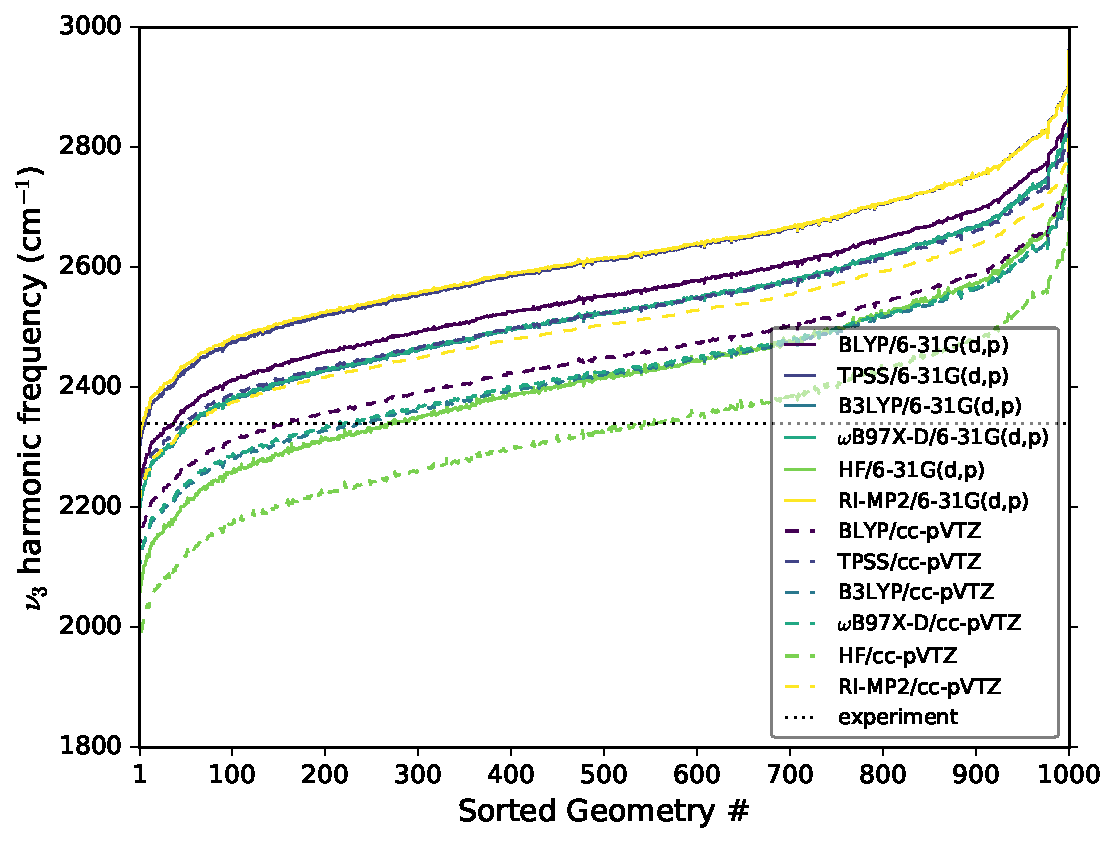
\includegraphics[width=\textwidth]{./paper_02/snapshots_ordered_0QM_256MM.pdf}
  \caption[Spread of method and basis set dependence of MD snapshots]{Harmonic \(\nu_{3}\) frequencies (unscaled) for different methods and basis sets, ordered from lowest to highest frequency according to MP2/VTZ (0 QM/256 MM). The TPSS meta-GGA\cite{Tao2003} and the \(\omega\)B97X-D\cite{Chai2008} hybrid GGA density functionals are included as representatives of more recent functionals. \(\omega\)B97X-D is both a range-separated functional, with a minimum 22\% HF exchange at \(r_{e} = 0\), increasing smoothly to 100\% as \(r_{e} \rightarrow \infty\), and it includes an empirical dispersion correction. To aid in recognizing trends, we have ordered the structures by increasing MP2/VTZ frequency. MP2 calculations use the resolution of the identity (RI) approximation\cite{Feyereisen1993,Weigend1997,Distasio2007} and the cc-pVQZ-RI fitting basis set\cite{Weigend2002}.}
  \label{paper_02:fig:S3}
\end{figure}

To confirm that the good agreement in relative trends is not an artifact of the reordering, \ce{CO2} \(\nu_{3}\) harmonic frequencies for the first \num{50} of \num{1000} MD snapshots are shown in Fig.~\ref{paper_02:fig:S4} (0 QM/256 MM, VTZ basis set). Although there are large absolute jumps between snapshots due to the \SI{50}{\pico\second} time step between them, the ordering between quantum chemical methods does not change, and the gaps between each method are constant.

\begin{figure}
  \centering
  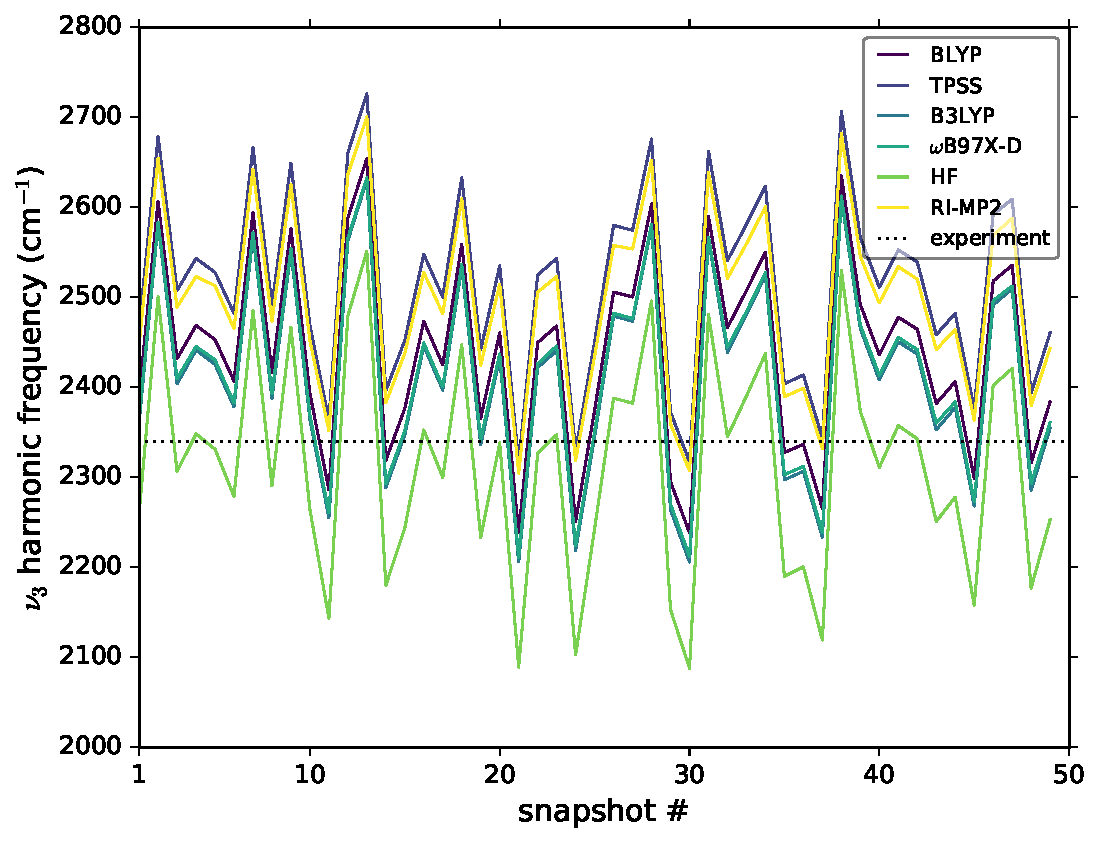
\includegraphics[width=\textwidth]{./paper_02/trajectory_frequencies_cc-pvtz.pdf}
  \caption[Instantaneous method and basis set dependence of MD snapshots]{Harmonic \(\nu_{3}\) frequencies (unscaled) for the first \num{50} (out of \num{1000}) snapshots calculated with different methods and the cc-pVTZ basis set (0 QM/256 MM).}
  \label{paper_02:fig:S4}
\end{figure}

\begin{table}
  \centering
  \caption[Effect of empirical and self-consistent dispersion corrections in ALMO-EDA]{Effect of empirical and self-consistent dispersion corrections on ALMO-decomposed interaction energies with comparison to SAPT0. Values are weighted averages over the same \num{15} snapshots as in Table~\ref{paper_02:tab:6}. Energies are reported in \si{\kcal\per\mole}.}
  \label{paper_02:tab:S3}
  \begin{tabular}{lccccc}
    \toprule
    method & \(E_{\text{frz}}\) & \(E_{\text{pol}}\) & \(E_{\text{CT}}\) & \(E_{\text{disp}}\) & \(E_{\text{tot}}\) \\
    \midrule
    HF/6-31G(d,p) & 0.082 & -1.303 & -0.102 & \textemdash{} & -1.323 \\
    B3LYP/6-31G(d,p) & 0.500 & -1.241 & -1.177 & \textemdash{} & -1.918 \\
    B3LYP-D2/6-31G(d,p) & 0.500 & -1.241 & -1.177 & -6.269 & -8.187 \\
    B3LYP-D3/6-31G(d,p) & 0.500 & -1.241 & -1.177 & -6.464 & -8.382 \\
    \(\omega\)B97X-D/6-31G(d,p) & -3.343 & -1.245 & -1.168 & \textemdash{} & -5.757 \\
    \(\omega\)B97X-D/cc-pVTZ & -3.114 & -1.617 & -1.209 & \textemdash{} & -5.941 \\
    \(\omega\)B97M-V/6-31G(d,p) & -5.494 & -1.256 & -0.523 & \textemdash{} & -7.274 \\
    \(\omega\)B97M-V/cc-pVTZ & -5.149 & -1.649 & -0.889 & \textemdash{} & -7.687 \\
    SAPT0/6-31G(d,p)/MCBS & -2.450 & -2.049 & -0.280 & -4.135 & -8.634 \\
    SAPT0/6-31G(d,p)/DCBS & 0.593 & -1.910 & & -4.714 & -6.031 \\
    SAPT0/jun-cc-pVTZ/MCBS & 1.009 & -2.473 & -0.203 & -6.930 & -8.394 \\
    SAPT0/jun-cc-pVTZ/DCBS & 1.469 & -2.382 & & -7.413 & -8.326 \\
    \bottomrule
  \end{tabular}
\end{table}

\begin{table}
  \centering
  \caption[Solvatochromic shift dependence on counterpoise corrections]{Effect of counterpoise correction on \ce{CO2} \(\nu_3\) harmonic frequency when applied during geometry optimization and/or the harmonic frequency calculation. Clusters are with 1 \ce{CO2}, 1 MMIM cation, and 1 anion. All frequencies are in \si{\wavenumber} and unscaled. The first column is from our previous paper. CP-corrected calculations were performed using Cuby as a driver for Turbomole 6.6 at the B3LYP/SP level with numerical integration grid 7.}
  \label{paper_02:tab:S4}
  CP-correction for geometry? / CP-correction for frequencies?
  \begin{tabular}{lcccc}
    \toprule
    anion & no/no & yes/no & no/yes & yes/yes \\
    \midrule
    \ce{TFA} & 2429.31 & 2428.05 & 2457.238 & 2440.879 \\
    \ce{SCN} (\ce{S}-coordinated) & 2430.24 & 2427.91 & 2445.642 & 2438.003 \\
    \ce{DCA} & 2430.47 & 2426.60 & 2436.113 & 2431.383 \\
    \ce{SCN} (\ce{N}-coordinated) & 2431.64 & 2427.95 & 2432.691 & 2437.876 \\
    \ce{TfO} & 2431.91 & 2428.95 & 2441.921 & 2443.665 \\
    \ce{BF4} & 2434.69 & 2431.48 & 2454.767 & 2450.890 \\
    \ce{Tf2N} & 2435.80 & 2431.49 & 2451.851 & 2441.309 \\
    \ce{PF6} & 2437.74 & 2432.58 & 2479.806 & 2469.473 \\
    \bottomrule
  \end{tabular}
\end{table}

\subsection{Potential Energy Surface Fitting}
\label{paper_02:ssec:SI5}

We fitted the discrete variable representation (DVR) of the Born-Oppenheimer potential energy surface of gas phase \ce{CO2} to a vibrational potential expanded in the local modes basis using a nonlinear least squares method. The potential energy expansion was truncated at fourth order, and off-diagonal fourth order terms (e.g.  \(c_{3}[(x - x_{0})^{2}(y - y_{0})^{2}]\)) were omitted, using the following form:

% \begin{dmath*}
\begin{equation*}
  \begin{split}
    V( x,y ) = & a_{1}( x - x_{0} )^{2} + a_{2}( y - y_{0} )^{2} + a_{3}( x - x_{0} )( y - y_{0} ) \\
    & + b_{1}( x - x_{0} )^{3} + b_{2}( y - y_{0} )^{3} + b_{3}[ ( x - x_{0} )^{2}( y - y_{0} ) + ( x - x_{0} )( y - y_{0} )^{2} ] \\
    & + c_{1}( x - x_{0} )^{4} + c_{2}( y - y_{0} )^{4}
  \end{split}
\end{equation*}
The resulting fit to the data was excellent (\(R^2 = 0.9997\)).

The force constants and internal coordinates were calculated (the F matrix) and multiplied by the appropriate mass weighting (G matrix). The product was diagonalized to obtain eigenvalues and eigenvectors, which give the normal modes and frequencies of the symmetric stretch (\(\nu_{1} = \SI{1377}{\wavenumber}\)) and antisymmetric stretch (\(\nu_{3} = \SI{2414}{\wavenumber}\)).

\begin{table}
  \centering
  \caption[Fit parameters for DVR PES]{Best fit parameters for DVR representation of the gas phase \ce{CO2} potential energy surface.}
  \label{paper_02:tab:S5}
  \begin{tabular}{cl}
    \toprule
    coefficient name & value (with 95\% confidence bound) \\
    \midrule
    \(a_1\) & \SI{1.8834 \pm 0.0178}{\hartree\per\angstrom\squared} \\
    \(a_2\) & \SI{1.8834 \pm 0.0178}{\hartree\per\angstrom\squared} \\
    \(a_3\) & \SI{0.3305 \pm 0.0087}{\hartree\per\angstrom\squared} \\
    \(b_1\) & \SI{-5.0013 \pm 0.1124}{\hartree\per\angstrom\cubed} \\
    \(b_2\) & \SI{-5.0005 \pm 0.1123}{\hartree\per\angstrom\cubed} \\
    \(b_3\) & \SI{-0.2205 \pm 0.0330}{\hartree\per\angstrom\cubed} \\
    \(c_1\) & \SI{6.3508 \pm 0.4031}{\hartree\per\angstrom\tothe{4}} \\
    \(c_2\) & \SI{6.3485 \pm 0.4031}{\hartree\per\angstrom\tothe{4}} \\
    \(x_0\) & \SI{1.1594 \pm 0.0009}{\angstrom} \\
    \(y_0\) & \SI{1.1594 \pm 0.0009}{\angstrom} \\
    \bottomrule
  \end{tabular}
\end{table}

\subsection{\texorpdfstring{\(\nu_{3}\)}{Asymmetric Stretch} Frequency Convergence with Increasing QM Size}
\label{paper_02:ssec:SI6}

To test the qualitative accuracy of the calculations using smaller QM regions, we examined the correlation between frequencies calculated with \(n = 0-5\) QM pairs and \num{6} QM pairs for each snapshot. The data were fitted using a linear regression analysis.

\begin{table}
  \centering
  \caption[Fit procedure results for DVR convergence]{Fitting results for correlation of QM/MM harmonic frequencies of \num{10} MD snapshots, with increasing numbers of anion-cation pairs (\(n_{\text{QM}}\)) treated quantum mechanically.}
  \label{paper_02:tab:S6}
  \footnotesize
  \begin{tabular}{ccl}
    \toprule
    \(n_{\text{QM}}(1)\) & \(n_{\text{QM}}(2)\) & fitting results \\
    \midrule
    0 & 6 &
            \begin{minipage}{4.5in}
\begin{verbatim}
                 Estimate   Standard Error
      Intercept  -20.915       1024.4
      Slope       1.0056      0.42745

  Root Mean Squared Error: 5.52
  R-squared: 0.409, Adjusted R-Squared: 0.335
\end{verbatim}
            \end{minipage} \\
    1 & 6 &
            \begin{minipage}{4.5in}
\begin{verbatim}
                 Estimate   Standard Error
      Intercept   60.512       593.34
      Slope      0.97282      0.24788

  Root Mean Squared Error: 4.2
  R-squared: 0.658, Adjusted R-Squared: 0.615
\end{verbatim}
            \end{minipage} \\
    2 & 6 &
            \begin{minipage}{4.5in}
\begin{verbatim}
                 Estimate   Standard Error
      Intercept   98.181          384
      Slope      0.95775      0.16053

  Root Mean Squared Error: 3.08
  R-squared: 0.816, Adjusted R-Squared: 0.794
\end{verbatim}
            \end{minipage} \\
    3 & 6 &
            \begin{minipage}{4.5in}
\begin{verbatim}
                 Estimate   Standard Error
      Intercept    173.5       306.89
      Slope      0.92667      0.12835

  Root Mean Squared Error: 2.62
  R-squared: 0.867, Adjusted R-Squared: 0.85
\end{verbatim}
            \end{minipage} \\
    4 & 6 &
            \begin{minipage}{4.5in}
\begin{verbatim}
                 Estimate   Standard Error
      Intercept   2.1463        172.16
      Slope      0.99837      0.072008

  Root Mean Squared Error: 1.44
  R-squared: 0.96, Adjusted R-Squared: 0.955
\end{verbatim}
            \end{minipage} \\
    5 & 6 &
            \begin{minipage}{4.5in}
\begin{verbatim}
                 Estimate   Standard Error
      Intercept  -26.98        85.681
      Slope      1.0111      0.035855

  Root Mean Squared Error: 0.717
  R-squared: 0.99, Adjusted R-Squared: 0.989
\end{verbatim}
            \end{minipage} \\
    \bottomrule
  \end{tabular}
\end{table}

\begin{figure}
  \centering
  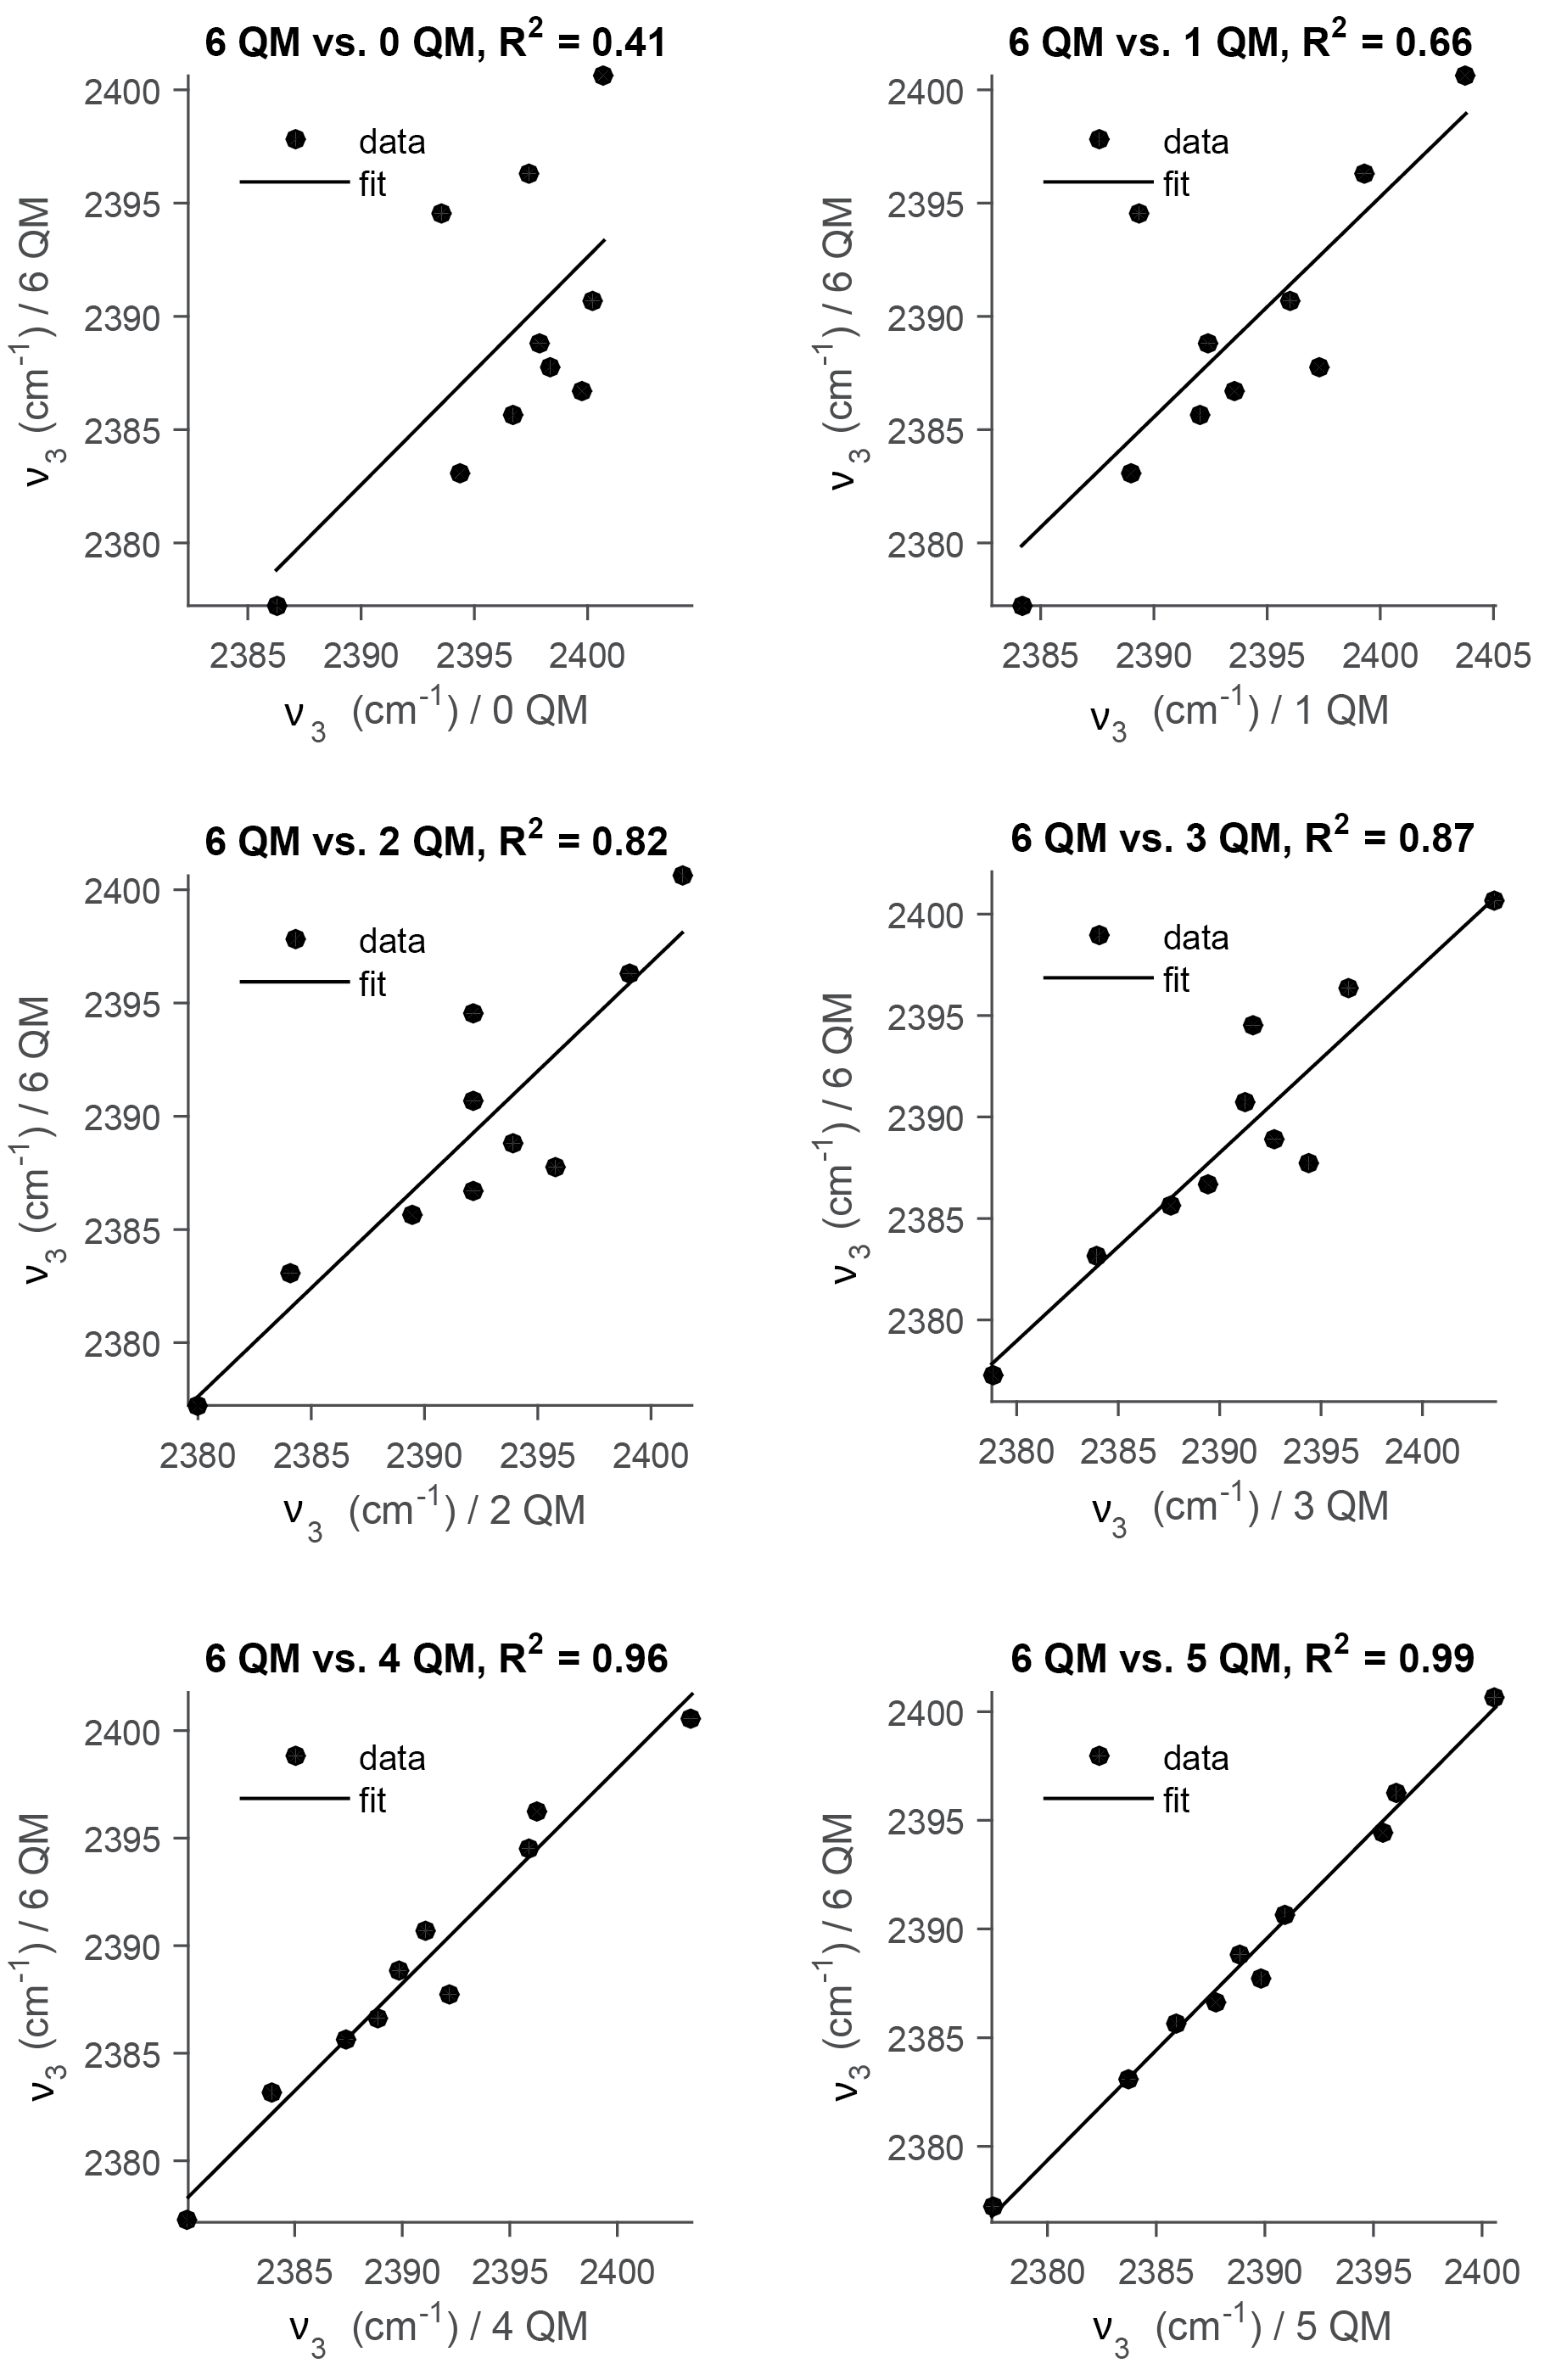
\includegraphics[scale=0.85]{./paper_02/figureS5.png}% TODO the png looks terribad
  \caption[Self-correlation of QM/MM frequencies with increasing QM region size]{Correlation plots for QM/MM harmonic frequencies of \num{10} MD snapshots, with increasing numbers of anion-cation pairs treated quantum mechanically.}
  \label{paper_02:fig:S5}
\end{figure}

% TODO contents of Excel spreadsheet

\chapter[Spectroscopic Map]{Modeling Carbon Dioxide Vibrational Frequencies in Ionic Liquids: II. Spectroscopic Map}
\label{ch:paper_03}

The text in this chapter has been adapted from

\section{\texorpdfstring{\caps{Summary}}{Summary}}

The primary challenge for connecting molecular dynamics (MD) simulations to linear and two-dimensional infrared (2D-IR) measurements is the calculation of the vibrational frequency for the chromophore of interest. Computing the vibrational frequency at each time step of the simulation with a quantum mechanical method like density functional theory (DFT) is generally prohibitively expensive. One approach to circumnavigate this problem is the use of spectroscopic maps. Spectroscopic maps are empirical relationships that correlate the frequency of interest to properties of the surrounding solvent that are readily accessible in the MD simulation. Here, we develop a spectroscopic map for the asymmetric stretch of \ce{CO2} in the 1-butyl-3-methylimidazolium hexafluorophosphate (\ce{[C4C1im][PF6]}) ionic liquid (IL). DFT is used to compute the vibrational frequency of \num{500} statistically independent \ce{CO2}-\ce{[C4C1im][PF6]} clusters extracted from an MD simulation. When the map was tested on a \num{500} different \ce{CO2}-\ce{[C4C1im][PF6]} clusters, the correlation coefficient between the benchmark frequencies and the predicted frequencies was \(R = 0.94\) and the root mean squared error was \SI{2.7}{\wavenumber}. The calculated distribution of frequencies also agrees well with experiment. The spectroscopic map required information about the \ce{CO2} angle, the electrostatics of the surrounding solvent, and the Lennard-Jones interaction between the \ce{CO2} and the IL. The contribution of each term in the map was investigated with symmetry-adapted perturbation theory (SAPT) calculations.

\section{\texorpdfstring{\caps{Introduction}}{Introduction}}
\label{paper_03:sec:I}

Ionic liquids (ILs) have attracted tremendous attention because of their properties as environmentally friendly alternatives to volatile organic solvents, and their applications involving the production, storage, and efficient utilization of energy.\cite{Karadas2010,wishartEES-09,Armand2009,Patel2012,baraACR-10} ILs exhibit unique physical properties relative to conventional liquids in terms of vapor pressure, viscosity, electrical and thermal conductivity, solubility of polar and nonpolar molecules, and melting point.\cite{baraACR-10,Crosthwaite2005,seki_effects_2010,Tokuda2005,anthonyJPCB-02} Moreover, these properties can be tuned to specific applications by chemically modifying the molecules that comprise the liquid. For example, by functionalizing the molecules of an IL to react with \ce{CO2}, improved design for preferentially separating \ce{CO2} from gas mixtures was achieved.\cite{anthonyJPCB-02,seoJPCB-14,shiflett_solubilities_2005,Gurkan2010,Cadena2004} Thus, ILs offer a promising new direction for the removal of environmentally harmful \ce{CO2} from postcombustion flue gas.

It is essential that the fundamental structure and dynamics of ILs be understood to aid in the design of new ILs for unique applications.  Unlike conventional solvents, ILs exhibit heterogeneous structure and dynamics that have profound implications for their physical properties.  Two-dimensional infrared (2D-IR) spectroscopy offers several unique advantages for interrogating the structure and dynamics of liquids because of its exquisite time and spatial resolution.\cite{Tamimi2016b,Ren2014,hamm_concepts_2011,khalil_coherent_2003} The spatial resolution results from the size of suitably chosen vibrational chromophores. The vibrational frequencies of these reporters depend sensitively on their local environment.\cite{Ren2014,levinson_phosphate_2011,choi_vibrational_2011,choiJCP-08,Lee2011,steinelCPL-04} As that local environment evolves, so too will the vibrational frequency of the probe \textemdash{} a process called spectral diffusion. 2D-IR spectroscopy measures these frequency fluctuation dynamics, which relate back to the intrinsic dynamics of the surroundings of the vibrational chromophore.

Recently, Brinzer \emph{et al}. have demonstrated that the asymmetric stretch of \ce{CO2} (\(\nu_3\) is an excellent vibrational reporter of its local environment in ILs.\cite{Brinzer2015} In particular, these experiments have established (1) that the asymmetric stretch of \ce{CO2} exhibits a significant solvatochromic shift with respect to the choice of anion in a series of imidazolium-based ILs, (2) that the \ce{CO2} vibrational population lifetime is sufficiently long to measure 2D-IR spectra on a \SI{100}{\pico\second} timescale, and (3) that the longest spectral diffusion timescale correlates empirically with the viscosity of the IL.\cite{Brinzer2015} Fayer and coworkers have also studied \ce{CO2} in ILs with 2D-IR spectroscopy, including detailed measurements and modeling of the rotational dynamics of \ce{CO2} and how this motion results in reorientational-induced spectral diffusion (RISD). Through analysis of polarization-selective 2D-IR measurements, the RISD contribution to the overall spectral diffusion process was quantified.\cite{Giammanco2016d,Giammanco2016} The RISD analysis assumed that shifts in the \ce{CO2} vibrational frequency were governed by a second-order Stark effect.

Among multidimensional vibrational spectroscopy's great successes was revealing the dynamics of hydrogen-bond network rearrangements in liquid water.\cite{asburyJCP-04,Asbury2004,Bakker2010,feckoSci-03,eavesPNAS-05,Gruenbaum2013,Jansen2010,loparoJCP-06a,loparoJCP-06b,Nibbering2004,Nicodemus2011,nicodemusJPCL-10,ramaseshaJCP-11,Roberts2009} However, these profound insights were only possible in conjunction with a robust theoretical effort.\cite{Lee2011,feckoSci-03,eavesPNAS-05,Gruenbaum2013,auer_hydrogen_2007,auer_ir_2008,corcelliJCP-04a,Hayashi2005,Jansen2009,Li2010,Chai2008,lin_water_2009-1,Paarmann2009,Pieniazek2009,shiJPCB-12,Skinner2009,Tainter2012,Yang2011,laageCPL-06,Laage2006,Laage2008,Laage2012,Laage2012a,Smith2005} Much of that theoretical effort focused on the development and application of empirical relationships connecting the instantaneous vibrational frequency of interest to structural properties \textemdash{} usually the electrostatics \textemdash{} of the surrounding condensed-phase environment.\cite{steinelCPL-04,auer_ir_2008,Li2006} Such relationships have come to be known as ``spectroscopic maps.'' With a spectroscopic map in hand, quantities such as the linear IR absorption spectrum, 2D-IR spectra, and the frequency fluctuation correlation function that quantifies spectral diffusion, can be readily calculated in a conventional molecular dynamics (MD) simulation.\cite{lin_water_2009-1,Li2006,Terranova2014} With the emergence of 2D-IR measurements on \ce{CO2} in ILs, there is ample motivation to develop a spectroscopic map for the asymmetric stretch of \ce{CO2} in an IL.

In paper I\cite{Berquist2017}, we developed and validated a robust quantum mechanics/molecular mechanics (QM/MM) protocol for calculating anharmonic \ce{CO2} vibrational frequencies in the 1-butyl-3-methylimidazolium hexafluorophosphate (\ce{[C4C1im][PF6]}) IL. Here, we have used the protocol to calculate the asymmetric stretch vibrational frequency of \ce{CO2} in 1000 statistically independent snapshots extracted from an MD simulation. For each frequency calculation, the \ce{CO2} molecule and two pairs of IL molecules are treated quantum mechanically with density functional theory (DFT). The rest of the solvent is included in the calculation as point charges that polarize the quantum mechanical region. The two-dimensional potential energy surface for the \ce{CO2} stretches is constructed on a \(12 \times 12\) grid and the resulting vibrational Schrödinger equation is solved using a discrete variable representation (DVR) method. Once the vibrational frequencies were calculated, \num{500} of these snapshots were used to parameterize the spectroscopic map and the other \num{500} snapshots were used to quantify the accuracy of the spectroscopic map.

Previous spectroscopic maps have primarily been based on electrostatics,\cite{choi_vibrational_2011,corcelliJCP-04a,ohJCP-08,corcelliJPCA-05,schmidt_pronounced_2005-1,blasiak_vibrational_2013,Basiak2014} but our initial quantum chemistry investigations\cite{Brinzer2015,Berquist2017} indicate that the antisymmetric stretch of \ce{CO2} is sensitive to other physical effects, including charge transfer, dispersion, exchange repulsion, and electrostatics. Accordingly, we found that a suitably accurate spectroscopic map could not be constructed using only electrostatic properties of the IL environment. Instead, we had to include both electrostatic and Lennard-Jones (LJ) terms in the map. Błasiak and Cho previously found that including dispersion interactions resulted in an improved spectroscopic map for the amide I vibration of \textit{N}-methylacetamide.\cite{Basiak2015} In addition, since the \ce{CO2} molecule was modeled as flexible in solution, the map also has a dependence on the \ce{CO2} bend angle whose contribution was investigated in detail.

Spectroscopic maps are inherently empirical and can, in principle, utilize any variable that is sufficiently correlated with the vibrational frequencies, even if that variable is not the cause of the vibrational frequency shifts. Therefore, the dual goals of this work are to develop and validate a spectroscopic map, and to understand how the causal variables manifest themselves in the map. To achieve the first goal, the average frequency and distribution of vibrational frequencies were compared to inhomogeneous vibrational spectra extracted from 2D-IR measurements. To achieve the second goal a selection of snapshots were analyzed with symmetry adapted perturbation theory (SAPT)\cite{Jeziorski1994,Hohenstein2010,Hohenstein2011} calculations.

In addition to the intermolecular interactions, \ce{CO2} has an important intramolecular degree of freedom, the bending mode. Our previous work\cite{Brinzer2015} has implicated the bending mode in the experimentally observed solvatochromic shifts. At room temperature, the bending mode has an energy of approximately \(3k_{B}T\), placing it in an intermediate regime where it is not clear if a flexible (classical) or a rigid (quantum) model should be more appropriate. To better understand the role of \ce{CO2} flexibility in the spectroscopic map, we calculated histograms of vibrational frequencies for a rigid (bond angle = \ang{180}) and a flexible model of \ce{CO2} in the \ce{[C4C1im][PF6]} IL. We also examined a third possibility where the \ce{CO2} is modeled as flexible in the MD simulation, but the bend angle is relaxed prior to applying the spectroscopic map.

The paper is organized as follows. In Section~\ref{paper_03:sec:II} the details of the MD simulations and the anharmonic vibrational frequency calculations are described. In Section~\ref{paper_03:sec:III}, the spectroscopic map is constructed. In Section~\ref{paper_03:sec:IV}, the spectroscopic map is validated by comparison to experiment. In Section~\ref{paper_03:sec:V}, the contributions of the electrostatic, exchange repulsion, and dispersive interactions in the spectroscopic map are analyzed with ALMO and SAPT calculations. Finally, in Section~\ref{paper_03:sec:VI} we provide some concluding remarks.

\section{\texorpdfstring{\caps{Computational Methods}}{Computational Methods}}
\label{paper_03:sec:II}

Molecular dynamics (MD) simulations were performed using the large-scale atomic/molecular massively parallel simulator (LAMMPS)\cite{Plimpton1995} with a time step of \SI{2}{\femto\second}. \num{256} ion pairs of \ce{[C4C1im][PF6]} and one molecule of \ce{CO2} were simulated at \SI{300}{\kelvin} in a cubic box with periodic boundary conditions. Previous studies have confirmed that \num{256} ion pairs is a sufficiently large simulation box to mitigate finite-size effects.\cite{andreussi_transport_2012} The original atomic coordinates and box size (\SI{45}{\angstrom}) were generated from a previous study of \ce{[C4C1im][PF6]} containing a single water solute, which had been subjected to a rigorous equilibration protocol.\cite{Terranova2014} The water was replaced with a \ce{CO2} solute, and was subjected to the following equilibration procedure: (1) \SI{1}{\nano\second} in the NVT ensemble at \SI{300}{\kelvin}, (2) heating to \SI{600}{\kelvin} over \SI{1}{\nano\second}, (3) cooling to \SI{300}{\kelvin} over \SI{1}{\nano\second}, (4) \SI{1}{\nano\second} in the NVT ensemble at \SI{300}{\kelvin}, and (5) \SI{1}{\nano\second} in the NVE ensemble. Production run trajectories were collected in the NVE ensemble. Energy conservation was excellent, with fits to the energy and temperature over \SI{10}{\nano\second} revealing slopes of \SI{3.3e-5}{\kcal\per\mole\per\pico\second} and \SI{9.8e-6}{\kelvin\per\pico\second}, respectively. All molecules were modeled as fully flexible except for bonds containing hydrogen, which were held fixed at their equilibrium lengths using the SHAKE algorithm.\cite{Forester1998,Ryckaert1977} Also, in certain cases (see below), the \ce{CO2} bond lengths and angle were held fixed at their equilibrium values using the LAMMPS rigid integrator.\cite{Plimpton1995} The force fields for \ce{[C4C1im][PF6]} were the same as in our previous simulation studies involving this IL.\cite{Terranova2014} Briefly, the bends, bonds, dihedrals, and Lennard-Jones parameters for \ce{[C4C1im]+} are from the generalized Amber force field (GAFF),\cite{sprenger_general_2015,wang_development_2004} and partial charges were obtained from DFT calculations.\cite{singh_combined_1986} The \ce{[PF6]-} force field parameters were from the work of Liu \emph{et al}.\cite{liu_refined_2004} Charges on the ions were scaled by \num{0.84} to empirically account for charge transfer and polarization effects in the IL.\cite{chaban_new_2011,schroder_comparing_2012} \ce{CO2} was modeled using the TraPPE force field, with additional terms developed by Perez-Blanco and Maginn for flexible bond lengths and angle.\cite{potoff_vaporliquid_2001,perez-blanco_molecular_2010} Lennard-Jones interactions were truncated at \SI{15}{\angstrom} and the long-ranged electrostatics were computed using particle-mesh Ewald summation with a \SI{15}{\angstrom} real space cutoff.\cite{darden_particle_1993}

In order to create a spectroscopic map, \num{1000} statistically independent snapshots separated by \SI{50}{\pico\second} were collected from a pair of \SI{50}{\nano\second} simulations, one with a fully flexible \ce{CO2} and a second with a fully rigid \ce{CO2}. For each snapshot, the Born-Oppenheimer potential energy surface (PES) for \ce{CO2} stretching modes was obtained from single point energy calculations performed as the \ce{CO} bond lengths were stretched from \SIrange{0.955}{1.45}{\angstrom} in \SI{0.045}{\angstrom} steps. During these calculations, the nearest two pairs of ions by center of mass were included quantum mechanically, and the remaining ions within \SI{20}{\angstrom} were included as their point charges from the MD force field. The resulting PES was included in a discretized construction of the Hamiltonian for \ce{CO} stretches, which was then diagonalized, producing the asymmetric stretch frequency. More details about this method can be found in paper 1 of this series. Least squares multiple linear regression was used to empirically fit the electric field due to the anions and cations along the \ce{CO} bonds and the Lennard-Jones potential energy on the \ce{CO2} carbon and oxygens to the asymmetric stretch of \ce{CO2} for \num{500} of the flexible snapshots, and the accuracy of the resulting fit was tested using the remaining \num{500} snapshots. \num{500} of the rigid snapshots were used as a secondary test set. This is described in more detail in section~\ref{paper_03:sec:IV}. In certain cases, the \ce{CO2} angle from the flexible simulation was relaxed holding all other degrees-of-freedom and the \ce{CO2} center of mass fixed prior to vibrational frequency calculations for further analysis. This is discussed further in Section~\ref{paper_03:ssec:V-B}.

\section{\texorpdfstring{\caps{Spectroscopic Map for \ce{CO2} Vibrations}}{Spectroscopic Map for CO2 Vibrations}}
\label{paper_03:sec:III}

Empirical spectroscopic maps relate the instantaneous vibrational frequency of an IR reporter to properties of its surroundings that can be readily accessed in MD simulations.\cite{lin_water_2009-1,Terranova2014,malolepsza_empirical_2014} Once a spectroscopic map has been parameterized, it can be used to calculate IR absorption spectra, 2D-IR spectra, and frequency fluctuation time correlation functions from a MD simulation. For the asymmetric stretch of \ce{CO2} in \ce{[C4C1im][PF6]}, we were unable to obtain a suitably accurate spectroscopic map from electrostatics alone. Instead, we needed to include information about the \ce{CO2} bend angle, as well as the Lennard-Jones (LJ) interactions between \ce{CO2} and the surrounding IL. The spectroscopic map has the following form

\begin{equation}
  \label{paper_03:eq:1}
  \omega_{a} = \omega_{g} + \Delta\omega_{\theta} + \Delta\omega_{\text{solvent}}
\end{equation}

where \(\omega_{a}\) is the predicted \ce{CO2} asymmetric stretch vibrational frequency, \(\omega_{g}\) is the experimental gas phase frequency (\SI{2349.1}{\wavenumber}), \(\Delta\omega_{\theta}\) is the dependence of the frequency on the \ce{OCO} bend angle, and \(\Delta\omega_{\text{solvent}}\) captures the change in the vibrational frequency due to interactions with the IL solvent. Figure~\ref{paper_03:fig3} shows the dependence of the \ce{CO2} asymmetric stretch vibrational frequency on the \ce{OCO} angle, \(\theta\), calculated for \ce{CO2} isolated in the gas-phase. The calculated data are fit exquisitely well (\(R^{2} = 0.999\)) by the single-parameter function

\begin{equation}
  \label{paper_03:eq:2}
  \Delta\omega_{\theta} = a(1 + \cos{\theta})
\end{equation}

where \(a = \SI{-1160.9}{\wavenumber}\).

Figure~\ref{paper_03:fig3} also shows the vibrational frequency of \num{500} statistically independent \ce{CO2}/\ce{[C4C1im][PF6]} snapshots. The vibrational frequencies were calculated using the DVR approach described in paper 1 in this series. In these calculations, the \ce{CO2} and the closest two pairs of \ce{[C4C1im][PF6]} molecules \textemdash{} determined using the distance between the center-of-mass of the IL molecule and the \ce{CO2} carbon atom \textemdash{} were treated quantum mechanically at the B3LYP/6-311++G(d,p) level of theory. Any IL molecule whose center-of-mass was within \SI{20}{\angstrom} was modeled using its molecular mechanics partial atomic charges, which then polarize the quantum mechanical region. IL molecules were added to the molecular mechanics region in pairs to maintain charge neutrality. The overall trend in the vibrational frequencies roughly follows the angle dependence in the gas phase, but there is significant scatter due to interactions with the IL.

A map for the solvent effects on the asymmetric \ce{CO2} vibrational frequency was constructed assuming the following form,

\begin{equation}
  \label{paper_03:eq:3}
  \Delta\omega_{\text{solvent}} = b_{1}E_{\ce{O}}^{\text{Cation}} + b_{2}E_{\ce{O}}^{\text{Anion}} + c_{1}U_{\ce{O}} + c_{2}U_{\ce{C}}
\end{equation}

where \(E\) and \(U\) represent contributions from the electric field and Lennard-Jones (LJ) interactions with the solvent, respectively. The subscript, \ce{C} or \ce{O}, indicates whether the interaction is computed at the location of the \ce{CO2} central carbon or at the oxygen atoms. For \(E_{\ce{O}}\) and \(U_{\ce{O}}\), the value used in Eq.~(\ref{paper_03:eq:3}) is the average for the two \ce{CO2} oxygen sites. The LJ interaction is computed using the expression,

\begin{equation}
  \label{paper_03:eq:4}
  U = \ \sum_{j}^{}\varepsilon_{j}\left\lbrack \left( \frac{\sigma_{j}}{r_{j}} \right)^{12} - \left( \frac{\sigma_{j}}{r_{j}} \right)^{6} \right\rbrack
\end{equation}

where the sum is over all atoms in the surrounding liquid, \(\varepsilon_{j}\) and \(\sigma_{j}\) are the LJ parameters for the atom, and \(r_{j}\) is the distance to the atom. The electric fields are calculated with respect to the oxygen atoms of \ce{CO2} and are projected along the relevant \ce{CO} bond,

\begin{equation}
  \label{paper_03:eq:5}
  E = {\hat{r}}_{\ce{CO}} \cdot \sum_{j}^{}\frac{q_{j}{\hat{r}}_{j}}{r_{j}^{2}}
\end{equation}

where the sum is over all relevant atoms in in the surrounding liquid (i.e. those associated with the cations for \(E_{\ce{O}}^{\text{Cation}}\) and those associated with the anions for \(E_{\ce{O}}^{\text{Anion}}\)), \(q_{j}\) is the partial atomic charge, \(r_{j}\) is the distance to the charge, \({\hat{r}}_{j}\) is a unit-vector directed toward the site of the charge, and \({\hat{r}}_{\mathrm{\text{CO}}}\) is a unit vector from the carbon atom of \ce{CO2} to the relevant oxygen atom. Long range electrostatics are corrected using the damped shifted force method.\cite{fennell_is_2006}

The four parameters, \(b_{1}\), \(b_{2}\), \(c_{1}\), and \(c_{2}\), in Eq.~(\ref{paper_03:eq:3}) were determined empirically by applying multiple linear regression using the \num{500} calculated frequencies in the training set (Table~\ref{paper_03:tab1}). The quality of the fit was evaluated using the \num{500} different frequencies contained in the test set (Figure~\ref{paper_03:fig2}). The root-mean-square (RMS) deviation between the test set frequencies and those predicted by Eq.~(\ref{paper_03:eq:3}) was \SI{2.7}{\wavenumber}, and the value of correlation coefficient for the fit was \(R = 0.94\). By both metrics, the quality of the spectroscopic map for predicting the \ce{CO2} asymmetric stretch vibrational frequencies in the \ce{[C4C1im][PF6]} IL is as good or better than previously published maps for other vibrational reporters in conventional solvents. Additionally, when \num{500} rigid \ce{CO2} snapshots are used as the test set, the same level of accuracy is obtained.

The Condon approximation, that the magnitude of the transition dipole moment is independent of the vibrational frequency of a mode, fails for some solutes that interact in a strong local way with their environment. The most important example is the \ce{OH} stretch of liquid water. The hydrogen bonds in water polarize the OH bond, increasing the oscillator strength on the red side of the vibrational band, which has a significant effect on the IR absorption line shape.\cite{corcelliJPCA-05,schmidt_pronounced_2005-1,loparoCP-07} Similar to the hydrogen bonding of water, the strong local interactions of \ce{CO2} with the ionic liquid anion could, in principle, cause the Condon approximation to fail. However, we find that the Condon approximation for the main band is adequate (Figure~\ref{paper_03:fig3}). We calculated the transition dipole moment integral, \(\mu_{01}\), of the asymmetric stretch of \ce{CO2} in \num{1000} \ce{CO2}-\ce{[C4C1im][PF6]} clusters. The details of the transition dipole moment integral calculations are provided in the Supporting Information (SI). A plot of \(\mu_{01}\) scaled by \(\mu_{01}^{g}\), the transition dipole moment integral of the asymmetric stretch of \ce{CO2} in the gas-phase, versus the asymmetric stretch vibrational frequency, \(\omega_{a}\), has a slope close to zero. This confirms that it is reasonable to regard the transition dipole as a constant factor that scales the intensity of linear and non-linear spectra but does not modify their shapes. As a result, we do not treat the environmental dependence of the transition dipole moment in our spectroscopic map; we need only treat the vibrational frequencies.

\section{\texorpdfstring{\caps{Physical Interpretation of the Spectroscopic Map}}{Physical Interpretation of the Spectroscopic Map}}
\label{paper_03:sec:IV}

The average contribution to the \ce{CO2} asymmetric stretch vibrational frequency from each of the map components is listed in Table~\ref{paper_03:tab2}. This data demonstrates that the Lennard-Jones potential energy is an important predictor of the vibrational frequency of \ce{CO2} solvated in \ce{[C4C1im][PF6]}, while the electrostatic potential plays a secondary role. This contrasts many prior spectroscopic maps where solvatochromic frequency shifts were based purely on the electrostatics of the environment.\cite{lin_water_2009-1,ohJCP-08,Miller2009} This finding is perhaps surprising at first, because one might expect electrostatics to dominate the interactions of a solute with charged solvent molecules; however, one has to consider that (1) \ce{CO2} is not dipolar or charged, and as such will not interact with uniform electric fields very strongly, and (2) the ionic liquid, particularly the \ce{[C4C1im]+} butyl tails, have large domains where the dominant interactions are dispersive. These points make it conceivable that van der Waals effects dominate the \ce{CO2}-IL interaction.

To further unravel the origin of the impact of \ce{CO2}-IL interactions on the vibrational signature of \ce{CO2}, we use the fact that the LJ contributions to the spectroscopic map can be further decomposed. In particular, we separate the LJ term into its repulsive (\({\sim r}^{-12}\)) and attractive (\(\sim r^{-6}\)) contributions (Table~\ref{paper_03:tab2}). We find that the attractive and repulsive LJ terms contribute \SI{-7.0}{\wavenumber} and \SI{+4.9}{\wavenumber}, respectively, to the overall LJ vibrational shift of \SI{-2.1}{\wavenumber}. The large contribution from the repulsive LJ term is yet another surprise. To aid in identifying the physical origins of the large repulsive LJ contribution, we performed symmetry adapted perturbation theory (SAPT)\cite{Hohenstein2011} calculations that decompose the total interaction energy into physically meaningful components. This analysis should be contrasted with the empirical spectroscopic map, where a good fit implies correlation but not necessarily causation. Our SAPT calculations yield energy contributions, but it should nevertheless be possible to estimate the relative importance of different interactions for vibrational frequencies. The SAPT decomposition supports the previous discussion in that electrostatic interactions (electrostatics, induction) plus the exchange (exchange repulsion, exchange-induction) roughly cancel (total \SI{-1.3}{\kcal\per\mole}), whereas dispersive interactions dominate the interaction (total \SI{-4.7}{\kcal\per\mole} from dispersion plus exchange-dispersion). However, the SAPT data also reveals that exchange-dispersion (the repulsive dispersion part) is over an order of magnitude smaller than the attractive dispersion contribution (10.1\% of the total dispersion interaction). This result has to be contrasted with the \textasciitilde{}40\% contribution that the repulsive LJ potential makes to the vibrations. Since the repulsive LJ contribution is the dominant repulsive interaction incorporated in our model, the SAPT results suggest that the repulsive part of the LJ potential fits an agglomerate of exchange (Pauli) repulsion stemming from charge overlap (74.7\% of the repulsive interactions), exchange induction (20.7\%) plus exchange dispersion (4.6\%).

It is likely that LJ components will be an important component of a spectroscopic map for any neutral and nonpolar solute, or any solvent where dispersive interactions, quantum effects (Pauli exchange, for instance), or higher order electrostatic interactions are particularly important. In our case, it seems logical that a higher potential at the carbon would increase the optimal length of the CO bonds, thus decreasing the local mode and normal mode frequencies. Meanwhile, at the oxygen, a larger potential would generally shorten the bond, increasing the frequency. A similar finding was observed by Brinzer \emph{et al}.\cite{Brinzer2015} However, these components only allow the \ce{CO2} vibration to respond to local effects \textemdash{} the electric field components allow it to respond to longer-range interactions. As in prior works for different solvents and solutes, the coefficients for the two electric field components are different from each other, in this case by a substantial margin. It has been previously established that \ce{CO2} interacts with the anions more strongly than with the cations in an ionic liquid.\cite{Cadena2004,akiJPCB-04,anthonyJPCB-05,Muldoon2007a,houIECR-07,ramdinIECR-12} This is reflected in the magnitude of the coefficients related to the two components, and in their average frequency contribution (Tables~\ref{paper_03:tab1}~and~\ref{paper_03:tab2}). In particular, \ce{CO2} is a Lewis acid and should generally interact with negatively charged moieties differently from positively charged ones.

\section{\texorpdfstring{\caps{Validation}}{Validation}}
\label{paper_03:sec:V}

\subsection{Experimental Frequency Distribution}
\label{paper_03:ssec:V-A}

In order to compare our calculated distributions of \ce{CO2} vibrational frequencies with experiment, we must account for the effects that broaden or narrow the IR absorption line shape beyond the underlying distribution of frequencies. The finite population lifetime of the asymmetric stretch vibration, reorientation of the \ce{CO2} molecule, and a variety of other effects can broaden the absorption spectrum. On the other hand, fast dynamics can narrow the absorption spectrum (i.e. motional narrowing). A faithful comparison to experiment requires a deconvolution of these contributions to estimate the range of instantaneous frequencies experienced by \ce{CO2}.

2D-IR spectra contain sufficient information to recover the distribution of frequencies, which would be difficult to extract from the linear IR absorption spectrum alone.\cite{Brinzer2015} Within the Kubo multi-exponential ansatz, the width of the frequency distribution is determined by the frequency fluctuation correlation function

\begin{equation}
  \label{paper_03:eq:6}
  \Braket{\delta\omega(t)\delta\omega(0)} = \sum_{i}^{N} \Delta_{i}^{2}\exp\left( - \frac{t}{\tau_{i}} \right)
\end{equation}

where \(\Delta_{i}^{2}\) are the variances of frequency modulations, and \(\tau_{i}\) are the timescales for the respective frequency fluctuations. The width of the frequency distribution is the sum of squares of the different broadening processes

\begin{equation}
  \label{paper_03:eq:7}
  \Braket{\delta\omega^{2}} = \sum_{i}^{N} \Delta_{i}^{2}
\end{equation}

The contribution of homogeneous processes whose frequency fluctuations are too fast to be resolved (specifically when \(\Delta_{i}\tau_{i} \ll 1\)) can be approximated as \(\delta(t)\Delta_{H}^{2}\tau_{H}\), which results in a frequency correlation function:

\begin{equation}
  \label{paper_03:eq:8}
  \Braket{\delta\omega(t)\delta\omega(0)} = \delta(t)\Delta_{H}^{2}\tau_{H} + \sum_{i}^{N - 1}{\Delta_{i}^{2}\exp\left( - \frac{t}{\tau_{i}} \right)} = \frac{\delta(t)}{T_{2}^{*}} + \sum_{i}^{N - 1}{\Delta_{i}^{2}\exp\left( - \frac{t}{\tau_{i}} \right)}
\end{equation}

where \(T_{2}^{*} \equiv \left( \Delta_{H}^{2}\tau_{H} \right)^{- 1}\) is the pure dephasing time and \(\delta(t)\) is the Dirac delta function. The pure dephasing time depends on the variance of the fast frequency fluctuations, \(\Delta_{H}^{2}\), and the correlation time for fast motions, \(\tau_{H}\), and the two parameters cannot be independently determined. Analyzing the change in shape of the 2D-IR spectra as a function of the waiting time can directly determine the magnitude of frequency modulations related to the sum of exponential decays, \(\sum_{i}^{N - 1}\Delta_{i}^{2}\), in Eq.~(\ref{paper_03:eq:8}). For \ce{CO2} in \ce{[C4C1im][PF6]} this sum is approximately \SI{2}{\wavenumber}.\cite{Brinzer2015}

Determining the magnitude of frequency modulations that give rise to the first term in Eq.~(\ref{paper_03:eq:8}) is more complicated. The pure dephasing time (\(T_{2}^{*}\)) is only one contributor to the experimentally determined dephasing time (\(T_{2}\)), which also depends on the population (\(T_{1}\)), and reorientational (\(T_{or}\)) motions of the molecule

\begin{equation}
  \label{paper_03:eq:9}
  \frac{1}{T_{2}}\  = \frac{1}{T_{2}^{*}} + \frac{1}{2T_{1}} + \frac{1}{3T_{or}}
\end{equation}

The experimental dephasing time, \(T_{2}\), of the asymmetric stretch of \ce{CO2} in the \ce{[C4C1im][PF6]} IL is \SI{3.3}{\pico\second}.\cite{Brinzer2015} Since the experiment was performed in an all-parallel polarization, we cannot unambiguously determine the population and orientation relaxation times. We can estimate them, however, based on the rate of signal decay and the orientational correlation functions determined in a similar ionic liquid.\cite{Giammanco2016d,Giammanco2016} Estimates of \(T_{1} = \SI{20}{\pico\second}\) and \(T_{\mathrm{or}} = \SI{10}{\pico\second}\), suggest that vast majority contribution to \(T_{2}\) for \ce{CO2} in \ce{[C4C1im][PF6]} comes from pure dephasing. Population relaxation and orientational relaxation have a minor effect on the total dephasing time. We estimate a pure dephasing time of \(T_{2}^{*} = \SI{4}{\pico\second}\).

Finally, the variance of the frequency fluctuations, \(\Delta_{H}^{2}\), can be limited to a range by physical constraints on the values of \(\tau_{H}\). The lower limit on \(\tau_{H}\) is governed by the inertial motions of \ce{CO2} and its ionic liquid solvent shells. The timescale of the inertial response in liquid water is in the sub-\SI{60}{\femto\second} range, while that of acetonitrile is \SI{70}{\femto\second}.\cite{feckoSci-03,stengerPRL-01,Rosenthal1991} Using \SI{70}{\femto\second} as a lower limit for \(\tau_{H}\) places an upper limit on \(\Delta_{H}\) of \SI{9.7}{\wavenumber}. Fits to analytical response functions suggests that \(\Delta_{H}\ \tau_{H} \approx 0.2\) is a reasonable estimate of the dynamics that can be resolved using global fitting of the experimental data, which gives an upper limit on \(\tau_{H}\) of \SI{200}{\femto\second}, with a corresponding lower limit on \(\Delta_{H}\) of \SI{6}{\wavenumber}. Our estimate for the homogeneous width is thus, \(6 < \Delta_{H} < \SI{10}{\wavenumber}\). Combining the broadening due to fast and slow motions, the experimentally estimated total frequency width for \ce{CO2} in \ce{[C4C1im][PF6]} is between \SIrange{6.3}{10.2}{\wavenumber} (Figure~\ref{paper_03:fig4}).

\subsection{Calculated Frequency Distributions}
\label{paper_03:ssec:V-B}

Figure~\ref{paper_03:fig5}a shows the distribution of \ce{CO2} asymmetric stretch vibrational frequencies computed using the spectroscopic map for 1000 statistically independent snapshots collected from an MD simulation of flexible \ce{CO2} in \ce{[C4C1im][PF6]}. These are the same snapshots that were used to parametrize and validate the spectroscopic map in Section III. The distribution is peaked at approximately \SI{2344}{\wavenumber} and its standard deviation is \SI{7.4}{\wavenumber}. Both of these values are in reasonable agreement with experiment (\SI{2342.5}{\wavenumber} and \SIrange{6.3}{10.2}{\wavenumber}). Qualitatively, the distribution exhibits a significant asymmetry with a mean frequency of \SI{2339.9}{\wavenumber} that is about \SI{4}{\wavenumber} to the red of the peak frequency. The experimental IR absorption line shape, however, does not show signs of such asymmetry in the underlying distribution of frequencies.

The source of the asymmetry in the distribution of frequencies in Figure~\ref{paper_03:fig5}a is the contribution to the spectroscopic map from the \ce{CO2} bend angle, Eq.~(\ref{paper_03:eq:2}). This is illustrated in Figure~\ref{paper_03:fig5}c, where we have calculated the distribution of \ce{CO2} asymmetric stretch vibrational frequencies for 1000 statistically independent snapshots collected from an MD simulation of rigid \ce{CO2} in \ce{[C4C1im][PF6]}. Since the \ce{CO2} molecule has an angle of \ang{180} in each of the snapshots, the contribution to the calculated vibrational frequency from the \ce{CO2} bend angle is zero. The resulting distribution is correctly symmetric with a mean frequency of \SI{2346.5}{\wavenumber} and a standard deviation of \SI{2.3}{\wavenumber}. The calculated distribution is centered \SI{4}{\wavenumber} to the blue of the experimental distribution, and it is narrower than the lower estimate of the experimental distribution by \SI{4}{\wavenumber}.

The results in Figure~\ref{paper_03:fig5}a~and~\ref{paper_03:fig5}c represent two extremes \textemdash{} one where the \ce{CO2} bend is treated classically (Figure~\ref{paper_03:fig5}a) and another where the \ce{CO2} bend is effectively neglected (Figure~\ref{paper_03:fig5}c). When the \ce{CO2} bend is classical, it is assumed that the \ce{CO2} asymmetric stretch vibrational frequency depends on the instantaneous value of the bend angle, Figure~\ref{paper_03:fig1} and Eq.~(\ref{paper_03:eq:2}). However, the asymmetric distribution suggests that this approach is incorrect. In fact, a simple thought experiment reinforces the problems associated with regarding the \ce{CO2} bend as a classical variable. Consider a non-rotating \ce{CO2} molecule isolated in the gas-phase. If all of the vibrations of the \ce{CO2} molecule are quantum mechanical, the distribution of each of the four vibrations is a delta function. However, if the bend is classical with a kinetic energy commensurate with room temperature, the distribution of asymmetric stretch vibrational frequencies will incorrectly have a finite width. One solution to this conundrum is to adopt a fully quantum mechanical treatment of the \ce{CO2} vibrations. This would require the construction of a four-dimensional potential energy surface for each of the 1000 benchmark \ce{CO2}-\ce{[C4C1im][PF6]} clusters, which is computationally intractable.

An alternate strategy is to treat the influence of the \ce{CO2} bend on the asymmetric stretch vibrational frequency using first-order perturbation theory. Instead of utilizing the instantaneous \ce{CO2} angle in Eq.~(\ref{paper_03:eq:2}), \(\theta\), we would instead use the average angle, \(\Braket{\theta} = \Braket{ \varphi_{0} | \theta | \varphi_{0} }\), where \(\varphi_{0}(\theta)\) is the ground vibrational wavefunction for the \ce{CO2} bend. Returning to the \ce{CO2} in the gas-phase thought experiment, the average angle is constant and equal to 180º. Thus, there would correctly be no contribution to \ce{CO2} asymmetric stretch vibrational frequency. In contrast, the instantaneous average bend angle will fluctuate away from \ang{180} in an IL because of asymmetric solvation by the solvent. Of course, we do not have access to vibrational wavefunction for the \ce{CO2} bend for the benchmark \ce{CO2}-\ce{[C4C1im][PF6]} clusters, nor when we wanted to utilize the spectroscopic map to analyze an MD simulation. An additional approximation is necessary. If we were to regard the \ce{CO2} bend as harmonic, then the average angle is given by the instantaneous distortion of the \ce{CO2} geometry by the environment. For the benchmark clusters, the geometry distortion can be determined by optimizing the geometry of the \ce{CO2} molecule using the classical MD force field and a conjugate gradient minimization while holding fixed both the center-of-mass of the \ce{CO2}, as well as the configuration of the IL solvent. The map is then used to calculate the vibrational frequency for the relaxed snapshot.

Figure~\ref{paper_03:fig5}b shows the distribution of \ce{CO2} asymmetric stretch vibrational frequencies computed using the spectroscopic map for \num{1000} statistically independent snapshots collected from an MD simulation of flexible \ce{CO2} in \ce{[C4C1im][PF6]} where the \ce{CO2} bend angle has been relaxed. On average, the relaxed bend angle is \ang{178.4}, and the distribution of frequencies is nearly symmetric with a mean frequency of \SI{2343.8}{\wavenumber} and a standard deviation of \SI{2.4}{\wavenumber}. The mean frequency is in excellent agreement with experiment and differs by only \SI{1.3}{\wavenumber}. Note that this agreement implies that the spectroscopic map is able to accurately capture the solvatochromic shift of the \ce{CO2} asymmetric stretch vibrational frequency from the gas-phase to the \ce{[C4C1im][PF6]} IL. The width of the distribution is too narrow compared to the estimated width of the experimental distribution of \SIrange{6.3}{10.2}{\wavenumber}. There are several possible sources for the discrepancy in the width of the distribution, including inaccuracies associated with the approximate perturbative approach for the effect of the bend on the asymmetric stretch frequency. However, the overall agreement with experiment is encouraging.

It is instructive to compare the distributions in Figures~\ref{paper_03:fig5}b (relaxed \ce{CO2}) and \ref{paper_03:fig5}c (rigid \ce{CO2}). Both distributions are symmetric and they have nearly the same widths: \SI{2.4}{\wavenumber} and \SI{2.3}{\wavenumber}, respectively. Thus, within the approximate perturbative approach, the bend has very little influence on the width of the distribution. The averages of the distributions differ more significantly: \SI{2343.8}{\wavenumber} and \SI{2346.5}{\wavenumber}, respectively. The bend shifts the distribution to the red and into better agreement with experiment. Overall, the role of the bend is relatively minor resulting in a redshift of the distribution by \SI{2.7}{\wavenumber}. These results suggest several options for how the bend is treated when the map is applied in conjunction with MD simulations to understand the spectroscopy and spectral diffusion dynamics of \ce{CO2} in the \ce{[C4C1im][PF6]} IL in Paper III\cite{Brinzer2018} in this series. The simplest strategy is to hold the \ce{CO2} rigid and to shift the calculated frequencies by \SI{2.7}{\wavenumber}. In essence, this would just account for the average effect of the \ce{CO2} angle on the asymmetric stretch frequencies. A more computationally intensive strategy is a simulation with \ce{CO2} flexible, but where the geometry of the \ce{CO2} is optimized using the classical force field. The efficacy of these approaches will be evaluated in Paper III\cite{Brinzer2018}.

\section{\texorpdfstring{\caps{Conclusions}}{Conclusions}}
\label{paper_03:sec:VI}

% TODO at the minimum, this passage is missing things from the final paper!
In this paper we have developed and validated a spectroscopic map that is the foundation for a molecular interpretation of ultrafast vibrational spectroscopy of \ce{CO2} in ionic liquids. In addition, we have established important insights into the solvatochromic shift of the \ce{CO2} asymmetric stretch vibrational frequency in ILs. We analyzed the physical origin of the vibrational frequency shifts using SAPT energy decomposition schemes. Unlike other vibrational chromophores, electrostatics alone poorly predict the vibrational frequency. While the most important contributor to the electrostatic part of the spectroscopic map is the field from the anion, both attractive dispersion interactions and repulsive charge overlap forces (Pauli repulsion) play additional important roles. Finally, while the \ce{CO2} bend angle influences the asymmetric stretch frequency, we have shown that the geometry of the \ce{CO2} molecule is only slightly perturbed by the IL, so regarding the \ce{CO2} as rigid is generally sufficient to capture the structural relaxation of the IL relative to the \ce{CO2}.

\section{\texorpdfstring{\caps{Acknowledgements}}{Acknowledgements}}

The authors thank Prof. Kenneth D. Jordan for helpful discussions. SAC is grateful for financial support from the National Science Foundation (CHE-1565471), the American Chemical Society Petroleum Research Fund (52648-ND6), and the Sustainable Energy Initiative at the University of Notre Dame. SAC and CAD are also thankful for high performance computing resources and support from the Center for Research Computing at the University of Notre Dame. Computational resources were also provided by the Center for Simulation and Modeling at the University of Pittsburgh. SGR acknowledges financial support from the National Science Foundation (CHE-1454105).

\begin{table}[H]
  \centering
  \caption[Parameters of the spectroscopic map]{Parameters of the spectroscopic map for the \ce{CO2} asymmetric stretch frequency in \ce{[C4C1im][PF6]}.  This map predicts the \ce{CO2} with a regression coefficient \(R = 0.94\) and a root mean squared error of \SI{2.7}{\wavenumber}. The average shift, \(\Braket{\Delta\omega}\), and standard deviation, \(\sigma(\Delta\omega)\), are reported for each term in the map.}
  \label{paper_03:tab1}
  \begin{longtable}[]{@{}cccc@{}}
    \toprule
    & & \(\Braket{\Delta\omega}\) (\si{\wavenumber}) & \(\sigma(\Delta\omega)\) (\si{\wavenumber})\tabularnewline
    \midrule
    \endhead
    \(\omega_{g}\) & \SI{2349.1}{\wavenumber} & 0.0 & 0.0\tabularnewline
    \(a\) & \SI{-1160.9}{\wavenumber} & -6.6 & 7.0\tabularnewline
    \(b_1\) & \SI{64.4}{\wavenumber\per\au} & -0.1 & 0.4\tabularnewline
    \(b_2\) & \SI{93.2}{\wavenumber\per\au} & -1.8 & 0.7\tabularnewline
    \(c_1\) & \SI{4.70}{\wavenumber\per\kcal\mole} & -9.5 & 2.0\tabularnewline
    \(c_2\) & \SI{-3.55}{\wavenumber\per\kcal\mole} & 7.3 & 2.1\tabularnewline
    \bottomrule
  \end{longtable}
\end{table}

\begin{table}[H]
  \centering
  \caption{Decomposition of the average LJ contribution to the spectroscopic map for the \ce{CO2} asymmetric stretch frequency in \ce{[C4C1im][PF6]} into attractive and repulsive components.}
  \label{paper_03:tab2}
  \begin{longtable}[]{@{}ccc@{}}
    \toprule
    LJ Component & Site & \(\Braket{\Delta\omega}\) (\si{\wavenumber})\tabularnewline
    \midrule
    \endhead
    Attractive & O & -21.7\tabularnewline
    & C & 14.8\tabularnewline
    & Sum & -6.9\tabularnewline
    Repulsive & O & 12.3\tabularnewline
    & C & -7.4\tabularnewline
    & Sum & 4.9\tabularnewline
    Total & O & -9.4\tabularnewline
    & C & 7.3\tabularnewline
    & Sum & -2.1\tabularnewline
    \bottomrule
  \end{longtable}
\end{table}

\begin{figure}[H]
  \centering
  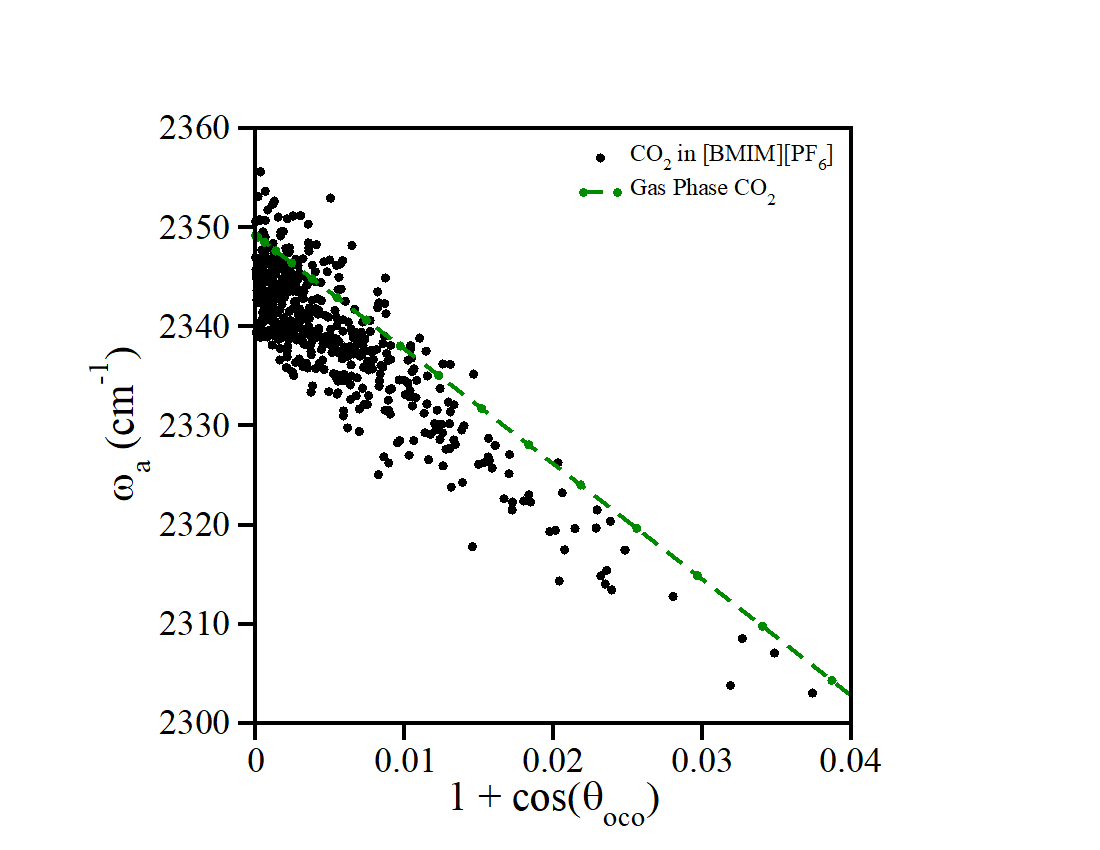
\includegraphics{paper_03/figure1.png}
  \caption{Relationship between the \ce{CO2} asymmetric stretch vibrational frequency and the \ce{OCO} angle, \(\theta_{\ce{OCO}}\), for \ce{CO2} in the gas-phase (green circles) and in the \ce{[C4C1im][PF6]} IL (black circles). The gas-phase data are perfectly correlated with \(1 + cos(\theta_{\ce{OCO}})\). The vibrational frequencies for \ce{CO2} in the \ce{[C4C1im][PF6]} solvent also show this relationship, but additional solvation effects on the frequency are also present.}
  \label{paper_03:fig1}
\end{figure}

\begin{figure}[H]
  \centering
  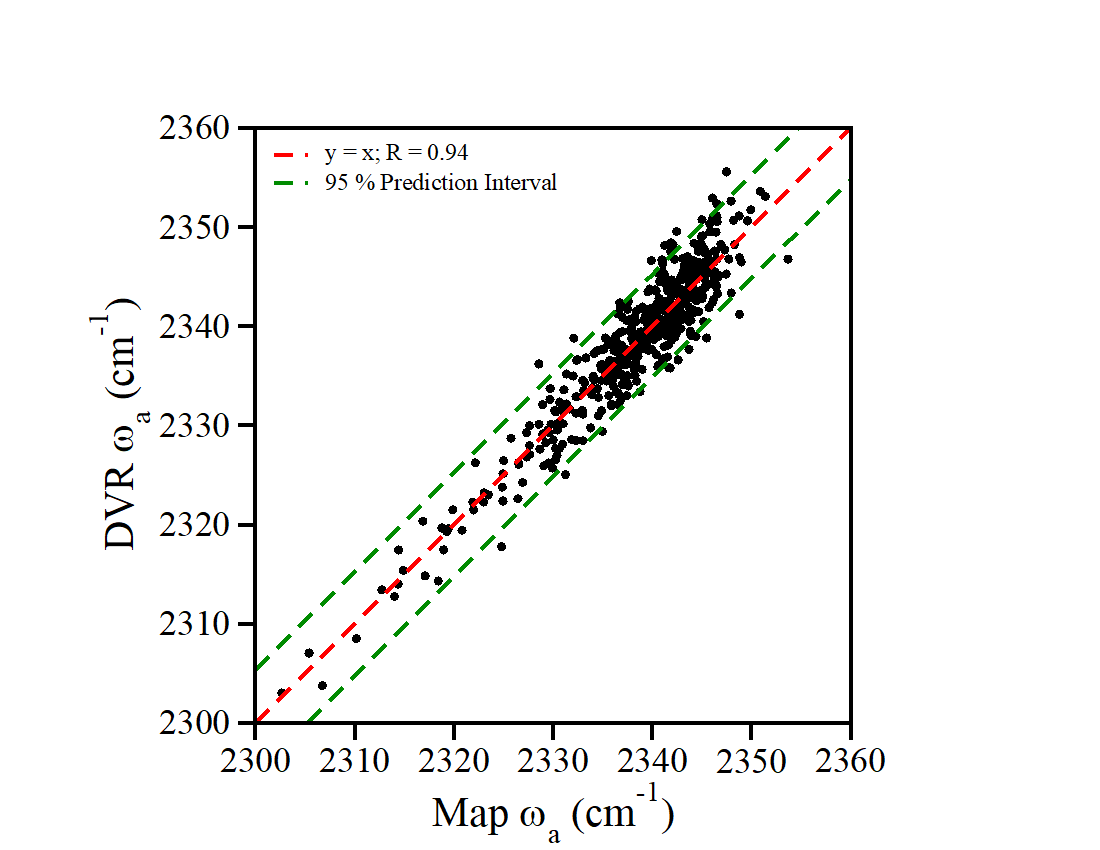
\includegraphics{paper_03/figure2.png}
  \caption[Spectroscopic map comparison with DVR]{Relationship between \ce{CO2} asymmetric stretch frequencies in the \ce{[C4C1im][PF6]} IL calculated using the DVR method and those calculated using the spectroscopic map for the 500 test set clusters (black circles). The red line represents a perfect correlation and the 95\% prediction interval is indicated with green lines. The spectroscopic map has a regression coefficient of \(R = 0.94\) and a root means squared error of \SI{2.7}{\wavenumber}.}
  \label{paper_03:fig2}
\end{figure}

\begin{figure}[H]
  \centering
  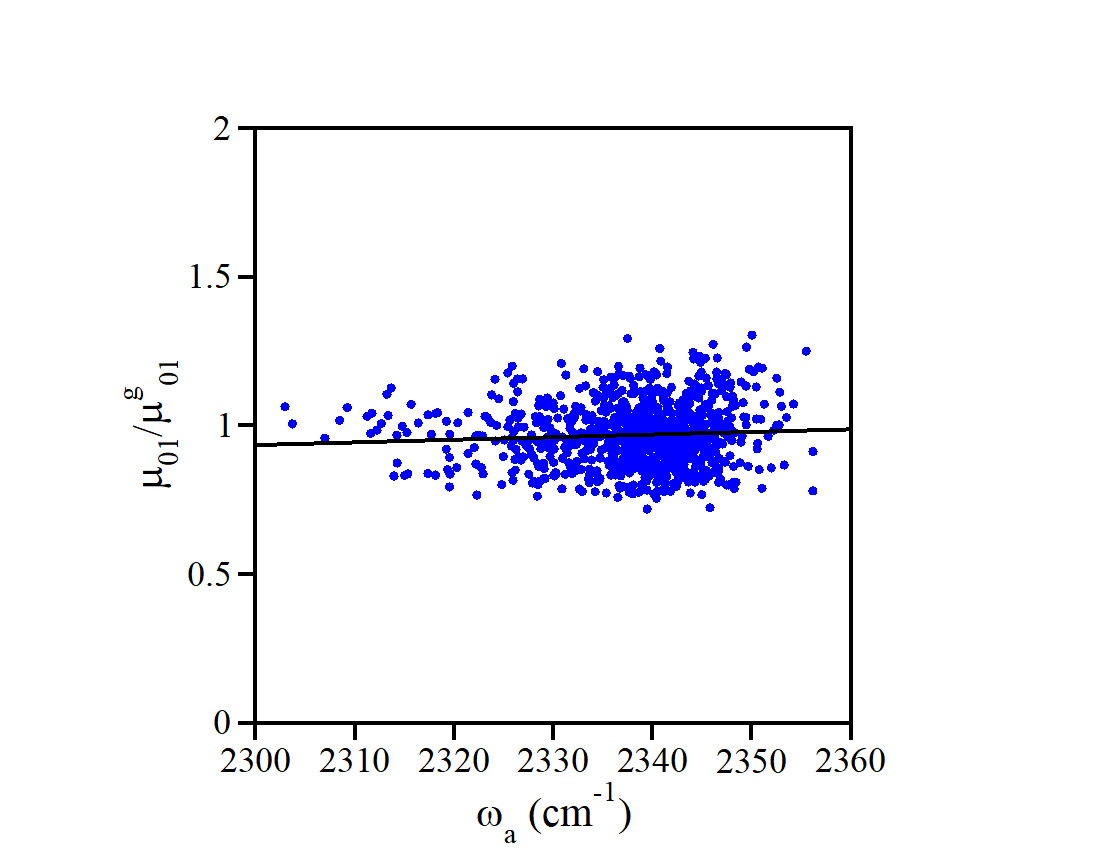
\includegraphics{paper_03/figure3.png}
  \caption{Transition dipole moment integral, \(\mu_{01}\), of the asymmetric stretch of \ce{CO2} in 1000 \ce{CO2}-\ce{[C4C1im][PF6]} clusters versus the asymmetric stretch vibrational frequency, \(\omega_{a}\), where \(\mu_{01}^{g}\) is the transition dipole moment integral of the asymmetric stretch of \ce{CO2} in the gas-phase (blue circles). A linear fit of the data (black line) has a slope close to zero indicating that the Condon approximation is reasonable for the asymmetric stretch of \ce{CO2} in the \ce{[C4C1im][PF6]} IL.}
  \label{paper_03:fig3}
\end{figure}

\begin{figure}[H]
  \centering
  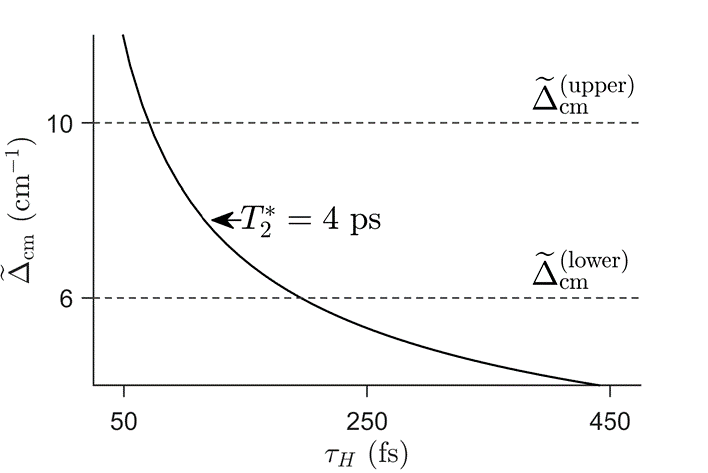
\includegraphics{paper_03/figure4.png}
  \caption[Linewidth dependence on correlation time for fast motions]{Homogeneous instantaneous linewidth as a function of correlation time for fast motions, with \(T_{2}^{*} = \SI{4}{\pico\second}\), with upper and lower bounds estimated for \({\widetilde{\Delta}}_{H}\). The upper bound, based on an estimated fastest allowed inertial response timescale, and the lower bound, based on a threshold value of \(\Delta_{H}\tau_{H}\), are indicated by dashed horizontal lines. The resulting instantaneous frequency range for homogeneous motions is between \SIrange{6}{10}{\wavenumber}.}
  \label{paper_03:fig4}
\end{figure}

\begin{figure}[H]
  \centering
  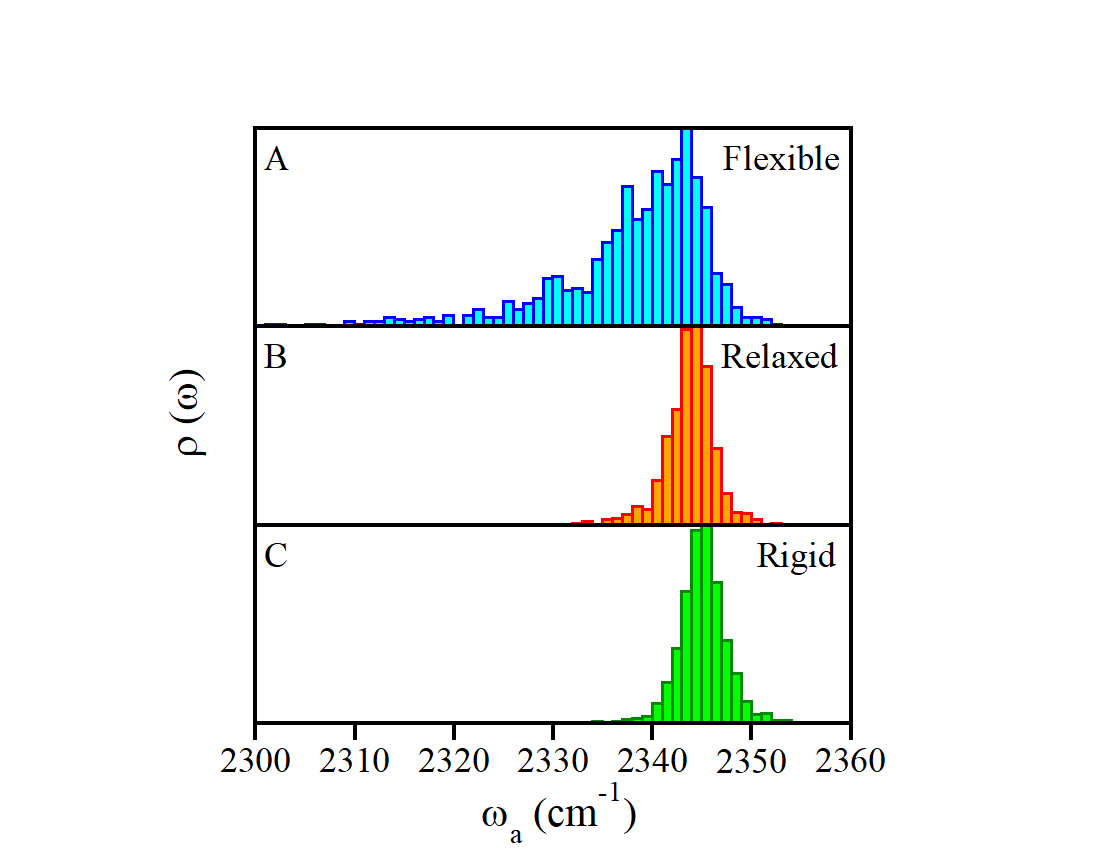
\includegraphics{paper_03/figure5.png}
  \caption{Histograms of the \ce{CO2} asymmetric stretch vibrational frequency, \(\omega_{a}\), for \num{1000} \ce{CO2}-\ce{[C4C1im][PF6]} clusters. (a) Clusters extracted from an MD simulation of flexible \ce{CO2} in the \ce{[C4C1im][PF6]} IL. (b) Clusters extracted from an MD simulation of flexible \ce{CO2} in the \ce{[C4C1im][PF6]} IL, but where the \ce{CO2} geometry is relaxed. (c) Clusters extracted from an MD simulation of rigid \ce{CO2} in the \ce{[C4C1im][PF6]} IL.}
  \label{paper_03:fig5}
\end{figure}

\section{\texorpdfstring{\caps{Supporting Information}}{Supporting Information}}
\label{paper_03:sec:SI}

Details regarding the transition dipole moment integral calculations in Figure~\ref{paper_03:fig3}.

\subsection{Transition Dipole Moment Calculations}

The intensity of a vibrational transition, \(\tilde{\nu}_{if}\), is related to the dipole moment matrix element between the two states, \(\Braket{\vec{\mu}_{if}}\)

\begin{equation}
  \label{paper_03:eq:S1}
  I \left( \tilde{\nu}_{if} \right) = \frac{8\pi^{3}N_{A}}{3hc\left( 4\pi\epsilon_{0} \right)} \tilde{\nu}_{if} \left| \vec{\mu}_{if} \right|^{2} (N_{i} - N_{f})
\end{equation}

where \(N_{A}\) is Avogadro's number, \(N_{k}\) is the number of particles in the \(k\)th state and \(\left| \vec{\mu}_{if} \right|^{2}\) is the squared norm of the transition dipole moment (TDM) integral between the two states.\cite{Carbonniere2010} Because all values in equation~\ref{paper_03:eq:S1} are constant (at a specific temperature) vibrational intensities for particular transitions are proportional to the squared norm of the TDM vector. Thus, the central property to calculate in order to evaluate the strength of the Condon approximation is \(\Braket{\vec{\mu}_{if}}\).

We can calculate the matrix elements of the dipole moment operator in a similar fashion as the bond length matrix elements were calculated in paper 1. Before, we used the value of the bond length at each grid point as a representation of the bond length operator. Similarly, we use the \(x\), \(y\), and \(z\) components of the dipole moment at each grid point (reported by a quantum chemistry program \textemdash{} in this case, Q-Chem\cite{Shao2015} \textemdash{} as the appropriate integral over the entire charge density) as a representation of the dipole moment operator,

\begin{equation}
  \label{paper_03:eq:S2}
  \vec{\mu} = \sum_{k = 1}^{3} \mu^k \widehat{k}
\end{equation}

where \(\widehat{k}\) is the \(k^{\text{th}}\) Cartesian basis vector. The dipole moment matrix elements are, for a two dimensional grid,

\begin{equation}
  \label{paper_03:eq:S3}
  \Braket{ \vec{\mu}_{if} } = \sum_{k = 1}^{3} \sum_{l = 1}^{N} \sum_{j = 1}^{N} \psi_{jl}^{i} \mu_{jl}^{k} \widehat{k} \psi_{jl}^{f}
\end{equation}

where the \(\psi_{jl}^{n}\) are the vibrational wavefunctions for state \(n\) on grid point \((j,l)\) returned by the DVR method. We have evaluated the accuracy of this method for \ce{CO2} in two ways. First, we calculate the norm of the TDM integral for the symmetric and asymmetric stretches of \ce{CO2} in the gas phase and compare these to experiment.\cite{DOWNING197566} The results are shown in Table~\ref{paper_03:tab:S1}, and the accuracy is excellent.

Next, we evaluated the accuracy of this method for \ce{CO2} in solution. A previously used method for evaluating the Condon approximation for vibrational reporters in solution is to (1) optimize the vibrational subsystem of interest with DFT while freezing all other degrees of freedom, (2) calculate the harmonic vibrational frequency and intensity for the vibrational subsystem using the same DFT method, then (3) repeat this for many statistically independent snapshots of the reporter in solution.\cite{schmidt_pronounced_2005-1} This process was completed for \num{25} snapshots of \ce{CO2} in IL solution for the asymmetric stretch. DVR asymmetric stretch frequencies and TDMs were also calculated for the \num{25} optimized (post step 1) snapshots. In order to facilitate comparison, the square roots of the intensities were taken. The resulting values and the TDMs were divided by their respective gas phase values. These values are plotted against each other in figure~\ref{paper_03:fig:S1}. The agreement between the two methods is excellent (\(R = 0.994\)). This new method has the advantage of being essentially computationally free to perform anytime a DVR calculation has already been done. Due to the possibility of parallelization, DVR calculations can be much more computationally inexpensive than regular vibrational frequency calculations.

\begin{table}[H]
  \centering
  \caption{Transition dipole moments for gas phase stretching modes of \ce{CO2}.}
  \label{paper_03:tab:S1}
  \begin{longtable}[]{@{}ccc@{}}
    \toprule
    Mode & DVR (\si{\debye}) & Experiment (\si{\debye})\cite{DOWNING197566}\tabularnewline
    \midrule
    \endhead
    \(\omega_{s}\) & \num{1.1e-13} & \num{0.0} \tabularnewline
    \(\omega_{a}\) & \num{3.4e-1} & \num{3.3e-1} \tabularnewline
    \bottomrule
  \end{longtable}
\end{table}

\begin{figure}[H]
  \centering
  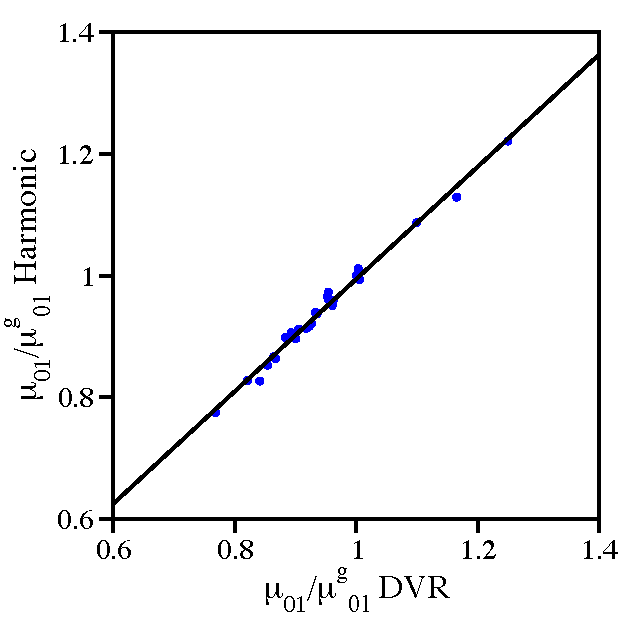
\includegraphics{paper_03/figureS1.pdf}
  \caption{Normalized transition dipole moment for the asymmetric stretch of \ce{CO2} as calculated by a quantum chemistry program and as calculated by the DVR method (blue dots). The black line is the best fit line, \(y = 0.97x + 0.07\). The correlation coefficient is 0.994.}
  \label{paper_03:fig:S1}
\end{figure}

\chapter[ALMO Linear Response]{A First Principles Approach for Partitioning Linear Response Properties into Additive and Cooperative Contributions}
\label{ch:paper_04}

The text in this chapter has been adapted from \fullcite{Berquist2018}. The author's contribution to the work included deriving the equations, implementing the algorithm, performing all calculations, and writing the manuscript.

\newcommand{\arlidimer}{\ce{Ar\bond{....}Li+}}

\newcommand{\aud}{\si{\bohr\cubed}}
\newcommand{\geomdeftsvp}{\SI{2.4106}{\angstrom}}
\newcommand{\geomdeftsvpd}{\SI{2.4297}{\angstrom}}

\newcommand{\pdalton}{\textsc{Dalton}}
\newcommand{\libresponse}{\texttt{libresponse}}
\newcommand{\psif}{\textsc{Psi4}}
\newcommand{\qchem}{\textsc{Q-Chem}}
\newcommand{\response}{\textsc{Response}}
\newcommand{\op}[1]{\ensuremath{\hat{#1}}}
\newcommand{\mat}[1]{\ensuremath{\mathbf{#1}}}
\newcommand{\Order}[1]{\ensuremath{\mathcal{O}\left(#1\right)}}
\newcommand{\tr}[1]{\ensuremath{{\mathrm{Tr}}\left\{#1\right\}}}
\newcommand{\eq}[1]{eq.~(\ref{#1})}
\newcommand{\citen}[1]{ref.~\parencite{#1}}
\newcommand{\lr}[2]{\braket{\braket{\op{#1}; \op{#2}}}}
\newcommand{\lrs}[4]{\braket{\braket{\op{#1}_{#2}; \op{#3}_{#4}}}}

\section{\texorpdfstring{\caps{Summary}}{Summary}}

We present the analytic implementation of linear response equations on top of absolutely localized molecular orbitals (ALMOs) as part of \libresponse{}, a library for solving the non-orthogonal molecular response equations for arbitrary operators. In the spirit of the original SCF(MI) and TDDFT(MI) formulations, our method is called linear response for molecular interactions, or LR(MI). Charge transfer was discovered to play an equally significant role in both the ground-state and response iterations.

\section{\texorpdfstring{\caps{Introduction}}{Introduction}}
\label{sec:introduction}

Experimental spectroscopy is a powerful tool for understanding the structure and function of molecular systems, especially when combined with theory and computation\cite{AUTSCHBACH200383,NEESE2009526,doi:10.1021/cr2002239}. Absolutely localized molecular orbitals (ALMOs)\cite{Khaliullin2006} and their associated energy decomposition analysis (ALMO-EDA)\cite{Khaliullin2007} provide a intuitive picture of how interactions at the microscopic scale translate to physical insight at the macroscopic scale. ALMO-EDA is capable of separating the total interaction energy of two or more user-defined arbitrary fragments into the following components:

\begin{equation}
  \label{eq:almo-eda}
  \Delta E_{\text{int}} = \Delta E_{\text{gd}} + \Delta E_{\text{frz}} + \Delta E_{\text{pol}} + \Delta E_{\text{CT}},
\end{equation}

where

\begin{itemize}
\item \(\Delta E_{\text{gd}}\) is the energy raising due to the distortion from each fragment's isolated geometry into the cluster geometry;
\item \(\Delta E_{\text{frz}}\) is the ``frozen density'' interaction, which accounts for classical electrostatics and Pauli repulsion between the fragments, and is usually positive;
\item \(\Delta E_{\text{pol}}\) is the polarization energy, which is the self-consistent response of each fragment's electron density in the field of the other fragments, and is always negative;
\item \(\Delta E_{\text{CT}}\) is the charge transfer interaction/energy, and is always negative.
\end{itemize}

This separation is achieved via a constrained self-consistent field calculation, called SCF for molecular interactions (SCF(MI)), producing ALMOs that incorporate fragment polarization but not charge transfer. There are multiple approximations to \(\Delta E_{\text{CT}}\), which can be further broken apart into a perturbative correction and higher-order effects stemming from a self-consistent treatment, where all orbital constraints are lifted and supersystem SCF iterations are performed (equation 5 in \citen{Khaliullin2008}):

\begin{equation}
  \label{eq:almo-eda-ct}
  \Delta E_{\text{CT}} = \Delta E_{\text{CT}}^{\text{RS}} + \Delta E_{\text{CT}}^{\text{HO}}.
\end{equation}

Each of these terms can be broken apart further into a sum of a true electron delocalization term and a BSSE term:

\begin{equation}
  \begin{aligned}
    \label{eq:almo-eda-ct-bsse}
    \Delta E_{\text{CT}}^{\text{RS}} &= \Delta E_{\text{del}}^{\text{RS}} + \Delta E_{\text{BSSE}}^{\text{RS}}, \\
    \Delta E_{\text{CT}}^{\text{HO}} &= \Delta E_{\text{del}}^{\text{HO}} + \Delta E_{\text{BSSE}}^{\text{HO}}.
  \end{aligned}
\end{equation}

Such an energy decomposition is made possible due to the bottom-up construction of ALMOs, where each ALMO is formed from atomic orbitals (AOs) only on a specific fragment, leading to MOs that are spatially localized onto fragments. In a previous work\cite{Brinzer_2015_212425}, we showed that a similar decomposition is possible for peaks in vibrational spectra according to

\begin{equation}
  \begin{aligned}
    \label{eq:almo-frequencies}
    \omega_{\text{tot}} &= \omega_{\text{free}} + \Delta \omega_{\text{int}}, \\
    \Delta \omega_{\text{int}} &= \Delta \omega_{\text{gd}} + \Delta \omega_{\text{frz}} + \Delta \omega_{\text{pol}} + \Delta \omega_{\text{CT}},
  \end{aligned}
\end{equation}

where each term has an analogous meaning to the original ALMO-EDA, except changes in the vibrational frequencies \(\{\omega\}\) rather than the interaction energy are used. We seek a more general decomposition of response properties, starting with those based on linear response (LR), where each \(\omega\) in \eq{eq:almo-frequencies} is replaced with \(\lr{P}{Q}_{\omega_{Q}}\), representing the influence of a perturbation \(\op{Q}\) with frequency \(\omega_{Q}\) on \(\op{P}\).

This is not the first work to seek a fragment- or subsystem-based decomposition of molecular response properties. The LoProp method\cite{doi:10.1063/1.1778131,JCC:JCC20632} starts from canonical orbitals and performs a series of localizations followed by orthogonalizations, leading to atom- and atom pair-centered contributions. While a top-down approach with only post-SCF localization avoids difficulties with a localized SCF implementation, the use of localized charges and dipole moments requires a finite difference approach beyond first derivatives. Several bottom-up approaches, where localized orbitals or subsystems are formed during the SCF iterations, also exist. More closely related to a many-body expansion (MBE) is the fragment molecular orbital (FMO)\cite{MOCHIZUKI2006418} calculation of frequency-dependent polarizabilities. The use of MBE-derived expressions requires a response calculation for each term in the fragment expansion, where ALMO-based LR solves the equations for all fragments simultaneously. Response equations have also been formulated within subsystem density functional theory (sDFT)\cite{Neugebauer_2009_84104,Pavanello_2013_204118}. sDFT requires the use of an additional kinetic energy functional, while ALMO-based LR can be used with all common exchange-correlation functionals. A comprehensive adaptation of response equations up to dynamic first and second hyperpolarizabilities\cite{JCC:JCC540120409} has been performed with nonorthogonal localized molecular orbitals (NOLMOs)\cite{doi:10.1021/acs.jctc.7b00321}. NOLMOs are not connected to an EDA, preventing a property decomposition into EDA-like terms that are the foundation of ALMO-based LR. An attractive fragment-based method designed specifically for the decomposition of molecular interaction energies is symmetry-adapted perturbation theory (SAPT)\cite{doi:10.1021/cr00031a008}, which is systematically improvable due to its foundations in perturbation theory. However, because the fragment orbitals are not variationally optimized together (unlike \(\Delta E_{\text{pol}}^{\text{ALMO-EDA}}\)), the formulation of derivatives even at the uncorrelated monomer approximation (SAPT0) is nontrivial.

The most related methods are those also built on top of ALMOs, specifically ALMO-CIS\cite{Closser_2015_5791}, ALMO-CIS+CT\cite{Ge_2017_44111}, TDDFT(MI)\cite{doi:10.1063/1.4926837}, and LEA-TDDFT\cite{doi:10.1021/acs.jctc.5b00828}. Compared to ALMO-CIS, our method is more consistent with the index restrictions in TDDFT(MI), and similarly to LEA-TDDFT, we can select individual fragments for allowing charge transfer. For this reason, our method is termed linear response for molecular interactions, or LR(MI).

To this end, we have developed \libresponse{}, a molecular response library for non-orthogonal orbitals and arbitrary operators, in the spirit of the \response{} module of \pdalton{}\cite{daltonpaper}. It is capable of both singlet\cite{doi:10.1063/1.454885} and triplet\cite{doi:10.1063/1.457471} response for restricted and unrestricted wavefunctions using Hartree-Fock (HF) or density functional theory (DFT). Properties can be calculated using either the full time-dependent Hartree-Fock (TDHF) or random phase approximation (RPA) equations, or with the configuration interaction with singles (CIS) approximation\cite{doi:10.1021/j100180a030}. Our current implementation is limited to linear response and static properties (\(\omega = 0\)), with both non-linear response and dynamic properties under current development.

\section{\texorpdfstring{\caps{Theory}}{Theory}}
\label{sec:theory}

For the remainder of the paper, unless otherwise stated, the indices \(i,j,k,l,...\) correspond to unoccupied MOs, \(a,b,c,d,...\) correspond to virtual/unoccupied MOs, \(\mu,\nu,\lambda,\sigma,...\) correspond to AOs, and \(I,J,...\) correspond to fragments. There is no distinction between canonical MO and ALMO indices. Comma-separated indices such as \(ia,jb\) correspond to a matrix with a compound index \(ia\) and another compound index \(jb\).

\subsection{Linear response formalism}
\label{ssec:linear-response-formalism}

The linear response of a molecule in its ground state \(\ket{0}\) to perturbations corresponding to operators \(\op{P}\) and \(\op{Q}\) can be written as the sum over all excited states \(\{n\}\),

\begin{equation}
  \lr{P}{Q}_{\omega}
  =
  - \sum_{n > 0} \;
    \left[
      \frac{\braket{0|\op{P}|n} \braket{n|\op{Q}|0}}{\omega_{n} - \omega}
    + \frac{\braket{0|\op{Q}|n} \braket{n|\op{P}|0}}{\omega_{n} + \omega}
    \right],
\end{equation}

where \(\omega\) is the frequency of the perturbation \(\op{Q}\) and \(\omega_{n} = E_{n} - E_{0}\). Examples of second-order response properties include the polarizability (\(\op{P} = \op{Q} = \op{\mu}\)), magnetizability (\(\op{P} = \op{Q} = \op{m}\)), vibrational frequencies (\(\op{P} = \op{Q} = \op{x}\)), etc. This paper focuses on molecular response within the static limit (\(\omega = 0\)),

\begin{equation}
  \lr{P}{Q}_{0}
  =
  - \tr{\mat{P}^{\dagger} \mat{G}^{-1} \mat{Q}}
  =
  - \tr{\mat{P}^{\dagger} \mat{X}},
\end{equation}

where \((\mat{P})_{ia} = \braket{i|\op{P}|a}\) and \((\mat{Q})_{ia} = \braket{i|\op{Q}|a}\). \(\mat{X} = \mat{G}^{-1} \mat{Q}\) is the ``response vector'' corresponding to orbital rotations induced by perturbation \(\op{Q}\). The orbital Hessian matrix \(\mat{G}\) is defined as

\begin{equation}
  \begin{aligned}
    ^{RR}\mat{G}^{\sigma} &= \mat{A}^{\sigma} + \mat{B}^{\sigma} \\
    ^{II}\mat{G}^{\sigma} &= \mat{A}^{\sigma} - \mat{B}^{\sigma}
  \end{aligned}
\end{equation}
for real (\(R\)) and imaginary (\(I\)) perturbations, respectively\cite{doi:10.1080/00268976.2015.1024182}. The spin case \(\sigma\) can either be singlet (\(\sigma = s\)) or triplet (\(\sigma = t\)) depending on whether the perturbation operator conserves or flips spin, respectively:

\begin{equation}
  \begin{aligned}
    A^{s}_{ia,jb} &= \Delta_{ia} + 2(ia|jb) - (ij|ab) \\
    A^{t}_{ia,jb} &= \Delta_{ia} - (ij|ab)
  \end{aligned}
\end{equation}

\begin{equation}
  \begin{aligned}
    B^{s}_{ia,jb} &= 2(ia|jb) - (ib|ja) \\
    B^{t}_{ia,jb} &= - (ib|ja)
  \end{aligned}
\end{equation}

where \(\Delta_{ia} = (\varepsilon_{a} - \varepsilon_{i}) \delta_{ia,jb}\) is an orbital energy difference. The CIS or Tamm-Dancoff approximation (TDA) is recovered when \(\mat{B} = \mat{0}\). Rather than directly inverting the orbital Hessian, which would cost \Order{o^3 v^3}, one solves iteratively for \(\mat{X}\) by expanding the inverse, for example in the real singlet case

\begin{equation}
  \label{eq:update}
  X_{ia}^{(n+1)}
  =
  \frac{Q_{ia} - \left[4(ia|jb) - (ij|ab) - (ib|ja)\right] X_{jb}^{(n)}}
       {\Delta_{ia}}
\end{equation}

Repeated indices imply summation (Einstein sum convention). Here, the superscript in parentheses denotes the iteration number. To avoid the expensive transformation of two-electron repulsion integrals from atomic orbital into molecular orbital basis, one performs the contraction over orbital pair \(jb\) in the atomic orbital basis,

\begin{equation}
  \left(\mat{A}^{s} + \mat{B}^{s}\right)_{ia,jb} X_{jb}
  =
  C_{\mu i}
  \left[
    4 (\mu\nu|\lambda\sigma) D_{\lambda\sigma}^{X}
    - (\mu\lambda|\nu\sigma) D_{\lambda\sigma}^{X}
    - (\mu\sigma|\lambda\nu) D_{\lambda\sigma}^{X}
  \right]
  C_{\nu a}
\end{equation}

with the perturbed density matrix \(D_{\mu\nu}^{X} = C_{\lambda j} X_{jb} C_{\sigma b}\).

To work with \emph{non-orthogonal orbitals}, we replace the \(\Delta_{ia}^{-1}\) denominator in \eq{eq:update} with a full matrix inversion of

\begin{equation}
  \label{eq:energy-denominator}
  E_{ia,jb} = F_{ab}S_{ij} - F_{ij}S_{ab},
\end{equation}

where \(\mat{F}\) and \(\mat{S}\) are the MO-basis Fock and overlap matrix, respectively

\subsection{Adaptation of linear response equations for absolutely localized MOs}
\label{ssec:almo-adaptation}

The first requirement for adapting the non-orthogonal linear response equations to the ALMO formalism is the projection of the occupied subspace from the virtual subspace. This is because the original fragment-local virtual ALMOs are not orthogonal to occupied ALMOs on other fragments. We form ``modified'' or ``projected'' virtual orbitals,

\begin{equation}
  \label{eq:projected-virtuals}
  \ket{\phi_{a}} = N_{a} \left( 1 - \op{D}_{\text{occ}} \right) \ket{\psi_{a}}
\end{equation}

where \(\op{D}_{\text{occ}} \rightarrow (\mat{D}_{\text{occ}})_{\mu\nu} = C_{\mu i} C_{\nu i}\). Otherwise, this contamination would manifest as spurious low-lying excited states, leading to artificial poles in the polarizability. This requirement for projection is unimportant for ground-state SCF(MI) calculations, where the virtual orbitals do not have an effect on the final result (energy).

The second requirement is to maintain consistency with the fragment-local nature of SCF(MI), where CT is not allowed. Each occupied-virtual MO contribution to the molecular response is restricted to be within the same fragment. This corresponds to forcing all \(ia\) (or \(jb\)) pairs to be zero when \(i \in F_{I}, a \in (F_{J} \neq F_{I})\). Algorithmically, we do this by always working in the full CT-allowed basis, then zeroing out CT-disallowed matrix elements. For the energy denominator, the zero rows and columns must be removed to avoid introducing artificial singularities. The advantage of working in the full CT basis and zeroing matrix elements is twofold: it prevents code duplication due to no need for separate non-orthogonal and ALMO-based response routines, and it enables selection of individual fragments to quantify their CT contribution to the final response property. This is in contrast to ALMO-CIS+CT\cite{Ge_2017_44111}, which starts from the reduced CT-disallowed basis and adds a distance-dependent CT correction. An outline of the algorithm is available in the SI.

Perhaps the most important fundamental distinction between our formulation of the ALMO response equations and the ALMO-CIS formulation is in the two-electron contribution, where we restrict MO indices but do not restrict AO indices. This means that for a given \(J_{\mu\nu}^{X} = (\mu\nu|\lambda\sigma)D_{\lambda\sigma}^{X}\), summations run over AO indices on all fragments, and both \((\mu\nu|\lambda\sigma)\) and \(D_{\lambda\sigma}^{X}\) for \(\lambda\in F_{I}, \sigma\in (F_{J} \neq F_{I})\) may be non-zero. Additionally, AO indices cannot be restricted due to the projection in \eq{eq:projected-virtuals}, where each MO can have contributions from all AOs.

In principle, the ALMO formulation presented here can be extended to arbitrary-order response, as long as each compound \(ia\) index is constrained to be within a fragment.

\subsection{Decomposition of linear response properties into local contributions and interaction mechanisms}
\label{ssec:decomp-line-resp}

As with other localized orbital schemes, there is a question of how to define charge transfer. Our implementation allows for the introduction of CT in several stages. This allows for further decomposition of the CT term into qualitative contributions from individual fragments. This is done by starting from the polarized SCF(MI) wavefunction and allowing transitions between the occupied space of a single fragment into the virtual space of all fragments. This can be denoted as ``frz + pol + CT(\(F \rightarrow\) all)'', where \(F\) is an individual fragment. The difference between this result and ``frz + pol'' can be viewed as how important CT is for that specific fragment \(F\). From the symmetry-adapted perturbation theory\cite{STONE2009201} perspective, it can also be viewed as a BSSE correction; the larger the difference, the more deficient the fragment-localized basis is. CT can also be allowed during the response calculation even if it was not during the wavefunction calculation; this corresponds to performing non-orthogonal response with no restrictions using the polarized SCF(MI) wavefunction, represented as ``frz + pol + CT(all \(\rightarrow\) all) [blocked]''. The sum over all fragments should be qualitatively equal to ``frz + pol + CT(all \(\rightarrow\) all) [blocked]'', though it will not be exactly equal due to higher-order effects, similar to the \(\Delta E_{\text{CT}}^{\text{HO}}\) term in ALMO-EDA. Finally, ``frz + pol + CT(all \(\rightarrow\) all) [blocked]'' corresponds to an unrestricted response calculation on top of the fully-relaxed SCF wavefunction, analogous to a supersystem calculation. The difference between the blocked result and the supersystem result shows the effect of allowing CT in the underlying wavefunction.

This multi-step decomposition of the CT term is similar to our previous work on the effect of CT on the vibrational spectra of \ce{CO2} in ionic liquids\cite{Brinzer_2015_212425,Berquist_2017_208}. Being able to turn CT on and off during the geometry optimization and numerical Hessian calculation allowed us to see how CT contributes to the potential energy surface at multiple stages, but our analytic formulation of the response equations has significant advantages. It enables the identification of fragment-specific contributions to the total response, which is not possible in a numerical response calculation, even with an underlying SCF(MI) wavefunction. This is in addition to all the other advantages of solving analytic rather than numerical equations, namely calculation time, uncoupled and perturbative approximations to fully iterative results, lack of finite-difference error, frequency-dependent perturbations, and response to applied magnetic fields without complex energies; see \citen{gauss2000} for a discussion.

Borrowing terminology from \citen{Berquist_2017_208}, CT may enter the response calculation through multiple mechanisms. We consider two: the ``wavefunction mechanism'', where CT is (dis)allowed during the SCF iterations, corresponding to either an SCF(MI) or a canonical SCF calculation, and the ``response mechanism'', where CT is (dis)allowed during the response calculation by restricting occupied-virtual MO contributions to be within fragments as discussed in section~\ref{ssec:almo-adaptation}. This results in four principal permutations of (dis)allowing CT effects, abbreviated as ``\(a/b\)'', where \(a\) represents the wavefunction mechanism, \(b\) represents the response mechanism, and \(a,b\in\{\text{on},\text{off}\}\):

\begin{itemize}
\item ``on/on'' is a standard response calculation, and is the ``frz + pol + CT(all \(\rightarrow\) all) [super]'' result.
\item ``off/off'' is the most consistent with SCF(MI) and TDDFT(MI), and is the ``frz + pol'' result.
\item ``off/on'' attempts to recover CT effects during the response calculation that are missing from the underlying SCF(MI) wavefunction, and is the ``frz + pol + CT(all \(\rightarrow\) all) [blocked]'' result. This is not the same as the single perturbative Roothaan step (RS) correction in SCF(MI), but is a fully-iterative response calculation on top of ALMOs.
\item ``on/off'' corresponds to allowing CT during SCF iterations but not the response calculations. This decomposition is not considered, as neither the occupied nor the virtual canonical orbitals can generally be assigned to specific fragments.
\end{itemize}

For the purposes of this work, we also do not consider the effect of disallowing CT during geometry optimization through the ``geometry mechanism'', though in principle it is technically feasible and potentially non-negligible. See \citen{Mao_2017_5944} for an in-depth analysis of the different potential energy surfaces that comprise ALMO-EDA. Neglecting the geometry mechanism means our approach is consistent with a vertical decomposition rather than an adiabatic one.

\section{\texorpdfstring{\caps{Methods}}{Methods}}
\label{sec:methods}

HF was used for all calculations as a proof of concept to avoid spurious overdelocalization and CT effects due to self-interaction error. As a result, it should provide a lower bound on any possible CT effects during the SCF(MI) calculation. For basis sets, we chose the Karlsruhe def2- family\cite{Weigend_2005_3297,Rappoport_2010_134105}, in particular def2-SVP and def2-SVPD. It is well-known that the original ALMO procedure has a strong basis-set dependence, with overestimation of \(\Delta E_{\text{pol}}\) and underestimation of \(\Delta E_{\text{CT}}\) due to the overlapping tails of AOs on different fragments, allowing electron density to ``leak'' across fragments during SCF(MI)\cite{doi:10.1063/1.4792434}. As a result, there is no clear basis set limit to \(\Delta E_{\text{pol}}\). This informs our basis set choices, which should give qualitatively correct results within the original ALMO definition, with a check on minimal augmentation optimized for use in electric field response calculations.

For a test property, we chose the static dipole polarizability, defined as

\begin{equation}
  \alpha_{ab}(0) = -\lrs{\mu}{a}{\mu}{b}_{0} = -\left.\frac{\partial^{2} E}{\partial \varepsilon_a \partial \varepsilon_b}\right|_{\varepsilon_{a},\varepsilon_{b}=0},
\end{equation}

where \(a,b \in \{x,y,z\}\) and the energy derivative method based on derivatives with respect to applied electric fields \(\varepsilon\) is equivalent to the linear response calculation.

For a test system, the argon\textemdash{}lithium cation dimer, \arlidimer{}, was chosen due to the reasonable polarizability of the bare (closed-shell) argon atom, which should be quantitatively influenced by the almost unscreened nuclear charge of the lithium cation. The optimized distances are \geomdeftsvp{} using def2-SVP and \geomdeftsvpd{} using def2-SVPD. For the distance dependence results, points are spaced at \SI{0.05}{\angstrom} from \SIrange{1.25}{5.00}{\angstrom}, then spaced at \SI{0.25}{\angstrom} from \SIrange{5.00}{10.00}{\angstrom}.

All calculations were performed using a development version of \qchem{}\cite{Shao2015} compiled with \libresponse{}, our generalized non-orthogonal molecular response library. Thresholds were set to \num{e-14} for integral screening, \num{e-11} for the DIIS error norm in SCF convergence, and \num{e-8} for the DIIS error norm in the analytic response iterations. The Stoll projector equations were used for minimizing the underlying SCF(MI) wavefunction\cite{Stoll_1980_169,Khaliullin2006}. For numerical polarizability calculations, 2nd-order finite difference from energies was used, unless otherwise stated, as differences between 1st- and 2nd-order results were below \num{e-7} \aud{} in all cases. Both 1st- and 2nd-order finite difference polarizability calculations used a finite field step size of \num{1.88973e-5} \aud{}. All SCF(MI) analytic polarizability calculations use projected virtual orbitals as defined by \eq{eq:projected-virtuals}.

\section{\texorpdfstring{\caps{Results and Discussion}}{Results and Discussion}}
\label{sec:results-and-discussion}

\subsection{Equilibrium distance}
\label{ssec:results-equilibrium-distance}

\begin{table}
  \centering
  \caption[Argon\textemdash{}lithium cation dimer polarizabilities using HF/def2-SVP]{Polarizability results for the argon\textemdash{}lithium cation dimer at the HF/def2-SVP level. The geometry is optimized at the same level. All values have units of \aud{}.}
  \label{table:polarizability-results-def2-svp}
  \begin{tabular}{lrrrrrr}%
\toprule%
&\multicolumn{3}{c}{analytical}&\multicolumn{3}{c}{numerical}\\%
\cmidrule{2-4}\cmidrule{5-7}%
def2-SVP&\(\alpha_{\perp}\)&\(\alpha_{\parallel}\)&\(\alpha_{\text{iso}}\)&\(\alpha_{\perp}\)&\(\alpha_{\parallel}\)&\(\alpha_{\text{iso}}\)\\%
\midrule%
monomer A (\ce{Ar})&4.3702&4.3702&4.3702&4.3702&4.3702&4.3702\\%
monomer B (\ce{Li+})&0.1593&0.1593&0.1593&0.1593&0.1593&0.1593\\%
A + B&4.5295&4.5295&4.5295&4.5295&4.5295&4.5295\\%
frz + pol&4.5042&4.5581&4.5222&4.5036&4.5696&4.5256\\%
+ CT(A \(\rightarrow\) all)&4.7040&5.5191&4.9757&\textemdash{}&\textemdash{}&\textemdash{}\\%
+ CT(B \(\rightarrow\) all)&0.1594&0.1586&0.1591&\textemdash{}&\textemdash{}&\textemdash{}\\%
+ CT(all \(\rightarrow\) all) [blocked]&4.8409&5.7540&5.1452&\textemdash{}&\textemdash{}&\textemdash{}\\%
+ CT(all \(\rightarrow\) all) [super]&5.2142&7.8649&6.0978&5.2142&7.8649&6.0978\\%
\bottomrule%
\end{tabular}

\end{table}

\begin{table}
  \centering
  \caption[Argon\textemdash{}lithium cation dimer polarizabilities using HF/def2-SVPD]{Polarizability results for the argon\textemdash{}lithium cation dimer at the HF/def2-SVPD level. The geometry is optimized at the same level. All values have units of \aud{}.}
  \label{table:polarizability-results-def2-svpd}
  \begin{tabular}{l|rrr|rrr}%
\hline%
\hline%
\ce{Ar\bond{....}Li+}&\multicolumn{3}{c}{analytical}&\multicolumn{3}{c}{numerical}\\%
\hline%
def2-SVPD&\(\alpha_{\perp}\)&\(\alpha_{\parallel}\)&\(\alpha_{\text{iso}}\)&\(\alpha_{\perp}\)&\(\alpha_{\parallel}\)&\(\alpha_{\text{iso}}\)\\%
\hline%
monomer A (\ce{Ar})&10.3735&10.3735&10.3735&10.3735&10.3735&10.3735\\%
monomer B (\ce{Li+})&0.1603&0.1603&0.1603&0.1603&0.1603&0.1603\\%
A + B&10.5338&10.5338&10.5338&10.5338&10.5338&10.5338\\%
frz + pol&10.0787&10.6399&10.2658&10.0875&10.6599&10.2783\\%
frz + pol + CT(A \(\rightarrow\) all)&10.0157&10.4900&10.1738&{-}{-}&{-}{-}&{-}{-}\\%
frz + pol + CT(B \(\rightarrow\) all)&0.1606&0.1614&0.1609&{-}{-}&{-}{-}&{-}{-}\\%
frz + pol + CT(all \(\rightarrow\) all) [blocked]&10.1395&10.8004&10.3598&{-}{-}&{-}{-}&{-}{-}\\%
frz + pol + CT(all \(\rightarrow\) all) [super]&10.0724&11.0645&10.4031&10.0724&11.0645&10.4031\\%
\hline%
\hline%
\end{tabular}
\end{table}

Tables~\ref{table:polarizability-results-def2-svp}~and~\ref{table:polarizability-results-def2-svpd} show equilibrium distance results for the argon\textemdash{}lithium cation dimer at the HF/def2-SVP and HF/def2-SVPD levels, respectively. Due to molecular symmetry, two of the three polarizability tensor principal components are identical; these correspond to the perpendicular polarizability \(\alpha_{\perp}\), or how easy it is to shift the electron density perpendicular to the interatomic axis. The parallel polarizability \(\alpha_{\parallel}\) corresponds to the principal component that lies along the axis of interaction between the two atoms and corresponds to the bond polarizability. Monomer A and B refer to the isolated atoms; parallel and perpendicular axes have no meaning here due to their spherical symmetry, as all principal components are identical. An approximation to the frozen density interaction in response is the sum of the response of the isolated fragments (atoms), shown as ``A + B''. Note that this is not the true frozen monomer response\cite{Mao_2017_5944}. ``frz + pol'' is where CT is disallowed between fragments using the algorithm described above, consistent with the original SCF(MI) and conceptually analogous to TDDFT(MI). The remaining entries are those described in section~\ref{ssec:decomp-line-resp}.

\subsubsection{Validation of analytic ALMO results}
\label{sssec:results-validation}

As a correctness check, our analytic formulation is validated against finite-field calculations in the last three columns. An advantage of the analytic formulation is the ability to further decompose the CT term; it is not possible to perform the ``CT(A \(\rightarrow\) all)'', ``CT(B \(\rightarrow\) all)'', and ``CT(all \(\rightarrow\) all) [blocked]'' calculations with a finite-field approach. For both basis sets presented, there is no quantitative difference between the analytic and numerical polarizabilities except for ``frz + pol''. This should not be interpreted as an error, since our definition of the response equations differs from the no-CT formulation presented by ALMO-CIS, and there is a slight delocalization of the virtual space due to the projection (see section~\ref{sec:conclusions-and-future-work}). Still, the largest percent difference is 0.25\% and 0.19\% in \(\alpha_{\parallel}\) for def2-SVP and def2-SVPD, respectively, showing our definition should be valid as long as the ALMO approximation holds.

\subsubsection{CT mechanism analysis}
\label{sssec:ct-mechanism-analysis}

From tables~\ref{table:polarizability-results-def2-svp}~and~\ref{table:polarizability-results-def2-svpd}, the importance of charge transfer via both the wavefunction and response mechanisms can be calculated as the difference between ``frz + pol'', ``CT(all \(\rightarrow\) all) [blocked]'', and ``CT(all \(\rightarrow\) all) [super]''; these are ``off/off'', ``off/on'', and ``on/on'', respectively. The effect of each mechanism is shown in table~\ref{tab:mechanism-percentage-changes}.

\begin{table}
  \centering
  \caption[Percentage changes in argon\textemdash{}lithium cation dimer \(\alpha_{\parallel}\) due to the two CT mechanisms]{Percentage changes in \(\alpha_{\parallel}\) due to the two CT mechanisms. The reference (denominator) polarizability used is shown in \textit{italics}. All calculations used a bond length of \geomdeftsvpd{}.}
  \label{tab:mechanism-percentage-changes}
  \begin{tabular}{ccc}
    \toprule
                                           & \multicolumn{2}{c}{basis set} \\
    percentage change due to mechanism     & def2-SVP    & def2-SVPD       \\
    \midrule
    response (\textit{off/on} - off/off)   & 20.8        & 1.5             \\
    wavefunction (\textit{on/on} - off/on) & 26.8        & 2.4             \\
    \bottomrule
  \end{tabular}
\end{table}

For def2-SVP, it is clear that each successive relaxation of CT restrictions has a non-negligible effect on the final property, where \(\alpha_{\parallel}^{\text{frz + pol}}\) is 58.0\% and 96.2\% of the supermolecular value for the two basis sets. This representation makes it clear that in addition to larger polarizabilities (\(\sim 2 \times\)), there are other fundamental differences caused by the use of diffuse functions in def2-SVPD.

% Viewed another way, if CT does not contribute strongly to the interaction of fragments, a large fraction of the supermolecular or canonical SCF result should recovered regardless of the CT restriction level, in the spirit of the original SCF(MI) approximation\cite{Khaliullin2006}. These fractions are shown in table~\ref{tab:mechanism-percentage-of-super}

% \begin{table}
%   \begin{tabular}{ccc}
%     \toprule
%                                 & \multicolumn{2}{c}{basis set} \\
%     \fxnote{?}   & def2-SVP    & def2-SVPD   \\
%     \midrule
%     (off/off) / (off/on)        & 79.2        & 98.5            \\
%     (off/off) / (on/on)         & 58.0        & 96.2            \\
%     (off/on) / (on/on)          & 73.2        & 97.6            \\
%     \bottomrule
%   \end{tabular}
%   \caption{Percent contribution of each mechanism \fxnote{?}. All calculations used a bond length of \geomdeftsvpd{}.}
%   \label{tab:mechanism-percentage-of-super}
% \end{table}

Calculated this way, the wavefunction mechanism may include some higher-order effects, as the pure wavefunction mechanism, calculated as ``on/off'' - ``off/off'',  cannot be isolated due to the ``on/off'' term (see section~\ref{ssec:decomp-line-resp}). The size of these higher-order effects in the wavefunction can be estimated by the percent contribution of higher-order effects in ALMO-EDA charge transfer, shown in table~\ref{tab:almo-eda-higher-order-pct-of-ct}.

\begin{table}
  \centering
  \caption[Percentage of ALMO-EDA charge transfer in argon\textemdash{}lithium cation dimer due to higher-order effects]{Percentage of ALMO-EDA charge transfer due to higher-order effects, calculated as \(100 * \frac{\Delta E_{\text{CT}}^{\text{HO}}}{\Delta E_{\text{CT}}^{\text{RS}} + \Delta E_{\text{CT}}^{\text{HO}}}\). All calculations used a bond length of \geomdeftsvpd{}.}
  \label{tab:almo-eda-higher-order-pct-of-ct}
  \begin{tabular}{ccc}
    \toprule
                    & \multicolumn{2}{c}{basis set} \\
    BSSE corrected? & def2-SVP    & def2-SVPD   \\
    \midrule
    no              & 24.2        & 17.1        \\
    yes             & 25.0        & 19.4        \\
    \bottomrule
  \end{tabular}
\end{table}

Using the uncorrected results for consistency, the new estimates of percentage changes due to the wavefunction mechanism become 20.3\% and 2.0\%, showing the presence of CT in the underlying wavefunction and in the response calculation are equally important in predicting molecular properties.

\subsubsection{Basis set dependence}
\label{sssec:basis-set-dependence}

The results in table~\ref{tab:mechanism-percentage-changes} show that charge transfer, or electron delocalization across fragments, is relatively unimportant when using the diffuse basis set. This may be indicative of either basis set incompleteness or overlap between the tails of the diffuse basis functions (see section~\ref{sec:methods}). The former argument is supported by the BSSE term being 50\% of the total CT term with def2-SVP but only 18\% with def2-SVPD, while the latter argument is supported by a doubling of \(\Delta E_{\text{pol}}\) from \SIrange{-3.3}{-6.6}{\kcal\per\mol} when adding the diffuse functions (see the SI for all ALMO-EDA results).

To investigate these effects directly on the polarizability, rather than through an EDA, table~\ref{tab:basis-set-dependence} shows the decoupled effect of the nuclear charge and basis functions provided by the lithium cation on the argon. Since the lithium cation is not very polarizable (\(\alpha^{\ce{Li+}}\) is \(\approx 4\%\) of \(\alpha^{\ce{Ar}}\) at the HF/def2-SVP level), only effects on the argon atom are considered. Also presented are the lowest singlet and triplet excitation energies calculated using RPA (TD-HF). Percentages of each value compared to the full \arlidimer{} result within each basis set are shown in the SI.

In order to test the importance of nuclear charge without the influence of basis functions, the ``PC(+)'' and ``PC(-)'' entries represent replacing the lithium atom with positive and negative point charges of unit magnitude, respectively. To test the importance of the basis set without the influence of a nuclear charge, ``Gh(Li)'' represents replacing the full lithium atom with only its basis functions, leaving a ``ghost atom'' with no (effective) nuclear charge. This should separate the \arlidimer{} interaction into a purely electrostatic effect from the nucleus, a delocalization-like effect due to increased spatial flexibility for motion of electrons during SCF and response iterations, and some non-additive effects.

\begin{table}
  \centering
  \caption[Point charge and basis function contributions to argon\textemdash{}lithium cation dimer polarizabilities]{Decomposition of polarizabilities into point charge and basis function contributions. All calculations used canonical MOs and a distance of \geomdeftsvpd{} from argon to the other center(s).}
  \label{tab:basis-set-dependence}
  \begin{tabular}{llrrrrr}
\toprule
 basis set &                          structure & \(\alpha_{\perp}\) (a.u.) & \(\alpha_{\parallel}\) (a.u.) & \(\bar{\alpha}\) (a.u.) & \(^{\text{t}}E_{0 \rightarrow \text{lowest}}^{\text{RPA}}\) (eV) & \(^{\text{s}}E_{0 \rightarrow \text{lowest}}^{\text{RPA}}\) (eV) \\
\midrule
  def2-SVP &   \ce{Ar\bond{....}PC(\mathrm{-})} &                      4.38 &                          4.35 &                    4.37 &                                                            23.26 &                                                            25.09 \\
  def2-SVP &                            \ce{Ar} &                      4.37 &                          4.37 &                    4.37 &                                                            23.69 &                                                            25.50 \\
  def2-SVP &   \ce{Ar\bond{....}PC(\mathrm{+})} &                      4.36 &                          4.38 &                    4.37 &                                                            23.42 &                                                            25.24 \\
  def2-SVP &  \ce{Ar\bond{....}\mathrm{Gh}(Li)} &                      4.89 &                          6.23 &                    5.34 &                                                            12.26 &                                                            12.58 \\
  def2-SVP &              \ce{Ar\bond{....}Li+} &                      5.21 &                          7.88 &                    6.10 &                                                            11.90 &                                                            12.18 \\
 def2-SVPD &   \ce{Ar\bond{....}PC(\mathrm{-})} &                     10.94 &                         10.33 &                   10.74 &                                                            10.92 &                                                            11.68 \\
 def2-SVPD &                            \ce{Ar} &                     10.37 &                         10.37 &                   10.37 &                                                            12.61 &                                                            13.22 \\
 def2-SVPD &   \ce{Ar\bond{....}PC(\mathrm{+})} &                     10.04 &                         11.94 &                   10.67 &                                                             9.90 &                                                            10.48 \\
 def2-SVPD &  \ce{Ar\bond{....}\mathrm{Gh}(Li)} &                     10.39 &                         10.42 &                   10.40 &                                                            12.05 &                                                            12.41 \\
 def2-SVPD &              \ce{Ar\bond{....}Li+} &                     10.07 &                         11.06 &                   10.40 &                                                            11.98 &                                                            12.34 \\
\bottomrule
\end{tabular}

\end{table}

As expected, compared to a bare argon atom, the presence of a ghost function both increases the polarizability and decreases the first excitation energy. Intuitively, there are now additional molecular orbitals within reasonable spatial distance that electron density can spread on to as part of the ground-state calculation and can be excited to as part of the excited-state calculation. The difference is much less pronounced for the diffuse basis, where it is the presence of point charges that has the larger effect. This indicates that there is overlap with the tails of only the additional diffuse basis functions at the distance of the lithium center, and is caused by basis set incompleteness present even at the canonical SCF level. The point charges are in comparatively empty space in the non-diffuse basis, and the ghost function is unimportant for the diffuse basis. There, \(\alpha_{\parallel}^{\text{PC(+)}} \gg \alpha_{\parallel}^{\arlidimer{}}\) due to electron screening on the lithium atom, which leads to a reduced effective nuclear charge that is less capable of polarizing the argon atom.

As further confirmation that any basis set effects are not due to a breakdown in the original ALMO formulation, we performed ALMO-EDA calculations where the polarization term does not suffer from CT contamination and has a well-defined basis set limit\cite{doi:10.1063/1.4930534}. With this second-generation EDA, the CT energy increases by only \SI{e-4}{\kcal\per\mol} in both basis sets. Since there is no mixing of one fragment's ALMOs into the other due to overlapping AO tails, these differences are true basis set effects as long as the fragment electron densities are not penetrating each other.

\subsection{Distance dependence}
\label{ssec:results-distance-dependence}

An extension of the validation in section~\ref{sssec:results-validation} is to compare our analytic implementation of ``ALMO frz + pol'' with finite field calculations using both energies and dipole moments as a function of interatomic distance. Short-range results for both basis sets are presented in figure~\ref{fig:distance-dependence-validation}. Only at shorter than equilibrium distances is there visible deviation between the analytic and numerical ``ALMO frz + pol'' results, most likely due to the virtual space delocalization. However, this is near the region where the electron clouds of the two atoms penetrate each other, and \(\Delta E_{\text{frz}}\) is an order of magnitude larger than either \(\Delta E_{\text{pol}}\) or \(\Delta E_{\text{CT}}\) due to Pauli repulsion, so this difference does not detract from the accuracy of the analytic implementation.

\begin{figure}
  \centering
  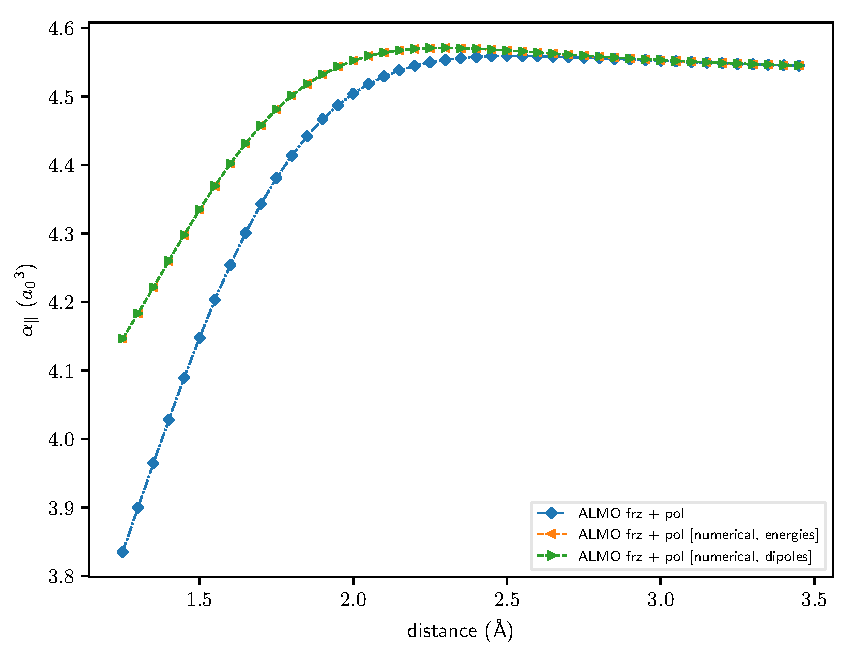
\includegraphics[scale=0.90]{paper_04/almo_analytic_vs_numerical_onaxis_projected_short_def2-SVP.pdf}
  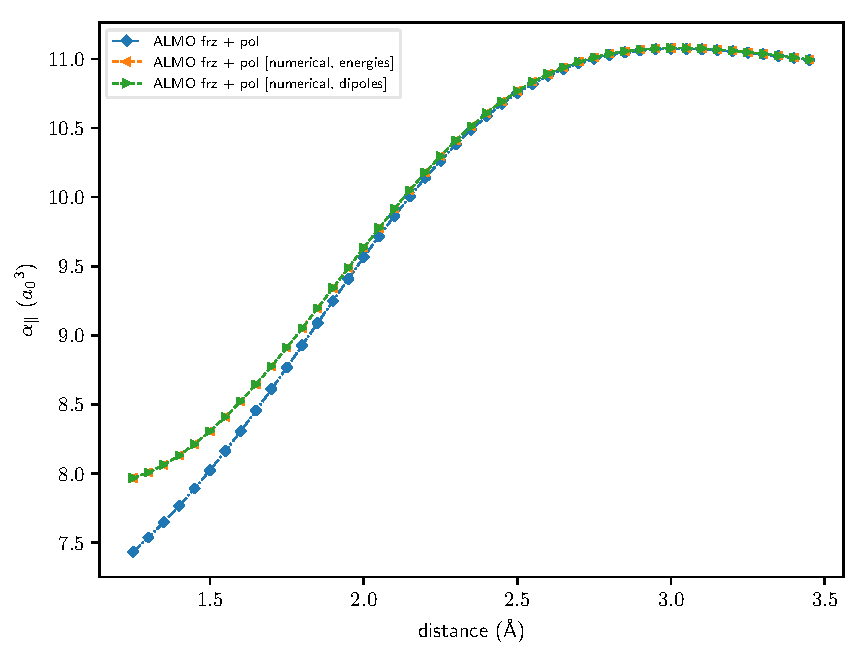
\includegraphics[scale=0.90]{paper_04/almo_analytic_vs_numerical_onaxis_projected_short_def2-SVPD.pdf}
  \caption[Distance dependence of analytic and numerical ALMO polarizabilities]{Distance dependence of analytic and numerical ALMO polarizabilities for both basis sets.}
  \label{fig:distance-dependence-validation}
\end{figure}

\begin{figure}
  \centering
  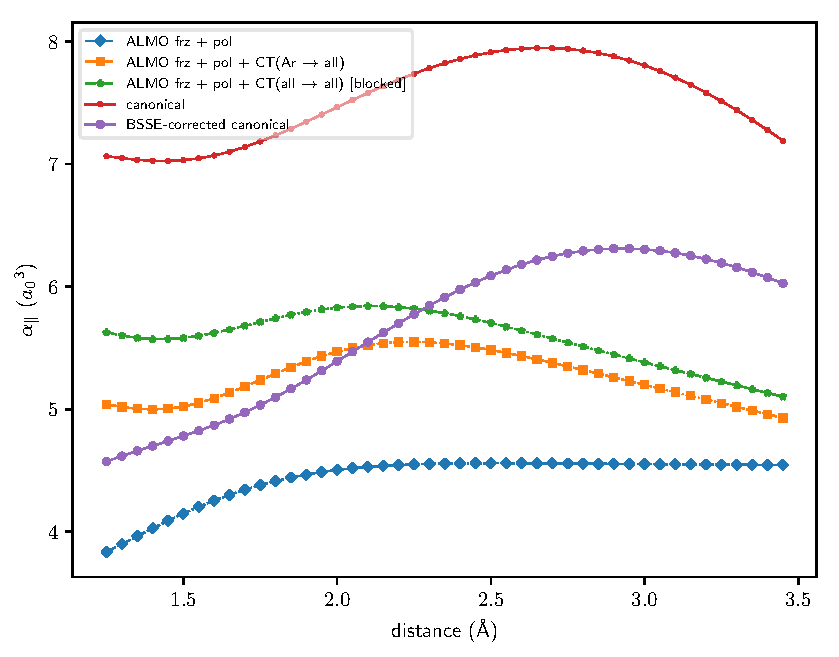
\includegraphics[scale=0.90]{paper_04/almo_vs_bsse_canonical_onaxis_projected_short_def2-SVP.pdf}
  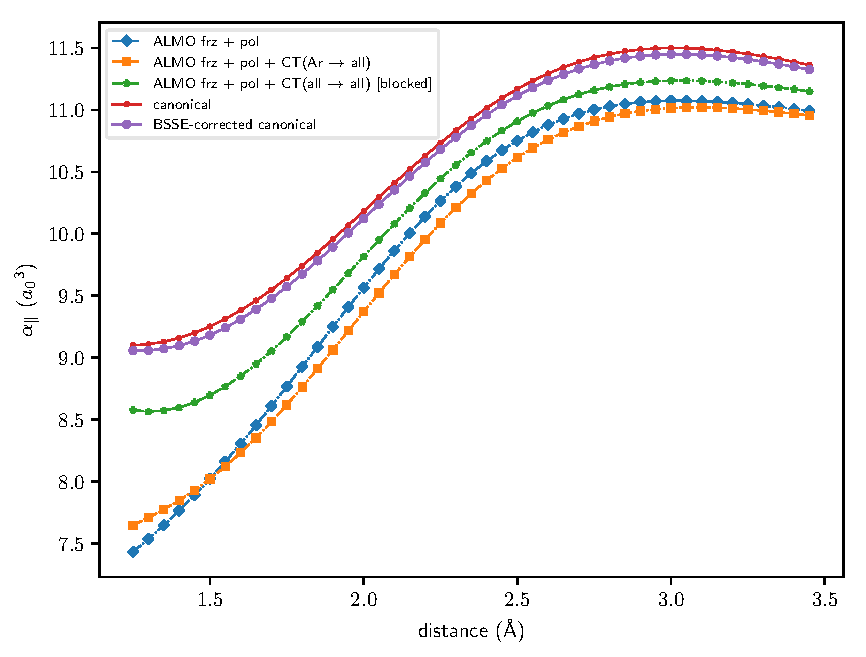
\includegraphics[scale=0.90]{paper_04/almo_vs_bsse_canonical_onaxis_projected_short_def2-SVPD.pdf}
  \caption[Distance dependence of CT restrictions on polarizabilities]{Distance dependence of CT restrictions on polarizabilities for both basis sets.}
  \label{fig:distance-dependence-ct-levels}
\end{figure}

Figure~\ref{fig:distance-dependence-ct-levels} shows how the different forms of CT restriction vary as a function of interatomic distance. Similar to the counterpoise (CP) correction for interaction energies, the ``BSSE-corrected canonical'' polarizability for two monomers A and B is defined as
\begin{equation}
  \alpha^{\text{BSSE-corrected}} = \alpha^{AB}(AB) - \left[ \left( \alpha^{A}(AB) - \alpha^{A}(A) \right) + \left( \alpha^{B}(AB) - \alpha^{B}(B) \right) \right],
  \label{eq:bsse-corrected-polarizability}
\end{equation}
where, for example, \(\alpha^{A}(AB)\) is the polarizability of monomer A in the combined (supermolecular) basis of both monomers.

The difference from the BSSE correction is large in def2-SVP but negligible in def2-SVPD, confirming our results from section~\ref{sssec:basis-set-dependence}. For both basis sets, the argon polarizability is the major contributor, provided that the entire dimer basis virtual space is available. The difference between the argon and blocked ALMO curves is due to the small but non-zero polarizability of the lithium cation, plus a mutual or higher-order polarization effect that appears at shorter than equilibrium distances for def2-SVP. Most notably, there is a quantitative difference between the blocked ALMO and canonical results even with def2-SVPD, showing that the wavefunction mechanism is large, and only allowing CT during the response calculation cannot recover these effects.

\section{\texorpdfstring{\caps{Conclusions and Future Work}}{Conclusions and Future Work}}
\label{sec:conclusions-and-future-work}

We have presented an implementation of linear response molecular properties for ALMOs, along with a decomposition of charge transfer effects, applied to a system with a substantial CT interaction. We discovered that for the static polarizability, charge transfer plays an equally important role in the response calculation as it does in the underlying wavefunction. Additionally, our results confirm that the ALMO and LR(MI) approximations are valid as long as the basis set is not deficient for the system, as is the case with def2-SVP.

A question not addressed in this work or other ALMO-based work on excitation energies\cite{Closser_2015_5791,doi:10.1063/1.4926837} is the effect of non-locality on the projected virtual space. To properly assign fragment-localized contributions to molecular response, both the occupied and virtual ALMOs must be spatially localized to individual fragments. Projecting the occupied space out of the virtual space ensures occupied-virtual orthogonality between fragments, but removes the fragment locality of the virtual space; that is, each virtual MO can no longer be uniquely assigned to a specific fragment. However, we expect that the error introduced by a delocalized virtual space is small compared to the error from using unprojected orbitals, which are less representative of the true potential energy surface for the reasons discussed in section~\ref{ssec:almo-adaptation}. Future work will use LoProp-type approaches on top of projected ALMOs to investigate the magnitude of these effects. In this way, LR(MI) can be a sensitive test for how modification of the virtual space affects molecular properties.

Our development of a library for calculating molecular response properties of arbitrary operators with non-orthogonal orbitals opens many doors for future development. \libresponse{} is available in \qchem{} 5.0.2 and at \url{https://github.com/LambrechtLab/libresponse} under the 3-clause BSD license as an Armadillo-based\cite{armadillo} C++ library. It can also be used as a \psif{}\cite{Psi41.1} plugin.

\section{\texorpdfstring{\caps{Acknowledgements}}{Acknowledgements}}

E.J.B. thanks \qchem{} for a summer internship opportunity, Evgeny Epifanovsky for help with the initial DIIS implementation, and cclib\cite{OBoyle:2008cc,eric_berquist_2016_60670} for the analysis framework.

\section{\texorpdfstring{\caps{Supporting Information}}{Supporting Information}}

ALMO-EDA results and analysis, additional ghost basis and point charge analysis, additional distance dependence results, sample input files, pseudocode for algorithm.

\begin{table}
  \centering
  \caption[ALMO-EDA results for argon\textemdash{}lithium cation dimer]{ALMO-EDA results. Energy units are \si{\kcal\per\mol}. All calculations used Hartree-Fock with a bond length of \SI{2.4297}{\angstrom}.}
  \label{tab:almo-eda-results}
  \begin{tabular}{ccc}
\toprule
& \multicolumn{2}{c}{basis set} \\
ALMO-EDA term & def2-SVP & def2-SVPD \\
\midrule
\(\Delta E_{\textrm{frz}}\) & 1.20 & 2.18 \\
\(\Delta E_{\textrm{pol}}\) & -3.32 & -6.61 \\
\(\Delta E_{\textrm{del}}^{\textrm{RS}}\) & -4.07 & -0.89 \\
\(\Delta E_{\textrm{BSSE}}^{\textrm{RS}}\) & 1.38 & 0.16 \\
\(\Delta E_{\textrm{CT}}^{\textrm{RS}}\) & -2.69 & -0.74 \\
\(\Delta E_{\textrm{int}}^{\textrm{RS}}\) & -4.81 & -5.17 \\
\(\Delta E_{\textrm{del}}^{\textrm{SCF}}\) & -5.38 & -1.08 \\
\(\Delta E_{\textrm{BSSE}}^{\textrm{SCF}}\) & 1.79 & 0.16 \\
\(\Delta E_{\textrm{CT}}^{\textrm{SCF}}\) & -3.59 & -0.91 \\
\(\Delta E_{\textrm{int}}^{\textrm{SCF}}\) & -5.70 & -5.35 \\
\(\Delta E_{\textrm{HO}}^{\textrm{SCF}}\) & -0.90 & -0.18 \\
\bottomrule
\end{tabular}

\end{table}

\begin{table}
  \centering
  \caption{Analysis of ALMO-EDA terms from table~\ref{tab:almo-eda-results}.}.
  \label{tab:almo-eda-results-percentages}
  \begin{tabular}{ccc}
\toprule
& \multicolumn{2}{c}{basis set} \\
& def2-SVP & def2-SVPD \\
\midrule
\(\Delta E_{\textrm{pol}}\) + \(\Delta E_{\textrm{CT}}^{\textrm{RS}}\) (kcal/mol) & -6.01 & -7.34 \\
\(\Delta E_{\textrm{pol}}\) + \(\Delta E_{\textrm{CT}}^{\textrm{SCF}}\) (kcal/mol) & -6.91 & -7.52 \\
100 * \(\Delta E_{\textrm{BSSE}}^{\textrm{RS}}\) / \(\Delta E_{\textrm{CT}}^{\textrm{RS}}\) (\%) & -51.4 & -21.2 \\
100 * \(\Delta E_{\textrm{BSSE}}^{\textrm{SCF}}\) / \(\Delta E_{\textrm{CT}}^{\textrm{SCF}}\) (\%) & -49.9 & -17.7 \\
100 * \(\Delta E_{\textrm{CT}}^{\textrm{RS}}\) / (\(\Delta E_{\textrm{pol}}\) + \(\Delta E_{\textrm{CT}}^{\textrm{RS}}\)) (\%) & 44.8 & 10.0 \\
100 * \(\Delta E_{\textrm{CT}}^{\textrm{SCF}}\) / (\(\Delta E_{\textrm{pol}}\) + \(\Delta E_{\textrm{CT}}^{\textrm{SCF}}\)) (\%) & 51.9 & 12.2 \\
\bottomrule
\end{tabular}

\end{table}

\begin{table}
  \centering
  \caption[Point charge and ghost function polarizability analysis]{Percentage of supermolecular result for point charge and ghost function polarizabilities. All calculations used Hartree-Fock with canonical MOs and a distance of \SI{2.4297}{\angstrom} from argon to the other center(s).}
  \label{tab:basis-set-dependence-percentages}
  \begin{tabular}{llrrrrr}
\toprule
 basis set &                          structure & \(\alpha_{\perp}\) & \(\alpha_{\parallel}\) & \(\bar{\alpha}\) & \(^{\text{t}}E_{0 \rightarrow \text{lowest}}^{\text{RPA}}\) & \(^{\text{s}}E_{0 \rightarrow \text{lowest}}^{\text{RPA}}\) \\
\midrule
  def2-SVP &   \ce{Ar\bond{....}PC(\mathrm{-})} &               84.1 &                   55.2 &             71.6 &                                                       195.5 &                                                       206.0 \\
  def2-SVP &                            \ce{Ar} &               83.9 &                   55.5 &             71.6 &                                                       199.1 &                                                       209.4 \\
  def2-SVP &   \ce{Ar\bond{....}PC(\mathrm{+})} &               83.7 &                   55.6 &             71.6 &                                                       196.8 &                                                       207.2 \\
  def2-SVP &  \ce{Ar\bond{....}\mathrm{Gh}(Li)} &               93.9 &                   79.1 &             87.5 &                                                       103.0 &                                                       103.3 \\
 def2-SVPD &   \ce{Ar\bond{....}PC(\mathrm{-})} &              108.6 &                   93.4 &            103.3 &                                                        91.2 &                                                        94.7 \\
 def2-SVPD &                            \ce{Ar} &              103.0 &                   93.8 &             99.7 &                                                       105.3 &                                                       107.1 \\
 def2-SVPD &   \ce{Ar\bond{....}PC(\mathrm{+})} &               99.7 &                  108.0 &            102.6 &                                                        82.6 &                                                        84.9 \\
 def2-SVPD &  \ce{Ar\bond{....}\mathrm{Gh}(Li)} &              103.2 &                   94.2 &            100.0 &                                                       100.6 &                                                       100.6 \\
\bottomrule
\end{tabular}

\end{table}

\begin{figure}
  \centering
  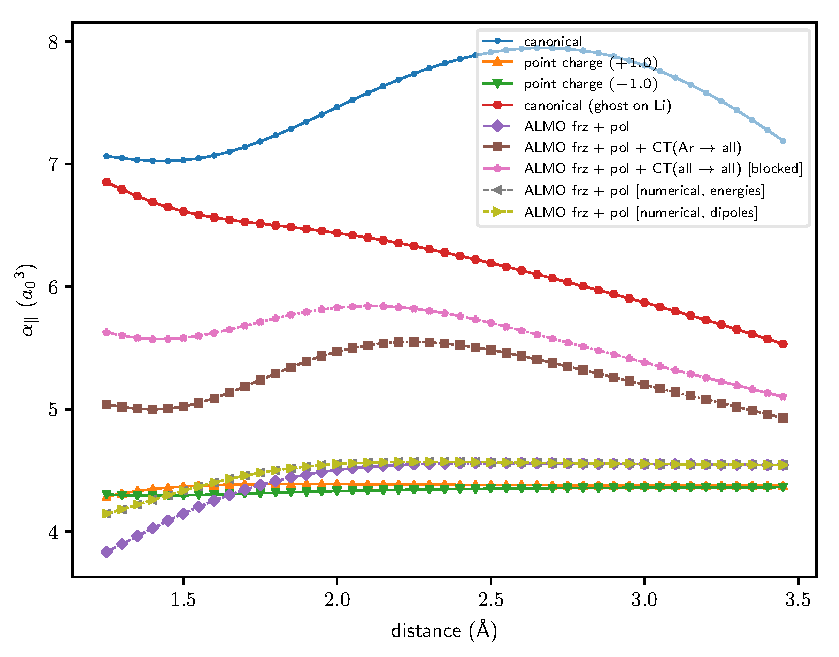
\includegraphics[scale=0.90]{paper_04/polar_onaxis_projected_short_def2-SVP.pdf}
  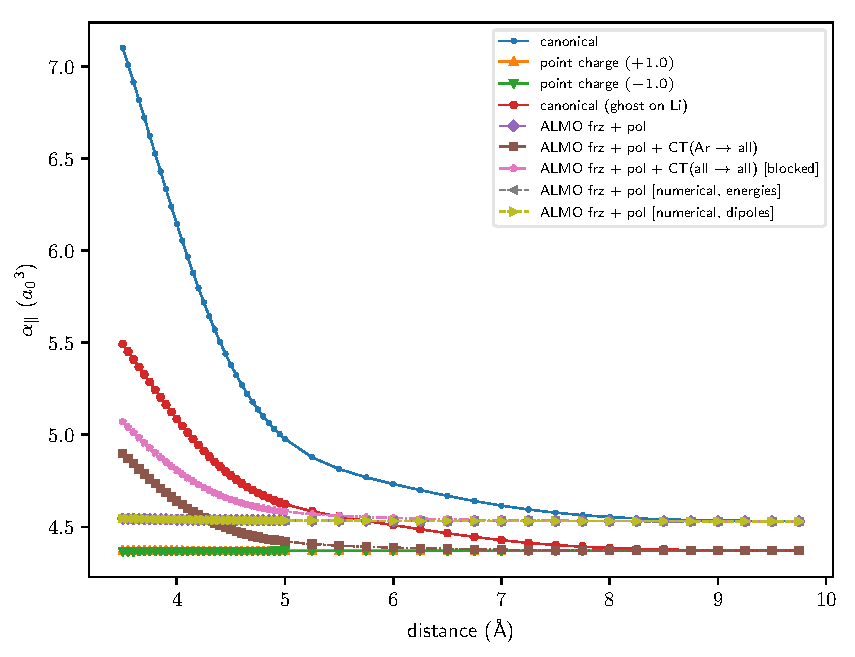
\includegraphics[scale=0.90]{paper_04/polar_onaxis_projected_long_def2-SVP.pdf}
  \caption[Distance dependence of \(\alpha_{\parallel}\) for def2-SVP]{Short- and long-range interatomic separation dependence of the static polarizability parallel to the coordination axis. All calculations are at the HF/def2-SVP level.}
  \label{fig:distance-dependence-parallel-def2-svp}
\end{figure}

\begin{figure}
  \centering
  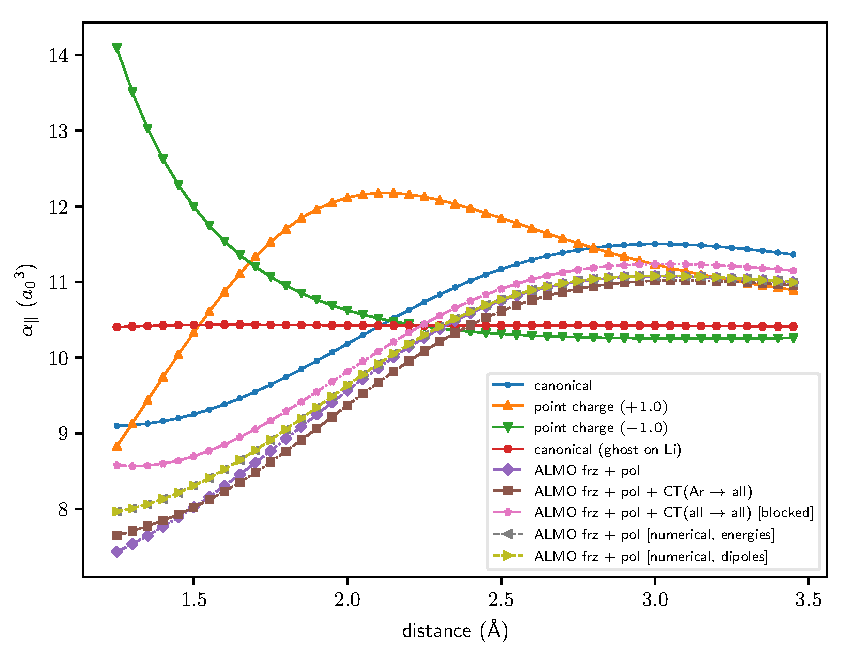
\includegraphics[scale=0.90]{paper_04/polar_onaxis_projected_short_def2-SVPD.pdf}
  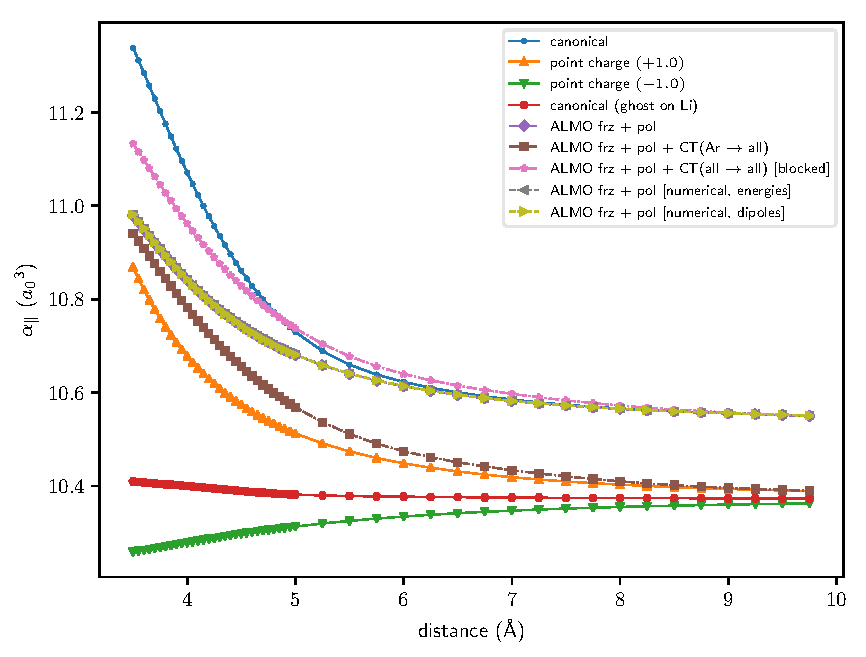
\includegraphics[scale=0.90]{paper_04/polar_onaxis_projected_long_def2-SVPD.pdf}
  \caption[Distance dependence of \(\alpha_{\parallel}\) for def2-SVPD]{Short- and long-range interatomic separation dependence of the static polarizability parallel to the coordination axis. All calculations are at the HF/def2-SVPD level.}
  \label{fig:distance-dependence-parallel-def2-svpd}
\end{figure}

\begin{figure}
  \centering
  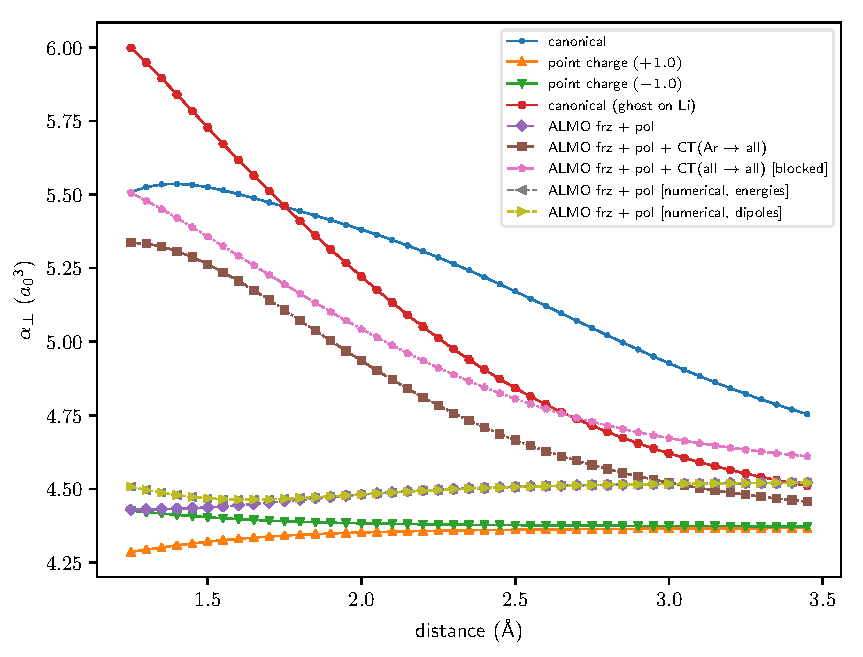
\includegraphics[scale=0.90]{paper_04/polar_offaxis_projected_short_def2-SVP.pdf}
  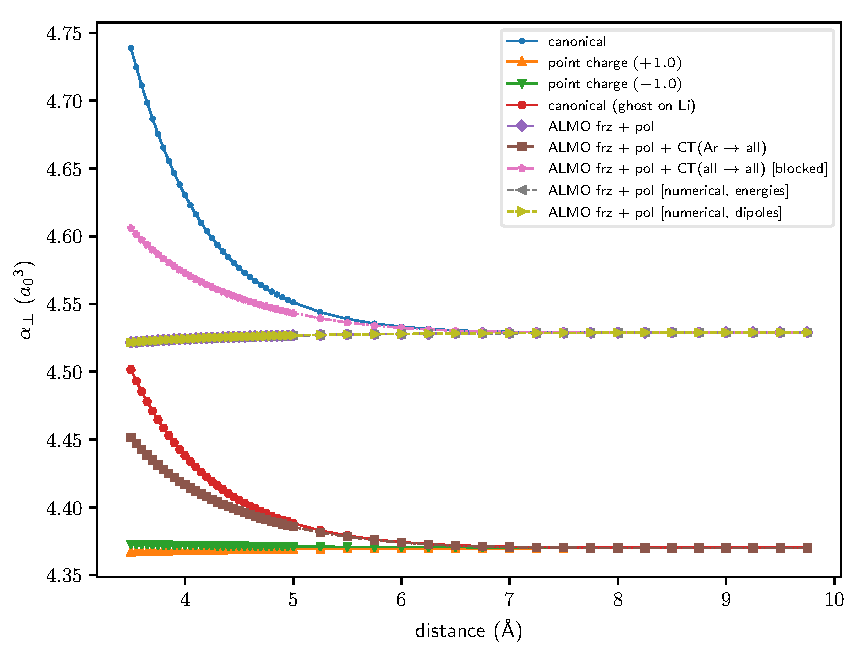
\includegraphics[scale=0.90]{paper_04/polar_offaxis_projected_long_def2-SVP.pdf}
  \caption[Distance dependence of \(\alpha_{\perp}\) for def2-SVP]{Short- and long-range interatomic separation dependence of the static polarizability perpendicular to the coordination axis. All calculations are at the HF/def2-SVP level.}
  \label{fig:distance-dependence-perp-def2-svp}
\end{figure}

\begin{figure}
  \centering
  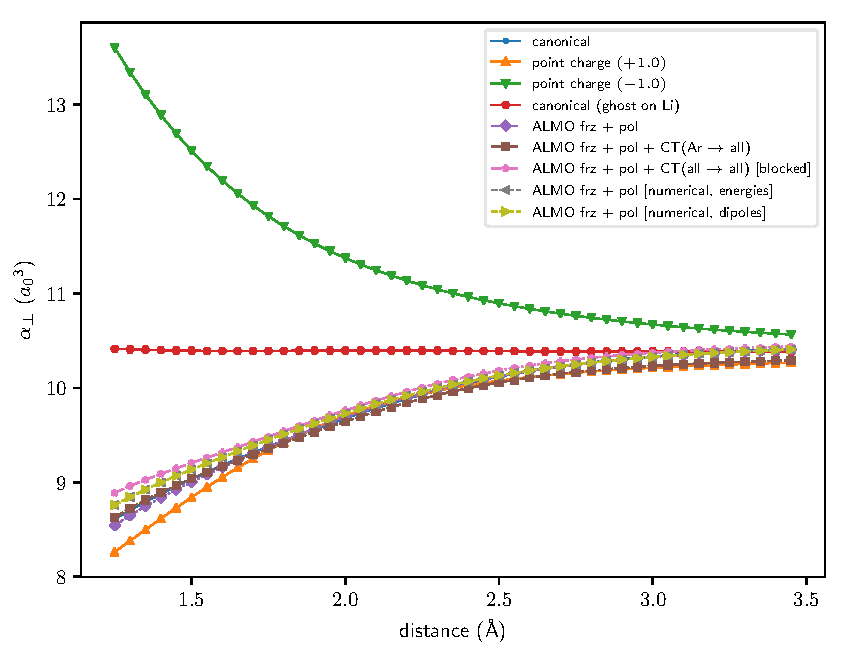
\includegraphics[scale=0.90]{paper_04/polar_offaxis_projected_short_def2-SVPD.pdf}
  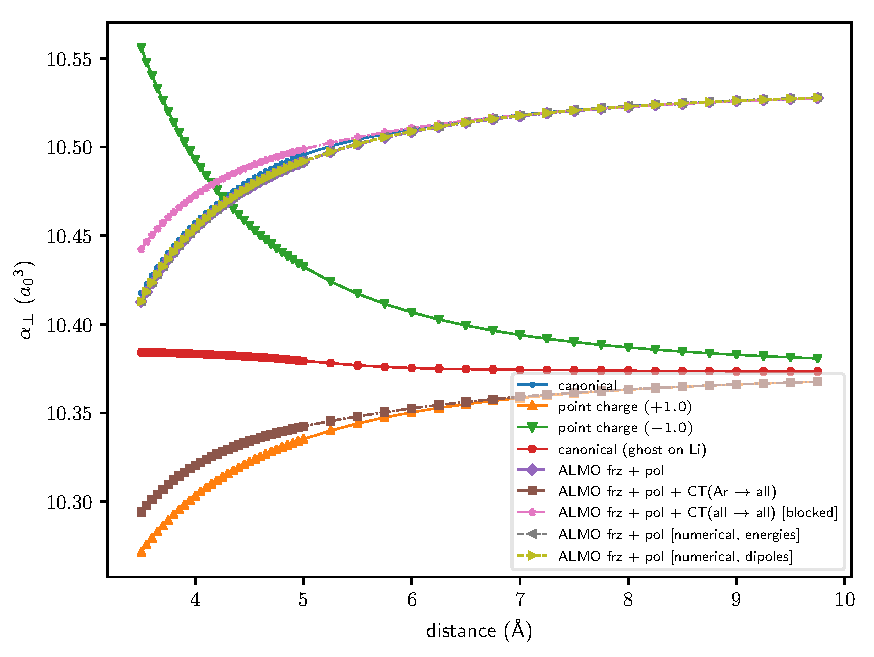
\includegraphics[scale=0.90]{paper_04/polar_offaxis_projected_long_def2-SVPD.pdf}
  \caption[Distance dependence of \(\alpha_{\perp}\) for def2-SVPD]{Short- and long-range interatomic separation dependence of the static polarizability perpendicular to the coordination axis. All calculations are at the HF/def2-SVPD level.}
  \label{fig:distance-dependence-perp-def2-svpd}
\end{figure}

As a sanity check for all results, we expect certain physical behavior over the range of interatomic distances. In particular, as the interatomic distance approaches the limit of infinite separation,

\begin{itemize}
\item The canonical SCF, numerical SCF(MI), and analytic SCF(MI) results all converge to the same value, which is the sum of polarizabilities the two isolated atoms. CT appears to be an important contributor until approximately \SI{5}{\angstrom}, where the decay behavior of the canonical SCF changes.
\item The point charge, and ``frz + pol + CT(\ce{Ar} \(\rightarrow\) all)'' results all converge to the same value, which is the polarizability of the isolated argon atom.
\end{itemize}

\subsection{Input files}

\lstinputlisting[%
label=listing:input-polarizability,%
caption=Sample \qchem{} input file for ``ALMO frz + pol'' polarizability. Geometry is from HF/def2-SVPD.%
]{paper_04/almo_stoll_projvirts_restricted.in}

Using the template from listing~\ref{listing:input-polarizability}:

\begin{itemize}
\item To perform the ``ALMO frz + pol + CT(all \(\rightarrow\) all) [blocked]'' calculations, set \lstinline|_frgm_response_idx = 0| and all \lstinline|_mask_*| options to \lstinline|false|.
\item To perform the ``ALMO frz + pol + CT(Ar \(\rightarrow\) all)'' calculations, set \lstinline|_frgm_response_idx = 1| and all \lstinline|_mask_*| options to \lstinline|true|.
% \item For the perturbative correction calculations (``ALMO frz + pol + CT(all \(\rightarrow\) all) [RS]''), an input file is identical to ``ALMO frz + pol + CT(all \(\rightarrow\) all) [blocked]'' with \lstinline|solver = linear|, \lstinline|maxiter = 1|, and \lstinline|conv = -1|;
% \item For the uncoupled ALMO calculations, an input file is identical to ``ALMO frz + pol + CT(all \(\rightarrow\) all) [blocked]'' with \lstinline|solver = diis|, \lstinline|maxiter = 1|, and \lstinline|conv = -1|.
% \item For the uncoupled canonical calculations, an input file is identical to a canonical calculation with \lstinline|solver = diis|, \lstinline|maxiter = 1|, and \lstinline|conv = -1|.
\end{itemize}

\lstinputlisting[%
label=listing:input-almo-eda-gen1,%
caption=Sample \qchem{} input file for first-generation ALMO-EDA. Geometry is from HF/def2-SVPD.%
]{paper_04/eda_bsse_def2-SVPD.in}

\lstinputlisting[%
label=listing:input-almo-eda-gen2,%
caption=Sample \qchem{} input file for second-generation ALMO-EDA. Geometry is from HF/def2-SVP.%
]{paper_04/eda2_1_scf_nobsse_def2-SVPD.in}

\subsection{Algorithm description}

\algnewcommand\Break{\textbf{break}}
\algnewcommand\Not{\textbf{not}}
\algnewcommand\True{\textbf{true}}
\algnewcommand\False{\textbf{false}}
\algnewcommand\Rhsvecs{\textsf{rhsvecs}}
\algnewcommand\Rspvecs{\textsf{rspvecs}}
\algnewcommand\Operators{\textsf{operators}}
\algnewcommand\Resp{\textsf{resp}}
\algnewcommand\AllowCT{\textsf{allow\_ct?}}

\begin{algorithm}
  \centering
  \begin{algorithmic}[1]
  \Procedure{solve\_linear\_response}{\Resp, \Operators, occupations, \(\mat{C}, \mat{F}, \mat{S}, \vartheta\), maxiter, \AllowCT}
  \For{\(s \gets 1, N_{spin}\)}
    \State Transformation of \(\mat{F}\) and \(\mat{S}\) from AO to full MO basis
    \State \(E_{ia,jb} = F_{ab}S_{ij} - F_{ij}S_{ab}\)
    \Comment{Form non-orthogonal orbital energy matrix \(\mat{E}\)}
    \If{\Not{} \AllowCT{}}
      \State Zero cross-fragment \(ia\) indices and shrink dimensions of \(\mat{E}\)
    \EndIf
    \State Form inverse for denominator \(\mat{E}^{-1}\)
  \EndFor
  \For{\(i \gets 1, N_{operators}\)}
    \For{\(c \gets 1, N_{components}\)}
      \State \((\mat{Z})_{\mu\nu} \gets \Operators[i,c,\mu\nu]\)
      \Comment{Select operator component as perturbation for right-hand side}
      \State Transform operator component from AO to occ-virt MO basis and append \(\mat{Z}_{ia}\) to \Rhsvecs
      \If{\Not{} \AllowCT{}}
        \State Zero cross-fragment \(ia\) indices and shrink dimensions of \(\mat{Z}\)
      \EndIf
      \State \(\mat{X}^{(0)} \gets \mat{0}\)
      \Comment{Form initial guess for response vector (uncoupled result)}
      \State \(converged \gets \False\)
      \For{\(n \gets 1, maxiter\)}
        \State \(D_{\mu\nu}^{X} \gets C_{\mu i} X_{ia}^{(n-1)} C_{\nu a}\)
        \Comment{Form perturbed density}
        \State \(J_{\mu\nu}^{X}\left[\mat{D}^{X}\right], K_{\mu\nu}^{X}\left[\mat{D}^{X}\right] \gets fock\_build(\mat{D}^{X})\)
        \Comment{Form Coulomb and exchange contributions}
        \State \(\left(\mat{R}^{(n)}\right)_{\mu\nu} \gets 4 \mat{J}^{X} - \mat{K}^{X} - \left(\mat{K}^{X}\right)^{T}\)
        \Comment{Form half-transformed orbital Hessian-vector product (here, \(\mat{G} = \mat{A}^{s} + \mat{B}^{s}\))}
        \State Do second transformation of Hessian-vector product \(\left(\mat{R}\right)_{ia}^{(n)}\)
        \If{\Not{} \AllowCT{}}
          \State Zero cross-fragment \(ia\) indices and shrink dimensions of \(\mat{R}, \mat{X}\)
        \EndIf
        \State \(X_{ia}^{(n)} \gets (\mat{E}^{-1})_{ia,jb} \left[ Z_{jb} - R_{jb}^{(n)} \right]\)
        \Comment{Update response vector}
        \If{\Not{} \AllowCT{}}
          \State Restore dimensions of \(\mat{X}\)
        \EndIf
        \If{\(||\mat{X}^{(n)} - \mat{X}^{(n-1)}|| < \vartheta\)}
          \State \(converged \gets \True\)
          \State Append \(\mat{X}^{(n)}\) to \Rspvecs
          \State \Break
        \EndIf
  \algstore{lrmi}
  \end{algorithmic}
  \caption{Static linear response approach within fragment-localized formalism.}
  \label{alg:solve-linear-response}
\end{algorithm}
\begin{algorithm}
  \centering
  \begin{algorithmic}[1]
  \algrestore{lrmi}
        \EndFor
      \If{\Not{} \(converged\)}
        \State crash
      \EndIf
    \EndFor
  \EndFor
  \State \(\Resp \gets \mat{0}\)
  \Comment{Form all possible permutations of property gradient and response vectors}
  \For{\(a \gets 1, len(\Rhsvecs)\)}
    \For{\(b \gets 1, len(\Rspvecs)\)}
      \State \(\mat{P} \gets \Rhsvecs[a], \mat{Q} \gets \Rspvecs[b]\)
      \State \(\lr{P}{Q}_{0} \gets -P_{ia}Q_{ia}\)
      \State \(\Resp[a,b] \gets \lr{P}{Q}_{0}\)
    \EndFor
  \EndFor
  \EndProcedure
  \end{algorithmic}
  \caption{Continuation of algorithm~\ref{alg:solve-linear-response}}
  \label{alg:solve-linear-response-2}
\end{algorithm}

Algorithm~\ref{alg:solve-linear-response}/\ref{alg:solve-linear-response-2} is the general outline of the LR(MI) procedure, without convergence acceleration. The key difference between our implementation and a general CPHF solver is the zeroing of vector and matrix elements. Again, any contraction between \(ia\) or \(ia,jb\) indices may be restricted, but transformations from \(\mu\nu\) to \(ia\) are not.

Missing from this example is the formation of \(\mat{A}, \mat{B}\), and the prefactor in the equation for real/imaginary operators. A difference from the paper equations in the implementation is that rather than take a single \(\op{P}\) and single \(\op{Q}\), a list of operators is passed. For example, if \(\Operators = [\op{\mu}, \op{m}]\), then \(\lr{\mu}{\mu},\lr{\mu}{m}\), and \(\lr{m}{m}\) will automatically be formed. Another implementation detail is that each operator carries its own property gradient vectors (the occ-virt MO basis integrals for the right-hand side) and perturbed response vectors, and each operator carries information about whether it is real/imaginary and spin conserving/altering.

\newcommand{\numpy}{{\textsc{NumPy}}\xspace}%
\newcommand{\pfour}{{\textsc{Psi4}}\xspace}%
\newcommand{\pfn}{{\textsc{Psi4NumPy}}\xspace}%

\chapter[\pfn]{\pfn: An Interactive Quantum Chemistry Programming Environment for Reference Implementations and Rapid Development}
\label{ch:paper_05}

The text in this chapter has been adapted from

\section{Chapter Summary}

\section{Introduction}

Whereas in the past a new quantum chemical (QC) method was commonly presented solely through its equations, perhaps along with a few token values, the more recent expectation is that equations will be accompanied by results from an effective computer program clearly demonstrating the utility of the method.  This expectation becomes increasingly burdensome as new computer architectures emerge, since some theories will be naturally more computationally efficient or more difficult to implement than others.  The computation expense of most quantum chemical methods creates substantial pressure for methods to be implemented with highly optimized algorithms.

This situation presents a challenge for ongoing development in quantum chemistry, because new theoretical methods are typically complex and their correct implementation is non-trivial.  Additionally, computationally efficient codes require a low-level programming language like C++ or Fortran, followed by substantial code profiling, testing, and optimization.  Often a method's first implementation is a rather messy computer program. The researcher may be learning the details of the method as they progress, resulting in ``experimental'' parts of the code that may never get removed, or data structures that may not be optimal for the final version of the method.  Additionally, development is often carried out by graduate students not yet proficient in programming, resulting in unconventional coding styles.  Subsequently, a researcher seeking to extend or enhance a method previously developed in-house is often faced with the daunting prospect of deciphering a quite complex existing code.

Still more challenging is implementing or extending an existing method sourced solely from the literature.  Often, a paper describing a new quantum chemical method that properly focuses on scientific detail falls short on algorithmic or numerical detail sufficient for independent reimplementation. Indeed, the methods are so complex that the original equations frequently include typos, which are generally tracked through institutional lore rather than published errata.  Additionally, modern approaches often employ combinations of approximations with multiple numerical cutoffs, exacerbating the reproducibility problem.  This paradigm is illustrated within a recent comment,\cite{Briling:2017:157101} whereby several corrections to equations originally published in 2011 for a two-level semi-empirical method\cite{Laikov:2011:134120} were proposed after being re-engineered to reproduce values computed using a binary program distributed with the original publication.  Even facilitated through private communication with the method's author, this cycle of rediscovery and reimplementation is both highly non-trivial and unsustainable.  Fortunately, an open-source program\cite{brilingqm} has been made available by the commenting author that implements the method and proposed changes, so that further extensions of the method can proceed with this program as a reference.

Such ``reference implementations'' (easy-to-read, unoptimized computer programs solely targeting the correct result) can be a helpful initial step toward developing or understanding a complex method, yet they are not widely available in quantum chemistry.  To our knowledge, reference implementations and benchmarking have only been performed in a large-scale way for density functional theory (DFT) exchange-correlation kernels\cite{CCL_DFT} and periodic boundary condition DFT with pseudopotentials.\cite{Lejaeghereaad3000} One factor limiting more widespread use of reference implementations for quantum chemistry is that methods are often so computationally demanding that a basic, unoptimized implementation is too slow for computations on even the smallest molecules.  What is needed is an alliance of QC code that is easy to peruse and manipulate with underlying non-QC routines that are fast enough for testing on non-trivial molecules.

Here we present \pfn, a framework for the creation of clear, readable reference implementations of quantum chemical methods and for the rapid development of new methods. \pfn takes advantage of \pfour's\cite{Psi41.1} application programming interface (API) that makes efficient computational kernels written in C++ available from Python, a language that is easy to learn and has become very popular in scientific computing.  As a high-level language, Python allows complex tasks to be specified with relatively few lines of code.  \pfn capitalizes on the straightforward conversion of \pfour tensors to \numpy\cite{Varoquaux:1521-9615} and Numerical Python's (\numpy's) own low-level back end to ensure that all data arrays can use the optimized Basic Linear Algebra Subroutines (BLAS) library\cite{BLAS} for common linear algebra operations. The wide user base of \numpy ensures constant updates and bug fixes. \pfn has been packaged for minimal setup, requiring only 3 minutes, with no preinstalled compilers necessary on 64-bit Linux, Mac, and Windows.  Here we introduce the main elements of the \pfn framework and illustrate them with a substantial collection of reference implementations for standard quantum chemical methods and numerical techniques. The \pfn is built entirely on Free and Open Source Software (FOSS)\cite{FOSS} as shown in Fig.~\ref{fig:ovalorg} to ensure a barrierless entry to quantum chemistry programming.

Several of the reference implementations have been augmented by tutorial-style introductions to the relevant theory.  The \pfn tutorial collection includes self-consistent field (SCF), DFT,\cite{Parr:1989} many-body perturbation theory (MBPT),\cite{Bartlett:1981:359} symmetry-adapted perturbation theory (SAPT)\cite{Jeziorski:1994:1887, Szalewicz:2012:254}, coupled-cluster (CC)\cite{Purvis:1982}, and configuration interaction (CI)\cite{Shavitt:1977,Sherrill:1999:CI} theories, with additional sections detailing the theory and implementation of linear response, geometry optimizations, and Verlet integrators.  It is our hope that \pfn and the accompanying reference code will lower the barrier to implementing quantum chemical methods.

\begin{figure}
  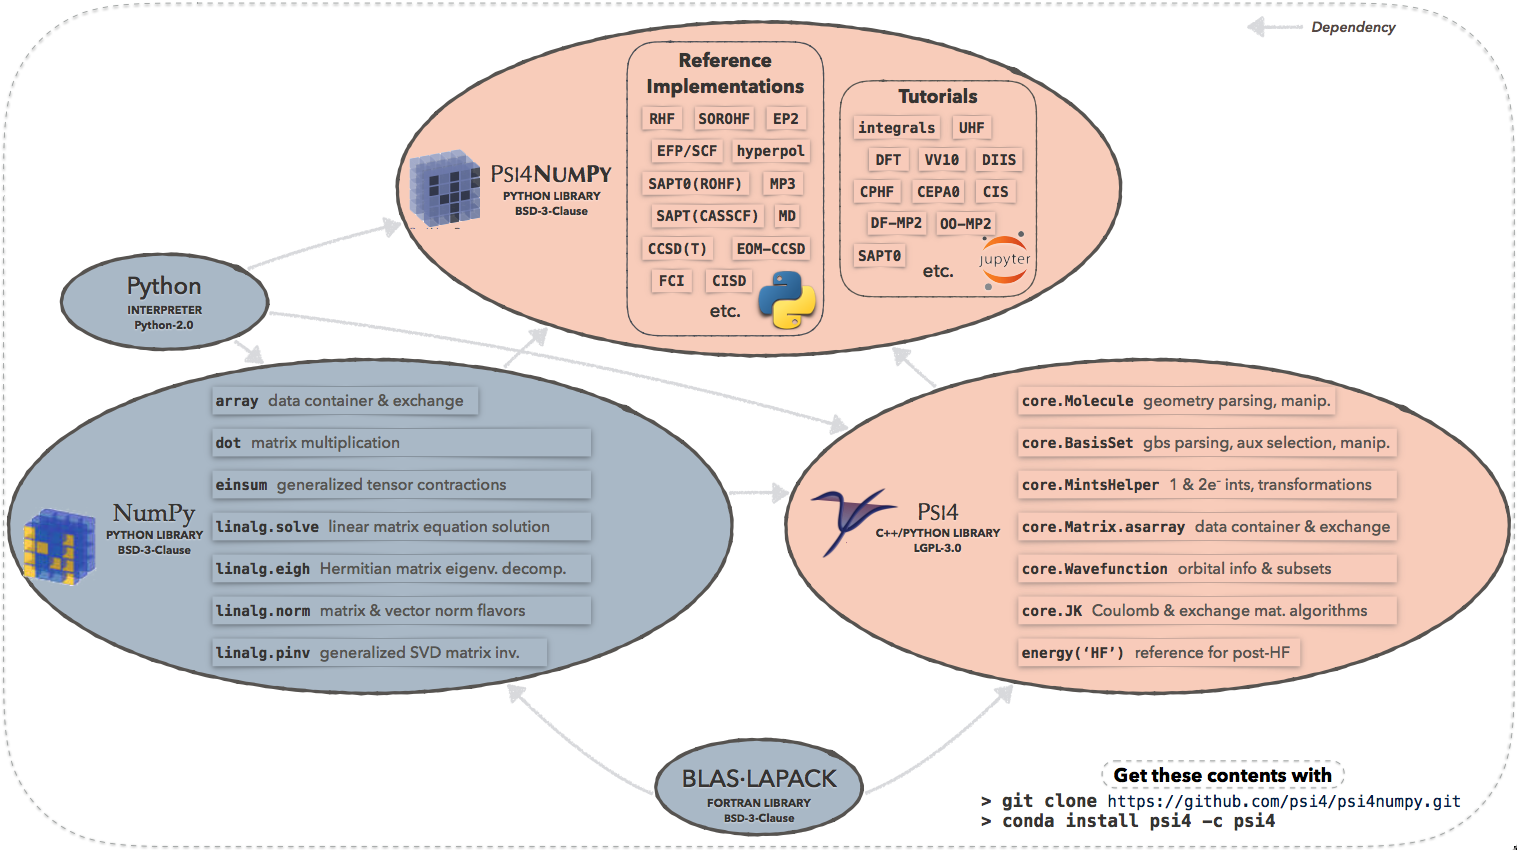
\includegraphics[width=\textwidth]{paper_05/fig1.png}
  \caption{\pfn draws linear algebra tools from \numpy and fundamental quantum chemistry structures from \pfour to bring together a practical and convenient environment for code development, verification, and exploration. The most important data structures and functions are shown for \numpy and \pfour as well as representative tutorial and reference implementations presently in \pfn.\label{fig:ovalorg}}
\end{figure}

Shortly before submission, the authors chanced upon the Quantum Chemistry Program Exchange (QCPE)\cite{QCPE, Boyd:2013:221}, whose goals of software (particularly self-contained software) accessibility, algorithm explication, and free software ``publishing'' \pfn shares. The general tools embraced by \pfn (GitHub for communication, \numpy for linear algebra, Python for interfacing, and Jupyter for illumination) further allow rapid prototyping and educational objectives. In this manner \pfn can be thought as a modern successor to QCPE built to serve the flexible needs of the community.

\section{Basic Tools}

The basic premise of \pfn is to leverage \pfour to generate quantum chemistry-specific quantities and the \numpy library\cite{Varoquaux:1521-9615} for all other tensor manipulations.  The latest version of \pfour has added the capability to import \pfour as a Python module as well as continuing to be called in an executable fashion. In this way, both the \pfour and \numpy libraries can be loaded into a single Python script and used in cooperation.

A key capacity in this enterprise is seamless translation between \numpy and \pfour data classes. For example, converting from a \numpy array to a \pfour matrix and back again can be easily accomplished:
\begin{eqnarray}
  \begin{aligned}
    &\verb!import numpy, psi4! \\[-10pt]
    &\verb!np_array = numpy.zeros((5, 5))! \\[-10pt]
    &\verb!psi4_matrix = psi4.core.Matrix.from_array(np_array)! \\[-10pt]
    &\verb!new_np_array = numpy.array(psi4_matrix)! \\[-10pt]
  \end{aligned}
  \label{snip:np2p42np}
\end{eqnarray}
%Refer as Eq.~\ref{snip:np2p42np}.
At the core of this procedure is \textsc{NumPy}'s {\tt array\_interface}\cite{array_interface} protocol, a basic specification for dense matrices consisting of
\begin{enumerate}
\item (a) the starting memory location for an in-memory array
\item (b) the overall ``shape'' of the array [$(n,)$ for a vector, $(n,m)$ for a matrix, etc.]
\item (c) the type of data involved (\texttt{double64}, \texttt{int32}, etc.)
\end{enumerate}
This specification is compact and widely used amongst the scientific Python community in a variety of scenarios. Using the {\tt array\_interface}, it becomes straightforward to allow \numpy access to a \pfour data class, allowing both \pfour and \numpy to access and manipulate the same data. For example, the below will overwrite the \pfour Matrix class in place with a random \numpy array:
\begin{eqnarray}
  \begin{aligned}
    &\verb!psi4_matrix.np[:] = numpy.random.rand(5, 5)! \\
  \end{aligned}
  \label{snip:numpy_set}
\end{eqnarray}
In this way the typical separation between general tensor frameworks and custom quantum chemistry data structures is removed.

A description of the full set of capabilities of the {\tt array\_interface} is available in the \pfour documentation: \url{http://psicode.org/psi4manual/master/numpy.html}.

\subsection{Wavefunction Objects}

In \pfour all built-in methodologies have the option to return a Wavefunction object that holds basic information about the previous computation or, in some cases, holds functions for readily computing advanced quantities. Obtaining the Wavefunction object in this manner is straightforward:
\begin{eqnarray}
  \begin{aligned}
    &\verb!mol = psi4.geometry("""! \\[-10pt]
    &\verb!O! \\[-10pt]
    &\verb!H 1 0.96! \\[-10pt]
    &\verb!H 1 0.96, 104.5! \\[-10pt]
    &\verb!""")! \\
    &\verb!hf_e, hf_wfn = psi4.energy("HF/cc-pVDZ", molecule=mol, return_wfn=True)! \\
  \end{aligned}
  \label{snip:scf_computation}
\end{eqnarray}
Once a Wavefunction object is obtained, a variety of attributes can be queried
using standard Python syntax:
\begin{eqnarray}
  \begin{aligned}
    &\verb!# Number of doubly occupied orbitals!\\[-10pt]
    &\verb!docc = hf_wfn.ndocc() !\\
    &\verb!# Alpha orbital coefficient matrix !\\[-10pt]
    &\verb!Ca = hf_wfn.Ca() !\\
    &\verb!# Occupied subset of the alpha orbitals !\\[-10pt]
    &\verb!Ca_occ = hf_wfn.Ca_subset("AO", "OCC") !
  \end{aligned}
      \label{snip:wfn_data}
\end{eqnarray}
In addition to generating useful information after a computation, a Wavefunction object can also be passed as reference state to a further computation.  For \pfn, this means that reference implementations of post-Hartree--Fock methods (MPn, CCSD, etc.) need not re-code their own Hartree--Fock program; this simultaneously reduces code duplication and increases readability, both of which are cornerstones of the \pfn project.

% In particular, SCF Wavefunctions also have the ability to obtain SCF (Hartree-Fock) level quantities. For example, using a SCF Wavefunction one can "step" through the iterations by successively calling the Roothan-Hall equations:

% \begin{verbatim}
% form_C() # Forms the orbital matrix from the current Fock matrix
% form_D() # Forms the density matrix from the current orbital matrix
% form_F() # Forms the Fock matrix from the current density matrix.
% \end{verbatim}

% To better acquaint users with the Python-exposed functions of all Psi4 classes, use the built-in Python {\tt help} function. For example, using the above Wavefunction object:

%\begin{verbatim}
%>>> help(hf_wfn)
% |  Methods inherited from HF (Hartree-Fock):
% |  form_C(...) from builtins.PyCapsule
% |      form_C(self: psi4.core.HF) -> None
% |
% |      Forms the Orbital Matrices from the current Fock Matrices.
% |
% |  form_D(...) from builtins.PyCapsule
% |      form_D(self: psi4.core.HF) -> None
% |
% |      Forms the Density Matrices from the current Orbitals Matrices
%  ...
% |  Methods inherited from Wavefunction:
% |
% |  Ca(...) from builtins.PyCapsule
% |      Ca(self: psi4.core.Wavefunction) -> psi4.core.Matrix
% |
% |      Returns the Alpha Orbitals.
% |
% |  S(...) from builtins.PyCapsule
% |      S(self: psi4.core.Wavefunction) -> psi4.core.Matrix
% |
% |      Returns the One-electron Overlap Matrix.
%\end{verbatim}

\subsection{Integrals}

\pfour offers a wide selection of efficient C++ tools accessible directly in Python.  These tools are largely object-based and capable of storing quantities in memory or on disk.  One such object is the \texttt{libmints} library\cite{Psi41.1}, which is currently the primary interface for computing one- and two-electron integrals in \pfour.  This library is accessible through the \texttt{MintsHelper} class that directs the efficient computation and storage of molecular integrals Python-side:
\begin{eqnarray}
  \begin{aligned}
    &\verb!# Create instance of MintsHelper using primary basis set !\\[-10pt]
    &\verb!mints = psi4.core.MintsHelper(primary_basis) !\\
    &\verb!# Compute one-electron AO overlap matrix !\\[-10pt]
    &\verb!S = mints.ao_overlap() !\\
    &\verb!# Compute core Hamiltonian matrix !\\[-10pt]
    &\verb!T = mints.ao_kinetic() !\\[-10pt]
    &\verb!V = mints.ao_potential() !\\[-10pt]
    &\verb!H = T + V !\\
    &\verb!# Compute two-electron integrals in AO basis in memory !\\[-10pt]
    &\verb!I_ao = mints.ao_eri() !
  \end{aligned}
      \label{snip:mints}
\end{eqnarray}
Each of the above \texttt{MintsHelper} class methods returns a \pfour matrix which can be converted to a \numpy array using \texttt{numpy.asarray(matrix)} or modified in place with the \texttt{matrix.np} accessor.

In addition to computing molecular integrals, the \texttt{libmints} library also performs optimized electron repulsion integral (ERI) transformations. For example, the ${\cal O}(N^5)$ transformation of the two-electron integrals between the atomic orbital and molecular orbital basis, given by
\begin{equation}
  (ia\vert jb) = \left[\left[C_{\mu i}\left[C_{\nu a}(\mu\nu\vert\lambda\sigma)\right]\right]C_{\lambda j}\right]C_{\sigma b},
  \label{eq:aomo}
\end{equation}
can be performed easily with:
\begin{eqnarray}
  \begin{aligned}
    &\verb!# Occupied and virtual subsets of SCF orbital coefficient matrices !\\[-10pt]
    &\verb!Ca_occ = hf_wfn.Ca_subset("AO", "OCC") !\\[-10pt]
    &\verb!Ca_virt = hf_wfn.Ca_subset("AO", "VIR") !\\
    &\verb!# AO basis to MO basis in-memory ERI transform !\\[-10pt]
    &\verb!I_mo = mints.mo_transform(Ca_occ, Ca_virt, I_ao, Ca_occ, Ca_virt) !\\
  \end{aligned}
  \label{snip:eri_trans}
\end{eqnarray}
In this manner, arbitrary ERI transformations may be performed, allowing both speed and flexibility for constructing reference implementations.

\subsection{Coulomb and Exchange (JK) Matrix Objects}

A key component in SCF-level theories is the contraction of the 4-index electron repulsion integrals with the 2-index density matrix to form $J$ and $K$ matrices:
\begin{eqnarray}
  J_{\lambda \sigma}[D] &\equiv& (\lambda\sigma|\mu\nu) D_{\mu\nu}, \\
  K_{\lambda \sigma}[D] &\equiv& (\lambda\mu|\sigma\nu) D_{\mu\nu}
\end{eqnarray}

\pfour provides objects for computing generalized Coulomb (J) and Exchange (K) matrices, with specialized algorithms for integral-direct, PK supermatrix\cite{20}, or density fitting (DF) scenarios.  For the DF-JK object, it is often advantageous to use a factorized form of the density matrix,
\begin{eqnarray}
  D_{\mu\nu}&\equiv& C^\text{left}_{\mu p} C^\text{right}_{\nu p},
\end{eqnarray}
where $p$ is a general MO index. For example, in canonical Restricted Hartree Fock (RHF), the density matrix takes the form of
\begin{eqnarray}
  D^{RHF}_{\mu\nu} = C_{\mu i} \chi_{ia} C_{\nu a},
\end{eqnarray}
where $i$ runs only over occupied orbitals. The computation of the RHF JK matrices can be translated directly to Python code with the following lines:
\begin{eqnarray}
  \begin{aligned}
    &\verb!# Create a JK object in the current primary basis set !\\[-10pt]
    &\verb!jk = psi4.core.JK.build(primary_basis) !\\
    &\verb!# Add the occupied parts of the SCF orbital matrix !\\[-10pt]
    &\verb!jk.add_C_left(C_occupied) !\\[-10pt]
    &\verb!jk.add_C_right(C_occupied) !\\[-10pt]
    &\verb!# Perform the computation and obtain the J and K matrices !\\[-10pt]
    &\verb!jk.compute() !\\[-10pt]
    &\verb!J = jk.J() !\\[-10pt]
    &\verb!K = jk.K() !
  \end{aligned}
      \label{snip:jk}
\end{eqnarray}
In this fashion, virtually any SCF-level theory can be formulated at the \pfn layer by handling only 2-D arrays with \numpy (typically by threaded vendor BLAS) and leaving the 3- and 4-D arrays to \pfour libraries (using optimized C++ routines).  Thus, SCF-level theories can be implemented with the same efficiency as their pure C++ counterparts.

To illustrate this point, the \pfour SCF program is compared against a \pfn implementation on an Intel i7-5930K processor with the adenine$\cdot$thymine complex in the aug-cc-pVTZ basis (1127 basis functions) using a density-fitted JK build on six cores. The \pfour SCF program took 250 seconds while the \pfn implementation took 245 seconds. This should not be surprising as each spent 94\% total wall time computing the J and K quantities (both implementations used 18 SCF iterations) and all other operations of nonnegligible cost use the same BLAS implementations.

\section{Rapid Development}

A key component of the \pfn framework is to provide an easy-to-use development environment for rapid prototyping. Vital to this is \numpy's \texttt{einsum} function that performs arbitrary tensor contractions using Einstein summation syntax.  For example, the atomic orbital to molecular orbital 4-index transformation of Eq.~(\ref{eq:aomo}) and code snippet (\ref{snip:eri_trans}) could be accomplished by:

\begin{eqnarray}
  \begin{aligned}
    &\verb!I_mo = numpy.einsum("pi,qa,pqrs,rj,sb->iajb", !\\[-10pt]
    &\verb!                    Ca_occ, Ca_virt, I_ao, !\\[-10pt]
    &\verb!                    Ca_occ, Ca_virt) !
  \end{aligned}
      \label{snip:aomo}
\end{eqnarray}
Recently, one of us (D.G.A.S.) modified \numpy's \texttt{einsum} function so that it will automatically factorize the incoming tensor expression to reduce the cost of the operation from naive $N^8$ to the conventional $N^5$ version. This feature is available in \numpy 1.12 and onwards, with additional optimizations and BLAS usage occurring in \numpy 1.14. In addition, a drop-in replacement for the \texttt{einsum} function, which makes optimal use of vendor BLAS, can be found through the Optimized Einsum project.\cite{danielsmith2016:160842}

Using the \texttt{einsum} function, it is straightforward to transcribe existing equations directly into working code without a compilation stage.  While the resulting program is not as efficient for post-SCF level theories as a full implementation in a low-level language, the code is easy to read and modify without the need for compilation, allowing considerable flexibility when prototyping. In addition, the resulting program will provide correct answers for the given expressions, sparing the developer any worry whether low-level code is correct.

As an example of rapid prototyping, we use a temporary CCSD quantity in the Direct Product Decomposition formalism\cite{Bartlett1991:4334}. For virtual indices $a, b, c, d$ and occupied indices $i,j,k$, Equation 8 of Ref.~\citenum{Bartlett1991:4334} is written as:

$W_{jaci} = \langle ja || ci \rangle + t^d_i \langle ja || cd \rangle - t^a_k \langle jk || ci \rangle - (\frac{1}{2}t^{da}_{ik} + t^d_it^a_k) \langle jk || cd \rangle$,

which can be directly translated into a function:
\begin{eqnarray}
  \begin{aligned}
    &\verb!def build_Wjaci(T1, T2, MO): !\\[-10pt]
    &\verb!    Wjaci = MO[o, v, v, o].copy() !\\[-10pt]
    &\verb!    Wjaci += numpy.einsum("jid,jacd->jaci", T1, MO[o, v, v, v]) !\\[-10pt]
    &\verb!    Wjaci -= numpy.einsum("ka,jkci->jaci, T1, MO[o, o, v, o]) !\\
    &\verb!    tmp = 0.5 * T2 + numpy.einsum("jid,ka->ikda", T1, T1) !\\
    &\verb!    Wjaci -= numpy.einsum("ikda,jkcd->jaci, tmp, MO[o, o, v, v])  !\\[-10pt]
    &\verb!    return Wjaci !
  \end{aligned}
      \label{snip:cc_example}
\end{eqnarray}
Here, {\tt MO} holds the 4-index antisymmetrized integrals, {\tt T1} and {\tt T2} the current amplitudes, and the {\tt o, v} quantities are Python-based slices so that {\tt MO[o, v, v, v]} returns the occupied-virtual-virtual-virtual blocks of the antisymmetrized integrals.

To our knowledge, the first implementations of Symmetry-Adapted Perturbation Theory with Complete Active Space SCF references [SAPT(CASSCF)], fourth-order Electron Propagator Theory, and transcorrelated theories have all been achieved using these rapid prototyping techniques.

\section{Access and Contributions}

To ensure ease of community access to the \pfn project, all software dependencies are made available as binary Conda packages\cite{ContinuumIO} either by us (e.g., \pfour), or by ContinuumIO or Intel (e.g., \numpy, Matplotlib, Jupyter). Through this route, binary distributions are installable in a single line to all common computing platforms, so users are not required to compile, link against the correct libraries, or debug runtime issues. We hope that the ready accessibility of these tools facilitates their use in methods development and in the creation of additional publicly available reference implementations.

To lower the barrier to contribution, guidance is included in the repository regarding attribution, citations, and testing. Though the authors adhere to Python software developement best practices in their other projects, they resist advanced Python syntax, organization, file linking, or other jargon-ized code in \pfn in favor of straightforward scripts and Jupyter notebooks for ease of community involvement.  Educators are encouraged to base lessons and labs off this work and are also referred to the \textsc{Psi4Education} project\cite{psi4edu}.


\section{Reference Implementations}

To illustrate the \pfn tools, and to provide a resource to the quantum chemistry methods development community, we have created a number of reference implementations and made them publicly available on GitHub at \url{https://github.com/psi4/psi4numpy}.  We intend to add to this collection over time.  Given the wide spectrum of quantum chemical methods, we also encourage submissions from other developers.

The \pfn reference implementations, while not necessarily as efficient as optimized versions in a low-level language, furnish at least the basic requirements for a programmer to reproduce the methodology. These references provide a medium to explain minute details that might be included in a corresponding paper and to record algorithmic tricks used to improve numerical stability or computational efficiency. In addition, these clear implementations will make explicit any important steps that might not be mentioned in a paper because they are assumed to be background knowledge in a given subfield of quantum chemistry.

Programmers can use these reference implementations to obtain intermediate quantities to validate a new implementation at every step, ensuring accuracy and assisting in the process of debugging a new program. These reference implementations can also be used as starting points for either building upon existing methodologies or exploring new methodologies in combination with the rapid prototyping aspects of this project.

Current reference implementations include
\begin{enumerate}
\item Self-Consistent Field
   \begin{enumerate}
   \item Restricted simple and DIIS\cite{25}-accelerated Hartree--Fock
   \item Restricted, Unrestricted, and Restricted Open-Shell Hartree--Fock
   \item Restricted, Unrestricted, and Restricted Open-Shell Hartree--Fock time-independent orbital Hessians
   \item Restricted time-dependent Hartree--Fock and coupled-perturbed Hartree--Fock for dipole polarizabilities
   \item Restricted nuclear gradients and Hessians
   \end{enumerate}

\item Many-Body Perturbation Theory
    \begin{enumerate}
    \item Canonical and density-fitted MP2
    \item Spin-integrated and spin-orbital MP3
    \item Arbitrary-order MP
    \end{enumerate}

\item Coupled-Cluster
    \begin{enumerate}
    \item Simple and DIIS-accelerated CCSD
    \item CCSD(T)
    \item CCSD dipole polarizabilities
    \item Time-dependent equation-of-motion CCSD
    \end{enumerate}

\item Configuration Interaction
    \begin{enumerate}
    \item Excited-state CIS
    \item Canonical and Davidson--Liu CISD
    \item Full configuration interaction
    \end{enumerate}

\item Symmetry-Adapted Perturbation Theory
    \begin{enumerate}
    \item Restricted and Restricted Open-Shell SAPT0
    \item Atomic orbital implementation of SAPT0
    \end{enumerate}

\item Electron Propagator Theory
    \begin{enumerate}
    \item Spin-integrated and spin-orbital EP2
    \item Spin-orbital EP3
    \end{enumerate}

%\item MD-Verlet-Integrator

\end{enumerate}


\subsection{Jupyter Notebook integration}

As a service to the community, some of the reference implementations have been augmented by additional, tutorial-style background information on various subfields of quantum chemistry.  We found it convenient to add this additional information using the Jupyter notebook web application,\cite{Granger:1521-9615} a popular Integrated Development Environment (IDE) for interactive computing in several programming languages that is starting to be adopted by chemists \cite{charles:2017:592}.  An example for restricted Hartree--Fock can be found in Fig.~\ref{fig:ipython}.

\begin{figure}[H]
  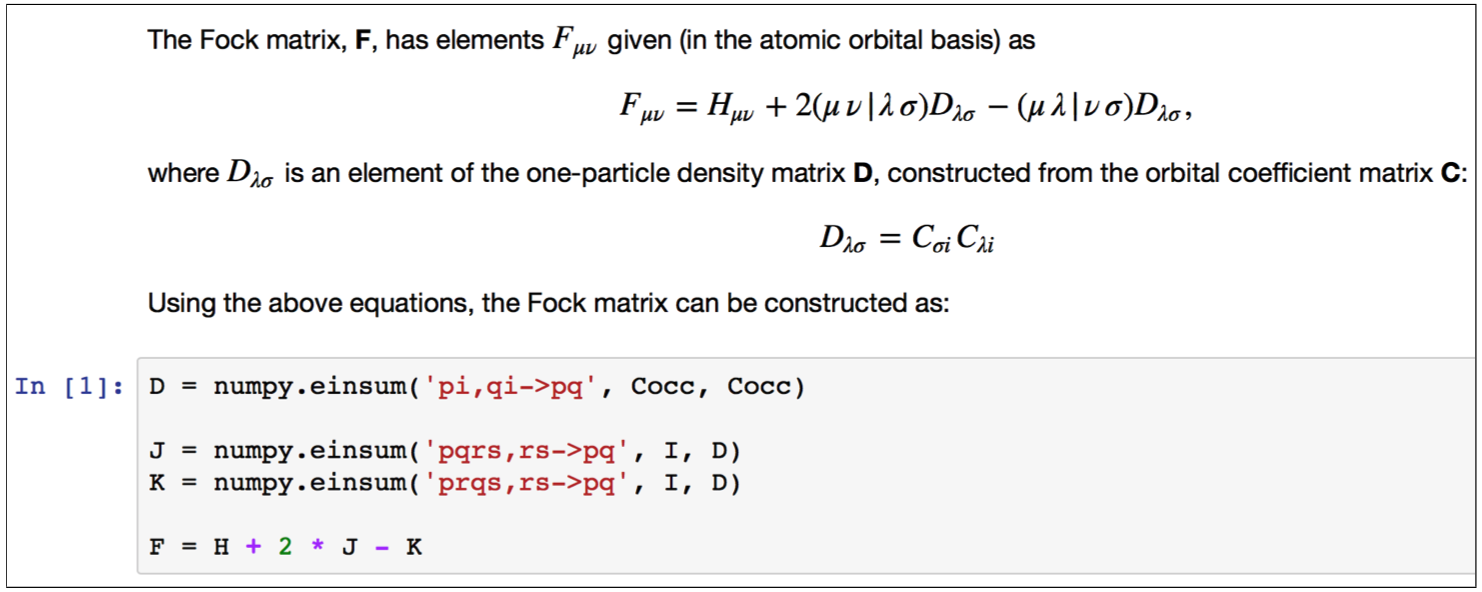
\includegraphics[scale=0.25]{paper_05/fig2.png}
  \caption{Extract from a Jupyter notebook demonstrating the construction of a SCF Fock matrix where {\tt I} is the 4-index electron repulsion integral array and {\tt Cocc} is the occupied orbital matrix.}
  \label{fig:ipython}
\end{figure}

These documents may be unique within quantum chemistry in that they focus not only on theoretical considerations but also on the details of a method's implementation, such as \emph{why} certain programming choices were made. For example, the comparison between a general matrix inversion and solving a set of linear equations demonstrates instability issues that often plague the former technique. Such illustrations should make the Jupyter implementations useful both to new users in quantum chemistry and to experienced users interested in exploring new subfields.

% Whether a theorist wanting to learn or brush up on new quantum chemical methods or an instructor assembling a QC methods workshop, \pfn is a valuable resource. In particular, a learner is advised to read the introductory tutorial, \pfn Basics, then go directly to the implementation scripts, referring back to the later tutorials for enrichment, if needed.  An instructor will want to focus on the tutorials, perhaps devising exercises at the end of each for students to develop their syntax and method skills.

% Whether a student or enthusiast wanting to learn or brush up on quantum chemical methods, a prospective developer seeking good practices for manipulating \pfour's powerful C++ backend, an instructor assembling a QC methods or \pfour users workshop, or a researcher in need of a reference implementation validation, \pfn is a valuable resource. In particular, a learner is advised to read the introductory tutorial, \pfn Basics, then go directly to the implementation scripts, referring back to the later tutorials for enrichment, if needed. A developer should start with a familiar method, then examine all the variations and implementations to see how it's expressed for \pfour. An instructor (unless for an advanced workshop) will want to focus on the tutorials, perhaps devising exercises at the end of each for students to develop their syntax and method skills. A researcher whose target method is lodged with \pfn will naturally focus on adding variations to that script, validating his own code against them, and hopefully contributing his improvements back to \pfn.

Current tutorial-style Jupyter reference implementations include

\begin{enumerate}
\item Introductions to the \pfn methodology
\item Introduction to Hartree--Fock, DIIS, and density fitting
\item Density Functional Theory: grids, LDA kernels, VV10 dispersion, and asymptotic corrections
\item M\o ller--Plesset: canonical and density-fitted reference implementations of MP2
\item Molecular Properties: Integrals, CPHF, CIS
\item Symmetry-Adapted Perturbation Theory: Canonical and atomic orbital algorithms
\item Orbital-Optimized Methods: OMP2
\item Coupled-Cluster Approximations: CEPA0, CCD
\item  Geometry Optimization Techniques: Internal Coordinates, Hessian guesses, and advanced Newton-Raphson methods
\end{enumerate}
Molecular-dynamics tutorials include
\begin{enumerate}
\item Periodic Lennard-Jones simulation with Verlet integrators
\item Periodic Ewald Electostatic summation
\end{enumerate}

\section{Conclusions}

We believe that the benefits of the \pfn framework to the computational chemistry community are threefold.  Beginning researchers can use the \pfn reference implementations for \emph{education}. Reference implementations convey not just the underlying mathematical formulas of a given theory, but how to implement these formulas in a manner that avoids common pitfalls such as ill-conditioned numerical equations. \pfn is likely the most interactive educational resource available in this field: thanks to the Jupyter Notebook format, the learners can explore the implementation step by step and easily try out various modifications and additional approximations.

More advanced researchers who need to reimplement and/or modify a given computational chemistry approach can use the \pfn reference implementations for \emph{validation}, taking advantage of the code that, thanks to the extensive use of the \numpy \texttt{einsum} functionality, provides a nearly one-to-one correspondence between the terms in a formula and the lines of Python code. As a result, it is trivial to switch off, for debugging purposes, any subset of terms as well as generate an arbitrary intermediate without even recompiling any code.  This feature should be contrasted with the situation when one tries to validate their code against a C++/Fortran implementation from an established electronic-structure package. Once the relevant fragment of code that does the actual computation is found (which is not always trivial), various terms are typically combined in nontrivial ways to improve computational performance. As a result, getting out a specific intermediate for checking the implementation in progress often requires substantive changes to the reference code, not to mention its recompilation.  In addition, we include the programmed formulas together with their implementation in the Jupyter Notebook to alleviate difficulties associated with incompatible notation or even errors in the originally published expressions.

Finally, for researchers who want to develop new functionality, \pfn is a highly valuable platform for \emph{initial implementation} that is efficient enough for meaningful testing, quick to generate, easy to debug, and has few opportunities for programming errors. All underlying quantum-chemistry building blocks such as integrals, orbitals, density matrices, and CI vectors are efficiently computed by \pfour and readily imported in the \numpy format. In particular, a \pfn implementation of any one-electron theory such as HF or DFT is already close to optimal as the most expensive operations are all written in terms of generalized Coulomb and exchange matrices which are supplied by \pfour.  Some of us, together with their collaborators, have already taken advantage of the \pfn capabilities to rapidly generate pilot implementations of brand new electronic-structure approaches.

\section{Associated Content}
Documents reproducing all currently available reference implementations and interactive tutorials are available free of charge via the Internet at \url{https://zenodo.org/record/1134320}. For all future materials, please see \url{https://github.com/psi4/psi4numpy}.

\section{Acknowledgements}
This work was supported in part by the U.S.~National Science Foundation through grants ACI-1449723 and CHE-1566192 for D.G.A.S, L.A.B., D.A.S, and C.D.S; CHE-1661604 for B.Z., A.S.A, J.M.T., and H.F.S; CHE-1554354 for D.R.N and A.E.D. B. Z. contributions to this work were also supported by a Software Fellowship from the Molecular Sciences Software Institute, which is funded by the U.S. National Science Foundation (ACI-1547580).  M.H.L. acknowledges financial support by the Studienstiftung des Deutschen Volkes. K.P.  is supported by the U.S. National Science Foundation CAREER award CHE-1351978.

%
\bibliographystyle{achemso}
\safebibliography{paper_04/paper,paper_05/psi4numpy}
%
\end{document}
